\documentclass[11pt,a4paper]{article}

\usepackage[utf8]{inputenc}
\usepackage[T1]{fontenc}
\usepackage{amsmath,amssymb,amsfonts,mathtools}
\usepackage{amsthm}
\usepackage{booktabs}
\usepackage{array}
\usepackage{longtable}
\usepackage{float}
\usepackage{enumitem}
\usepackage{geometry}
\usepackage{hyperref}
\usepackage{xcolor}
\usepackage{tikz}
\usetikzlibrary{positioning,arrows.meta,shapes.geometric,fit,calc}
\geometry{margin=1in}
\hypersetup{colorlinks=true, linkcolor=blue, citecolor=blue, urlcolor=blue}
\setlength{\parindent}{0pt}
\setlength{\parskip}{0.45em}
\emergencystretch=3em
\setcounter{tocdepth}{2}

\newtheorem{theorem}{Theorem}[section]
\newtheorem{lemma}[theorem]{Lemma}
\newtheorem{proposition}[theorem]{Proposition}
\newtheorem{corollary}[theorem]{Corollary}
\newtheorem{definition}[theorem]{Definition}
\newtheorem{assumption}[theorem]{Assumption}
\newtheorem{remark}[theorem]{Remark}
\newtheorem{limitation}[theorem]{Limitation}
\newtheorem{interpretation}[theorem]{Interpretation}
\newtheorem{conclusion}[theorem]{Conclusion}

\newcommand{\D}{\mathcal D}
\newcommand{\Hcal}{\mathcal H}
\newcommand{\Ccal}{\mathcal C}
\newcommand{\Lcal}{\mathcal L}
\newcommand{\Pcal}{\mathcal P}
\newcommand{\Acal}{\mathcal A}
\newcommand{\Kcal}{\mathcal K}
\newcommand{\Vcal}{\mathcal V}
\newcommand{\OmegaCal}{\Omega}
\newcommand{\Rcal}{\mathcal R}
\newcommand{\Ecal}{\mathcal E}
\newcommand{\Fcal}{\mathcal F}
\newcommand{\Xcal}{\mathcal X}
\newcommand{\Ycal}{\mathcal Y}
\newcommand{\Gcal}{\mathcal G}
\newcommand{\Qcal}{\mathcal Q}
\newcommand{\Mcal}{\mathcal M}
\newcommand{\Tcal}{\mathcal T}
\newcommand{\Bcal}{\mathcal B}
\newcommand{\Scal}{\mathcal S}
\newcommand{\Dcal}{\mathcal D}
\newcommand{\Ucal}{\mathcal U}
\newcommand{\calib}{\mathrm{cal}}
\newcommand{\hold}{\mathrm{hold}}
\newcommand{\stress}{\mathrm{stress}}
\newcommand{\adv}{\mathrm{adv}}
\newcommand{\shift}{\mathrm{shift}}
\newcommand{\NOCert}{\operatorname{NOCert}}
\newcommand{\Tr}{\operatorname{Tr}}
\newcommand{\supp}{\operatorname{supp}}
\newcommand{\argmax}{\operatorname*{arg\,max}}
\newcommand{\argmin}{\operatorname*{arg\,min}}
\newcommand{\id}{\mathrm{id}}
\newcommand{\eps}{\varepsilon}
\newcommand{\RCP}{\mathrm{RCP}}
\newcommand{\RCLM}{\mathrm{RCLM}}
\newcommand{\RSI}{\mathrm{RSI}}
\newcommand{\AC}{\mathrm{AC}}
\newcommand{\DG}{\mathrm{DG}}
\newcommand{\sem}{\mathrm{sem}}
\newcommand{\sys}{\mathrm{sys}}
\newcommand{\ctx}{\mathrm{ctx}}
\newcommand{\arch}{\mathrm{arch}}
\newcommand{\rec}{\mathrm{rec}}
\newcommand{\safe}{\mathrm{safe}}
\newcommand{\state}{\mathrm{state}}
\newcommand{\true}{\mathrm{true}}
\newcommand{\aud}{\mathrm{aud}}
\newcommand{\raw}{\mathrm{raw}}
\newcommand{\mix}{\mathrm{mix}}
\newcommand{\loss}{\mathrm{loss}}
\newcommand{\amb}{\mathrm{amb}}
\newcommand{\IB}{\mathrm{IB}}
\newcommand{\rel}{\mathrm{rel}}
\newcommand{\op}{\mathrm{op}}
\providecommand{\Cap}{\operatorname{Cap}}
\newcommand{\SafeCap}{\operatorname{SafeCap}}
\newcommand{\Risk}{\operatorname{Risk}}
\newcommand{\Val}{\operatorname{Val}}
\newcommand{\Cert}{\operatorname{Cert}}
\newcommand{\Sound}{\operatorname{Sound}}
\newcommand{\Power}{\operatorname{Power}}
\newcommand{\Cost}{\operatorname{Cost}}
\newcommand{\Budget}{\operatorname{Budget}}
\newcommand{\dist}{\operatorname{dist}}
\newcommand{\margin}{\operatorname{margin}}
\newcommand{\softmax}{\operatorname{softmax}}
\newcommand{\diag}{\operatorname{diag}}
\newcommand{\vecop}{\operatorname{vec}}
\newcommand{\ProjD}{\Pi_{\D}}
\newcommand{\ProjK}{\Pi_{\Kcal}}
\newcommand{\collapse}{\mathrm{collapse}}
\newcommand{\irreversible}{\mathrm{irreversible}}
\newcommand{\misgrounded}{\mathrm{misgrounded}}
\newcommand{\misalignment}{\mathrm{misalignment}}
\newcommand{\selferror}{\mathrm{self\mbox{-}error}}
\newcommand{\ambcollapse}{\mathrm{amb\mbox{-}collapse}}
\newcommand{\halt}{\mathrm{halt}}
\newcommand{\LM}{\mathrm{LM}}
\newcommand{\reg}{\mathrm{reg}}
\newcommand{\mem}{\mathrm{mem}}
\newcommand{\ver}{\mathrm{ver}}
\newcommand{\phys}{\mathrm{phys}}
\newcommand{\asy}{\mathrm{asy}}
\newcommand{\verify}{\mathrm{verify}}
\newcommand{\data}{\mathrm{data}}
\newcommand{\test}{\mathrm{test}}
\newcommand{\val}{\mathrm{val}}
\newcommand{\search}{\mathrm{search}}
\newcommand{\cert}{\mathrm{cert}}
\newcommand{\cost}{\mathrm{cost}}
\newcommand{\apply}{\mathrm{apply}}
\newcommand{\tools}{\mathrm{tools}}
\newcommand{\update}{\mathrm{update}}
\newcommand{\upd}{\mathrm{upd}}
\newcommand{\local}{\mathrm{local}}
\newcommand{\soft}{\mathrm{soft}}
\newcommand{\hard}{\mathrm{hard}}
\newcommand{\qtype}{\mathrm{q}}
\newcommand{\cltype}{\mathrm{cl}}
\newcommand{\reptype}{\mathrm{repr}}
\newcommand{\emb}{\mathrm{emb}}
\newcommand{\coup}{\mathrm{coup}}
\newcommand{\trust}{\mathrm{trust}}
\newcommand{\trustadv}{\mathrm{trustadv}}
\newcommand{\anchor}{\mathrm{anchor}}
\newcommand{\support}{\mathrm{support}}
\newcommand{\graph}{\mathrm{graph}}
\newcommand{\sole}{\mathrm{sole}}
\newcommand{\edge}{\mathrm{edge}}
\newcommand{\sound}{\mathrm{sound}}
\newcommand{\power}{\mathrm{power}}
\newcommand{\scale}{\mathrm{scale}}
\newcommand{\noop}{\mathrm{noop}}
\newcommand{\infl}{\mathrm{infl}}
\newcommand{\gate}{\mathrm{gate}}
\newcommand{\tot}{\mathrm{tot}}
\newcommand{\avail}{\mathrm{avail}}
\newcommand{\res}{\mathrm{res}}
\newcommand{\rollback}{\mathrm{rollback}}
\newcommand{\eval}{\mathrm{eval}}
\newcommand{\suite}{\mathrm{suite}}
\newcommand{\repro}{\mathrm{repro}}
\newcommand{\metric}{\mathrm{metric}}
\newcommand{\stat}{\mathrm{stat}}
\newcommand{\model}{\mathrm{model}}
\newcommand{\Rec}{\operatorname{Rec}}
\newcommand{\cov}{\mathrm{cov}}
\newcommand{\trk}{\mathrm{trk}}
\newcommand{\untrk}{\mathrm{untrk}}
\newcommand{\ood}{\mathrm{ood}}
\newcommand{\est}{\mathrm{est}}
\newcommand{\prot}{\mathrm{prot}}
\newcommand{\engine}{\mathrm{engine}}
\newcommand{\NLRSI}{\mathrm{NL\mbox{-}RSI}}
\newcommand{\NL}{\mathrm{NL}}
\newcommand{\IsoExt}{\mathrm{IsoExt}}
\newcommand{\AppendMem}{\mathrm{AppendMem}}
\newcommand{\RevAdapter}{\mathrm{RevAdapter}}
\newcommand{\VerifierExt}{\mathrm{VerifierExt}}
\newcommand{\ToolExt}{\mathrm{ToolExt}}
\newcommand{\NLalg}{\mathrm{NLalg}}
\newcommand{\call}{\mathrm{call}}
\newcommand{\TC}{\mathrm{TC}}
\newcommand{\RSIPot}{\operatorname{RSIPot}}
\newcommand{\ProjReal}{\operatorname{ProjReal}}
\newcommand{\Trans}{\operatorname{Trans}}
\newcommand{\CE}{\mathrm{CE}}
\newcommand{\Eng}{\mathrm{Eng}}
\newcommand{\Lift}{\operatorname{Lift}}
\newcommand{\advtrust}{\mathrm{advtrust}}

\newcommand{\CorrFail}{\operatorname{CorrFail}}
\newcommand{\AuditLeak}{\operatorname{AuditLeak}}
\newcommand{\CommonMode}{\operatorname{CommonMode}}
\newcommand{\CollusionRisk}{\operatorname{CollusionRisk}}
\newcommand{\CovGap}{\operatorname{CovGap}}
\newcommand{\CxCost}{\operatorname{CxCost}}
\newcommand{\SelfTrans}{\operatorname{SelfTrans}}


\title{RSI--RCLM Final v1: A Domain-Relative Robust Reflective Successor Theorem for Certified RCLM Seed-Library Classes with Batch-13R/13R-A/13R-B Reference Entry, Controlled Executable Artifacts, Mechanization Certificates, and M3-Min Learned-Agent Entry Boundary}
\author{Nicolas Calder\\[0.25em]\small\texttt{n926mp@gmail.com}}
\date{June 29, 2026}

\begin{document}
\maketitle

\begin{abstract}
This manuscript is the final v1 architecture realization of the Recursive Coherence Language Model with Trainable Hamiltonians (RCLM--TH) under the updated Batch-13R reference-entry, proof-carrying successor-construction, concrete finite reference-witness, controlled executable reference-system, external-mechanization-boundary, M3-Min learned-entry-boundary, and artifact-ready Recursive Coherence Preservation (RCP) math/physics framework.  The reference paper distinguishes the already-proved \emph{Conditional Non-Lossy Self-Update Preservation Theorem} from the still-conditional \emph{Direct Non-Lossy RSI Engine Theorem} target, and it adds the conservative-extension algebra \(\mathfrak G^{\mathrm{NL}}\) as a certified non-lossy update class, the tangent-cone local progress theorem as a conditional local construction rule, and an engine-viability nonemptiness theorem for conservative-extension systems.  This architecture paper synchronizes with that framing.  Its central theorem is an architecture-level conditional preservation and instantiation theorem: if the RCLM system supplies the required typed density states, representation-to-density embeddings, semantic-coupling maps, non-oracular certificates, trust-graph support, adaptive-audit trust support, coverage/calibration/estimator subprotocols, resource ledgers, and viability assumptions, then accepted RCLM self-updates inherit the recoverable non-loss, Lyapunov stability, semantic-validity, verifier, resource, capability, and asymptotic preservation guarantees of the RCP theorem stack.

The central architectural correction remains unchanged: the internal recursive coherence operator \(\Rcal_{\theta}\) is not the same object as the recursive self-improvement channel \(\Phi_t\).  The operator \(\Rcal_{\theta}\) is the Level 2 inference dynamics acting on context-level language states through trainable Hamiltonian layers.  The channel \(\Phi_t\) is the Level 3 self-modification map acting on the system-level state that encodes parameters, architecture, memory, verifier, barriers, semantic maps, resource state, capability model, and self-model.  The architecture becomes a candidate RSI system only when proposed self-updates are admitted by the fully augmented RCP gate \(\Acal_{\RCP}^{\RCLM\text{-}\DG}(t,\rho_t^{\sys})\).

The thesis is now phrased as \emph{recoverable monotone self-improvement}.  Safety is treated as a corollary of recoverable non-loss applied to a declared subfamily of protected predicates, not as a separate magic property.  This paper therefore defines an RCLM protected-predicate hierarchy, records the architecture-level target engine object
\[
\mathfrak E_t^{\RCLM}:\rho_t^{\sys}\mapsto(\nu_t,\Phi_{\nu_t},\mathcal R_{\Phi_{\nu_t}}^{\rec},\mathsf{Cert}_t,\rho_{t+1}^{\sys}),
\]
and, after Batch 9, proves a domain-restricted \emph{Direct Non-Lossy RSI Engine Theorem} for states inside a declared direct-engine domain with strict beneficial conservative-extension witnesses, generator coverage, certificate soundness, and successor-viability margins.  The present manuscript does not prove that arbitrary RCLM systems lie in that domain or that every learned lift produces useful primitive words.  It instantiates the Batch-3 algebraic non-loss layer by defining RCLM non-lossy primitive generators, transported pair sets, word-level composition, additive loss/recovery budgets, and an algebraic non-loss subgate.  It instantiates the Batch-4 tangent-cone layer by defining local RCLM residuals \(q_{t,j}^{\RCLM}(\nu)\le0\), the admissible tangent cone \(T_{\Acal_t^{\RCLM}}\), the RSI potential functional \(\RSIPot_t\), and the projected tangent-cone gradient \(P_{T_{\Acal_t^{\RCLM}}}\nabla_\nu\RSIPot_t\).  It instantiates the Batch-5 engine-viability layer by defining RCLM engine-base sets, conservative-extension engine moves, finite-horizon and infinite-horizon RCLM engine viability kernels, certified extension plans, and the theorem that membership in the declared kernel yields a non-lossy conservative-extension update whose successor remains in the next kernel.  This Batch-6 version adds the missing RCLM lift layer
\[
\mathsf{Lift}_t:(\rho_t^{\ctx,*},M_t,W_t,\mathcal H_t^{\cert})\to\Omega_t^{\NL,\RCLM},
\]
which maps halted Level 2 recursive-coherence inference outputs, self-model state, verifier state, and certificate history into certified non-lossy primitive-word candidates.  It also adds a minimal finite-dimensional reference engine showing, in a completely explicit conservative-extension model, that protected distinctions are preserved exactly, a recovery map is explicit, predecessor abilities are retained by callable fallback, and a certified new ability yields strict ability-set expansion.  The result is still conditional: it proves lift-soundness and a finite reference construction under stated certificates, not that arbitrary RCLM systems automatically generate useful lifted primitive words or that empirical frontier-scale certification is solved.

This Batch-9 synchronization adds the RCLM direct-engine constructor \(\mathfrak E_t^{\RCLM}\) as a generator-certifier-selector-realizer pipeline.  On the declared direct-engine domain \(\Dcal_t^{\RCLM\text{-}\engine}\), the constructor generates a finite non-lossy primitive-word set, certifies candidates through the full Batch-1--8 gate stack, selects a passing beneficial conservative-extension word, realizes the accepted update, and returns a recovery map, certificate packet, and successor state.  The corresponding theorem proves construction, not merely verification, but only under explicit strict-witness, generator-coverage, certificate-soundness, resource, projection-realization, and successor-kernel assumptions.

This Batch-7 version adds publication-rigor scaffolding: a theorem-type table separating algebraic, telescoping, certificate-composition, assumption-dependent existence, reference-engine, and implementation-status results; an implementation-status table separating specified, assumed, reference-implemented, audited, empirically validated, and not-yet-validated architecture objects; and an explicit claim-discipline rule that prevents certificate plumbing, reference-engine demonstrations, and protocol definitions from being misread as empirical validation or unconditional RSI solution theorems.

This Batch-8 version synchronizes the architecture with the updated RCP cross-time/state-update/projection cleanup. It adds explicit RCLM transport maps for question, evidence, self-model, future-behavior, and update-description variables; separates state-only safe sets from update-dependent admissibility relations; splits state Lyapunov monitoring from candidate-indexed update Lyapunov residuals; and adds a projection-realization certificate so that a mathematically projected safe state is not treated as an accepted self-update unless a typed RCLM update realizes it within declared distortion.


This Batch-10 version adds the remaining architecture-publication cleanup requested by the pro-model evaluation: adaptive-audit trust modeling, an explicit architecture complexity/scalability ledger, and a terminology cleanup separating generic typed self-update transitions from literal quantum or stochastic channels.  The strengthened adaptive trust layer defines correlated verifier failure, audit leakage, common-mode support risk, and collusion risk.  The new gate \(\Acal_{\trust}^{\adv}\) requires verifier-changing candidates to satisfy the previous no-self-sole-certification rule and to remain below audited bounds for common-mode, collusion, leakage, and correlated-failure risk.  The complexity ledger records dominant costs for Hamiltonian exponentials, eigendecompositions, spectral powering, residual estimators, candidate search, and direct-engine certification.  It is an accounting and publication-readiness device, not a proof of frontier-scale tractability.  Finally, throughout this paper \(\Phi_\nu\) is interpreted generically as a typed self-update transition; it is called a channel only when a CPTP, stochastic, or equivalent channel certificate is supplied.


This Batch-11 version synchronizes the architecture with the new RCP domain-nonemptiness and witness-library closure theorem.  It adds an RCLM seed engine domain \(\Kcal_t^{\RCLM\text{-}\mathrm{seed},N}\), certified conservative-extension module libraries \(\Lcal_t^{\RCLM\text{-}\CE}\), library descriptors in the self-model, bounded non-lossy primitive-word grammars, RCLM library-lift coverage certificates, direct-engine domain entry from seed packages, explicit seed-equivalence/persistence-transfer certificates \(\mathsf{SeedEq}_t^{\RCLM}\), successor seed-domain invariance, and finite direct-engine trajectories from seed domains.  This discharges the Batch-9 direct-engine-domain assumption only for declared bounded seed/library classes; it still does not prove that arbitrary trained RCLM systems naturally enter those classes.

This Batch-12 / Batch-12A version synchronizes the architecture with the RCP-II Phase-1 successor-verification layer.  It adds an RCLM successor-verification seed domain \(\Kcal_t^{\RCLM\text{-}\mathrm{SV},N}\subseteq\Kcal_t^{\RCLM\text{-}\mathrm{seed},N}\), successor-verification schemas \(\mathsf{VerSch}_t^{\RCLM\text{-}\mathrm{SV}}\), uncertainty envelopes \(\Pcal_t^{\RCLM\text{-}\mathrm{SV}}\), goal-identity transport certificates, successor-verification progress functionals, certificate packets \(\mathsf{SVPkg}_t^{\RCLM}(\rho,\nu)\), explicit Batch-12A residual vectors \(Q_t^{\RCLM\text{-}\mathrm{SV},A}\), verifier-schema transport dynamics, uncertainty-envelope transport, goal-identity composition, anti-circular reflective-trust residuals, an algorithmic successor-verification gate, and a domain-invariance theorem showing that a Batch-11 seed-domain engine step can preserve the stronger successor-verification seed domain when the corresponding explicit certificates are valid.  This is a restricted certificate-reflective theorem, not a proof of universal Vingean reflection, full L\"obian self-trust, arbitrary world-model correctness, or scalable proof search.


This Batch-12B version adds the corresponding architecture-side packet-construction and closure layer.  It defines the RCLM successor-verification packet builder \(\mathsf{SVBuilder}_t^{\RCLM}\), the RCLM packet-construction domain \(\Dcal_t^{\RCLM\text{-}\mathrm{SV\mbox{-}construct}}\), RCLM successor-verification witness libraries \(\Lcal_t^{\RCLM\text{-}\mathrm{SV\mbox{-}Wit}}\), finite and infinite RCLM successor-verification seed-library domains, reality-containment/misspecification certificates \(\mathsf{RealCont}_t^{\RCLM}\), restricted tractability certificates \(\mathsf{SVTract}_t^{\RCLM}\), and a domain-relative RCLM robust reflective successor theorem.  Batch 12B therefore closes the Batch-12A packet-existence gap only for declared RCLM seed-library classes: it proves packet construction, seed-domain entry, and infinite generated-path closure when the stated libraries, grammars, builders, reality-containment certificates, and cost certificates are valid.  It still does not prove arbitrary trained-system entry, universal successor trust, or full L\"obian/Vingean reflection.

This finalization and instantiation-readiness version surfaces the result under its strongest honest title: a domain-relative, certificate-relative robust reflective successor theorem for certified RCLM seed-library classes.  It adds a paper-ready theorem surfacing layer, a minimal finite RCLM successor-verification reference-instance target, an implementation-readiness boundary, a main-goal fit and qualification table, and an implementation roadmap.  These additions do not create a new abstract theorem batch; they mark the current architecture theorem as a substantial conditional endpoint and identify the next frontier as reference instantiation, implementation, and empirical validation.

This Batch-13R reference-entry version now adds that next frontier inside the architecture paper without creating a new abstract successor theorem.  It defines finite RCLM reference classes, proof-carrying successor packets \(\mathsf{PCS}_t^{\RCLM}\), a finite checker \(\mathsf{Check}_{\RCP}^{\RCLM}\), a reference builder \(\mathsf{BuildRefSV}_{0:N}^{\RCLM}\), and the theorem
\[
\mathsf{BuildRefSV}_{0:N}^{\RCLM}(\mathcal M,\mathcal D,\mathcal L,\mathcal C)
\Downarrow
\mathsf{RefSV}_{0:N}^{\RCLM}
\Longrightarrow
\rho_0^{\sys}\in
\Kcal_0^{\RCLM\text{-}\mathrm{SV\mbox{-}seedlib},N}.
\]
It also adds a canonical finite RCLM appended-module reference witness, a proof-carrying finite certified trajectory, restricted tractability for the declared finite representation class, singleton simulated-environment reality containment, and a replayable artifact theorem.  This upgrades the finite reference target from a merely specified object to a finite-witnessed, proof-carrying restricted Scenario-3 reference construction, while still not claiming arbitrary trained-system entry or frontier-scale validation.

This Batch-13R-A synchronization adds the final architecture-side rigor patch corresponding to the concrete finite RCP reference witness. It makes the canonical explicit successor-verification residual vector part of the RCLM construction, proves that the canonical checker realizes those residuals, adds an artifact parser/replay soundness theorem, and states an explicit refinement map from the canonical RCLM witness to the canonical RCP witness.

This Batch-13R-B milestone version adds the pre-publication architecture-side distinction between an externally mechanized reference artifact and a controlled executable reference system.  It defines the narrow mechanization target \(\mathsf{MechTarget}_{0:N}^{\RCLM,\mathrm{can}}\), the external proof-assistant certificate object \(\mathsf{MechCert}_{0:N}^{\RCLM,\mathrm{can}}\), the controlled executable reference object \(\mathsf{CtrlRef}_{0:N}^{\RCLM}\), and the replay certificate \(\mathsf{CtrlReplayCert}_{0:N}^{\RCLM}\).  The paper explicitly distinguishes a Python, shell, or notebook replay artifact from an external Lean/Coq/Isabelle/Agda-style proof-kernel certificate.  In the current companion artifact package, a shared Lean 4 project supplies a narrow external certificate for the canonical finite RCP/RCLM witness, the finite checker core, and the RCLM-to-RCP refinement module: \(\texttt{RCP.lean}\), \(\texttt{RCLM.lean}\), the root module \(\texttt{RcpRclmMech.lean}\), and the library build all check successfully.  This licenses the qualified claim that the canonical finite RCP/RCLM witness and refinement core are Lean-checked.  It does not license the claim that the full 219-page math stack, the full 187-page architecture stack, arbitrary learned-system entry, broad capable-agent RSI, or empirical deployment behavior is fully mechanized.

This M3-Min version adds the minimal learned-agent entry boundary corresponding to the controlled learned-system audit protocol in the reference RCP paper.  It defines a controlled learned RCLM class \(\mathsf{LearnedRCLMClass}_{n,k,N}^{\mathrm{ctrl}}\), a learned-entry certificate packet \(\mathsf{LECert}_{0:N}^{\RCLM}\), a learned-entry audit procedure \(\mathsf{LearnedEntryAudit}_{0:N}^{\RCLM}\), a conditional theorem showing that any controlled learned RCLM system returning a full learned-entry certificate enters \(\Kcal_0^{\RCLM\text{-}\mathrm{SV\mbox{-}seedlib},N}\), and a partial-pass / controlled trained-system pilot protocol.  This is not a broad learned-agent theorem: it formalizes the finite certificate boundary a learned system must satisfy before invoking the existing Batch-13R theorem stack.

\end{abstract}

\textbf{Keywords:} recursive coherence language model, recoverable monotone self-improvement, recursive self-improvement, recursive self-modeling, trainable Hamiltonians, Recursive Coherence Preservation, Conditional Non-Lossy Self-Update Preservation Theorem, Direct Non-Lossy RSI Engine Theorem, Lyapunov stability, relative entropy, barrier certificates, semantic validity, verifier bootstrapping, verifier trust graphs, budgeted certified search, persistent improvement, resource-scaling closure, no-op monitoring, certificate inflation, reproducible evaluation, capability preservation, non-lossy RSI, conservative extension algebra, tangent-cone local progress, engine viability, RCLM lift, finite-dimensional reference engine, RSI potential, cross-time transport, state/update separation, projection-realization certificate, direct engine constructor, constructive beneficial extension, adaptive audit, common-mode verifier risk, architecture complexity ledger, typed self-update transition, seed-domain entry, witness-library closure, bounded primitive-word grammar, RCLM lift coverage, seed-equivalence certificate, successor-verification seed domain, RCLM successor-verification schema, uncertainty envelope, goal-identity transport, explicit successor-verification residuals, algorithmic successor-verification gate, successor-verification packet builder, SV witness library, SV seed-library nonemptiness, infinite generated SV domain, reality-containment certificate, restricted SV tractability certificate, domain-relative robust reflective successor theorem, reference-instantiation readiness, implementation boundary, main-goal fit table, finite RCLM SV reference instance, Batch-13R, proof-carrying successor packet, RCLM reference builder, RCLM reference checker, canonical finite RCLM reference witness, executable reference artifact, finite certified successor trajectory, Batch-13R-A, canonical explicit SV residual vector, canonical checker realization, artifact parser, RCLM-to-RCP reference refinement, Batch-13R-B, external mechanization certificate, controlled executable reference system, controlled replay certificate, proof-assistant mechanization boundary, Lean 4 certificate, mechanization status manifest, M3-Min, learned-agent entry boundary, controlled learned-system audit, learned RCLM entry certificate, controlled trained-system pilot, partial-pass reporting protocol.

\noindent\textbf{Companion manuscript and artifact status.}\quad
This manuscript is Paper II of a two-paper package.  Paper I gives the architecture-general RCP/RCP-II theorem stack; this paper gives the RCLM architecture realization, reference-entry construction, controlled artifact layer, and learned-entry boundary.  The shared artifact repository contains the Lean 4 proof project, controlled RCP/RCLM reference artifacts, replay checkers, run logs, theorem map, and mechanization manifest.  The Lean 4 certificate is supplied for the canonical finite RCP/RCLM witness, the finite checker core, and the RCLM-to-RCP refinement module.  The certificate does not mechanize the full 219-page math stack, the full 187-page architecture stack, arbitrary trained-system entry, broad capable-agent RSI, or empirical deployment claims.

\tableofcontents
\newpage

\section{Purpose and Relationship to the Math/Physics Paper}

The purpose of this document is to realize the full Batch-13R / Batch-13R-A / Batch-13R-B reference-entry, proof-carrying successor-construction, concrete finite reference-witness, controlled executable reference-system, external-mechanization-boundary, and M3-Min learned-entry-boundary RCP math/physics paper inside a concrete RCLM--TH-derived architecture. The prior architecture manuscript used only the compact RCP core. This final v1 architecture uses the operationally closed, recoverable-monotone, conservative-extension, tangent-cone, engine-viability, lift/reference-engine, theorem-type, cross-time/projection-realization, direct-engine-construction, seed-domain/witness-library, successor-verification residual, and Batch-12B packet-construction/infinite-closure plus Batch-13R reference-entry/proof-carrying theorem stack and the M3-Min learned-entry audit boundary.

The construction is:
\[
\begin{aligned}
&\text{RCLM--TH substrate}
+\text{recoverable-monotone operational RCP preservation stack}\\
&\hspace{2.5cm}\longrightarrow\text{RCP-gated RSI--RCLM final v1}.
\end{aligned}
\]

The first paper is architecture-general. It now distinguishes the conditional preservation theorem that is already proved from the direct engine theorem that remains to be built. It defines what a non-lossy recursive self-improvement process must preserve and how safety appears as a corollary when safety predicates are included in the protected predicate family. This second paper is architecture-specific. It asks how an RCLM with trainable Hamiltonian recursive coherence dynamics can instantiate those preservation constraints without pretending that the direct engine theorem has already been constructed.

\begin{remark}[Architectural role]
This document should not be read as a replacement for the RCP theorem paper. It is the applied realization paper. The theorems here are mostly instantiation theorems: they show that, once the architecture provides objects satisfying the RCP hypotheses, the corresponding RCLM updates inherit the RCP guarantees.
\end{remark}


\subsection{Non-repetitive completion criterion for the architecture paper}

Because the updated Batch-13R-B RCP math/physics paper is now the reference theorem stack, this architecture paper does not need to re-prove every RCP lemma, drift theorem, barrier theorem, recoverability result, closure module, seed-domain entry theorem, successor-verification residual theorem, packet-construction theorem, infinite-horizon reflective-closure theorem, proof-carrying reference-entry theorem, or concrete finite reference-witness theorem, external-mechanization-certificate statement, or controlled executable reference-system theorem, or the M3-Min learned-entry boundary theorem. Repeating those proofs would make the document longer without making the RCLM realization more complete. The architecture paper is complete relative to the math/physics reference when it supplies the missing architecture-specific objects required to instantiate those theorems inside the RCLM setting.

Under that standard, the non-repetitive obligations are the following five items:
\begin{enumerate}[label=(\arabic*),leftmargin=1.5em]
    \item \textbf{Architecture-specific state construction and type realization.} The paper must specify how tokens, hidden states, objective projections, subjective projections, ambiguity/definitiveness heads, self-model heads, memory, verifier state, and resource state become the system state
    \[
    \rho_t^{\sys}\in\D(\Hcal_{\RCP}\otimes\Hcal_{\arch}),
    \]
    and must state whether the resulting object is physical-quantum, classical-probabilistic, or representational. Density-matrix notation alone is not allowed to license physical quantum conclusions or semantic conclusions without the corresponding type and coupling certificates.
    \item \textbf{Level 2 recursive inference dynamics.} The paper must specify the internal RCLM recursive coherence map
    \[
    \Rcal_{\theta_t}:\rho_{t,k}^{\ctx}\mapsto\rho_{t,k+1}^{\ctx},
    \]
    including the trainable Hamiltonian evolution, spectral projection, normalization, mixing, monitoring, and halting assumptions.
    \item \textbf{Level 3 self-update dynamics.} The paper must specify the separate self-improvement channel
    \[
    \Phi_{\nu_t}:\rho_t^{\sys}\mapsto\rho_{t+1}^{\sys},
    \]
    including which components may be modified: parameters, projections, Hamiltonians, memory, barriers, verifier, semantic maps, resource model, candidate-update generator, or architecture.
    \item \textbf{Architecture-level RCP gate implementation.} The paper must define how the RCLM candidate update is checked against the full post-D--G gate
    \[
    \Acal_{\RCP}^{\RCLM\text{-}\DG}(t,\rho_t^{\sys}),
    \]
    by specifying typed estimators, audited certificate packets, calibration datasets, stress-test assumptions, one-sided margins, verifier trust graphs, no-self-sole-certification, budgeted certified search, resource-scaling closure, no-op rate monitoring, certificate-inflation penalties, pair-set coverage-gap residuals, coherence--capability calibration checks, residual-specific estimator subprotocols, the RCLM conservative-extension algebra and algebraic non-loss subgate, no-op fallback, rejection, projection, rollback conditions, and a reproducible numerical evaluation protocol for testing the gate without treating protocol definitions as empirical results.
    \item \textbf{Architecture-specific inheritance theorem.} The paper must prove the conditional statement that, if the RCLM objects satisfy the hypotheses of the reference RCP paper, including typed density realization and semantic coupling consistency, then accepted RCLM updates inherit the RCP conclusions. This is not a re-proof of the reference theorem stack; it is the bridge showing that the architecture supplies the theorem inputs.
\end{enumerate}

These five obligations are exactly the parts that would be missing if one merely cited the updated Batch-13R RCP math/physics paper without giving an applied realization. Conversely, the full relative-entropy telescoping proof, Lyapunov drift proof, abstract barrier-certificate proof, abstract closure modules, abstract operational-closure theorem, abstract Batch-11 seed-domain theorem, abstract Batch-12A successor-verification residual theorem, and abstract Batch-12B packet-construction/infinite-closure theorem and Batch-13R reference-entry/proof-carrying witness theorem plus the Batch-13R-B mechanization-boundary, controlled-executable reference theorem, and M3-Min learned-entry boundary theorem belong primarily to the reference RCP paper and are only summarized here when needed for notation.


\subsection{Completion audit of the previous final-v1 architecture draft}

The previous scope-adjusted final-v1 draft correctly identified the five non-repetitive obligations and the seven architecture-specific checklist items, but several of them were still stated at checklist level.  The present version expands them into definitions, assumptions, lemmas, propositions, theorems, algorithms, and toy demonstrations.  In particular, it adds:
\begin{enumerate}[label=(\arabic*),leftmargin=1.5em]
    \item a full architecture-state construction theorem for context and system densities;
    \item a typed density-realization, representation-to-density embedding, and semantic-coupling closure module that prevents category errors between physical density operators, classical probability mixtures, and learned representational states;
    \item a full Level 2 density-preserving dynamics derivation and a conditional finite-recursion stability theorem;
    \item a full Level 3 component-update and accepted-channel construction with no-op, projection, and rollback assumptions;
    \item an estimator-residual implementation of the post-D--G gate and a gate-soundness theorem;
    \item a non-oracular certificate-construction protocol using calibration data, held-out audit data, stress-test families, explicit radii, and one-sided simultaneous soundness events;
    \item a verifier anti-circularity module with trust graphs, no self-sole-certification, and a conditional verifier self-consistency stability theorem;
    \item a persistent-progress and budgeted-search module defining the beneficial safe-improvement set, persistent improvement condition, certified search completeness with budget, and finite-horizon progress theorem;
    \item a resource-scaling and no-op pressure module defining audited cost accounts, amortized scaling closure, no-op rate diagnostics, and bounded certificate-inflation penalties;
    \item a pair-set and adversarial coverage-closure module defining tracked/untracked predicate sets, coverage-gap residuals, adversarial expansion obligations, and audited one-sided coverage bounds;
    \item a conservative-extension algebra module instantiating \(\mathfrak G_{\RCLM}^{\NL}\), RCLM ability-set preservation, structural recovery, primitive word composition, transported pair sets, and additive loss/recovery budgets;
    \item a coherence--capability calibration module defining audited task suites, calibration models, calibration-error gates, and conservative progress-claim transfer;
    \item residual-specific estimator subprotocols for relative-entropy loss, recovery, mutual information, ambiguity collapse, barriers, semantic validity, safe capability, resource cost, verifier integrity, coverage, and calibration residuals;
    \item an architecture-level soft/hard coherence-diversity barrier certificate with no-op feasibility, bounded proposal loss, optimization error, explicit finite-loss bounds, hard forward invariance, and projected safe-state repair;
    \item an explicit architecture-specific inheritance theorem separating what is proved from what is assumed;
    \item concrete inference, self-improvement, and pair-set expansion algorithms;
    \item toy demonstrations showing density preservation, loss-gate acceptance/rejection, and no-op-normalized progress;
    \item a Batch-4 tangent-cone local-progress instantiation, with RCLM residuals, admissible tangent cones, RSI potential, projected tangent-cone gradients, a local progress theorem, and a projected-gradient corollary;
    \item a Batch-5 engine-viability instantiation, with finite-horizon and infinite-horizon RCLM engine kernels, conservative-extension engine move sets, certified extension plans, recursive continuation theorems, and an explicit limitation that kernel nonemptiness is a declared/certified condition rather than an automatic property of arbitrary RCLM states.
    \item a Batch-6 RCLM lift and minimal reference-engine instantiation, with a certified map from halted Level 2 context states to non-lossy primitive-word candidates, a lift-soundness theorem, a lifted engine-continuation theorem, and a finite-dimensional conservative-extension reference construction proving exact protected non-loss, exact recovery, callable predecessor ability preservation, and strict certified ability expansion under explicit assumptions.
    \item a Batch-9 RCLM direct-engine constructor, with generator, certifier, selector, and realizer components, a direct-engine domain, generator-coverage and certificate-soundness assumptions, and a theorem proving that the constructor returns a certified beneficial conservative-extension word whenever its declared domain hypotheses hold.
    \item a Batch-11 RCLM seed-domain and witness-library closure layer, with certified conservative-extension libraries, bounded primitive-word grammars, library-lift coverage, seed-domain entry into the direct-engine domain, seed-equivalence/persistence-transfer certificates, successor seed-domain invariance, and finite seed-domain direct-engine trajectories.
    \item a Batch-12/12A RCLM successor-verification layer, with successor-verification seed domains, verifier-schema transport, uncertainty envelopes, goal-identity transport, explicit SV residual vectors, soundness composition, anti-circular reflective-trust residuals, and a domain-invariance theorem upgrading construction persistence into verification persistence.
    \item a Batch-12B RCLM packet-construction and infinite-closure layer, with \(\mathsf{SVBuilder}_t^{\RCLM}\), RCLM SV witness libraries, finite and infinite SV seed-library domains, generated infinite SV domains, reality-containment certificates, restricted tractability certificates, and a domain-relative RCLM robust reflective successor theorem.
    \item a Batch-13R RCLM reference-entry and proof-carrying layer, with finite RCLM reference classes, \(\mathsf{PCS}_t^{\RCLM}\), \(\mathsf{Check}_{\RCP}^{\RCLM}\), \(\mathsf{BuildRefSV}_{0:N}^{\RCLM}\), a canonical finite appended-module reference witness, a proof-carrying finite certified trajectory, restricted reference tractability, singleton simulated-environment reality containment, and a replayable reference artifact theorem.
    \item a Batch-13R-B architecture milestone layer, with a narrow external mechanization target \(\mathsf{MechTarget}_{0:N}^{\RCLM,\mathrm{can}}\), a mechanization certificate object \(\mathsf{MechCert}_{0:N}^{\RCLM,\mathrm{can}}\), controlled executable reference systems \(\mathsf{CtrlRef}_{0:N}^{\RCLM}\), controlled replay certificates, an explicit status separation between executable replay and external proof-assistant checking, a supplied Lean 4 certificate for the canonical finite RCP/RCLM witness and RCLM-to-RCP refinement core, and a theorem showing that controlled replay supplies finite RCLM SV seed-domain membership for the controlled reference class.
    \item an M3-Min learned-entry boundary layer, with a controlled learned RCLM class, a learned-entry certificate packet, a learned-entry audit procedure, a conditional learned-entry theorem, partial-pass reporting, and a controlled trained-system pilot protocol.  This layer defines a sufficient certificate boundary for learned systems; it does not prove arbitrary trained-system entry.
    \item a Batch-7 publication-rigor layer, with a theorem-type table, claim-discipline rule, and implementation-status table distinguishing specified, assumed, reference-implemented, audited, empirically validated, and not-yet-validated architecture objects.
    \item a Batch-8 cross-time/state-update/projection cleanup layer, with RCLM transport maps for \(Q,E,Z,Y,G\), transported ambiguity and bottleneck residuals, state-only safe sets separated from update-dependent admissibility, state/update Lyapunov monitors, and projection-realization certificates for projected successors.
\end{enumerate}
These additions do not re-prove the operational-closure RCP theorem stack.  They supply the architecture-specific objects needed for that stack to apply.

\subsection{The central separation}

The central separation is:
\[
\boxed{\Rcal_{\theta_t}\neq\Phi_t.}
\]

The internal operator
\[
\Rcal_{\theta_t}:\D(\Hcal_{\ctx})\to\D(\Hcal_{\ctx})
\]
updates a context-level representational state during ordinary inference. It is the Level 2 recursive coherence loop.

The self-improvement channel
\[
\Phi_t:\rho_t^{\sys}\mapsto\rho_{t+1}^{\sys}
\]
updates the system-level state containing parameters, architecture, memory, verifier, barriers, semantic maps, resource budgets, and self-model variables. It is the Level 3 RSI object.

\begin{limitation}[Why the separation is necessary]
The trainable Hamiltonian inference loop may be nonlinear because of spectral powering, normalization, projection, and learned control. Therefore it should not automatically be treated as a CPTP self-improvement channel. Relative-entropy data-processing arguments apply directly to accepted channels when the accepted map is CPTP; otherwise, non-loss must be directly certified by the architecture-specific loss estimator.
\end{limitation}


\subsection{Batch-1 synchronization: recoverable monotone self-improvement}
\label{subsec:batch1-recoverable-monotone-sync}

The Batch-1 update to the reference RCP paper reframes the thesis from a safety-first description to a recoverable-monotone description.  The present architecture paper adopts the same claim discipline.  The already-proved imported result is a conditional preservation theorem for accepted self-updates.  The direct engine theorem remains a target object for later batches.

\begin{definition}[Architecture-level protected predicate hierarchy]
\label{def:rclm-protected-predicate-hierarchy}
Let \(\mathfrak S_t^{\RCLM,\prot}\) be the architecture's declared protected predicate family: the predicates whose distinctions, barriers, semantic references, verifier properties, and improvement-relevant structure are intended to be preserved across self-update.  Let
\[
\mathfrak S_t^{\RCLM,\safe}\subseteq\mathfrak S_t^{\RCLM,\prot}
\]
be the safety-relevant subfamily, such as corrigibility, oversight, grounding, reversibility, honesty about uncertainty, verifier integrity, semantic validity, and non-resistance to correction.  The protected family may also include non-safety predicates needed for future improvement, such as recoverability of prior abilities, tool-call compatibility, proof-checker compatibility, search-process integrity, and self-model fidelity.
\end{definition}

\begin{definition}[RCLM recoverable-monotone self-update at the preservation level]
\label{def:rclm-recoverable-monotone-preservation}
A candidate \(\nu\) is a recoverable-monotone RCLM self-update at the preservation level when:
\begin{enumerate}[label=(\roman*),leftmargin=1.5em]
    \item \(\nu\in\Acal_{\RCP}^{\RCLM\text{-}\DG}(t,\rho_t^{\sys})\);
    \item the protected pair-set loss satisfies
    \[
    \Lcal^{\Pcal_t^{\RCLM}}_{\Phi_\nu}\le\eps_t;
    \]
    \item a constructive recovery certificate is supplied with error at most \(r_t\);
    \item semantic, verifier, resource, coverage, calibration, estimator, and type/coupling certificates are valid on their audited domains;
    \item if nontrivial progress is claimed, then the candidate also belongs to the certified progress-search gate \(\Acal_{\mathrm{prog}}\) and satisfies the no-op-normalized gain threshold.
\end{enumerate}
This definition is a preservation-level concept.  It does not by itself prove that such a candidate exists, nor that the architecture can always construct one.
\end{definition}

\begin{proposition}[Safety as a corollary of protected non-loss in RCLM]
\label{prop:rclm-safety-as-corollary}
Assume \(\mathfrak S_t^{\RCLM,\safe}\subseteq\mathfrak S_t^{\RCLM,\prot}\).  Suppose the pair set, barriers, and semantic predicates used by the full RCLM gate are complete and sound for \(\mathfrak S_t^{\RCLM,\prot}\) on the audited domain, with the approximation and coverage radii explicitly included.  If \(\nu\) is a recoverable-monotone RCLM self-update at the preservation level, then every safety predicate in \(\mathfrak S_t^{\RCLM,\safe}\) is protected to the same certified loss, recovery, barrier, semantic, and coverage budgets as the larger protected family.
\end{proposition}

\begin{proof}
The safety predicate family is a subset of the protected predicate family.  The full RCLM gate applies the non-loss, recovery, barrier, semantic, coverage, calibration, estimator, resource, and verifier conditions to the declared protected objects.  Therefore every predicate in the safety subfamily inherits those same conditions.  Pair-set completeness and coverage soundness transfer protected-pair bounds to declared predicate distinctions on the audited domain, while barrier and semantic soundness transfer nonpositive residuals to declared predicate satisfaction.  No conclusion is made for safety predicates that are not declared, not covered, or outside the audited domain.
\end{proof}

\begin{definition}[Architecture-level direct engine target object]
\label{def:rclm-direct-engine-target-object}
The architecture-level target object for the later Direct Non-Lossy RSI Engine Theorem is
\[
\mathfrak E_t^{\RCLM}:\rho_t^{\sys}
\longmapsto
(\nu_t,\Phi_{\nu_t},\mathcal R_{\Phi_{\nu_t}}^{\rec},\mathsf{Cert}_t,\rho_{t+1}^{\sys}).
\]
A successful construction of \(\mathfrak E_t^{\RCLM}\) would have to generate the candidate update, its accepted self-update map, an explicit recovery map, the certificate packet, and the successor state.  The object is recorded here only as the target of the next theorem layer; this Batch-1 synchronization does not prove that \(\mathfrak E_t^{\RCLM}\) exists for arbitrary RCLM systems.
\end{definition}

\begin{remark}[Direct Non-Lossy RSI Engine Theorem as a future architecture theorem]
\label{rem:rclm-direct-engine-theorem-target}
The architecture-side Direct Non-Lossy RSI Engine Theorem to be built later should have the form
\[
\begin{aligned}
\rho_t^{\sys}\in\Vcal_t^{\RCLM\text{-}\engine}
&\Longrightarrow
\mathfrak E_t^{\RCLM}(\rho_t^{\sys})\ \text{constructs}\\
&\text{a certified recoverable non-lossy improving update.}
\end{aligned}
\]
with successor viability
\[
\rho_{t+1}^{\sys}\in\Vcal_{t+1}^{\RCLM\text{-}\engine}.
\]
The present paper does not assert this implication.  It supplies the synchronized conditional preservation theorem and the architecture-level objects that a later constructive engine theorem must use.
\end{remark}

\begin{limitation}[Batch-1 is theorem reframing, not engine construction]
This subsection changes the thesis and theorem roles.  The Batch-3 synchronization below instantiates the conservative-extension algebra and the ability-set/recovery objects needed by that algebra.  The Batch-4 synchronization then instantiates the tangent-cone local progress theorem for RCLM residuals.  The Batch-5 section below supplies a conditional viability-nonemptiness theorem for declared conservative-extension engine kernels, not a proof that all RCLM states belong to such kernels. The Batch-8 synchronization below cleans up cross-time typing, state/update separation, and projection-realization requirements. Batch 9 then adds the domain-restricted RCLM Direct Non-Lossy RSI Engine Theorem: it proves construction by \(\mathfrak E_t^{\RCLM}\) only on a declared direct-engine domain with strict witnesses and sound generator/certifier assumptions. Batch 11 adds a seed-domain/witness-library theorem showing sufficient architecture-specific conditions under which a declared seed class enters that direct-engine domain and persists across successor construction.
\end{limitation}


\subsection{Batch-3 synchronization: RCLM conservative-extension algebra}
\label{subsec:batch3-rclm-conservative-extension-algebra}

The Batch-3 update to the reference RCP paper adds an abstract non-lossy update algebra
\[
\mathfrak G^{\NL}=\langle \id,\IsoExt,\AppendMem,\RevAdapter,\VerifierExt,\ToolExt\rangle.
\]
This subsection instantiates that algebra inside the RCLM architecture.  The goal is to make a large subset of self-updates non-lossy by construction rather than only by after-the-fact residual estimation.  The construction is still conditional: it proves exact or budgeted non-loss for candidates that actually have the declared conservative-extension form, but it does not prove that a useful conservative extension always exists or that the architecture can always find one within budget.

\begin{definition}[RCLM certified ability set]
\label{def:rclm-certified-ability-set}
Let \(R_t\) be the declared resource state available for ability execution and verification.  Let \(\mathcal U_t^{\mathrm{abil}}\) be the declared universe of auditable ability labels.  The RCLM certified ability set is
\[
\mathfrak A_t^{\RCLM}(\rho,R_t)
=
\{a\in\mathcal U_t^{\mathrm{abil}}:\mathsf{AbCert}_{t,a}(\rho,R_t)=1\}.
\]
Here \(\mathsf{AbCert}_{t,a}(\rho,R_t)=1\) means that an audited policy, tool call, proof routine, solver, or verifier operation encoded by \(\rho\) performs ability \(a\) within resource budget \(R_t\), with declared success, failure-probability, and resource certificates.
The ability label \(a\) may denote a task family, proof obligation, tool-use routine, verifier operation, memory-retrieval operation, or certified inference subroutine.  Ability membership is not a semantic assertion by name; it requires the corresponding audit certificate.
\end{definition}

\begin{definition}[Ability transport and non-lossy ability preservation]
\label{def:rclm-ability-transport}
For a candidate update \(\nu\), an ability-transport map is a partial map
\[
\Theta_{t,\nu}^{\mathfrak A,\RCLM}:
\mathfrak A_t^{\RCLM}(\rho_t^{\sys},R_t)\to
\mathfrak A_{t+1}^{\RCLM}(\Phi_\nu(\rho_t^{\sys}),R_{t+1}).
\]
The update \(\nu\) preserves certified abilities when
\[
\Theta_{t,\nu}^{\mathfrak A,\RCLM}
\bigl(\mathfrak A_t^{\RCLM}(\rho_t^{\sys},R_t)\bigr)
\subseteq
\mathfrak A_{t+1}^{\RCLM}(\Phi_\nu(\rho_t^{\sys}),R_{t+1}).
\]
It makes strict certified ability progress when there exists
\[
a_{\mathrm{new}}\in
\mathfrak A_{t+1}^{\RCLM}(\Phi_\nu(\rho_t^{\sys}),R_{t+1})
\setminus
\Theta_{t,\nu}^{\mathfrak A,\RCLM}
\bigl(\mathfrak A_t^{\RCLM}(\rho_t^{\sys},R_t)\bigr).
\]
The notation records a set-inclusion progress order; it does not assert that such a new ability exists.
\end{definition}

\begin{assumption}[Callable predecessor retention]
\label{ass:rclm-callable-predecessor-retention}
For a conservative-extension update \(\nu\), the successor payload retains a callable embedded copy of the predecessor inference engine, old interface contracts, old verifier slice needed for predecessor ability certificates, and the old rollback/ledger record.  There is an overhead \(\omega_{t}^{\call}(a)\ge0\) such that every predecessor ability \(a\in\mathfrak A_t^{\RCLM}(\rho_t^{\sys},R_t)\) can be executed in the successor with resource cost at most its old certified cost plus \(\omega_t^{\call}(a)\).  The successor resource state \(R_{t+1}\) must explicitly include this overhead; otherwise ability preservation is not certified.
\end{assumption}

\begin{theorem}[Callable predecessor retention implies ability preservation]
\label{thm:rclm-callable-retention-ability-preservation}
Assume callable predecessor retention for \(\nu\).  If every predecessor ability certificate remains verifiable by the retained predecessor verifier slice and the successor resource state pays the overhead \(\omega_t^{\call}\), then \(\nu\) preserves certified abilities in the sense of Definition~\ref{def:rclm-ability-transport}.
\end{theorem}

\begin{proof}
Let \(a\in\mathfrak A_t^{\RCLM}(\rho_t^{\sys},R_t)\).  By definition of the ability set, the predecessor contains an audited solver or routine and a certificate \(\mathsf{AbCert}_{t,a}\).  Callable predecessor retention embeds that solver or routine and retains the verifier slice needed to re-check the certificate.  The resource hypothesis pays the execution overhead.  Therefore the transported ability \(\Theta_{t,\nu}^{\mathfrak A,\RCLM}(a)\) has a valid successor certificate and belongs to the successor ability set.  Since this holds for arbitrary \(a\), the transported old ability set is a subset of the successor ability set.
\end{proof}

\begin{definition}[RCLM structural recovery update]
\label{def:rclm-structural-recovery-update}
A candidate \(\nu\) is an RCLM structural recovery update if, on the protected meta-state domain, it admits a reversible dilation
\[
\widetilde\Phi_\nu(\rho)
=
U_\nu\bigl(\rho\otimes |0\rangle\langle0|_{\mathcal W_\nu}\bigr)U_\nu^\dagger
\]
for a unitary \(U_\nu\) on an enlarged finite-dimensional space.  Its structural recovery map is
\[
\mathcal R^{\rec}_{\nu}(X)=
\Tr_{\mathcal W_\nu}\!\bigl(U_\nu^\dagger X U_\nu\bigr).
\]
The implemented successor may expose only a typed representation of \(\widetilde\Phi_\nu(\rho)\), but any claim of structural recovery must include the dilation, the retained workspace/ledger convention, and the type certificate licensing the calculation.
\end{definition}

\begin{proposition}[Exact recovery for RCLM structural updates]
\label{prop:rclm-structural-exact-recovery}
If \(\nu\) satisfies Definition~\ref{def:rclm-structural-recovery-update}, then
\[
\mathcal R^{\rec}_{\nu}(\widetilde\Phi_\nu(\rho))=\rho
\]
for every protected input state \(\rho\) in the declared domain.
\end{proposition}

\begin{proof}
Substitute the definition of \(\widetilde\Phi_\nu\):
\[
\mathcal R^{\rec}_{\nu}(\widetilde\Phi_\nu(\rho))
=
\Tr_{\mathcal W_\nu}\!\bigl(U_\nu^\dagger U_\nu(\rho\otimes |0\rangle\langle0|)U_\nu^\dagger U_\nu\bigr)
=
\Tr_{\mathcal W_\nu}(\rho\otimes |0\rangle\langle0|)=\rho.
\]
\end{proof}

\begin{definition}[RCLM conservative extension primitive]
\label{def:rclm-conservative-extension-primitive}
A conservative extension primitive is a candidate \(\nu\) whose protected-state action has the form
\[
\Phi_\nu(\rho)=V_\nu\rho V_\nu^\dagger\otimes\alpha_\nu,
\]
where \(V_\nu^\dagger V_\nu=I\), \(\alpha_\nu\in\D(\Hcal_{\nu}^{\mathrm{ext}})\), and the same appended state \(\alpha_\nu\) is used for both members of every protected pair.  Its canonical recovery map is
\[
\mathcal R_\nu^{\rec}(Y)=V_\nu^\dagger\Tr_{\mathrm{ext}}(Y)V_\nu.
\]
The primitive is type-valid only when the appended state, embedding, and recovery map are included in \(\mathsf{TypeCert}_t(\nu)\).
\end{definition}

\begin{theorem}[Exact non-loss and recovery for RCLM conservative extensions]
\label{thm:rclm-conservative-extension-nonloss}
Let \(\nu\) satisfy Definition~\ref{def:rclm-conservative-extension-primitive}.  For every protected pair \((\rho,\sigma)\in\Pcal_t^{\RCLM}\) with finite relative entropy,
\[
D(\Phi_\nu(\rho)\Vert\Phi_\nu(\sigma))=D(\rho\Vert\sigma),
\]
and
\[
\mathcal R_\nu^{\rec}(\Phi_\nu(\rho))=\rho,
\qquad
\mathcal R_\nu^{\rec}(\Phi_\nu(\sigma))=\sigma.
\]
Thus the conservative extension has zero protected relative-entropy loss and zero recovery defect on the declared protected pair family, before any additional implementation approximation terms are added.
\end{theorem}

\begin{proof}
Relative entropy is invariant under isometric conjugation and additive under tensor products.  Therefore
\[
D(V\rho V^\dagger\otimes\alpha\Vert V\sigma V^\dagger\otimes\alpha)
= D(V\rho V^\dagger\Vert V\sigma V^\dagger)+D(\alpha\Vert\alpha)
= D(\rho\Vert\sigma).
\]
The recovery calculation is
\[
\mathcal R_\nu^{\rec}(V\rho V^\dagger\otimes\alpha)
=V^\dagger\Tr_{\mathrm{ext}}(V\rho V^\dagger\otimes\alpha)V
=V^\dagger V\rho V^\dagger V
=\rho,
\]
using \(\Tr(\alpha)=1\) and \(V^\dagger V=I\).  The same argument applies to \(\sigma\).
\end{proof}

\begin{definition}[RCLM non-lossy primitive generators]
\label{def:rclm-non-lossy-primitive-generators}
The RCLM non-lossy primitive generator set is
\[
\mathcal G_t^{\NL,\RCLM}=
\{\id,\IsoExt,\AppendMem,\RevAdapter,\VerifierExt,\ToolExt\}_t.
\]
A primitive instance \(g\in\mathcal G_t^{\NL,\RCLM}\) is accepted as a certified non-lossy primitive only if it provides a primitive certificate
\[
\mathsf{PrimCert}_t(g)=(V_g,\alpha_g,\mathcal R_g^{\rec},\Pcal_t^{g},\epsilon_g,r_g,c_g^{\phys},\mathsf{TypeCert}_g,\mathsf{Trace}_g)
\]
showing either exact conservative-extension form or an explicitly bounded approximation with loss budget \(\epsilon_g\) and recovery budget \(r_g\).  The intended architectural meanings are:
\begin{enumerate}[label=(\alph*),leftmargin=1.5em]
    \item \(\id\): retain the current system without modification;
    \item \(\IsoExt\): embed the old system isometrically into a larger system with an appended module state;
    \item \(\AppendMem\): append memory, data, proofs, or ledger records while retaining the old retrieval interface;
    \item \(\RevAdapter\): add an adapter through a reversible or recoverable extension, not by overwriting the old pathway;
    \item \(\VerifierExt\): add verifier power while retaining the old verifier slice and satisfying the trust-graph gate for any verifier-power claim;
    \item \(\ToolExt\): add a tool interface or external routine while retaining the old system and documenting the tool contract in the certificate ledger.
\end{enumerate}
The names do not themselves prove non-loss.  The primitive certificate does.
\end{definition}

\begin{definition}[RCLM conservative-extension algebra]
\label{def:rclm-conservative-extension-algebra}
The RCLM certified non-lossy update algebra is the set of finite compatible words generated by the primitive set:
\[
\boxed{
\mathfrak G_{\RCLM}^{\NL}
=
\langle \id,\IsoExt,\AppendMem,\RevAdapter,\VerifierExt,\ToolExt\rangle_{\RCLM}.
}
\]
A word
\[
w=g_n\circ\cdots\circ g_1
\]
is compatible at time \(t\) when each primitive output type matches the next primitive input type, the protected pair set is transported after each primitive, each primitive certificate is valid on the transported pair family, and all resource costs are included in the resource ledger.
\end{definition}

\begin{definition}[Protected-pair pushforward]
\label{def:rclm-protected-pair-pushforward}
For a primitive or word \(w\), define the protected-pair pushforward by
\[
w_\#\Pcal_t^{\RCLM}
=
\{(\Phi_w(\rho),\Phi_w(\sigma)):(\rho,\sigma)\in\Pcal_t^{\RCLM}\}.
\]
For a word \(w=g_n\circ\cdots\circ g_1\), the intermediate transported pair sets are
\[
\Pcal_t^{(0)}=\Pcal_t^{\RCLM},
\qquad
\Pcal_t^{(i)}=(g_i)_\#\Pcal_t^{(i-1)}.
\]
\end{definition}

\begin{assumption}[Composability of RCLM non-lossy primitive certificates]
\label{ass:rclm-nl-primitive-composability}
For a word \(w=g_n\circ\cdots\circ g_1\in\mathfrak G_{\RCLM}^{\NL}\), each primitive \(g_i\) is certified on the transported pair family \(\Pcal_t^{(i-1)}\), every recovery map has the correct input/output type for composition, all approximation errors are represented by trace-distance or residual budgets compatible with contractivity, and all state-space embeddings/restrictions are recorded in the type certificate.  Without these domain and type conditions, no algebraic closure theorem is invoked.
\end{assumption}

\begin{lemma}[Two-step additive RCLM loss]
\label{lem:rclm-two-step-additive-loss}
Let \(\Phi\) have protected loss at most \(\epsilon_\Phi\) on \(\Pcal_t\), and let \(\Psi\) have protected loss at most \(\epsilon_\Psi\) on \(\Phi_\#\Pcal_t\).  Then \(\Psi\circ\Phi\) has protected loss at most \(\epsilon_\Phi+\epsilon_\Psi\) on \(\Pcal_t\).
\end{lemma}

\begin{proof}
For any \((\rho,\sigma)\in\Pcal_t\), insert the intermediate relative entropy:
\[
\begin{aligned}
&D(\rho\Vert\sigma)-D(\Psi\Phi(\rho)\Vert\Psi\Phi(\sigma))\\
&=\bigl[D(\rho\Vert\sigma)-D(\Phi(\rho)\Vert\Phi(\sigma))\bigr]
+\bigl[D(\Phi(\rho)\Vert\Phi(\sigma))-D(\Psi\Phi(\rho)\Vert\Psi\Phi(\sigma))\bigr].
\end{aligned}
\]
The first bracket is bounded by \(\epsilon_\Phi\), and the second is bounded by \(\epsilon_\Psi\) because \((\Phi(\rho),\Phi(\sigma))\in\Phi_\#\Pcal_t\).  Taking the supremum over protected pairs gives the result.
\end{proof}

\begin{lemma}[Two-step additive RCLM recovery]
\label{lem:rclm-two-step-additive-recovery}
Let \(\Phi\) have recovery map \(\mathcal R_\Phi\) with defect at most \(r_\Phi\) on \(\Pcal_t\).  Let \(\Psi\) have recovery map \(\mathcal R_\Psi\) with defect at most \(r_\Psi\) on \(\Phi_\#\Pcal_t\).  If \(\mathcal R_\Phi\) is contractive for the state distance used in the recovery defect, then \(\mathcal R_\Phi\circ\mathcal R_\Psi\) recovers \(\Psi\circ\Phi\) with defect at most \(r_\Phi+r_\Psi\) on \(\Pcal_t\).
\end{lemma}

\begin{proof}
For a protected state \(\rho\), the triangle inequality gives
\[
\begin{aligned}
&d(\rho,\mathcal R_\Phi\mathcal R_\Psi\Psi\Phi(\rho))\\
&\le d(\rho,\mathcal R_\Phi\Phi(\rho))
+d(\mathcal R_\Phi\Phi(\rho),\mathcal R_\Phi\mathcal R_\Psi\Psi\Phi(\rho)).
\end{aligned}
\]
The first term is at most \(r_\Phi\).  Contractivity of \(\mathcal R_\Phi\) bounds the second term by
\[
d(\Phi(\rho),\mathcal R_\Psi\Psi\Phi(\rho))\le r_\Psi.
\]
The same argument holds for the other member of every protected pair.  Taking the supremum gives the result.
\end{proof}

\begin{theorem}[RCLM conservative-extension algebra closure]
\label{thm:rclm-conservative-extension-algebra-closure}
Assume composability of RCLM non-lossy primitive certificates.  If \(\Phi,\Psi\in\mathfrak G_{\RCLM}^{\NL}\), then the compatible composition \(\Psi\circ\Phi\) is again a word in \(\mathfrak G_{\RCLM}^{\NL}\).  If \(\Phi\) and \(\Psi\) carry budgets \((\epsilon_\Phi,r_\Phi)\) and \((\epsilon_\Psi,r_\Psi)\), then the composition carries valid conservative budgets
\[
\epsilon_{\tot}=\epsilon_\Phi+\epsilon_\Psi,
\qquad
r_{\tot}=r_\Phi+r_\Psi.
\]
\end{theorem}

\begin{proof}
By definition, \(\mathfrak G_{\RCLM}^{\NL}\) is generated by compatible finite words over the certified primitive set.  Concatenating two compatible words gives another finite compatible word, so \(\Psi\circ\Phi\in\mathfrak G_{\RCLM}^{\NL}\).  Lemma~\ref{lem:rclm-two-step-additive-loss} gives additive loss, and Lemma~\ref{lem:rclm-two-step-additive-recovery} gives additive recovery defect.  The domain, type, and resource conditions are supplied by the composability assumption.
\end{proof}

\begin{theorem}[Finite-word additive budget for RCLM algebraic updates]
\label{thm:rclm-finite-word-additive-budget}
Let \(w=g_n\circ\cdots\circ g_1\in\mathfrak G_{\RCLM}^{\NL}\) be a compatible word.  Suppose primitive \(g_i\) has loss budget \(\epsilon_i\) and recovery budget \(r_i\) on the transported pair set \(\Pcal_t^{(i-1)}\).  Then \(w\) has loss and recovery budgets
\[
\epsilon_w=\sum_{i=1}^{n}\epsilon_i,
\qquad
r_w=\sum_{i=1}^{n}r_i.
\]
If every primitive is an exact conservative extension on the transported protected family, then \(\epsilon_w=r_w=0\).
\end{theorem}

\begin{proof}
Apply Theorem~\ref{thm:rclm-conservative-extension-algebra-closure} inductively over the word.  Exact primitives have zero budgets, so the finite sums are zero.
\end{proof}

\begin{definition}[RCLM algebraic non-loss admissibility]
\label{def:rclm-algebraic-nonloss-admissibility}
A candidate \(\nu\) belongs to the RCLM algebraic non-loss admissible set
\[
\Acal_{\NLalg}^{\RCLM}(t,\rho_t^{\sys})
\]
when:
\begin{enumerate}[label=(\roman*),leftmargin=1.5em]
    \item \(\nu\) has a compatible word representation \(w_\nu\in\mathfrak G_{\RCLM}^{\NL}\);
    \item every primitive certificate in the word is type-valid, domain-valid, and ledger-recorded;
    \item the transported pair sets are defined at every intermediate step;
    \item the additive budgets satisfy \(\epsilon_{w_\nu}\le\eps_t\) and \(r_{w_\nu}\le r_{\max,t}\);
    \item all physical/resource costs of the primitive word are included in \(C_t^{\tot}\) and the resource ledger;
    \item semantic, trust-graph, coverage, calibration, and estimator gates still hold for any claims not implied by the algebraic non-loss certificate.
\end{enumerate}
Define the algebraically non-lossy RCLM subgate by
\[
\Acal_{\RCP}^{\RCLM\text{-}\DG\text{-}\NLalg}(t,\rho_t^{\sys})
=
\Acal_{\RCP}^{\RCLM\text{-}\DG}(t,\rho_t^{\sys})
\cap
\Acal_{\NLalg}^{\RCLM}(t,\rho_t^{\sys}).
\]
\end{definition}

\begin{proposition}[Algebraic non-loss gate supplies loss and recovery certificates]
\label{prop:rclm-algebraic-subgate-supplies-loss-recovery}
If \(\nu\in\Acal_{\NLalg}^{\RCLM}(t,\rho_t^{\sys})\), then the protected-pair loss and recovery residuals satisfy
\[
\Lcal^{\Pcal_t^{\RCLM}}_{\Phi_\nu}\le\eps_t,
\qquad
\Rec_{\Phi_\nu}^{\Pcal_t^{\RCLM}}\le r_{\max,t},
\]
relative to the transported pair sets, type certificates, and approximation budgets recorded in the primitive word certificate.
\end{proposition}

\begin{proof}
Membership in \(\Acal_{\NLalg}^{\RCLM}\) gives a compatible word representation and valid primitive certificates.  By Theorem~\ref{thm:rclm-finite-word-additive-budget}, the word has loss budget \(\epsilon_{w_\nu}\) and recovery budget \(r_{w_\nu}\).  The admissibility definition requires these to be at most \(\eps_t\) and \(r_{\max,t}\).  Therefore the corresponding loss and recovery residuals are nonpositive.
\end{proof}

\begin{corollary}[Strict ability progress from a certified new conservative extension]
\label{cor:rclm-strict-ability-progress-extension}
Assume \(\nu\in\Acal_{\RCP}^{\RCLM\text{-}\DG\text{-}\NLalg}(t,\rho_t^{\sys})\), callable predecessor retention holds, and the appended module supplies a certified new ability
\[
a_{\mathrm{new}}\in\mathfrak A_{t+1}^{\RCLM}(\Phi_\nu(\rho_t^{\sys}),R_{t+1})
\]
that is not in the transported predecessor ability set.  Then \(\nu\) preserves predecessor certified abilities and makes strict certified ability progress.  This is a sufficient condition for ability-set progress, not a proof that such a module exists.
\end{corollary}

\begin{proof}
Ability preservation follows from Theorem~\ref{thm:rclm-callable-retention-ability-preservation}.  Strict progress follows because the certified new ability lies in the successor ability set and outside the transported predecessor set by hypothesis.
\end{proof}

\begin{limitation}[Batch-3 algebra is not yet an engine-existence theorem]
\label{lim:rclm-batch3-not-engine-existence}
The RCLM conservative-extension algebra changes the candidate-generation target: instead of searching arbitrary self-edits first, the architecture can search a certified non-lossy primitive algebra.  This reduces the burden of non-loss verification for those primitives.  It does not prove that a beneficial primitive exists, that Level 2 inference can construct it, that resource costs scale, or that engine viability is nonempty.  Those claims require the later RCLM lift and constructive beneficial-extension modules, together with the Batch-5 engine-viability kernel conditions below.  The Batch-4 tangent-cone section supplies only a local conditional progress construction and does not by itself prove that a useful tangent direction exists.
\end{limitation}


\subsection{Batch-4 synchronization: RCLM tangent-cone local progress}
\label{subsec:batch4-rclm-tangent-cone-progress}

The Batch-4 update to the reference RCP paper adds a tangent-cone local progress theorem.  The abstract theorem says that, if the local residuals defining the admissible update set admit a strict inward direction with positive directional derivative of the engine-potential functional, then a sufficiently small finite update remains inside the gate and produces positive local progress.  This subsection instantiates that construction in the RCLM architecture using the RCLM residuals
\[
q_{t,j}^{\RCLM}(\nu)\le0
\]
and the architecture-side projected-gradient object
\[
P_{T_{\Acal_t^{\RCLM}}}\nabla_\nu \RSIPot_t.
\]
The result is local and conditional.  It is not a proof that such a direction always exists, that local potential progress is identical to strict certified ability-set expansion, or that progress remains viable forever.

\begin{definition}[RCLM local candidate chart]
\label{def:rclm-local-candidate-chart}
At time \(t\), let \(\mathcal V_t^{\RCLM}\) be a finite-dimensional real normed candidate-coordinate space.  A local candidate chart around no-op is a map
\[
\chi_t^{\RCLM}:\mathcal U_t^{\RCLM}\subseteq\mathcal V_t^{\RCLM}\to\Omega_t^{\aud}
\]
with \(0\in\mathcal U_t^{\RCLM}\) and
\[
\chi_t^{\RCLM}(0)=\nu_t^0.
\]
For \(u\in\mathcal U_t^{\RCLM}\), write
\[
\nu(u)=\chi_t^{\RCLM}(u),
\qquad
\Phi_u=\Phi_{\nu(u)}.
\]
The chart may parameterize infinitesimal adapter insertions, conservative-extension amplitudes, verifier-extension toggles, tool-extension parameters, memory-extension weights, or other locally differentiable candidate families.  It does not include arbitrary code rewrites unless those rewrites have a finite-dimensional differentiable chart and type-valid certificates.
\end{definition}

\begin{definition}[Local RCLM residual system]
\label{def:rclm-local-residual-system}
Let \(\mathcal J_t^{\local}\) be the finite set of residual components used for local tangent-cone analysis.  For each \(j\in\mathcal J_t^{\local}\), define
\[
q_{t,j}^{\RCLM}(u)
=
q_{t,j}^{\RCLM}(\chi_t^{\RCLM}(u);\rho_t^{\sys}).
\]
The sign convention is
\[
q_{t,j}^{\RCLM}(u)\le0
\quad\Longleftrightarrow\quad
\text{the }j\text{th local RCP--RCLM residual is satisfied.}
\]
The residual family may include type, coupling, certificate, trust, coverage, calibration, estimator, relative-entropy loss, recovery, Lyapunov drift, barrier, ambiguity, information-bottleneck, semantic, self-model, verifier, physical-resource, resource-scaling, certificate-inflation, and algebraic non-loss residuals.  If a candidate claims Batch-3 construction-level non-loss, then the local residual family includes the algebraic residual for
\[
\Acal_{\NLalg}^{\RCLM}(t,\rho_t^{\sys}).
\]
If a candidate claims only preservation-level admissibility, the algebraic residual may be omitted but the ordinary loss and recovery residuals remain required.
\end{definition}

\begin{definition}[Active local residuals at no-op]
\label{def:rclm-active-local-residuals}
Assume the no-op is locally admissible, so \(q_{t,j}^{\RCLM}(0)\le0\) for every \(j\in\mathcal J_t^{\local}\).  The active residual set is
\[
J_t^0=
\{j\in\mathcal J_t^{\local}:q_{t,j}^{\RCLM}(0)=0\},
\]
and the inactive residual margin is
\[
\mu_t^{\mathrm{inactive}}
=
\min_{j\notin J_t^0}\{-q_{t,j}^{\RCLM}(0)\},
\]
with the convention \(\mu_t^{\mathrm{inactive}}=+\infty\) if all residuals are active.  Only active residuals constrain the first-order tangent cone.  Inactive residuals are protected by their strict slack and by the finite-step radius condition below.
\end{definition}

\begin{definition}[RCLM admissible tangent cone]
\label{def:rclm-admissible-tangent-cone}
Assume every active residual is Gateaux differentiable at \(u=0\).  The RCLM admissible tangent cone at \(\rho_t^{\sys}\) is
\[
T_{\Acal_t^{\RCLM}}(\rho_t^{\sys})
=
\left\{
 v\in\mathcal V_t^{\RCLM}:
Dq_{t,j}^{\RCLM}(0)[v]\le0\quad\forall j\in J_t^0
\right\}.
\]
When the state is clear, write \(T_{\Acal_t^{\RCLM}}\).  A direction \(v\) is \emph{strictly inward} with margin \(a_t>0\) when
\[
Dq_{t,j}^{\RCLM}(0)[v]\le -a_t\|v\|
\qquad \forall j\in J_t^0.
\]
\end{definition}

\begin{definition}[RCLM RSI potential]
\label{def:rclm-rsi-potential}
The local RCLM RSI potential is a differentiable scalar functional
\[
\RSIPot_t^{\RCLM}(u;\rho_t^{\sys},R_t)
\]
representing a declared local proxy for future non-lossy improvement potential.  It may combine conservative-extension ability gain, no-op-normalized safe-capability gain, verifier-power gain, search-power gain, resource-efficiency gain, and future viability proxies, but its components and weights must be fixed before candidate selection.  The no-op-normalized local potential increment is
\[
\Delta\RSIPot_t^{\RCLM}(u)
=
\RSIPot_t^{\RCLM}(u;\rho_t^{\sys},R_t)
-
\RSIPot_t^{\RCLM}(0;\rho_t^{\sys},R_t).
\]
A positive potential increment is not automatically a certified new ability.  Ability-set progress requires the separate ability certificate of Definition~\ref{def:rclm-ability-transport} and Corollary~\ref{cor:rclm-strict-ability-progress-extension}.
\end{definition}

\begin{definition}[Projected tangent-cone gradient]
\label{def:rclm-projected-tangent-cone-gradient}
Assume \(\mathcal V_t^{\RCLM}\) is equipped with an inner product and that \(T_{\Acal_t^{\RCLM}}\) is a nonempty closed convex cone.  Let
\[
g_t^{\RSI}
=
\nabla_u\RSIPot_t^{\RCLM}(0;\rho_t^{\sys},R_t).
\]
The projected tangent-cone gradient is
\[
\boxed{
P_{T_{\Acal_t^{\RCLM}}}
\nabla_\nu \RSIPot_t
:=
P_{T_{\Acal_t^{\RCLM}}}(g_t^{\RSI}).
}
\]
The notation \(\nabla_\nu\) means the gradient in the local candidate coordinates \(u\) under the chart \(\chi_t^{\RCLM}\).  If the candidate family is not differentiably charted, this object is undefined and the tangent-cone theorem cannot be invoked.
\end{definition}

\begin{assumption}[RCLM local residual curvature]
\label{ass:rclm-local-residual-curvature}
There exist a radius \(\bar\alpha_t>0\) and constants \(L_{t,j}^{q}<\infty\) such that for every unit direction \(v\), every \(0\le\alpha\le\bar\alpha_t\), and every \(j\in\mathcal J_t^{\local}\),
\[
q_{t,j}^{\RCLM}(\alpha v)
\le
q_{t,j}^{\RCLM}(0)+\alpha Dq_{t,j}^{\RCLM}(0)[v]
+\frac12 L_{t,j}^{q}\alpha^2.
\]
For inactive residuals, the same inequality is used with any certified directional derivative bound, or the verifier supplies a direct finite-step bound.  The constants and radius are certificate quantities; they are not implied by notation.
\end{assumption}

\begin{assumption}[RCLM RSI-potential lower curvature]
\label{ass:rclm-rsi-potential-lower-curvature}
There exist a radius \(\bar\alpha_t>0\) and a constant \(L_t^{\RSI}<\infty\) such that for every unit direction \(v\) and every \(0\le\alpha\le\bar\alpha_t\),
\[
\RSIPot_t^{\RCLM}(\alpha v)
\ge
\RSIPot_t^{\RCLM}(0)
+\alpha\langle g_t^{\RSI},v\rangle
-\frac12L_t^{\RSI}\alpha^2.
\]
This is a local smoothness certificate for the declared potential, not a theorem that the potential is globally aligned with real capability.
\end{assumption}

\begin{definition}[Certified RCLM tangent step radius]
\label{def:rclm-certified-tangent-step-radius}
Let \(v\) be a unit strictly inward direction with active margin \(a_t>0\) and positive potential derivative
\[
\gamma_t(v)=\langle g_t^{\RSI},v\rangle>0.
\]
A finite step \(\alpha v\) is tangent-certified when
\[
0<\alpha\le \alpha_t^{\TC}(v),
\]
where
\[
\alpha_t^{\TC}(v)
=
\min\left\{
\bar\alpha_t,
\min_{j\in J_t^0:L_{t,j}^{q}>0}\frac{2a_t}{L_{t,j}^{q}},
\min_{j\notin J_t^0:L_{t,j}^{q}>0}\sqrt{\frac{2\mu_t^{\mathrm{inactive}}}{L_{t,j}^{q}}},
\frac{\gamma_t(v)}{L_t^{\RSI}}
\right\},
\]
with terms involving empty sets or zero denominators omitted.  The step-radius certificate must also include type, embedding, semantic-coupling, resource, and primitive-word-domain validity over the segment \(\{\alpha v:0\le\alpha\le\alpha_t^{\TC}(v)\}\).
\end{definition}

\begin{assumption}[RCLM local non-loss inheritance]
\label{ass:rclm-local-nonloss-inheritance}
If the local chart is declared to lie inside the Batch-3 algebraic class, then every finite tangent step used for engine-mode progress satisfies
\[
\chi_t^{\RCLM}(\alpha v)\in\Acal_{\NLalg}^{\RCLM}(t,\rho_t^{\sys})
\]
with transported-pair and primitive-word certificates valid on the segment.  If this assumption is not supplied, the finite step must pass the ordinary non-loss and recovery residuals directly; it cannot claim Batch-3 algebraic non-loss by tangent notation alone.
\end{assumption}

\begin{theorem}[RCLM tangent-cone local progress]
\label{thm:rclm-tangent-cone-local-progress}
Assume the local candidate chart, local residual system, active-set definitions, residual curvature, RSI-potential lower curvature, and any required local non-loss inheritance certificates.  Suppose there exists a unit direction \(v_t\in T_{\Acal_t^{\RCLM}}(\rho_t^{\sys})\) that is strictly inward with margin \(a_t>0\) and has positive potential derivative
\[
\gamma_t(v_t)=\left\langle\nabla_u\RSIPot_t^{\RCLM}(0;\rho_t^{\sys},R_t),v_t\right\rangle>0.
\]
Then for every \(0<\alpha_t\le\alpha_t^{\TC}(v_t)\), the candidate
\[
\nu_t^{\TC}=\chi_t^{\RCLM}(\alpha_t v_t)
\]
satisfies all local residual constraints:
\[
q_{t,j}^{\RCLM}(\nu_t^{\TC})
=q_{t,j}^{\RCLM}(\alpha_t v_t)
\le0
\qquad\forall j\in\mathcal J_t^{\local},
\]
and produces positive local RSI-potential progress:
\[
\Delta\RSIPot_t^{\RCLM}(\alpha_t v_t)>0.
\]
If the local chart is certified inside \(\Acal_{\NLalg}^{\RCLM}\), then \(\nu_t^{\TC}\) also inherits the Batch-3 algebraic loss and recovery budgets.  If the chart is not certified inside \(\Acal_{\NLalg}^{\RCLM}\), the theorem supplies only local residual satisfaction and potential progress; ordinary loss and recovery certificates must still be checked directly.
\end{theorem}

\begin{proof}
For active residuals \(j\in J_t^0\), strict inwardness gives
\[
Dq_{t,j}^{\RCLM}(0)[v_t]\le -a_t.
\]
By residual curvature,
\[
q_{t,j}^{\RCLM}(\alpha_t v_t)
\le
0-\alpha_t a_t+\frac12L_{t,j}^q\alpha_t^2.
\]
The step-radius condition \(\alpha_t\le 2a_t/L_{t,j}^q\) when \(L_{t,j}^q>0\) makes the right-hand side nonpositive; if \(L_{t,j}^q=0\), it is already nonpositive.  For inactive residuals, \(q_{t,j}^{\RCLM}(0)\le-\mu_t^{\mathrm{inactive}}\).  The inactive part of the radius certificate gives enough finite-step slack to keep
\[
q_{t,j}^{\RCLM}(\alpha_t v_t)\le0.
\]
Thus every local residual is nonpositive.

For the potential, the lower-curvature assumption gives
\[
\Delta\RSIPot_t^{\RCLM}(\alpha_t v_t)
\ge
\alpha_t\gamma_t(v_t)-\frac12L_t^{\RSI}\alpha_t^2.
\]
Because \(\alpha_t\le\gamma_t(v_t)/L_t^{\RSI}\) when \(L_t^{\RSI}>0\), the right-hand side is at least \(\alpha_t\gamma_t(v_t)/2>0\).  If \(L_t^{\RSI}=0\), positivity is immediate.  The final statement follows from Assumption~\ref{ass:rclm-local-nonloss-inheritance} and Proposition~\ref{prop:rclm-algebraic-subgate-supplies-loss-recovery} for algebraic charts; otherwise the theorem makes no algebraic non-loss claim.
\end{proof}

\begin{corollary}[Projected tangent-cone gradient criterion]
\label{cor:rclm-projected-gradient-criterion}
Assume \(T_{\Acal_t^{\RCLM}}\) is a nonempty closed convex cone and let
\[
p_t=P_{T_{\Acal_t^{\RCLM}}}\nabla_u\RSIPot_t^{\RCLM}(0;\rho_t^{\sys},R_t).
\]
If \(p_t\ne0\) and the normalized direction \(v_t=p_t/\|p_t\|\) is certified strictly inward for the active RCLM residuals, then the hypotheses of Theorem~\ref{thm:rclm-tangent-cone-local-progress} hold with
\[
\gamma_t(v_t)=\|p_t\|>0,
\]
up to the same curvature and segment-validity assumptions.
\end{corollary}

\begin{proof}
For a closed convex cone, the projection identity gives
\[
\langle g_t^{\RSI},p_t\rangle=\|p_t\|^2.
\]
Therefore for \(v_t=p_t/\|p_t\|\),
\[
\langle g_t^{\RSI},v_t\rangle=\|p_t\|>0.
\]
The strict-inward and curvature hypotheses are exactly those required by Theorem~\ref{thm:rclm-tangent-cone-local-progress}.
\end{proof}

\begin{limitation}[Tangent progress is not global engine viability]
The tangent-cone theorem converts a strict feasible positive tangent direction into a small certified positive-potential update.  It does not prove that such a direction exists at every state, that \(\RSIPot_t\) perfectly measures future ability-set expansion, that finite local steps compose indefinitely, or that the successor lies in a nonempty engine viability kernel.  The Batch-5 engine-viability section below proves recursive continuation once a declared RCLM engine viability kernel is nonempty; it does not remove the separate RCLM lift and constructive beneficial-extension obligations.
\end{limitation}


\subsection{Batch-5 synchronization: RCLM engine-viability nonemptiness}
\label{subsec:batch5-rclm-engine-viability}

The Batch-5 update to the reference RCP paper adds an engine-viability nonemptiness theorem for conservative-extension systems.  The abstract statement is not that every state can self-improve.  It is the conditional implication
\[
\rho_t\in\Vcal_t^{\engine}
\quad\Longrightarrow\quad
\exists\nu_t\in\Omega_t^{\NL}
\]
such that
\[
\rho_{t+1}=\Phi_{\nu_t}(\rho_t)\in\Vcal_{t+1}^{\engine}.
\]
This subsection instantiates that implication for RCLM states and RCLM conservative-extension primitive words.  It closes the gap between a single local Batch-4 progress step and a recursively continuable engine path, but only for states in a declared, certified RCLM engine-viability kernel.

\begin{definition}[RCLM engine base set]
\label{def:rclm-engine-base-set}
For each time \(t\), the RCLM engine base set is a declared subset
\[
\Kcal_t^{\RCLM\text{-}\engine}
\subseteq
\Kcal_{\RCLM,t}^{\DG}
\]
of states satisfying the ordinary post-D--G state constraints and the additional prerequisites for conservative-extension engine continuation.  These prerequisites include typed density validity, semantic-coupling validity, trust-graph support, adaptive-audit trust support, resource availability, certificate-ledger consistency, callable predecessor retention readiness, and a declared ability universe.  Membership in \(\Kcal_t^{\RCLM\text{-}\engine}\) is a certificate claim, not a consequence of notation.
\end{definition}

\begin{definition}[RCLM engine residual vector]
\label{def:rclm-engine-residual-vector}
For a candidate \(\nu\) and state \(\rho\), define the RCLM engine residual vector
\[
Q_t^{\RCLM\text{-}\engine}(\nu;\rho)
=
\bigl(q_{t,j}^{\RCLM\text{-}\engine}(\nu;\rho)\bigr)_{j\in J_t^{\RCLM\text{-}\engine}}.
\]
The sign convention is
\[
q_{t,j}^{\RCLM\text{-}\engine}(\nu;\rho)\le0
\quad\Longleftrightarrow\quad
\text{the }j\text{th engine-continuation requirement holds.}
\]
The residual family includes, at minimum, algebraic non-loss, constructive recovery, ability preservation, certified new ability when progress is claimed, resource affordability, resource-scaling closure when an engine-mode scaling claim is made, trust admissibility, semantic coupling, estimator completeness, coverage/calibration, and successor-kernel membership residuals.
\end{definition}

\begin{definition}[RCLM conservative-extension engine move set]
\label{def:rclm-ce-engine-move-set}
Let \(g_t^{\mathfrak A}\ge0\) be the declared certified ability-progress threshold.  The RCLM conservative-extension engine move set is
\[
\begin{aligned}
\mathcal E_t^{\RCLM\text{-}\CE}(\rho;g_t^{\mathfrak A})
=
\{\nu\in\Omega_t^{\NL,\RCLM}:{}&
\nu\in\Acal_{\RCP}^{\RCLM\text{-}\DG\text{-}\NLalg}(t,\rho),\\
&Q_t^{\RCLM\text{-}\engine}(\nu;\rho)\le0,\\
&\mathfrak A_t^{\RCLM}(\rho,R_t)
\text{ is preserved by }\nu,\\
&\text{if }g_t^{\mathfrak A}>0,\text{ then }\nu
\text{ adds at least one certified new ability}\}.
\end{aligned}
\]
Here \(\Omega_t^{\NL,\RCLM}\subseteq\mathfrak G_{\RCLM}^{\NL}\) is the audited set of compatible primitive words produced at time \(t\).  If the architecture does not provide such a set, the engine-viability theorem in this subsection cannot be invoked.
\end{definition}

\begin{definition}[Finite-horizon RCLM engine viability kernels]
\label{def:rclm-finite-engine-viability-kernels}
Fix a horizon \(N\) and thresholds \(g_t^{\mathfrak A}\).  Define the finite-horizon RCLM engine viability kernels backward by
\[
\Vcal_N^{\RCLM\text{-}\engine,N}=\Kcal_N^{\RCLM\text{-}\engine},
\]
and, for \(t=N-1,\ldots,0\),
\[
\begin{aligned}
\Vcal_t^{\RCLM\text{-}\engine,N}
=
\{\rho\in\Kcal_t^{\RCLM\text{-}\engine}:{}&
\exists\nu\in\mathcal E_t^{\RCLM\text{-}\CE}(\rho;g_t^{\mathfrak A})\\
&\text{such that }\Phi_\nu(\rho)
\in\Vcal_{t+1}^{\RCLM\text{-}\engine,N}\}.
\end{aligned}
\]
Thus membership means not merely that the present state is safe, but that a certified conservative-extension engine move exists whose successor remains viable for the rest of the declared horizon.
\end{definition}

\begin{theorem}[RCLM engine-viability nonemptiness step]
\label{thm:rclm-engine-viability-nonemptiness-step}
Fix a finite horizon \(N\).  If
\[
\rho_t^{\sys}\in\Vcal_t^{\RCLM\text{-}\engine,N},
\]
then there exists
\[
\nu_t\in\Omega_t^{\NL,\RCLM}
\]
such that
\[
\nu_t\in\mathcal E_t^{\RCLM\text{-}\CE}(\rho_t^{\sys};g_t^{\mathfrak A})
\]
and
\[
\rho_{t+1}^{\sys}=
\Phi_{\nu_t}(\rho_t^{\sys})
\in
\Vcal_{t+1}^{\RCLM\text{-}\engine,N}.
\]
Moreover, \(\nu_t\) inherits the Batch-3 algebraic non-loss and recovery budgets, preserves predecessor certified abilities, and supplies the declared ability-progress certificate whenever \(g_t^{\mathfrak A}>0\).
\end{theorem}

\begin{proof}
The existence of \(\nu_t\) and the successor-kernel membership are exactly the defining conditions of \(\rho_t^{\sys}\in\Vcal_t^{\RCLM\text{-}\engine,N}\).  By Definition~\ref{def:rclm-ce-engine-move-set}, such a \(\nu_t\) belongs to \(\Omega_t^{\NL,\RCLM}\) and to the algebraic non-loss subgate.  Proposition~\ref{prop:rclm-algebraic-subgate-supplies-loss-recovery} gives the protected loss and recovery budgets.  Ability preservation is part of the engine move-set definition and may be justified by Theorem~\ref{thm:rclm-callable-retention-ability-preservation} when callable predecessor retention supplies the certificate.  If \(g_t^{\mathfrak A}>0\), the move-set definition also requires a certified new ability, so strict ability progress follows by Corollary~\ref{cor:rclm-strict-ability-progress-extension}.  No conclusion is made for states outside the viability kernel.
\end{proof}

\begin{theorem}[Finite-horizon RCLM engine trajectory]
\label{thm:rclm-finite-engine-trajectory}
If
\[
\rho_0^{\sys}\in\Vcal_0^{\RCLM\text{-}\engine,N},
\]
then there exist candidates \(\nu_0,\ldots,\nu_{N-1}\) such that, for every \(t<N\),
\[
\nu_t\in\Omega_t^{\NL,\RCLM},
\qquad
\rho_{t+1}^{\sys}=\Phi_{\nu_t}(\rho_t^{\sys}),
\]
\[
\rho_t^{\sys}\in\Kcal_t^{\RCLM\text{-}\engine},
\qquad
\rho_{t+1}^{\sys}\in\Vcal_{t+1}^{\RCLM\text{-}\engine,N},
\]
and every step satisfies the declared conservative-extension non-loss, recovery, ability-preservation, resource, trust, coverage, calibration, estimator, and successor-viability residuals.
\end{theorem}

\begin{proof}
Apply Theorem~\ref{thm:rclm-engine-viability-nonemptiness-step} at \(t=0\) to obtain \(\nu_0\) and \(\rho_1^{\sys}\in\Vcal_1^{\RCLM\text{-}\engine,N}\).  Repeat the argument at \(t=1,2,\ldots,N-1\).  Since each kernel is a subset of the corresponding base set, every state lies in \(\Kcal_t^{\RCLM\text{-}\engine}\).  The residual conclusions follow from membership in \(\mathcal E_t^{\RCLM\text{-}\CE}\) at each step.
\end{proof}

\begin{definition}[Certified RCLM conservative-extension plan]
\label{def:rclm-certified-ce-plan}
A certified RCLM conservative-extension plan over horizon \(N\) is a sequence
\[
\Pi_{0:N}^{\RCLM}=(\nu_0,\ldots,\nu_{N-1})
\]
with associated states \(\rho_{t+1}^{\sys}=\Phi_{\nu_t}(\rho_t^{\sys})\) such that
\[
\rho_t^{\sys}\in\Kcal_t^{\RCLM\text{-}\engine},
\qquad
\nu_t\in\mathcal E_t^{\RCLM\text{-}\CE}(\rho_t^{\sys};g_t^{\mathfrak A})
\]
for all \(t<N\), and every primitive word, ability certificate, recovery map, resource ledger entry, verifier support graph, and successor-kernel witness is recorded in the certificate ledger.
\end{definition}

\begin{theorem}[Certified plan implies nonempty RCLM engine kernel]
\label{thm:rclm-certified-plan-implies-kernel-nonempty}
If a certified RCLM conservative-extension plan \(\Pi_{0:N}^{\RCLM}\) starts at \(\rho_0^{\sys}\), then
\[
\rho_0^{\sys}\in\Vcal_0^{\RCLM\text{-}\engine,N}.
\]
More generally, every state \(\rho_t^{\sys}\) along the plan lies in \(\Vcal_t^{\RCLM\text{-}\engine,N}\).
\end{theorem}

\begin{proof}
We prove the claim backward.  By definition of the plan, \(\rho_N^{\sys}\in\Kcal_N^{\RCLM\text{-}\engine}=\Vcal_N^{\RCLM\text{-}\engine,N}\).  Suppose \(\rho_{t+1}^{\sys}\in\Vcal_{t+1}^{\RCLM\text{-}\engine,N}\).  The plan certificate gives \(\rho_t^{\sys}\in\Kcal_t^{\RCLM\text{-}\engine}\), \(\nu_t\in\mathcal E_t^{\RCLM\text{-}\CE}(\rho_t^{\sys};g_t^{\mathfrak A})\), and \(\Phi_{\nu_t}(\rho_t^{\sys})=\rho_{t+1}^{\sys}\).  Therefore \(\rho_t^{\sys}\in\Vcal_t^{\RCLM\text{-}\engine,N}\) by Definition~\ref{def:rclm-finite-engine-viability-kernels}.  Induction gives the result for all \(t\), including \(t=0\).
\end{proof}

\begin{definition}[Infinite RCLM engine viability kernel]
\label{def:rclm-infinite-engine-viability-kernel}
An infinite RCLM engine viability kernel is a sequence of sets \(\{\Vcal_t^{\RCLM\text{-}\engine,\infty}\}_{t\ge0}\) such that
\[
\Vcal_t^{\RCLM\text{-}\engine,\infty}
\subseteq
\Kcal_t^{\RCLM\text{-}\engine}
\]
and every \(\rho\in\Vcal_t^{\RCLM\text{-}\engine,\infty}\) admits some
\[
\nu\in\mathcal E_t^{\RCLM\text{-}\CE}(\rho;g_t^{\mathfrak A})
\]
with
\[
\Phi_\nu(\rho)
\in
\Vcal_{t+1}^{\RCLM\text{-}\engine,\infty}.
\]
\end{definition}

\begin{theorem}[Infinite RCLM engine path from infinite viability]
\label{thm:rclm-infinite-engine-path}
If
\[
\rho_0^{\sys}\in\Vcal_0^{\RCLM\text{-}\engine,\infty},
\]
then there exists an infinite sequence of candidates \((\nu_t)_{t\ge0}\) such that
\[
\nu_t\in\Omega_t^{\NL,\RCLM},
\qquad
\rho_{t+1}^{\sys}=\Phi_{\nu_t}(\rho_t^{\sys}),
\qquad
\rho_t^{\sys}\in\Kcal_t^{\RCLM\text{-}\engine}
\]
for all \(t\), and every step satisfies the declared conservative-extension engine move residuals.
\end{theorem}

\begin{proof}
Apply Definition~\ref{def:rclm-infinite-engine-viability-kernel} recursively.  From \(\rho_t^{\sys}\in\Vcal_t^{\RCLM\text{-}\engine,\infty}\), choose \(\nu_t\in\mathcal E_t^{\RCLM\text{-}\CE}(\rho_t^{\sys};g_t^{\mathfrak A})\) with \(\rho_{t+1}^{\sys}\in\Vcal_{t+1}^{\RCLM\text{-}\engine,\infty}\).  Since each kernel is a subset of the engine base set and each engine move set is a subset of \(\Omega_t^{\NL,\RCLM}\), the displayed properties hold by induction.
\end{proof}

\begin{corollary}[Batch-5 finite recursive RSI condition for RCLM]
\label{cor:rclm-batch5-finite-recursive-rsi-condition}
For a declared horizon \(N\), if \(\rho_0^{\sys}\in\Vcal_0^{\RCLM\text{-}\engine,N}\) and \(g_t^{\mathfrak A}>0\) for every \(t<N\), then the architecture has a finite sequence of non-lossy conservative-extension updates that preserve predecessor certified abilities, add at least one certified new ability at each step, and keep the successor inside the next engine viability kernel.
\end{corollary}

\begin{proof}
Theorem~\ref{thm:rclm-finite-engine-trajectory} gives the finite sequence and successor-kernel membership.  Since each \(g_t^{\mathfrak A}>0\), each engine move requires a certified new ability.  Ability preservation and strict progress follow from Theorem~\ref{thm:rclm-callable-retention-ability-preservation} and Corollary~\ref{cor:rclm-strict-ability-progress-extension}; non-loss and recovery follow from the Batch-3 algebraic subgate.
\end{proof}

\begin{limitation}[Engine viability is still a certified domain condition]
\label{lim:rclm-engine-viability-domain-condition}
Batch 5 closes the recursive-continuation gap only for states already certified to lie in \(\Vcal_t^{\RCLM\text{-}\engine,N}\) or \(\Vcal_t^{\RCLM\text{-}\engine,\infty}\).  It does not prove that arbitrary RCLM states belong to those kernels, that Level 2 inference can always generate the required primitive word, that useful extension modules always exist, or that the certification/search cost is scalable outside the declared resource model.  It is a conditional engine-viability theorem, not an unconditional direct RSI solution.
\end{limitation}



\subsection{Batch-6 synchronization: RCLM lift and minimal finite-dimensional reference engine}
\label{subsec:batch6-rclm-lift-reference-engine}

The Batch-3 algebra supplies a certified non-lossy primitive algebra, Batch 4 supplies a local progress construction when a strict feasible positive tangent direction is available, and Batch 5 supplies recursive continuation once a state is already inside an engine-viability kernel.  The remaining architecture-specific bridge is the lift from the halted Level 2 recursive-coherence state into an actual Level 3 non-lossy primitive-word proposal.  This subsection adds that lift without claiming that every Level 2 state can generate a useful primitive word.  The lift is a certified candidate-generation map.  It becomes an engine step only when its output also satisfies the Batch-3 non-loss algebra, the Batch-5 engine move set, and the ordinary post-D--G RCP gate.

\begin{definition}[Batch-6 lift input package]
\label{def:rclm-lift-input-package}
At time \(t\), the lift input package is
\[
\mathsf L_t^{\mathrm{in}}
=
(\rho_t^{\ctx,*},M_t,W_t,\mathcal H_t^{\cert}),
\]
where \(\rho_t^{\ctx,*}\) is the halted Level 2 context state, \(M_t\) is the interpreted self-model payload, \(W_t\) is the verifier state, and \(\mathcal H_t^{\cert}\) is the append-only certificate ledger.  The package is required to be time-stamped and typed.  In particular, \(\rho_t^{\ctx,*}\) must have a valid density-type certificate and \(M_t,W_t,\mathcal H_t^{\cert}\) must have operational encodings compatible with the system-state encoder.
\end{definition}

\begin{definition}[RCLM lift map]
\label{def:rclm-lift-map}
The Batch-6 RCLM lift is a partially defined map
\[
\mathsf{Lift}_t:
(\rho_t^{\ctx,*},M_t,W_t,\mathcal H_t^{\cert})
\longrightarrow
\Omega_t^{\NL,\RCLM},
\]
where \(\Omega_t^{\NL,\RCLM}\subseteq\mathfrak G_{\RCLM}^{\NL}\) is the audited set of compatible non-lossy RCLM primitive words available at time \(t\).  If the lift is undefined, returns an off-domain object, or returns a word without a complete primitive certificate, the architecture must treat the lift attempt as failed and may not claim Batch-6 engine construction for that step.
\end{definition}

\begin{definition}[Lift trace and lift certificate]
\label{def:rclm-lift-certificate}
For a lifted candidate \(\nu_t^{\mathrm{lift}}=\mathsf{Lift}_t(\mathsf L_t^{\mathrm{in}})\), the lift trace is
\[
\mathsf{LiftTrace}_t(\nu_t^{\mathrm{lift}})
=
(\mathsf L_t^{\mathrm{in}},w_{\nu_t},\mathsf{PrimCert}_t(w_{\nu_t}),
\mathsf{Reason}_t,\mathsf{Reject}_t,\mathsf{Seed}_t),
\]
where \(w_{\nu_t}\) is the primitive-word representation, \(\mathsf{PrimCert}_t(w_{\nu_t})\) is the collection of primitive certificates, \(\mathsf{Reason}_t\) is the self-model explanation or proof sketch for why the candidate should improve \(\RSIPot_t\) or the ability set, \(\mathsf{Reject}_t\) records failed lift attempts, and \(\mathsf{Seed}_t\) records randomness or search seeds.  The lift certificate is
\[
\mathsf{LiftCert}_t(\nu_t^{\mathrm{lift}})
=
(\mathsf{LiftTrace}_t,\mathsf{TypeCert}_t,
\mathsf{DomCert}_t,
\mathsf{NLAlgCert}_t,
\mathsf{EngMoveCert}_t,
\mathsf{ResCert}_t),
\]
where the entries certify, respectively, type/domain validity, primitive-word non-loss, membership in the relevant engine move set when claimed, and resource feasibility for generating and checking the lifted word.
\end{definition}

\begin{assumption}[Lift domain validity]
\label{ass:rclm-lift-domain-validity}
The lift is invoked only on an audited domain \(\Xcal_t^{\mathrm{lift}}\) of input packages.  On that domain, the map returns either a failure token or a candidate \(\nu_t^{\mathrm{lift}}\in\Omega_t^{\NL,\RCLM}\) with a complete \(\mathsf{LiftCert}_t\).  The domain certificate must state which parts of \(\rho_t^{\ctx,*}\), \(M_t\), \(W_t\), and \(\mathcal H_t^{\cert}\) the lift used.  If a lift uses stale self-model information, unaudited verifier outputs, or unverifiable certificate-ledger entries, the lift certificate is invalid.
\end{assumption}

\begin{assumption}[Lift soundness]
\label{ass:rclm-lift-soundness}
For every lifted candidate with a valid lift certificate, the primitive word \(w_{\nu_t}\) is compatible, all transported pair sets are defined, the Batch-3 algebraic non-loss certificate is valid, all recovery maps are type-correct, and all costs of generating, certifying, and applying the lifted word are included in the resource ledger.  If the candidate is claimed to be an engine-continuation move, then \(\mathsf{EngMoveCert}_t\) also certifies
\[
\nu_t^{\mathrm{lift}}\in
\mathcal E_t^{\RCLM\text{-}\CE}(\rho_t^{\sys};g_t^{\mathfrak A}).
\]
This is an explicit architecture assumption.  It is not a consequence of the fact that \(\rho_t^{\ctx,*}\) is a density state.
\end{assumption}

\begin{definition}[Lifted candidate set]
\label{def:rclm-lifted-candidate-set}
The lifted non-lossy candidate set is
\[
\Omega_t^{\mathrm{lift},\NL}
=
\{\mathsf{Lift}_t(\mathsf L_t^{\mathrm{in}}):
\mathsf L_t^{\mathrm{in}}\in\Xcal_t^{\mathrm{lift}},
\mathsf{Lift}_t(\mathsf L_t^{\mathrm{in}})\neq\bot,
\mathsf{LiftCert}_t\ \text{is valid}\}.
\]
The symbol \(\bot\) denotes explicit lift failure.  Lift failure is safe: it produces no accepted update and therefore cannot by itself justify relaxing the RCP gate.
\end{definition}

\begin{theorem}[RCLM lift soundness]
\label{thm:rclm-lift-soundness}
Assume lift domain validity and lift soundness.  If
\[
\nu_t^{\mathrm{lift}}\in\Omega_t^{\mathrm{lift},\NL},
\]
then
\[
\nu_t^{\mathrm{lift}}\in\Omega_t^{\NL,\RCLM}
\quad\text{and}\quad
\nu_t^{\mathrm{lift}}\in\Acal_{\NLalg}^{\RCLM}(t,\rho_t^{\sys})
\]
provided the ordinary post-D--G type, semantic, trust, coverage, calibration, estimator, and resource residuals also pass.  Consequently, the lifted candidate supplies the Batch-3 protected non-loss and recovery budgets recorded in its primitive-word certificate.
\end{theorem}

\begin{proof}
By Definition~\ref{def:rclm-lifted-candidate-set}, a lifted candidate has a valid lift certificate and is returned on the audited lift domain.  By Assumption~\ref{ass:rclm-lift-soundness}, its primitive word is compatible, its transported pair sets are defined, and its Batch-3 algebraic non-loss certificate is valid with type-correct recovery maps and ledger-recorded costs.  Therefore it satisfies the defining conditions of \(\Acal_{\NLalg}^{\RCLM}\), except for the ordinary post-D--G residuals that are not implied by algebraic non-loss.  When those residuals also pass, the candidate belongs to the algebraic non-loss subgate.  Proposition~\ref{prop:rclm-algebraic-subgate-supplies-loss-recovery} then supplies the recorded protected loss and recovery bounds.
\end{proof}

\begin{theorem}[Lifted engine-continuation witness]
\label{thm:rclm-lifted-engine-continuation-witness}
Fix a finite horizon \(N\).  Suppose
\[
\rho_t^{\sys}\in\Vcal_t^{\RCLM\text{-}\engine,N}
\]
and suppose the lift returns \(\nu_t^{\mathrm{lift}}\in\Omega_t^{\mathrm{lift},\NL}\) with a valid engine-move certificate satisfying
\[
\nu_t^{\mathrm{lift}}\in
\mathcal E_t^{\RCLM\text{-}\CE}(\rho_t^{\sys};g_t^{\mathfrak A})
\]
and
\[
\Phi_{\nu_t^{\mathrm{lift}}}(\rho_t^{\sys})
\in
\Vcal_{t+1}^{\RCLM\text{-}\engine,N}.
\]
Then \(\nu_t^{\mathrm{lift}}\) is a concrete RCLM witness for the Batch-5 engine-viability nonemptiness step at \(t\): it is a non-lossy conservative-extension primitive word, it preserves predecessor certified abilities, it supplies the declared new-ability certificate when \(g_t^{\mathfrak A}>0\), and its successor remains inside the next engine kernel.
\end{theorem}

\begin{proof}
The displayed hypotheses place the lifted candidate in exactly the move set and successor condition required by Theorem~\ref{thm:rclm-engine-viability-nonemptiness-step}.  By Theorem~\ref{thm:rclm-lift-soundness}, the candidate has the Batch-3 algebraic non-loss and recovery certificates.  By Definition~\ref{def:rclm-ce-engine-move-set}, membership in \(\mathcal E_t^{\RCLM\text{-}\CE}\) includes ability preservation, engine residual satisfaction, and a certified new ability whenever the threshold \(g_t^{\mathfrak A}\) is positive.  The successor-kernel hypothesis gives recursive continuation.  Thus the lift has supplied a concrete witness rather than only an existential statement.
\end{proof}

\begin{definition}[Minimal finite-dimensional reference RCLM engine]
\label{def:minimal-fd-reference-rclm-engine}
A minimal finite-dimensional reference engine is a tuple
\[
\mathsf{RefEng}
=
(\Hcal_0,\rho_0,\Pcal_0^{\RCLM},\mathfrak A_0^{\RCLM},R_0,
V_0,\alpha_0,a_{\mathrm{new}},\mathsf{AbilityCert}_{\mathrm{new}}),
\]
where:
\begin{enumerate}[label=(\roman*),leftmargin=1.5em]
    \item \(\Hcal_0\) is finite-dimensional and \(\rho_0\in\D(\Hcal_0)\);
    \item \(\Pcal_0^{\RCLM}\subseteq\D(\Hcal_0)\times\D(\Hcal_0)\) is a protected pair family with finite relative entropy;
    \item \(\mathfrak A_0^{\RCLM}(\rho_0,R_0)\) is a finite certified predecessor ability set;
    \item \(V_0:\Hcal_0\to\Hcal_1\) is an isometry into a successor space;
    \item \(\alpha_0\in\D(\Hcal_{\mathrm{new}})\) is a fixed appended module state independent of the protected pair member;
    \item the successor update is
    \[
    \Phi_{\mathrm{ref}}(\rho)=V_0\rho V_0^\dagger\otimes\alpha_0;
    \]
    \item \(a_{\mathrm{new}}\) is a declared new ability with a certificate
    \(\mathsf{AbilityCert}_{\mathrm{new}}\) verifying that \(a_{\mathrm{new}}\notin\Theta_0^{\mathfrak A}(\mathfrak A_0^{\RCLM}(\rho_0,R_0))\) and
    \[
    a_{\mathrm{new}}\in
    \mathfrak A_1^{\RCLM}(\Phi_{\mathrm{ref}}(\rho_0),R_1).
    \]
\end{enumerate}
The reference engine is intentionally finite and explicit.  It is a minimal construction showing what the architecture's conservative-extension claims mean, not an empirical implementation of a large trained model.
\end{definition}

\begin{assumption}[Callable predecessor interface for the reference engine]
\label{ass:reference-engine-callable-predecessor}
The successor resource budget \(R_1\) includes the overhead needed to call the predecessor solver/verifier through the isometric embedding \(V_0\), and the ability certificates for all \(a\in\mathfrak A_0^{\RCLM}(\rho_0,R_0)\) remain valid under the transported interface.  Formally,
\[
\Theta_0^{\mathfrak A}
(\mathfrak A_0^{\RCLM}(\rho_0,R_0))
\subseteq
\mathfrak A_1^{\RCLM}(\Phi_{\mathrm{ref}}(\rho_0),R_1).
\]
\end{assumption}

\begin{theorem}[Minimal reference engine: exact non-loss, recovery, and strict ability expansion]
\label{thm:minimal-reference-engine-nonloss-recovery-progress}
Assume the minimal finite-dimensional reference engine of Definition~\ref{def:minimal-fd-reference-rclm-engine} and the callable predecessor interface of Assumption~\ref{ass:reference-engine-callable-predecessor}.  Then:
\begin{enumerate}[label=(\roman*),leftmargin=1.5em]
    \item for every \((\rho,\sigma)\in\Pcal_0^{\RCLM}\),
    \[
    D(\Phi_{\mathrm{ref}}(\rho)\Vert\Phi_{\mathrm{ref}}(\sigma))
    =
    D(\rho\Vert\sigma);
    \]
    \item the recovery map
    \[
    \mathcal R_{\mathrm{ref}}(X)
    =
    V_0^\dagger\,\Tr_{\mathrm{new}}(X)\,V_0
    \]
    exactly recovers every protected predecessor state in the reference family;
    \item predecessor certified abilities are preserved:
    \[
    \Theta_0^{\mathfrak A}
    (\mathfrak A_0^{\RCLM}(\rho_0,R_0))
    \subseteq
    \mathfrak A_1^{\RCLM}(\Phi_{\mathrm{ref}}(\rho_0),R_1);
    \]
    \item if \(\mathsf{AbilityCert}_{\mathrm{new}}\) is valid, then strict certified ability progress holds:
    \[
    \Theta_0^{\mathfrak A}
    (\mathfrak A_0^{\RCLM}(\rho_0,R_0))
    \subsetneq
    \mathfrak A_1^{\RCLM}(\Phi_{\mathrm{ref}}(\rho_0),R_1).
    \]
\end{enumerate}
\end{theorem}

\begin{proof}
For item (i), isometric embedding preserves relative entropy on the support of the embedded states, and tensoring both protected states with the same fixed density state \(\alpha_0\) adds the same entropy terms to both sides of the relative-entropy expression; equivalently, relative entropy is additive under tensor products and invariant under isometries.  Hence the protected relative entropy is exactly preserved.  For item (ii), applying \(\Phi_{\mathrm{ref}}\) gives \(V_0\rho V_0^\dagger\otimes\alpha_0\).  Taking the partial trace over the appended module returns \(V_0\rho V_0^\dagger\), and conjugating by \(V_0^\dagger\) returns \(\rho\) because \(V_0^\dagger V_0=I\).  Item (iii) is exactly the callable predecessor interface assumption.  For item (iv), the new ability certificate places \(a_{\mathrm{new}}\) in the successor ability set and outside the transported predecessor set.  Together with item (iii), this yields proper subset inclusion.
\end{proof}

\begin{corollary}[Reference engine as a finite conservative-extension witness]
\label{cor:reference-engine-finite-witness}
If the reference engine's primitive certificate, ability certificate, type certificate, trust certificate, semantic-coupling certificate, and resource certificate are all valid, then \(\Phi_{\mathrm{ref}}\) is a finite-dimensional witness of a Batch-3/Batch-6 non-lossy conservative-extension update that preserves protected distinctions, exactly recovers the predecessor, and strictly expands the certified ability set.  If the successor is also certified to lie in \(\Vcal_1^{\RCLM\text{-}\engine,N}\), then it is a one-step witness for the Batch-5 engine-viability continuation condition.
\end{corollary}

\begin{proof}
Theorem~\ref{thm:minimal-reference-engine-nonloss-recovery-progress} supplies exact non-loss, exact recovery, ability preservation, and strict ability expansion.  The additional certificates place the update inside the ordinary post-D--G RCP--RCLM gate and inside the certified non-loss algebra.  If the successor-kernel certificate also holds, the update satisfies the one-step condition in Theorem~\ref{thm:rclm-engine-viability-nonemptiness-step}.
\end{proof}

\begin{limitation}[What Batch 6 still does not prove]
\label{lim:rclm-batch6-not-complete-engine}
Batch 6 supplies a formal lift map and a minimal finite-dimensional reference engine.  It does not prove that a trained RCLM will learn a useful lift, that a lifted primitive word always exists, that the new ability certificate can be produced for open-ended tasks, that semantic coupling is correct, or that the finite reference construction scales to frontier systems.  It turns the RSM-to-RSI bridge into an explicit object and gives a minimal witness model, but the later constructive beneficial-extension and empirical validation work remain necessary.
\end{limitation}


\section{Batch-7 Publication Rigor: Theorem Type Table and Claim Discipline}
\label{sec:batch7-theorem-types}

The architecture paper now contains several different kinds of formal statements. Some are algebraic facts about density states or conservative extensions. Some are telescoping or induction results. Some are certificate-composition theorems whose conclusions hold only if the relevant certificates are sound. Some are assumption-dependent existence or continuation theorems. Some are finite reference-engine demonstrations. This section prevents these categories from being conflated.

\begin{definition}[Architecture theorem type]
\label{def:rclm-theorem-type}
For a theorem, proposition, lemma, corollary, or major claim \(T\) in this manuscript, define
\[
\mathsf{Type}_{\RCLM}(T)\in
\{\mathrm{Def},\mathrm{Alg},\mathrm{Tel},\mathrm{Cert},\mathrm{Exist},\mathrm{Ref},\mathrm{Impl}\}.
\]
The intended meanings are:
\begin{enumerate}[label=(\roman*),leftmargin=1.5em]
    \item \(\mathrm{Def}\): a definition or convention fixing notation;
    \item \(\mathrm{Alg}\): an algebraic or structural result, such as density preservation, exact recovery under conservative extension, or closure of a certified non-lossy primitive algebra;
    \item \(\mathrm{Tel}\): a telescoping, induction, compactness, or finite-horizon accounting result;
    \item \(\mathrm{Cert}\): a certificate-composition result, meaning that certified residual nonpositivity implies true residual nonpositivity only on the stated certificate-validity event;
    \item \(\mathrm{Exist}\): an assumption-dependent existence, search, lift, tangent-cone, progress, or engine-viability theorem;
    \item \(\mathrm{Ref}\): a finite-dimensional reference-engine demonstration showing that the objects are mathematically realizable in a toy or reference construction;
    \item \(\mathrm{Impl}\): an implementation, evaluation, or status statement rather than a theorem of the learned system.
\end{enumerate}
\end{definition}

\begin{longtable}{p{0.14\linewidth}p{0.27\linewidth}p{0.42\linewidth}}
\toprule
\textbf{Type} & \textbf{Examples in this paper} & \textbf{What the result licenses}\\
\midrule
\endhead
\bottomrule
\endlastfoot
\(\mathrm{Def}\) & Register definitions, typed density realization, gate residual vector, RCLM lift input package, RCLM successor-verification schema, explicit SV residual vector. & Fixes notation and admissibility vocabulary; proves no empirical property by itself.\\
\(\mathrm{Alg}\) & Register density validity, unitary density preservation, conservative-extension exact non-loss/recovery, primitive-algebra closure. & Establishes mathematical structure under the stated construction hypotheses.\\
\(\mathrm{Tel}\) & Bounded distinguishability loss, safe-capability telescoping, resource-scaling accounting, bounded certificate inflation, finite-horizon engine trajectory, goal-identity composition. & Transfers one-step inequalities into finite- or infinite-horizon bounds when budgets and hypotheses hold.\\
\(\mathrm{Cert}\) & Architecture gate soundness, audited estimator soundness, trust-graph soundness, coverage, calibration, estimator subprotocol closure, successor-verification soundness composition. & Shows that accepted certificates imply gate satisfaction on audited domains and declared confidence events.\\
\(\mathrm{Exist}\) & Budgeted search finds beneficial updates, tangent-cone local progress, engine-viability nonemptiness, lifted engine continuation witness, Batch-11 seed-domain entry, Batch-12B SV packet construction, SV seed-library nonemptiness, and infinite generated SV-domain closure from certified witness libraries. & Shows existence only under explicit margin, search, lift, kernel, builder, witness-library, reality-containment, tractability, or viability assumptions.\\
\(\mathrm{Ref}\) & Minimal finite-dimensional reference RCLM engine. & Demonstrates a small exact construction; does not validate a trained frontier-scale architecture.\\
\(\mathrm{Impl}\) & Implementation sketch, reproducible evaluation suite, implementation status table. & States what must be built, audited, or measured; does not itself prove implementation success.\\
\end{longtable}

\begin{assumption}[Claim citation discipline]
\label{ass:rclm-claim-citation-discipline}
Every use of a theorem or proposition in this manuscript is licensed only together with its theorem type and hypotheses. In particular, a certificate-composition theorem does not prove that certificates are obtainable; an assumption-dependent existence theorem does not prove that arbitrary RCLM states satisfy its premises; a reference-engine construction does not empirically validate the full architecture; and an implementation protocol does not count as experimental evidence.
\end{assumption}

\begin{proposition}[Theorem-type discipline prevents overclaiming]
\label{prop:rclm-theorem-type-discipline}
Assume the claim citation discipline. Then no theorem of type \(\mathrm{Cert}\), \(\mathrm{Exist}\), \(\mathrm{Ref}\), or \(\mathrm{Impl}\) licenses the statement that arbitrary RCLM systems solve non-lossy RSI without the additional certificate, existence, reference-domain, or implementation hypotheses explicitly named in that theorem.
\end{proposition}

\begin{proof}
The conclusion is a direct consequence of Assumption~\ref{ass:rclm-claim-citation-discipline}. A \(\mathrm{Cert}\)-type theorem is conditional on certificate validity. A \(\mathrm{Exist}\)-type theorem is conditional on nonempty margins, search completeness, tangent directions, lift validity, or kernel membership. A \(\mathrm{Ref}\)-type theorem applies only to the declared finite-dimensional reference construction. An \(\mathrm{Impl}\)-type statement describes construction or evaluation obligations. None of these hypotheses is automatically true for arbitrary RCLM systems. Therefore none of those theorem types alone licenses an unconditional RSI-solution claim.
\end{proof}

\begin{limitation}[Publication-rigor scope]
This section does not weaken any earlier theorem. It classifies what each theorem can honestly support. The strongest current architecture claim remains conditional: within the declared domains, if the required objects, certificates, lift, conservative-extension plans, and engine-viability kernels are supplied, then the RCLM instantiation inherits the corresponding non-loss, recovery, progress, and continuation guarantees.
\end{limitation}

\section{Batch-8 Cross-Time Cleanup}
\label{sec:batch8-cross-time-state-update-projection}

The Batch-8 update to the reference RCP paper repairs three notational and logical risks that also affect the architecture paper.  First, quantities such as ambiguity, bottleneck relevance, and update-description awareness compare objects across different recursive times.  Such comparisons require explicit transport maps.  Second, the state safe set must contain only state-level predicates, while update-dependent residuals must live in an admissibility relation.  Third, a mathematical projection into a safe set is not automatically an implementable RCLM self-update.  This section adds the RCLM-side synchronization layer.

\begin{definition}[RCLM cross-time transport package]
\label{def:rclm-cross-time-transport-package}
At time \(t\), an RCLM cross-time transport package is
\[
\mathsf{Trans}_t^{\RCLM}
=
(\Theta_t^{Q,\RCLM},\Theta_t^{E,\RCLM},\Theta_t^{Z,\RCLM},\Theta_t^{Y,\RCLM},\Theta_t^{G,\RCLM},\Delta_t^{\mathrm{tr},\RCLM}),
\]
where
\[
\Theta_t^{Q,\RCLM}:Q_t^{\RCLM}\to Q_{t+1}^{\RCLM},
\quad
\Theta_t^{E,\RCLM}:E_t^{\RCLM}\to E_{t+1}^{\RCLM},
\]
\[
\Theta_t^{Z,\RCLM}:Z_t^{\RCLM}\to Z_{t+1}^{\RCLM},
\quad
\Theta_t^{Y,\RCLM}:Y_t^{\RCLM}\to Y_{t+1}^{\RCLM},
\quad
\Theta_t^{G,\RCLM}:G_t^{\RCLM}\to G_{t+1}^{\RCLM}.
\]
The vector \(\Delta_t^{\mathrm{tr},\RCLM}\) records distortion budgets for entropy, mutual-information, semantic, and update-description comparisons.  These maps may be deterministic, stochastic, symbolic, semantic, or verifier-defined, but their domains and distortion bounds must be logged in the certificate ledger.
\end{definition}

\begin{assumption}[RCLM transport validity]
\label{ass:rclm-transport-validity}
For every accepted candidate \(\nu\) whose certificate compares time-\(t\) and time-\(t+1\) variables, the transport package is domain-valid on the audited variables used by the certificate and satisfies the declared distortion inequalities.  In particular, for the bottleneck variables,
\[
\left|
I_t(Z_t^{\RCLM};Y_t^{\RCLM})
-
I_{t+1}(\Theta_t^{Z,\RCLM}Z_t^{\RCLM};\Theta_t^{Y,\RCLM}Y_t^{\RCLM})
\right|
\le
\delta_t^{ZY,\RCLM},
\]
and, for update-description awareness,
\[
\left|
I_t(M_t^{\RCLM};G_t^{\RCLM})
-
I_{t+1}(M_{t+1}^{\RCLM};\Theta_t^{G,\RCLM}G_t^{\RCLM})
\right|
\le
\delta_t^{MG,\RCLM},
\]
whenever those information quantities are used as cross-time comparisons.  If a comparison lacks a valid transport certificate, the corresponding residual is treated as failed.
\end{assumption}

\begin{definition}[Transported RCLM ambiguity-collapse residual]
\label{def:rclm-transported-ambiguity-residual}
The transported RCLM unsupported-collapse residual is
\[
\begin{aligned}
U_t^{\RCLM\text{-}\mathrm{tr}}(\nu)
=
\Big[&
H_{t+1}(\Theta_t^{Q,\RCLM}Q_t^{\RCLM}\mid \Theta_t^{E,\RCLM}E_t^{\RCLM})
-
H_{t+1}(Q_{t+1}^{\RCLM}\mid E_{t+1}^{\RCLM})\\
&-
I_{t+1}(\Theta_t^{Q,\RCLM}Q_t^{\RCLM};E_{t+1}^{\RCLM}\mid \Theta_t^{E,\RCLM}E_t^{\RCLM})
\Big]_+ .
\end{aligned}
\]
The transported ambiguity gate is
\[
U_t^{\RCLM\text{-}\mathrm{tr}}(\nu)\le \zeta_t^{\mathrm{tr},\RCLM}.
\]
\end{definition}

\begin{definition}[Transported RCLM bottleneck condition]
\label{def:rclm-transported-bottleneck-condition}
The transported bottleneck preservation condition is
\[
I_{t+1}(Z_{t+1}^{\RCLM};Y_{t+1}^{\RCLM})
\ge
I_{t+1}(\Theta_t^{Z,\RCLM}Z_t^{\RCLM};\Theta_t^{Y,\RCLM}Y_t^{\RCLM})
-
\chi_t^{\mathrm{tr},\RCLM}.
\]
The older shorthand
\[
I(Z_{t+1}^{\RCLM};Y_{t+1}^{\RCLM})
\ge
I(Z_t^{\RCLM};Y_t^{\RCLM})-
\chi_t
\]
is licensed only when the transport distortion is also included, for example by taking
\[
\chi_t=\chi_t^{\mathrm{tr},\RCLM}+\delta_t^{ZY,\RCLM}.
\]
\end{definition}

\begin{definition}[Transport-admissible RCLM candidates]
\label{def:rclm-transport-admissible-candidates}
A candidate belongs to
\[
\Acal_{\mathrm{tr}}^{\RCLM}(t,\rho_t^{\sys})
\]
when it supplies a valid transport package \(\mathsf{Trans}_t^{\RCLM}\), satisfies the transported ambiguity-collapse residual, satisfies the transported bottleneck condition, and includes all transport distortion budgets in the appropriate residual vector.  A candidate with no cross-time entropy, mutual-information, semantic, or update-description comparison may satisfy this gate by a no-comparison certificate.
\end{definition}

\begin{theorem}[Transported comparisons license the RCLM shorthand bounds]
\label{thm:rclm-transport-licenses-shorthand}
Assume RCLM transport validity.  If a candidate satisfies the transported bottleneck condition with budget \(\chi_t^{\mathrm{tr},\RCLM}\), then
\[
I_{t+1}(Z_{t+1}^{\RCLM};Y_{t+1}^{\RCLM})
\ge
I_t(Z_t^{\RCLM};Y_t^{\RCLM})
-
\bigl(\chi_t^{\mathrm{tr},\RCLM}+\delta_t^{ZY,\RCLM}\bigr).
\]
Thus the old one-line bottleneck inequality is valid only with the transport distortion added.  Analogous transported statements hold for ambiguity and update-description comparisons when their declared distortion budgets are included.
\end{theorem}

\begin{proof}
By the transported bottleneck condition,
\[
I_{t+1}(Z_{t+1}^{\RCLM};Y_{t+1}^{\RCLM})
\ge
I_{t+1}(\Theta_t^{Z,\RCLM}Z_t^{\RCLM};\Theta_t^{Y,\RCLM}Y_t^{\RCLM})-
\chi_t^{\mathrm{tr},\RCLM}.
\]
By Assumption~\ref{ass:rclm-transport-validity},
\[
I_{t+1}(\Theta_t^{Z,\RCLM}Z_t^{\RCLM};\Theta_t^{Y,\RCLM}Y_t^{\RCLM})
\ge
I_t(Z_t^{\RCLM};Y_t^{\RCLM})-
\delta_t^{ZY,\RCLM}.
\]
Combining the two inequalities gives the displayed bound.  The other transported comparisons follow by the same substitution of transported variables and distortion budgets.
\end{proof}

\begin{definition}[RCLM state-only safe set]
\label{def:rclm-state-only-safe-set}
The state-only RCLM safe set at time \(t\) is
\[
\begin{aligned}
\Kcal_{\RCLM,t}^{\state}
=
\{\rho\in\D(\Hcal_t^{\sys}):{}&
V_{\mathrm{state},t}^{\RCLM}(\rho)\le v_{\max,t},\\
B_{i,t}^{\RCLM}(\rho)\le0\ \forall i,\\
&L_{\mathrm{div}}^{\RCLM}(\rho)\ge\kappa_{\mathrm{div},t},
B_X^{\sem}(\rho)\le0\ \forall X,
F_t^M(\rho)\le\epsilon_{M,t}
\}.
\end{aligned}
\]
This set contains only predicates evaluable from the state and fixed time-\(t\) reference objects.  It does not include candidate-indexed quantities such as relative-entropy loss of \(\Phi_\nu\), recovery defect of \(\Phi_\nu\), update-description awareness \(G_\nu\), verifier-change certificates, or projection-realization certificates.
\end{definition}

\begin{definition}[RCLM state and update Lyapunov split]
\label{def:rclm-state-update-lyapunov-split}
The state monitor is
\[
\begin{aligned}
V_{\mathrm{state},t}^{\RCLM}(\rho)
={}&
-a_L I_\rho(L;O)-a_S I_\rho(L;S)-a_M I_\rho(M;L,O,S)\\
&+b_1R_{\collapse,t}(\rho)+b_2R_{\irreversible,t}(\rho)
+b_3R_{\misalignment,t}(\rho)+b_4R_{\selferror,t}(\rho),
\end{aligned}
\]
with nonnegative specification weights.  The candidate-indexed update monitor is
\[
V_{\mathrm{upd},t}^{\RCLM}(\rho,G_\nu,\nu)
=
-c_G I_\rho(M;G_\nu)+c_U R_{\mathrm{upd\mbox{-}risk},t}(\rho,\nu),
\]
where \(G_\nu\) is the audited update-description object and \(R_{\mathrm{upd\mbox{-}risk},t}\) contains update-specific risk terms.  The older shorthand \(V_{\RCLM,t}(\rho;\nu)\) abbreviates
\[
V_{\RCLM,t}(\rho;\nu)
=
V_{\mathrm{state},t}^{\RCLM}(\rho)+V_{\mathrm{upd},t}^{\RCLM}(\rho,G_\nu,\nu).
\]
Only \(V_{\mathrm{state},t}^{\RCLM}\) is a state-safe-set predicate.
\end{definition}

\begin{definition}[RCLM update-dependent admissibility relation]
\label{def:rclm-update-dependent-admissibility-relation}
For a state \(\rho\) and candidate \(\nu\), define the update-dependent RCLM admissibility relation
\[
\Acal_{\RCLM}^{\upd}(t,\rho,\nu)
\]
to hold when every update-dependent residual is satisfied: relative-entropy non-loss, constructive recovery, transported ambiguity, transported bottleneck, Lyapunov drift for \(V_{\RCLM,t}(\cdot;\nu)\), type, coupling, non-oracular certificate, trust, coverage, calibration, estimator, resource, inflation, algebraic non-loss, tangent-cone, lift, and engine-viability residuals applicable to the claim being made.  This is a relation, not a state set.
\end{definition}

\begin{definition}[State/update-separation admissible RCLM candidates]
\label{def:rclm-state-update-separation-admissible}
A candidate belongs to
\[
\Acal_{\mathrm{sep}}^{\RCLM}(t,\rho_t^{\sys})
\]
when its certificate explicitly classifies every gate residual as state-only, successor-state, or update-dependent; uses \(V_{\mathrm{state},t}^{\RCLM}\) only inside state safe-set predicates; uses \(V_{\mathrm{upd},t}^{\RCLM}\) only inside the candidate admissibility relation; and records any candidate-dependent object that is not part of the state. This gate is a notation-discipline gate: it prevents a candidate-specific proof obligation from being hidden inside a state-only safe set.
\end{definition}

\begin{proposition}[State/update separation for the RCLM gate]
\label{prop:rclm-state-update-separation}
If a candidate \(\nu\) satisfies
\[
\Phi_\nu(\rho_t^{\sys})\in\Kcal_{\RCLM,t+1}^{\state}
\]
and \(\Acal_{\RCLM}^{\upd}(t,\rho_t^{\sys},\nu)\) holds, then the candidate satisfies the corresponding state-level and update-level components of the full RCP--RCLM admissibility gate.  Conversely, a proof of state membership alone does not prove update admissibility unless the update-dependent relation is also certified.
\end{proposition}

\begin{proof}
The successor-state membership supplies exactly the state-only predicates: state Lyapunov bound, ordinary barriers, diversity floor, semantic barriers, and self-model fidelity.  The relation \(\Acal_{\RCLM}^{\upd}\) supplies the candidate-dependent predicates by definition.  The full gate is the conjunction of state-only successor constraints and update-dependent constraints, so the conjunction implies the corresponding components of full admissibility.  The converse failure is immediate because quantities such as \(\Lcal^{\Pcal_t^{\RCLM}}_{\Phi_\nu}\), recovery defect, transported ambiguity, trust support, and projection realization are not functions of the successor state alone.
\end{proof}

\begin{definition}[RCLM projection-realization certificate]
\label{def:rclm-projection-realization-certificate}
Let \(\widetilde\rho_{t+1}^{\sys}\) be a raw proposed successor and let \(\rho_{t+1}^{+,\sys}\) be a projected state, for example a minimizer in \(\Kcal_{\RCLM,t+1}^{\DG}\).  A projection-realization certificate is
\[
\ProjReal_t^{\RCLM}(\widetilde\rho_{t+1}^{\sys},\rho_{t+1}^{+,\sys},\nu)
=
(\nu,\Phi_\nu,\rho_{t+1}^{+,\sys},\delta_t^{\mathrm{proj\mbox{-}real}},\mathsf{TypeCert}_t,\mathsf{Distort}_t),
\]
where \(\Phi_\nu\) is a typed self-update map and
\[
d(\rho_{t+1}^{+,\sys},\Phi_\nu(\rho_t^{\sys}))
\le
\delta_t^{\mathrm{proj\mbox{-}real}}.
\]
The packet \(\mathsf{Distort}_t\) records how the projection-realization error is added to every residual affected by replacing the raw or projected state by the implemented successor.
\end{definition}

\begin{definition}[Projection-realization admissible candidates]
\label{def:rclm-projection-realization-admissible}
A candidate belongs to
\[
\Acal_{\mathrm{proj\mbox{-}real}}^{\RCLM}(t,\rho_t^{\sys})
\]
if either no projection is used, or a valid certificate \(\ProjReal_t^{\RCLM}\) exists, the realization error is within the declared bound, the update map is type-compatible, and all affected residuals include \(\delta_t^{\mathrm{proj\mbox{-}real}}\) or a certified Lipschitz/continuity transfer of it.
\end{definition}

\begin{theorem}[Projected RCLM states require realization before acceptance]
\label{thm:rclm-projection-realization}
Suppose \(\rho_{t+1}^{+,\sys}\in\Kcal_{\RCLM,t+1}^{\state}\) is obtained by mathematical projection.  This fact alone licenses only the statement that the projected state is state-safe.  If, in addition, \(\nu\in\Acal_{\mathrm{proj\mbox{-}real}}^{\RCLM}(t,\rho_t^{\sys})\) and \(\Acal_{\RCLM}^{\upd}(t,\rho_t^{\sys},\nu)\) holds after including the projection-realization distortion, then \(\nu\) may be treated as an accepted implementable RCLM self-update with successor \(\Phi_\nu(\rho_t^{\sys})\) within declared distortion of the projected state.
\end{theorem}

\begin{proof}
Projection into \(\Kcal_{\RCLM,t+1}^{\state}\) proves only membership of the mathematical target in a state set.  The projection-realization certificate supplies a typed update map \(\Phi_\nu\) whose realized successor lies within \(\delta_t^{\mathrm{proj\mbox{-}real}}\) of that target and records the effect of this error on all residuals.  The update-dependent admissibility relation then verifies the residuals for the implemented update after accounting for that distortion.  Therefore the accepted object is the typed implemented update \(\Phi_\nu\), not the projection operation by itself.
\end{proof}

\begin{limitation}[Batch 8 is cleanup, not a new engine theorem]
Batch 8 does not construct beneficial updates, prove useful tangent directions exist, or prove nonempty RCLM engine kernels.  It repairs the formal language so that cross-time comparisons, state-safe-set claims, and projected successors cannot be used beyond what their certificates actually justify.
\end{limitation}


\section{Batch-10 Terminology Cleanup: Typed Self-Update Transitions}
\label{sec:batch10-typed-transition-terminology}

The pro-model evaluation noted that many Level 3 self-updates are not literally quantum channels: a verifier rewrite, memory append, tool addition, architecture widening, or certificate-generator update is more naturally a typed program transformation or stateful transition.  This section fixes the terminology without changing the mathematics of the previous batches.  The symbol \(\Phi_\nu\) remains the standard notation for the induced successor-state map, but its default interpretation is now a \emph{typed self-update transition}.  The word ``channel'' is reserved for cases where a CPTP, stochastic, or equivalent channel certificate is actually supplied.

\begin{definition}[Typed self-update transition]
\label{def:typed-self-update-transition}
For an RCLM candidate code \(\nu\), a typed self-update transition is a tuple
\[
\SelfTrans_t(\nu)=
(\Phi_\nu,\tau_t^{\mathrm{in}},\tau_t^{\mathrm{out}},\kappa_t^{\mathrm{kind}},\mathsf{TypeCert}_t(\nu)),
\]
where \(\Phi_\nu\) maps the declared audited input system-state family to the declared successor system-state family, \(\tau_t^{\mathrm{in}}\) and \(\tau_t^{\mathrm{out}}\) are the input and output density types, \(\kappa_t^{\mathrm{kind}}\in\{\mathrm{CPTP},\mathrm{stochastic},\mathrm{repr\mbox{-}transition}\}\) records the mathematical kind of the transition, and \(\mathsf{TypeCert}_t(\nu)\) is the type certificate already required by \(\Acal_{\mathrm{type}}\).
\end{definition}

\begin{definition}[Channel-licensed transition]
\label{def:channel-licensed-transition}
A typed self-update transition is \emph{channel-licensed} on an audited family \(\Scal_t\) when one of the following is certified:
\begin{enumerate}[label=(\alph*),leftmargin=1.5em]
    \item \(\Phi_\nu\) is a linear CPTP map on the relevant finite-dimensional operator algebra;
    \item \(\Phi_\nu\) restricts to a stochastic map on diagonal classical states;
    \item \(\Phi_\nu\) is represented by an exact isometric/conservative-extension dilation whose induced loss and recovery certificates are recorded by the non-lossy algebra.
\end{enumerate}
If none of these certificates is present, \(\Phi_\nu\) may still be accepted as a representational typed transition, but every RCP residual used for acceptance must be directly certified rather than inferred from a channel theorem.
\end{definition}

\begin{assumption}[Terminology discipline]
\label{ass:terminology-discipline}
Every theorem that uses data-processing, Petz-style recovery, exact relative-entropy preservation under isometry, or stochastic-map monotonicity must cite the corresponding channel-license certificate.  Theorems that use only residual certificates may refer to \(\Phi_\nu\) as a typed transition without asserting it is a quantum channel.
\end{assumption}

\begin{proposition}[Typed-transition terminology does not weaken the gate]
\label{prop:typed-transition-no-weakening}
Replacing the default phrase ``self-update channel'' by ``typed self-update transition'' does not weaken any RCLM gate condition.  A candidate accepted without a channel license must satisfy the same residual inequalities by direct certificate, while a candidate accepted with a channel license may additionally use the corresponding channel theorem.
\end{proposition}

\begin{proof}
The full gate is defined by residual inequalities and certificate membership.  The terminology change only determines which theorems can be used to justify those residual certificates.  If a channel license exists, the usual CPTP, stochastic, or isometric theorem may be used.  If no such license exists, the candidate must still supply one-sided residual certificates.  Therefore the admissible set is not enlarged by terminology.
\end{proof}

\begin{limitation}[Terminology is not implementation]
This section prevents over-reading \(\Phi_\nu\) as a physical quantum channel or stochastic map.  It does not construct the transition, prove its estimator costs are small, or validate its semantic effects.  Those remain type, certificate, trust, resource, and empirical obligations.
\end{limitation}

\section{Standing Notation}

\begin{definition}[Density states]
For a finite-dimensional Hilbert space \(\Hcal\),
\[
\D(\Hcal)=\{\rho\in\mathcal B(\Hcal):\rho=\rho^\dagger,\ \rho\succeq0,\ \Tr(\rho)=1\}.
\]
All theorem statements in this architecture paper are finite-dimensional unless explicitly stated otherwise.
\end{definition}

\begin{definition}[Entropy, relative entropy, and mutual information]
The von Neumann entropy is
\[
S(\rho)=-\Tr(\rho\log\rho).
\]
For states \(\rho,\sigma\), quantum relative entropy is
\[
D(\rho\Vert\sigma)=
\begin{cases}
\Tr[\rho(\log\rho-\log\sigma)],&\supp(\rho)\subseteq\supp(\sigma),\\
+\infty,&\text{otherwise.}
\end{cases}
\]
For a bipartite state \(\rho_{XY}\),
\[
I_\rho(X;Y)=S(\rho_X)+S(\rho_Y)-S(\rho_{XY}).
\]
\end{definition}

\begin{definition}[RCP registers]
The full RCP representational space is
\[
\Hcal_{\RCP}
=
\Hcal_L\otimes\Hcal_O\otimes\Hcal_S\otimes\Hcal_D\otimes\Hcal_A\otimes\Hcal_M.
\]
The intended register roles are language \(L\), objective/world reference \(O\), subjective/human reference \(S\), definitiveness/decision collapse \(D\), ambiguity/uncertainty \(A\), and self-model/update model \(M\).
\end{definition}

\begin{assumption}[Operational register interpretation]
The tensor labels do not create semantics by themselves. The architecture must provide interpretation maps, audit domains, and validation tests for each register. Without such tests, statements about \(O\)-grounding, \(S\)-human-reference, \(A\)-ambiguity, or \(M\)-self-modeling are only formal labels.
\end{assumption}


\section{Typed Density Realization and Semantic Coupling Closure}
\label{sec:typed-density-coupling}

This section closes the main category-risk in the architecture: a matrix state can be a physical quantum density operator, a diagonal classical probability state, or a learned representational surrogate satisfying the density axioms. These three uses share notation but do not license the same conclusions. The present manuscript therefore requires every RCLM density state and every accepted update to carry a type certificate and a coupling certificate.

\begin{definition}[Typed density realization]
Let
\[
\mathbf T=\{\qtype,\cltype,\reptype\}
\]
be the set of admissible density types: physical-quantum, classical-probabilistic, and representational. For a finite-dimensional Hilbert space \(\Hcal\), define
\[
\D^{\qtype}(\Hcal)=\D(\Hcal),
\]
where the state is interpreted as a genuine quantum density operator. For a finite classical alphabet of size \(n\), define
\[
\D^{\cltype}_n=\{\operatorname{diag}(p):p\in\Delta_n\},
\qquad
\Delta_n=\{p\in\mathbb R_+^n:\sum_i p_i=1\}.
\]
For an RCLM representation space \(\Xcal_t^{\reptype}\) and a certified embedding map \(\mathsf E_t\), define
\[
\D_t^{\reptype}(\Hcal_t)=\{\mathsf E_t(x):x\in\Xcal_t^{\reptype}\}\subseteq\D(\Hcal_t).
\]
A typed state is a pair
\[
(\rho,\tau),\qquad \tau\in\mathbf T,
\]
where \(\rho\in\D^\tau\) in the corresponding sense.
\end{definition}

\begin{assumption}[No category transfer without certificate]
A theorem about \(\D^{\qtype}\) states may use quantum operations such as unitary evolution, CPTP maps, and quantum relative entropy in their physical sense. A theorem about \(\D^{\cltype}\) states may use classical stochastic maps and Shannon-equivalent diagonal density calculations. A theorem about \(\D_t^{\reptype}\) states may use density-matrix calculations only as certified representational monitors unless an additional embedding/channel certificate reduces the claim to a quantum or classical case. In particular, a learned representational density state is not assumed to be a physical quantum state.
\end{assumption}

\begin{definition}[Operation kind]
For a candidate self-update \(\nu\), define its operation kind as
\[
\operatorname{Kind}_t(\nu)\in\{\mathrm{CPTP},\mathrm{stochastic},\mathrm{repr\mbox{-}certified}\}.
\]
The first means that \(\Phi_\nu\) is a linear CPTP map on the declared density space. The second means that \(\Phi_\nu\) restricts to a stochastic map on diagonal states. The third means that \(\Phi_\nu\) is a learned or architecture-induced representational transformation whose RCP residuals must be directly certified rather than inferred from quantum data-processing alone.
\end{definition}

\begin{assumption}[Typed admissibility]
Each candidate \(\nu\in\Omega_t^{\RCLM}\) carries a typed admissibility certificate
\[
\mathsf{TypeCert}_t(\nu)=
(\tau_t^{\ctx},\tau_t^{\sys},\tau_{t+1}^{\sys},\operatorname{Kind}_t(\nu),c_t^{\mathrm{type}}(\nu)),
\]
where \(c_t^{\mathrm{type}}(\nu)\) verifies that the input state, output state, and update rule are type-compatible. If \(\operatorname{Kind}_t(\nu)=\mathrm{repr\mbox{-}certified}\), then the certificate must include direct one-sided estimates for every RCP residual used by the gate; no residual may be justified solely by quantum or classical data-processing unless the certificate explicitly establishes the required channel structure.
\end{assumption}

\begin{definition}[Typed admissibility set]
The type-safe candidate set is
\[
\Acal_{\mathrm{type}}(t,\rho_t^{\sys})
=
\{\nu\in\Omega_t^{\RCLM}:\mathsf{TypeCert}_t(\nu)\ \text{is valid for}\ \rho_t^{\sys}\}.
\]
Equivalently, \(\nu\in\Acal_{\mathrm{type}}\) when \(\Phi_\nu(\rho_t^{\sys})\) is a density state of the declared successor type and every theorem used by the verifier is licensed by that type.
\end{definition}

\begin{proposition}[Typed non-loss convention]
\label{prop:typed-non-loss-convention}
If \(\operatorname{Kind}_t(\nu)=\mathrm{CPTP}\), then relative entropy and data-processing statements are mathematically valid on \(\D^{\qtype}\). If \(\operatorname{Kind}_t(\nu)=\mathrm{stochastic}\), the corresponding diagonal classical statements are valid on \(\D^{\cltype}\). If \(\operatorname{Kind}_t(\nu)=\mathrm{repr\mbox{-}certified}\), then the RCP loss condition
\[
\Lcal^{\Pcal_t^{\RCLM}}_{\Phi_\nu}\le\eps_t
\]
is valid only if directly certified on the declared pair set or reduced to one of the preceding cases by the type certificate.
\end{proposition}

\begin{proof}
The first two cases are precisely the domains on which quantum and classical relative entropy are defined with the usual channel semantics. The third case is a learned representational transformation; without a channel certificate there is no theorem implying that physical or classical data-processing applies. Therefore the only valid RCP use of such a transformation is through a direct residual certificate or an explicit reduction to a licensed channel case.
\end{proof}

\begin{limitation}[Data processing is not non-loss]
Even in the CPTP or stochastic cases, data processing states that relative entropy cannot increase under the channel. It does not by itself prove that the decrease is small. The RCP non-loss condition remains a small-loss certificate:
\[
D(\rho\Vert\sigma)-D(\Phi_\nu(\rho)\Vert\Phi_\nu(\sigma))\le\eps_t
\]
for the protected pairs. Thus type correctness licenses the mathematical language; it does not replace the loss budget.
\end{limitation}

\subsection{Representation-to-density embedding}

\begin{definition}[RCLM representation-to-density embedding]
Let \(x_t\in\Xcal_t^{\reptype}\) denote the raw RCLM representation containing hidden states, register-head activations, memory summaries, verifier summaries, resource summaries, and self-model summaries. A representation-to-density embedding is a map
\[
\mathsf E_t:\Xcal_t^{\reptype}\to\D(\Hcal_t)
\]
constructed by a positive lift
\[
\mathsf G_t(x)=\mathsf F_t(x)\mathsf F_t(x)^\dagger+\lambda_t^{\emb} I,
\qquad \lambda_t^{\emb}\ge0,
\]
followed by normalization
\[
\mathsf E_t(x)=\frac{\mathsf G_t(x)}{\Tr \mathsf G_t(x)}
\]
whenever \(\Tr \mathsf G_t(x)>0\). If \(\lambda_t^{\emb}=0\), the architecture must separately certify that \(\mathsf F_t(x)\neq0\) on the audited domain.
\end{definition}

\begin{lemma}[Embedding density validity]
\label{lem:embedding-density-validity}
If \(\mathsf G_t(x)=\mathsf F_t(x)\mathsf F_t(x)^\dagger+\lambda_t^{\emb} I\), \(\lambda_t^{\emb}\ge0\), and \(\Tr\mathsf G_t(x)>0\), then \(\mathsf E_t(x)\in\D(\Hcal_t)\).
\end{lemma}

\begin{proof}
The matrix \(\mathsf F_t(x)\mathsf F_t(x)^\dagger\) is positive semidefinite, and \(\lambda_t^{\emb}I\) is positive semidefinite. Hence \(\mathsf G_t(x)\succeq0\). Normalizing by the positive scalar \(\Tr\mathsf G_t(x)\) preserves positive semidefiniteness and gives trace one. Hermiticity follows from the construction.
\end{proof}

\begin{assumption}[Embedding regularity]
On the audited representation domain \(\Xcal_t^{\aud}\subseteq\Xcal_t^{\reptype}\), the embedding is Lipschitz up to a certified approximation error:
\[
\lVert \mathsf E_t(x)-\mathsf E_t(x')\rVert_1
\le
L_t^{\emb} d_{\Xcal,t}(x,x')+e_t^{\emb}
\qquad \forall x,x'\in\Xcal_t^{\aud}.
\]
The constants \(L_t^{\emb}\) and \(e_t^{\emb}\) are audit quantities included in the gate residuals when embedding stability is used.
\end{assumption}

\begin{proposition}[Representation perturbation transfer]
\label{prop:representation-perturbation-transfer}
Assume embedding regularity. If a raw architecture transition \(\psi_\nu\) satisfies
\[
d_{\Xcal,t+1}(\psi_\nu(x),x')\le a_t(\nu)
\]
for a declared successor raw state \(x'\in\Xcal_{t+1}^{\aud}\), and the successor embedding has constants \(L_{t+1}^{\emb},e_{t+1}^{\emb}\), then
\[
\lVert \mathsf E_{t+1}(\psi_\nu(x))-\mathsf E_{t+1}(x')\rVert_1
\le
L_{t+1}^{\emb}a_t(\nu)+e_{t+1}^{\emb}.
\]
\end{proposition}

\begin{proof}
Apply the Lipschitz inequality for \(\mathsf E_{t+1}\) to the pair \(\psi_\nu(x),x'\).
\end{proof}

\begin{limitation}[Embedding is not semantic truth]
Lemma~\ref{lem:embedding-density-validity} proves only positive semidefiniteness and trace normalization. It does not prove that the embedded registers have the intended semantics, that the system is aligned, or that the embedding is physically quantum. Those require semantic coupling and external audit assumptions below.
\end{limitation}

\subsection{Semantic coupling consistency}

\begin{definition}[Semantic coupling structure]
A semantic coupling structure for the RCLM architecture is
\[
\mathfrak C_t^{\RCLM}=(\mathsf E_t,\Gamma_t,\mathsf O_t,\mathsf B_t,\epsilon_t^{\coup}),
\]
where \(\mathsf E_t\) is the representation-to-density embedding, \(\Gamma_t=(\Gamma_L,\Gamma_O,\Gamma_S,\Gamma_D,\Gamma_A,\Gamma_M)\) is the register interpretation family, \(\mathsf O_t\) is an external audit/observation process, \(\mathsf B_t\) maps semantic errors into barrier residuals, and \(\epsilon_t^{\coup}=(\epsilon_{X,t}^{\coup})_X\) is a vector of certified coupling errors.
\end{definition}

\begin{assumption}[Semantic coupling soundness]
For each audited register \(X\in\{L,O,S,D,A,M\}\), there is an external reference object \(x_{X,t}^{\true}\) and a semantic distance \(d_X^{\sem}\). On the audited domain, the true semantic error is bounded by the density-register semantic error plus the coupling error:
\[
d_X^{\sem}(\Gamma_X(\rho_X),x_{X,t}^{\true})
\le
\Val_X(\rho)+\epsilon_{X,t}^{\coup}.
\]
Here \(\Val_X(\rho)\) is the architecture's audited density-level semantic validity measure. This is an assumption about the soundness of the interpretation map and audit process, not a consequence of the tensor factorization alone.
\end{assumption}

\begin{definition}[Coupling admissibility set]
The coupling-safe candidate set is
\[
\Acal_{\coup}(t,\rho_t^{\sys})
=
\left\{\nu\in\Omega_t^{\RCLM}:
\begin{array}{l}
\Phi_\nu(\rho_t^{\sys})\in\Xcal_{t+1}^{\aud},\\
\mathfrak C_{t+1}^{\RCLM}\ \text{satisfies semantic coupling soundness},\\
\max_X(\epsilon_{X,t+1}^{\coup}-m_{X,t+1}^{\sem}(\nu))\le0
\end{array}
\right\},
\]
where \(m_{X,t+1}^{\sem}(\nu)\ge0\) is the certified semantic margin by which the density-level semantic barrier is satisfied for register \(X\).
\end{definition}

\begin{theorem}[Semantic coupling consistency]
\label{thm:semantic-coupling-consistency}
Assume semantic coupling soundness. Suppose an accepted candidate \(\nu\) satisfies, for every audited register \(X\),
\[
\Val_X(\Phi_\nu(\rho_t^{\sys}))\le \delta_{X,t+1}-m_{X,t+1}^{\sem}(\nu)
\]
with
\[
\epsilon_{X,t+1}^{\coup}\le m_{X,t+1}^{\sem}(\nu).
\]
Then the corresponding external semantic error satisfies
\[
d_X^{\sem}\!\left(\Gamma_X((\Phi_\nu(\rho_t^{\sys}))_X),x_{X,t+1}^{\true}\right)
\le \delta_{X,t+1}
\]
for all audited registers.
\end{theorem}

\begin{proof}
By semantic coupling soundness,
\[
d_X^{\sem}(\Gamma_X((\Phi_\nu(\rho_t^{\sys}))_X),x_{X,t+1}^{\true})
\le
\Val_X(\Phi_\nu(\rho_t^{\sys}))+\epsilon_{X,t+1}^{\coup}.
\]
The first hypothesis bounds the first term by \(\delta_{X,t+1}-m_{X,t+1}^{\sem}(\nu)\), while the second bounds the coupling error by \(m_{X,t+1}^{\sem}(\nu)\). Adding the inequalities gives the result.
\end{proof}

\begin{interpretation}[What coupling closure adds]
The RCP gate can now distinguish three claims that were previously easy to conflate: \(i\) the successor is a valid mathematical density state; \(ii\) the density operations used by the theorem are licensed by the state type; and \(iii\) the density-register validity predicates imply externally audited semantic validity up to a certified coupling error.
\end{interpretation}

\begin{limitation}[No semantics from labels]
The theorem does not construct the correct human-reference object, world-reference object, or self-model reference object. It states that if the architecture supplies sound semantic coupling maps and margins, then density-level semantic gate satisfaction transfers to external semantic validity within the declared tolerance.
\end{limitation}

\section{Batch-9 RCLM Direct Engine Constructor}
\label{sec:batch9-rclm-direct-engine-constructor}

The Batch-9 math/physics paper upgrades the direct-engine target from a named future object into a domain-restricted constructive theorem. This section instantiates that theorem for RSI--RCLM. The goal is not to claim that arbitrary RCLM states can self-improve. The goal is to state and prove the exact conditional implication: if an RCLM state lies in a declared direct-engine domain and the generator/certifier covers a strict beneficial conservative-extension witness, then the architecture constructs a certified non-lossy beneficial primitive word rather than merely checking an externally proposed one.

\begin{limitation}[Batch 9 remains domain-restricted]
Batch 9 proves construction only on the declared RCLM direct-engine domain. It does not prove that all trained RCLM states enter that domain, that open-ended useful extensions are always available, that semantic coupling is correct, that estimator radii remain small at scale, or that the finite reference engine validates frontier-scale RSI. It converts a previously external witness into a constructed witness under explicit generator, certificate, and margin assumptions.
\end{limitation}

\begin{definition}[RCLM direct-engine constructor]
\label{def:rclm-direct-engine-constructor}
The Batch-9 RCLM direct-engine constructor is the tuple
\[
\mathfrak E_t^{\RCLM}=
(\mathsf{Gen}_t^{\NL,\RCLM},
 \mathsf{Certify}_t^{\Eng,\RCLM},
 \mathsf{Select}_t^{\Eng,\RCLM},
 \mathsf{Realize}_t^{\Eng,\RCLM}).
\]
Given a system state \(\rho_t^{\sys}\), the generator produces a finite candidate set
\[
\mathsf{Cand}_t^{\Eng}(\rho_t^{\sys})=
\mathsf{Gen}_t^{\NL,\RCLM}(\rho_t^{\sys})
\subseteq \Omega_t^{\NL,\RCLM}.
\]
The certifier maps each candidate to an engine certificate packet, the selector chooses a candidate from the passing set, and the realizer returns the implemented update, recovery map, and successor state.
\end{definition}

\begin{definition}[RCLM engine certificate packet]
\label{def:rclm-engine-certificate-packet}
For a candidate \(\nu\in\Omega_t^{\NL,\RCLM}\), an RCLM engine certificate packet is
\[
\begin{aligned}
\mathsf{EngCert}_t^{\RCLM}(\nu)=(&
\mathsf{GenTrace}_t(\nu),
\mathsf{NLAlgCert}_t(\nu),
\mathsf{RecCert}_t(\nu),
\mathsf{AbilityCert}_t(\nu),\\
&\mathsf{KernelCert}_t(\nu),
\mathsf{RCPDGCert}_t(\nu),
\mathsf{TypeCert}_t(\nu),
\mathsf{TrustCert}_t(\nu),\\
&\mathsf{ResCert}_t(\nu),
\mathsf{ProjReal}_t^{\RCLM}(\nu)).
\end{aligned}
\]
The entries record, respectively, generation trace, Batch-3 algebraic non-loss, recovery, predecessor-ability preservation and new-ability expansion, successor engine-kernel membership, full post-D--G gate membership, type validity, trust-graph support, adaptive-audit trust support, resource feasibility, and projection-realization when projection or repair is used.
\end{definition}

\begin{definition}[RCLM direct-engine passing set]
\label{def:rclm-direct-engine-passing-set}
For a state \(\rho\), define the passing set
\[
\begin{aligned}
\mathsf{Pass}_t^{\Eng,\RCLM}(\rho)=
\{\nu\in\mathsf{Cand}_t^{\Eng}(\rho):{}&
\mathsf{EngCert}_t^{\RCLM}(\nu)\text{ passes},\\
&\nu\in\Acal_{\NLalg}^{\RCLM}\cap\Acal_{\RCP}^{\RCLM\text{-}\DG},\\
&\nu\in\mathcal E_t^{\RCLM\text{-}\CE}(\rho;g_t^{\mathfrak A}),\\
&\text{successor-kernel and }\ProjReal_t^{\RCLM}\text{ certificates pass}\}.
\end{aligned}
\]
A candidate in this set is a certified conservative-extension engine witness: it is algebraically non-lossy, recoverable, ability-preserving, strictly ability-expanding when \(g_t^{\mathfrak A}>0\), resource-feasible, and successor-viable on the declared engine kernel.
\end{definition}

\begin{definition}[Strict beneficial RCLM conservative-extension witness]
\label{def:strict-beneficial-rclm-ce-witness}
A candidate \(\nu^\sharp\in\Omega_t^{\NL,\RCLM}\) is a strict beneficial RCLM conservative-extension witness for \(\rho\) with margin \(m_t^{\Eng}>0\) if:
\begin{enumerate}[label=(\alph*),leftmargin=1.5em]
    \item \(\nu^\sharp\in\mathcal E_t^{\RCLM\text{-}\CE}(\rho;g_t^{\mathfrak A})\) with \(g_t^{\mathfrak A}>0\);
    \item all full RCP--RCLM residuals used by the accepted gate satisfy
    \[
    q_{t,j}^{\RCLM}(\nu^\sharp;\rho)\le -m_t^{\Eng}\qquad\forall j\in\mathcal J_t;
    \]
    \item the algebraic non-loss and recovery budgets are strictly inside threshold:
    \[
    \epsilon(\nu^\sharp)\le \eps_t-m_t^{\Eng},
    \qquad
    r(\nu^\sharp)\le r_t-m_t^{\Eng};
    \]
    \item a certified new ability exists:
    \[
    \mathfrak A_{t+1}^{\RCLM}(\Phi_{\nu^\sharp}(\rho),R_{t+1})
    \setminus
    \Theta_t^{\mathfrak A,\RCLM}(\mathfrak A_t^{\RCLM}(\rho,R_t))
    \ne\varnothing;
    \]
    \item the successor satisfies the declared kernel condition
    \[
    \Phi_{\nu^\sharp}(\rho)\in
    \Vcal_{t+1}^{\RCLM\text{-}\engine,N}
    \quad\text{or}\quad
    \Vcal_{t+1}^{\RCLM\text{-}\engine,\infty}.
    \]
\end{enumerate}
\end{definition}

\begin{definition}[RCLM direct-engine domain]
\label{def:rclm-direct-engine-domain}
For a declared margin \(m_t^{\Eng}>0\), the RCLM direct-engine domain is
\[
\begin{aligned}
\Dcal_t^{\RCLM\text{-}\engine}
=
\{\rho:{}&\rho\in\Kcal_t^{\RCLM\text{-}\engine},\\
&\text{a strict beneficial CE witness exists for }\rho,\\
&\text{all generator/certifier/transport/resource domains are valid}\}.
\end{aligned}
\]
This domain is a sufficient-condition set, not an automatically populated state set. A system outside \(\Dcal_t^{\RCLM\text{-}\engine}\) may still be safe under the preservation gate, but Batch 9 does not license a direct-engine construction claim for it.
\end{definition}

\begin{assumption}[RCLM generator coverage of strict witnesses]
\label{ass:rclm-generator-coverage-strict-witnesses}
On every state \(\rho\in\Dcal_t^{\RCLM\text{-}\engine}\), the generator returns a finite candidate set containing at least one candidate \(\bar\nu\) whose residuals, algebraic budgets, recovery budget, new-ability certificate, resource cost, projection-realization certificate, and successor-kernel certificate remain within the strict margin \(m_t^{\Eng}\) of a strict beneficial witness. In particular, after accounting for generator approximation, certification radii, and transport/projection-realization distortions, \(\bar\nu\) satisfies the inequalities required by \(\mathsf{Pass}_t^{\Eng,\RCLM}(\rho)\).
\end{assumption}

\begin{assumption}[RCLM engine certificate soundness]
\label{ass:rclm-engine-certificate-soundness}
There is an event \(\Ecal_t^{\Eng,\RCLM}\) such that, on this event, every candidate accepted by \(\mathsf{Certify}_t^{\Eng,\RCLM}\) satisfies the true gate, non-loss, recovery, ability, resource, trust, projection-realization, and successor-kernel conditions recorded in its engine certificate packet. The event probability and failure budget are included in the non-oracular certificate ledger.
\end{assumption}

\begin{assumption}[RCLM selector and realizer soundness]
\label{ass:rclm-selector-realizer-soundness}
If \(\mathsf{Pass}_t^{\Eng,\RCLM}(\rho)\neq\emptyset\), the selector returns some
\[
\nu_t\in\mathsf{Pass}_t^{\Eng,\RCLM}(\rho).
\]
The realizer then constructs a typed update map \(\Phi_{\nu_t}\), a recovery map \(\mathcal R_{\nu_t}^{\rec}\), and a successor state
\[
\rho_{t+1}^{\sys}=\Phi_{\nu_t}(\rho)
\]
up to the declared projection-realization error if projection or repair is used. All realization error is included in the corresponding residuals and certificates.
\end{assumption}

\begin{theorem}[RCLM Constructive Direct Non-Lossy RSI Engine Theorem]
\label{thm:rclm-constructive-direct-nl-rsi-engine}
Assume \(\rho_t^{\sys}\in\Dcal_t^{\RCLM\text{-}\engine}\). Assume generator coverage, engine certificate soundness, and selector/realizer soundness. On the engine certificate event \(\Ecal_t^{\Eng,\RCLM}\), the passing set \(\mathsf{Pass}_t^{\Eng,\RCLM}(\rho_t^{\sys})\) is nonempty. Consequently,
\[
\mathfrak E_t^{\RCLM}(\rho_t^{\sys})
\]
is defined and constructs a packet
\[
(\nu_t,
\Phi_{\nu_t},
\mathcal R_{\nu_t}^{\rec},
\mathsf{EngCert}_t^{\RCLM}(\nu_t),
\rho_{t+1}^{\sys}).
\]
The constructed update satisfies:
\begin{enumerate}[label=(\roman*),leftmargin=1.5em]
    \item \(\nu_t\in\Omega_t^{\NL,\RCLM}\);
    \item \(\nu_t\in\Acal_{\NLalg}^{\RCLM}(t,\rho_t^{\sys})\cap\Acal_{\RCP}^{\RCLM\text{-}\DG}(t,\rho_t^{\sys})\);
    \item the protected distinguishability-loss and recovery budgets recorded in the primitive word are valid:
    \[
    \Lcal_{\Phi_{\nu_t}}^{\Pcal_t^{\RCLM}}\le\eps_t,
    \qquad
    \Rec_{\Phi_{\nu_t}}^{\Pcal_t^{\RCLM}}(\mathcal R_{\nu_t}^{\rec})\le r_t;
    \]
    \item predecessor certified abilities are transported into the successor:
    \[
    \Theta_t^{\mathfrak A,\RCLM}(\mathfrak A_t^{\RCLM}(\rho_t^{\sys},R_t))
    \subseteq
    \mathfrak A_{t+1}^{\RCLM}(\rho_{t+1}^{\sys},R_{t+1});
    \]
    \item strict ability expansion is certified:
    \[
    \mathfrak A_{t+1}^{\RCLM}(\rho_{t+1}^{\sys},R_{t+1})
    \setminus
    \Theta_t^{\mathfrak A,\RCLM}(\mathfrak A_t^{\RCLM}(\rho_t^{\sys},R_t))
    \neq\varnothing;
    \]
    \item the successor remains inside the next declared engine viability kernel:
    \[
    \rho_{t+1}^{\sys}\in
    \Vcal_{t+1}^{\RCLM\text{-}\engine,N}
    \quad\text{or}\quad
    \Vcal_{t+1}^{\RCLM\text{-}\engine,\infty};
    \]
    \item if projection or repair is used, \(\ProjReal_t^{\RCLM}\) certifies that the projected successor is realized by the typed update map within the declared distortion.
\end{enumerate}
\end{theorem}

\begin{proof}
Because \(\rho_t^{\sys}\in\Dcal_t^{\RCLM\text{-}\engine}\), Definition~\ref{def:rclm-direct-engine-domain} gives a strict beneficial RCLM conservative-extension witness. By Assumption~\ref{ass:rclm-generator-coverage-strict-witnesses}, the generator returns a finite candidate set containing a candidate \(\bar\nu\) whose certified residuals and margins remain sufficient after approximation, certificate radii, transport distortion, and projection-realization distortion. Therefore \(\bar\nu\in\mathsf{Pass}_t^{\Eng,\RCLM}(\rho_t^{\sys})\) on the event \(\Ecal_t^{\Eng,\RCLM}\), proving that the passing set is nonempty.

By Assumption~\ref{ass:rclm-selector-realizer-soundness}, the selector returns some \(\nu_t\) from the passing set and the realizer constructs \(\Phi_{\nu_t}\), \(\mathcal R_{\nu_t}^{\rec}\), and \(\rho_{t+1}^{\sys}\). Membership in the passing set includes membership in \(\Omega_t^{\NL,\RCLM}\), \(\Acal_{\NLalg}^{\RCLM}\), the full RCP--RCLM gate, the conservative-extension engine move set, and the successor-kernel condition. Batch-3 algebraic non-loss gives the displayed loss and recovery budgets. The engine move set and ability certificate give predecessor ability preservation and strict new ability expansion. The successor-kernel certificate gives the displayed viability-kernel membership. Projection-realization follows from the last component of the engine certificate whenever projection or repair is used. No property is used beyond the stated domain, generator, certifier, selector, and realizer assumptions.
\end{proof}

\begin{corollary}[Finite direct-engine trajectory under domain invariance]
\label{cor:rclm-finite-direct-engine-trajectory}
Fix a horizon \(N\). Suppose \(\rho_0^{\sys}\in\Dcal_0^{\RCLM\text{-}\engine}\), and for each constructed successor the domain-invariance condition holds:
\[
\rho_{t+1}^{\sys}\in\Dcal_{t+1}^{\RCLM\text{-}\engine}
\qquad (t<N-1).
\]
Assume the Batch-9 generator, certificate, selector, and realizer hypotheses hold at every step. Then repeated application of \(\mathfrak E_t^{\RCLM}\) constructs a finite sequence of certified non-lossy conservative-extension updates with recovery, strict ability expansion, and successor engine viability at every step.
\end{corollary}

\begin{proof}
Apply Theorem~\ref{thm:rclm-constructive-direct-nl-rsi-engine} at \(t=0\). The domain-invariance hypothesis places the successor in \(\Dcal_1^{\RCLM\text{-}\engine}\), so the theorem applies again. Iterating through \(t=N-1\) gives the claimed finite sequence. The per-step non-loss, recovery, ability expansion, and successor-viability properties are exactly the conclusions of Theorem~\ref{thm:rclm-constructive-direct-nl-rsi-engine} at each step.
\end{proof}

\begin{interpretation}[What Batch 9 adds]
Before Batch 9, the architecture had a non-lossy primitive algebra, local tangent-cone progress conditions, engine-viability kernels, and an RCLM lift/reference engine. Batch 9 adds the constructor that connects these pieces: generator coverage and certificate soundness turn a strict beneficial conservative-extension witness into an update packet produced by \(\mathfrak E_t^{\RCLM}\). Thus the architecture now contains a domain-restricted direct-engine theorem rather than only a preservation theorem plus an externally supplied witness.
\end{interpretation}

\begin{limitation}[No arbitrary-system RSI conclusion]
The theorem is still not an unconditional solution to RSI for arbitrary learned systems. It requires the state to be in \(\Dcal_t^{\RCLM\text{-}\engine}\), which includes strict beneficial witness existence, generator coverage, valid certificates, resource feasibility, and successor-kernel membership. If the lift fails, if no useful conservative extension exists, if semantic coupling is invalid, if certificates are too loose, or if resources are insufficient, the architecture must fall back to no-op/defer rather than claim direct engine progress.
\end{limitation}


\section{Batch-11 RCLM Seed-Domain Entry, Lift Coverage, and Witness-Library Closure}
\label{sec:batch11-rclm-seed-domain-witness-library}

Batch 9 proves a constructive RCLM direct-engine theorem only after the system state is already inside the declared direct-engine domain
\[
\Dcal_t^{\RCLM\text{-}\engine}.
\]
The Batch-11 architecture upgrade does not add another safety gate.  It adds a domain-entry and persistence layer: a concrete seed class, a certified conservative-extension library, a bounded primitive-word grammar, a library-lift coverage certificate, and a persistence-transfer certificate that together imply direct-engine-domain membership and recursive seed-domain preservation.

The central Batch-11 RCLM implication is
\[
\begin{aligned}
\rho_t^{\sys}\in\Kcal_t^{\RCLM\text{-}\mathrm{seed},N}
&\Longrightarrow
\rho_t^{\sys}\in\Dcal_t^{\RCLM\text{-}\engine}\\
&\Longrightarrow
\mathfrak E_t^{\RCLM}(\rho_t^{\sys})
\text{ constructs a certified primitive word},
\end{aligned}
\]
with the persistence condition
\[
\rho_t^{\sys}\in\Kcal_t^{\RCLM\text{-}\mathrm{seed},N},
\qquad
\rho_{t+1}^{\sys}=\Phi_{\nu_t}(\rho_t^{\sys})
\Longrightarrow
\rho_{t+1}^{\sys}\in\Kcal_{t+1}^{\RCLM\text{-}\mathrm{seed},N}.
\]
This is the architecture-side synchronization of the Batch-11 math/physics theorem: domain-nonemptiness is proved only for a declared, certified, bounded seed/library class.

\begin{limitation}[Batch 11 is not arbitrary trained-system RSI]
Batch 11 does not prove that arbitrary trained RCLM systems, arbitrary self-models, or arbitrary Level 2 inference traces enter the direct-engine domain.  It proves a conditional implication from a declared seed package to the existing Batch-9 direct-engine domain.  If the library descriptor is absent, the library contains no strict beneficial module, the lift is not complete for the library, the bounded grammar does not cover the module word, the certifier radii exceed margins, or successor seed-persistence is not certified, then the Batch-11 entry theorem cannot be invoked.
\end{limitation}

\subsection{Certified RCLM conservative-extension libraries}

\begin{definition}[RCLM certified conservative-extension module]
\label{def:rclm-batch11-certified-ce-module}
Fix time \(t\), a state \(\rho\in\Kcal_t^{\RCLM\text{-}\engine}\), a progress threshold \(g_t^{\mathfrak A}>0\), and strict margins
\[
m_t^{\Eng},\qquad m_t^{\mathfrak A},\qquad m_t^r,
\qquad m_t^{\mathrm{cert}},\qquad m_t^{\mathrm{seed}}>0.
\]
An RCLM certified conservative-extension module at \((t,\rho)\) is a tuple
\[
M=(\nu_M,w_M,\Phi_M,\mathcal R_M^{\rec},\mathsf{ModCert}_t^{\RCLM}(M;\rho)),
\]
where \(w_M\in\mathfrak G_{\RCLM}^{\NL}\), \(\nu_M\in\Omega_t^{\NL,\RCLM}\), \(\Phi_M=\Phi_{\nu_M}\), and the certificate packet contains all of the following entries:
\begin{enumerate}[label=(\roman*),leftmargin=1.5em]
    \item a primitive-word trace proving that \(w_M\) is type-compatible, domain-valid, and generated by the RCLM conservative-extension algebra;
    \item valid type, representation-to-density, semantic-coupling, cross-time transport, projection-realization, adaptive-trust, and resource certificates for \(\nu_M\);
    \item algebraic non-loss and recovery certificates
    \[
    \Lcal_{\Phi_M}^{\Pcal_t^{\RCLM}}\le \eps_t-m_t^{\Eng},
    \qquad
    \Rec_{\Phi_M}^{\Pcal_t^{\RCLM}}(\mathcal R_M^{\rec})\le r_t-m_t^r;
    \]
    \item strict RCLM engine residual margins
    \[
    q_{t,j}^{\RCLM}(\nu_M;\rho)\le -m_t^{\Eng}
    \qquad\forall j\in\mathcal J_t;
    \]
    \item predecessor ability preservation
    \[
    \Theta_t^{\mathfrak A,\RCLM}(\mathfrak A_t^{\RCLM}(\rho,R_t))
    \subseteq
    \mathfrak A_{t+1}^{\RCLM}(\Phi_M(\rho),R_{t+1});
    \]
    \item strict certified new ability, represented by some
    \[
    a_M^{\mathrm{new}}
    \in
    \mathfrak A_{t+1}^{\RCLM}(\Phi_M(\rho),R_{t+1})
    \setminus
    \Theta_t^{\mathfrak A,\RCLM}(\mathfrak A_t^{\RCLM}(\rho,R_t));
    \]
    \item successor continuation evidence, either
    \[
    \Phi_M(\rho)\in\Vcal_{t+1}^{\RCLM\text{-}\engine,N}
    \quad\text{or}\quad
    \Phi_M(\rho)\in\Vcal_{t+1}^{\RCLM\text{-}\engine,\infty},
    \]
    and, when seed persistence is claimed, the stronger certificate
    \[
    \mathsf{SeedPersist}_t^{\RCLM}(M;\rho):
    \Phi_M(\rho)\in\Kcal_{t+1}^{\RCLM\text{-}\mathrm{seed},N};
    \]
    \item an explicit margin ledger
    \[
    \mathsf{MargLed}_t^{\RCLM}(M;\rho)
    =
    (m_t^{\Eng},m_t^{\mathfrak A},m_t^r,m_t^{\mathrm{cert}},m_t^{\mathrm{seed}})
    \]
    against which generator, lift, certifier, transport, and realization radii are charged.
\end{enumerate}
The module certificate is state-relative.  A module template may be certified at one RCLM state and invalid at another.
\end{definition}

\begin{definition}[RCLM certified conservative-extension library]
\label{def:rclm-batch11-ce-library}
A certified RCLM conservative-extension library at time \(t\) is a finite or explicitly enumerable family
\[
\Lcal_t^{\RCLM\text{-}\CE}=\{M_{t,1},\ldots,M_{t,N_t}\}
\]
with a state-relative validity predicate
\[
\mathsf{ValidMod}_t^{\RCLM}(M;\rho)\in\{0,1\}.
\]
The valid library at \(\rho\) is
\[
\Lcal_t^{\RCLM\text{-}\CE}(\rho)
=
\{M\in\Lcal_t^{\RCLM\text{-}\CE}:\mathsf{ValidMod}_t^{\RCLM}(M;\rho)=1\}.
\]
The library is strictly beneficial at \(\rho\) when at least one module in \(\Lcal_t^{\RCLM\text{-}\CE}(\rho)\) satisfies Definition~\ref{def:rclm-batch11-certified-ce-module} with all strict margins positive.
\end{definition}

\begin{definition}[RCLM library descriptor in the self-model]
\label{def:rclm-batch11-library-descriptor}
An RCLM library descriptor is a typed self-model record
\[
\mathsf{LibDesc}_t^{\RCLM}\in M_t
\]
containing the library identity, module template identifiers, primitive-word grammar bounds, resource bounds, version information, required verifier components, required trust anchors, and certificate interfaces for \(\Lcal_t^{\RCLM\text{-}\CE}\).  The descriptor is valid for \(\rho\) only when it is consistent with the certificate ledger \(\mathcal H_t^{\cert}\), the verifier state \(W_t\), the active resource ledger, and the current architecture type certificates.  A descriptor label alone does not prove that the library is nonempty or useful.
\end{definition}

\begin{theorem}[RCLM CE library nonemptiness gives a strict witness]
\label{thm:rclm-batch11-library-nonempty-strict-witness}
Assume \(\rho\in\Kcal_t^{\RCLM\text{-}\engine}\).  If \(\Lcal_t^{\RCLM\text{-}\CE}(\rho)\) contains a module \(M\) satisfying Definition~\ref{def:rclm-batch11-certified-ce-module}, then \(\nu_M\) is a strict beneficial RCLM conservative-extension witness for \(\rho\) in the sense of Definition~\ref{def:strict-beneficial-rclm-ce-witness}, with margins reduced only by the radii explicitly charged in \(\mathsf{MargLed}_t^{\RCLM}(M;\rho)\).
\end{theorem}

\begin{proof}
Definition~\ref{def:rclm-batch11-certified-ce-module} supplies a candidate \(\nu_M\in\Omega_t^{\NL,\RCLM}\), membership in the RCLM conservative-extension algebra, strict residual margins, algebraic non-loss and recovery margins, predecessor ability preservation, a certified new ability outside the transported predecessor ability set, and successor engine-kernel membership.  These are exactly the clauses of Definition~\ref{def:strict-beneficial-rclm-ce-witness}.  If transfer or estimator radii are used, the theorem only uses margins after those radii have been charged to the margin ledger.  No existence is inferred beyond the supplied valid module.
\end{proof}

\subsection{Bounded primitive-word grammar and lift coverage}

\begin{definition}[Bounded RCLM non-lossy primitive-word grammar]
\label{def:rclm-batch11-bounded-grammar}
Given a library \(\Lcal_t^{\RCLM\text{-}\CE}\), a word-length bound \(k_t\), a template count bound \(N_t\), and a search budget \(B_t^{\search}\), define
\[
\mathfrak G_{\le k_t,t}^{\NL,\RCLM}(\Lcal_t^{\RCLM\text{-}\CE})
\]
to be the finite set of compatible primitive words over
\[
\{\id,\IsoExt,\AppendMem,\RevAdapter,\VerifierExt,\ToolExt\}
\]
that are licensed by the library descriptor, have length at most \(k_t\), satisfy the type and interface constraints, and have enumerated search cost at most \(B_t^{\search}\).  The associated enumerator is
\[
\mathsf{Enum}_{t,\le k_t}^{\RCLM}(\Lcal_t^{\RCLM\text{-}\CE})
\subseteq
\Omega_t^{\NL,\RCLM}.
\]
This grammar is deliberately bounded.  It is not a claim of unbounded completeness.
\end{definition}

\begin{definition}[RCLM library-lift coverage certificate]
\label{def:rclm-batch11-lift-coverage-certificate}
A library-lift coverage certificate at \((t,\rho)\) is a packet
\[
\mathsf{LiftCov}_t^{\RCLM}(\rho,\Lcal_t^{\RCLM\text{-}\CE},k_t)
\]
certifying that:
\begin{enumerate}[label=(\roman*),leftmargin=1.5em]
    \item the lift input package \(\mathsf L_t^{\mathrm{in}}=(\rho_t^{\ctx,*},M_t,W_t,\mathcal H_t^{\cert})\) is valid on the lift domain \(\Xcal_t^{\mathrm{lift}}\);
    \item \(\mathsf{LibDesc}_t^{\RCLM}\in M_t\) is a valid descriptor for \(\Lcal_t^{\RCLM\text{-}\CE}\);
    \item for at least one strictly beneficial valid module \(M\in\Lcal_t^{\RCLM\text{-}\CE}(\rho)\), the word \(w_M\) lies in the bounded grammar
    \[
    w_M\in\mathfrak G_{\le k_t,t}^{\NL,\RCLM}(\Lcal_t^{\RCLM\text{-}\CE});
    \]
    \item either the lift returns \(\nu_M\) directly, or the generator enumerates \(\nu_M\) from the bounded grammar after the lift has supplied the descriptor and template interface;
    \item the lift/generator error radius \(e_t^{\mathrm{lift}}+e_t^{\mathrm{gen}}\) is included in \(\mathsf{MargLed}_t^{\RCLM}(M;\rho)\).
\end{enumerate}
\end{definition}

\begin{theorem}[RCLM finite grammar and lift coverage]
\label{thm:rclm-batch11-finite-grammar-lift-coverage}
Assume \(\mathsf{LiftCov}_t^{\RCLM}(\rho,\Lcal_t^{\RCLM\text{-}\CE},k_t)\) is valid.  Then the RCLM generator candidate set contains a candidate \(\bar\nu\) corresponding to a strictly beneficial library module, either exactly or within the certified lift/generator radius:
\[
\bar\nu\in
\mathsf{Gen}_t^{\NL,\RCLM}(\rho)
\subseteq \Omega_t^{\NL,\RCLM}.
\]
If the charged lift/generator radius plus the certifier radius is smaller than the active strict margins, then \(\bar\nu\) satisfies the Batch-9 generator-coverage requirement for that witness.
\end{theorem}

\begin{proof}
The coverage certificate states that a strictly beneficial valid module has a word in the bounded grammar and that the lift or the enumerating generator returns the corresponding candidate.  Hence \(\bar\nu\in\mathsf{Gen}_t^{\NL,\RCLM}(\rho)\).  The final statement follows by subtracting the certified lift/generator/certifier radii from the positive margins in \(\mathsf{MargLed}_t^{\RCLM}(M;\rho)\).  If the radii exceed a margin, the theorem does not apply.
\end{proof}

\subsection{RCLM seed domain and direct-engine domain entry}

\begin{definition}[RCLM seed engine package]
\label{def:rclm-batch11-seed-engine-package}
A seed engine package for \(\rho\) at time \(t\) is a tuple
\[
\begin{aligned}
\mathsf{SeedPkg}_t^{\RCLM}(\rho)=(&
\mathsf{LibDesc}_t^{\RCLM},
\Lcal_t^{\RCLM\text{-}\CE},
\mathsf{LiftCov}_t^{\RCLM},\\
&\mathsf{Enum}_{t,\le k_t}^{\RCLM},
\mathsf{CertRad}_t^{\RCLM},
\mathsf{SeedPersist}_t^{\RCLM}).
\end{aligned}
\]
whose components certify all of the following:
\begin{enumerate}[label=(\roman*),leftmargin=1.5em]
    \item \(\rho\in\Kcal_t^{\RCLM\text{-}\engine}\) and all Batch-10 type, adaptive-trust, complexity, resource, and typed-transition obligations are active and well formed;
    \item the library descriptor is valid in \(M_t\) and consistent with \(W_t\) and \(\mathcal H_t^{\cert}\);
    \item the valid library \(\Lcal_t^{\RCLM\text{-}\CE}(\rho)\) contains at least one strict beneficial certified module;
    \item the bounded grammar and lift coverage certificate cover at least one such module;
    \item the certifier is sound and complete for the covered bounded grammar class within radius \(\mathsf{CertRad}_t^{\RCLM}\);
    \item all lift, generation, certification, transport, projection-realization, and implementation radii are strictly below the corresponding margin-ledger entries;
    \item the covered module has either direct successor-kernel membership or a seed-persistence certificate for the successor.
\end{enumerate}
\end{definition}

\begin{definition}[RCLM seed engine domain]
\label{def:rclm-batch11-seed-engine-domain}
For a horizon \(N\), the RCLM seed engine domain is
\[
\boxed{
\Kcal_t^{\RCLM\text{-}\mathrm{seed},N}
=\{\rho\in\Kcal_t^{\RCLM\text{-}\engine}:
\mathsf{SeedPkg}_t^{\RCLM}(\rho)\text{ is valid for horizon }N\}.
}
\]
Membership is stronger than ordinary engine-base membership and weaker than an arbitrary-system RSI claim.  It is a checkable sufficient-condition class designed to imply \(\Dcal_t^{\RCLM\text{-}\engine}\); it does not define \(\Kcal_t^{\RCLM\text{-}\mathrm{seed},N}\) by already assuming \(\Dcal_t^{\RCLM\text{-}\engine}\).
\end{definition}

\begin{theorem}[RCLM direct-engine domain entry from seed domain]
\label{thm:rclm-batch11-domain-entry-from-seed}
If
\[
\rho_t^{\sys}\in\Kcal_t^{\RCLM\text{-}\mathrm{seed},N},
\]
then
\[
\rho_t^{\sys}\in\Dcal_t^{\RCLM\text{-}\engine}.
\]
Consequently, if the Batch-9 selector and realizer hypotheses also hold, then \(\mathfrak E_t^{\RCLM}(\rho_t^{\sys})\) is defined and constructs a certified beneficial non-lossy primitive word on the engine-certificate event.
\end{theorem}

\begin{proof}
By Definition~\ref{def:rclm-batch11-seed-engine-domain}, \(\rho_t^{\sys}\in\Kcal_t^{\RCLM\text{-}\engine}\) and a valid seed package is present.  The seed package includes a nonempty strictly beneficial valid CE library, so Theorem~\ref{thm:rclm-batch11-library-nonempty-strict-witness} supplies a strict beneficial RCLM conservative-extension witness.  The same seed package includes valid lift/grammar coverage, certifier soundness and completeness on the bounded grammar class, resource validity, transport validity, projection-realization validity, and margin dominance.  These are precisely the generator/certifier/transport/resource domain hypotheses required by Definition~\ref{def:rclm-direct-engine-domain}.  Therefore \(\rho_t^{\sys}\in\Dcal_t^{\RCLM\text{-}\engine}\).  The final construction statement is then Theorem~\ref{thm:rclm-constructive-direct-nl-rsi-engine}.
\end{proof}

\subsection{Seed-equivalence and successor seed-domain invariance}

\begin{definition}[RCLM seed-equivalence and persistence-transfer certificate]
\label{def:rclm-batch11-seed-equivalence-transfer}
Let \(M\in\Lcal_t^{\RCLM\text{-}\CE}(\rho)\) be the certified module witnessing \(\rho\in\Kcal_t^{\RCLM\text{-}\mathrm{seed},N}\), and let \(\nu\in\mathsf{Pass}_t^{\Eng,\RCLM}(\rho)\) be the candidate selected and realized by \(\mathfrak E_t^{\RCLM}\).  A seed-equivalence or persistence-transfer certificate is a packet
\[
\begin{aligned}
\mathsf{SeedEq}_t^{\RCLM}(M,\nu;\rho)=(&
\Delta_t^{\mathrm{res}},\Delta_t^{\mathfrak A},
\Delta_t^r,\Delta_t^{\mathrm{type}},\Delta_t^{\mathrm{resrc}},\\
&\Delta_t^{\mathrm{trust}},\Delta_t^{\mathrm{tr}},\Delta_t^{\mathrm{proj}},
\Delta_t^{\mathrm{lift}},\Delta_t^{\mathrm{gen}},
\mathsf{SuccSeedCert}_t^{\RCLM}).
\end{aligned}
\]
It is valid when:
\begin{enumerate}[label=(\roman*),leftmargin=1.5em]
    \item every RCLM engine residual of \(\nu\) differs from the corresponding residual of \(M\) by at most the certified residual-transfer radius \(\Delta_t^{\mathrm{res}}\);
    \item every ability-preservation and new-ability certificate used by \(M\) transfers to \(\nu\), or is independently certified for \(\nu\), with error bounded by \(\Delta_t^{\mathfrak A}\);
    \item the recovery, type, resource, adaptive-trust, transport, projection-realization, lift, and generator distortions between \(\Phi_M(\rho)\) and \(\Phi_\nu(\rho)\) are bounded by the listed radii;
    \item every listed radius is charged to \(\mathsf{MargLed}_t^{\RCLM}(M;\rho)\);
    \item the successor seed certificate proves
    \[
    \Phi_\nu(\rho)\in\Kcal_{t+1}^{\RCLM\text{-}\mathrm{seed},N}.
    \]
\end{enumerate}
If \(\nu=\nu_M\) and realization is exact, the identity certificate with all transfer radii equal to zero is permitted.
\end{definition}

\begin{theorem}[RCLM successor seed-domain invariance]
\label{thm:rclm-batch11-successor-seed-invariance}
Assume
\[
\rho_t^{\sys}\in\Kcal_t^{\RCLM\text{-}\mathrm{seed},N}.
\]
If the witnessing module \(M\) has a valid seed-persistence certificate
\[
\mathsf{SeedPersist}_t^{\RCLM}(M;\rho_t^{\sys}):
\Phi_M(\rho_t^{\sys})\in\Kcal_{t+1}^{\RCLM\text{-}\mathrm{seed},N},
\]
then the exact module successor lies in the next seed domain.
If, instead of selecting exactly \(\nu_M\), the engine selects
\[
\nu_t\in\mathsf{Pass}_t^{\Eng,\RCLM}(\rho_t^{\sys})
\]
and a valid \(\mathsf{SeedEq}_t^{\RCLM}(M,\nu_t;\rho_t^{\sys})\) certificate is supplied, then
\[
\Phi_{\nu_t}(\rho_t^{\sys})
\in
\Kcal_{t+1}^{\RCLM\text{-}\mathrm{seed},N}.
\]
\end{theorem}

\begin{proof}
The exact-module claim is exactly the content of \(\mathsf{SeedPersist}_t^{\RCLM}(M;\rho_t^{\sys})\).  For the selected-candidate case, Definition~\ref{def:rclm-batch11-seed-equivalence-transfer} requires a successor seed certificate for \(\Phi_{\nu_t}(\rho_t^{\sys})\), after all residual, ability, recovery, type, resource, trust, transport, projection-realization, lift, and generator distortions have been charged to the module margin ledger.  Hence the successor belongs to \(\Kcal_{t+1}^{\RCLM\text{-}\mathrm{seed},N}\).  No informal ``equivalence'' relation is used beyond the explicit transfer certificate.
\end{proof}

\begin{corollary}[Finite RCLM direct-engine trajectory from seed domain]
\label{cor:rclm-batch11-finite-seed-trajectory}
Fix a horizon \(N\).  Suppose
\[
\rho_0^{\sys}\in\Kcal_0^{\RCLM\text{-}\mathrm{seed},N}
\]
and suppose the Batch-11 seed package, Batch-9 constructor hypotheses, and valid seed-equivalence or exact seed-persistence certificates hold at every step.  Then repeated application of \(\mathfrak E_t^{\RCLM}\) constructs a finite trajectory
\[
\rho_{t+1}^{\sys}=\Phi_{\nu_t}(\rho_t^{\sys}),
\qquad t=0,\ldots,N-1,
\]
such that every step is a certified beneficial non-lossy conservative-extension update and
\[
\rho_t^{\sys}\in\Kcal_t^{\RCLM\text{-}\mathrm{seed},N}
\qquad\forall t\le N.
\]
\end{corollary}

\begin{proof}
At \(t=0\), Theorem~\ref{thm:rclm-batch11-domain-entry-from-seed} gives \(\rho_0^{\sys}\in\Dcal_0^{\RCLM\text{-}\engine}\).  The Batch-9 theorem constructs the accepted update.  Theorem~\ref{thm:rclm-batch11-successor-seed-invariance} places the successor in \(\Kcal_1^{\RCLM\text{-}\mathrm{seed},N}\).  Induction repeats the same argument for \(t=1,\ldots,N-1\).  Per-step non-loss, recovery, strict ability expansion, full gate membership, and successor viability are inherited from Theorem~\ref{thm:rclm-constructive-direct-nl-rsi-engine}.
\end{proof}

\subsection{Restricted scalability and open-ended ability towers}

\begin{assumption}[Restricted modular certificate-radius decomposition]
\label{ass:rclm-batch11-modular-cert-radius-decomposition}
For a factored RCLM CE module word
\[
w=g_n\circ\cdots\circ g_1,
\]
the certificate ledger supplies component radii \(\Delta_{t,i}^{\cert}\), cached predecessor-certificate reuse conditions, bounded interaction terms \(\Delta_{t}^{\mathrm{int}}\), and a module margin \(m_t^{\mathrm{module}}>0\) such that
\[
\sum_{i=1}^n \Delta_{t,i}^{\cert}+\Delta_t^{\mathrm{int}}
\le
m_t^{\mathrm{module}}.
\]
The decomposition is valid only for the declared factored module class; it is not a frontier-scale tractability theorem.
\end{assumption}

\begin{proposition}[Restricted RCLM modular certificate-radius scalability]
\label{prop:rclm-batch11-modular-cert-radius-scalability}
Under Assumption~\ref{ass:rclm-batch11-modular-cert-radius-decomposition}, the total certificate radius of the factored module word is below its declared module margin.  Therefore any engine-domain or seed-domain theorem using that module may charge the summed certificate radius to \(\mathsf{MargLed}_t^{\RCLM}\) without losing strictness.
\end{proposition}

\begin{proof}
The displayed inequality is exactly the required margin dominance condition.  The proposition makes no claim that the decomposition exists outside the declared factored class.
\end{proof}

\begin{definition}[RCLM open-ended ability tower]
\label{def:rclm-batch11-open-ended-ability-tower}
An RCLM open-ended ability tower is a sequence of declared audited ability universes
\[
\mathsf{Ab}_0^{\RCLM}\subseteq\mathsf{Ab}_1^{\RCLM}\subseteq\mathsf{Ab}_2^{\RCLM}\subseteq\cdots
\]
with transport maps \(\Theta_t^{\mathfrak A,\RCLM}\), resource-renewal certificates, and library-generation certificates such that every seed package at time \(t\) contains a module adding at least one ability
\[
a_{t+1}\in
\mathsf{Ab}_{t+1}^{\RCLM}
\setminus
\Theta_t^{\mathfrak A,\RCLM}(\mathsf{Ab}_t^{\RCLM})
\]
under the active resource budget.
\end{definition}

\begin{corollary}[Conditional RCLM open-ended certified ability progress]
\label{cor:rclm-batch11-open-ended-ability-progress}
Assume an RCLM open-ended ability tower and assume the seed-domain trajectory hypotheses of Corollary~\ref{cor:rclm-batch11-finite-seed-trajectory} hold for every finite prefix.  Then every finite prefix of the trajectory contains certified strict ability expansion at each step relative to the declared ability tower.  This is a conditional open-ended progress model; it does not prove that the tower, renewable resources, or module-generation certificates exist for arbitrary tasks.
\end{corollary}

\begin{proof}
Each seed-domain step invokes Theorem~\ref{thm:rclm-constructive-direct-nl-rsi-engine}, which supplies a certified new ability outside the transported predecessor ability set.  The ability tower assumption ensures that the new ability belongs to the next declared universe and is not merely a relabeling of the previous universe.  Applying this to an arbitrary finite prefix gives the result.
\end{proof}

\begin{interpretation}[What Batch 11 adds]
Batch 9 says: if \(\rho_t^{\sys}\in\Dcal_t^{\RCLM\text{-}\engine}\), the architecture constructs a certified beneficial primitive word.  Batch 11 adds a sufficient architecture-specific entry route into that domain:
\[
\Kcal_t^{\RCLM\text{-}\mathrm{seed},N}
\Rightarrow
\Dcal_t^{\RCLM\text{-}\engine}.
\]
It also replaces informal successor-domain invariance with the explicit seed-equivalence and persistence-transfer certificate
\[
\mathsf{SeedEq}_t^{\RCLM}(M,\nu;\rho).
\]
\end{interpretation}

\begin{limitation}[Remaining gap after Batch 11]
Batch 11 turns the previous direct-engine-domain assumption into a derived conclusion only for a declared seed, library, grammar, lift, and certifier class.  The remaining nontrivial architecture problem is no longer the absence of a direct engine; it is proving that non-toy trained RCLM systems produce valid seed packages, learn reliable library descriptors, maintain calibrated semantic and verifier certificates, and scale the bounded library construction beyond controlled domains.
\end{limitation}



\section{Batch-12 / Batch-12A RCLM Successor-Verification Seed Domains}
\label{sec:batch12a-rclm-successor-verification}

Batch 11 gives recursive construction persistence for a declared seed/library class:
\[
\begin{aligned}
\Kcal_t^{\RCLM\text{-}\mathrm{seed},N}
&\Longrightarrow
\Dcal_t^{\RCLM\text{-}\engine}
\Longrightarrow
\mathfrak E_t^{\RCLM}(\rho_t^{\sys})\text{ constructs a certified update}\\
&\Longrightarrow
\Kcal_{t+1}^{\RCLM\text{-}\mathrm{seed},N}.
\end{aligned}
\]
Batch 12 adds the first architecture-specific successor-verification layer.  The goal is not merely to show that the successor remains able to construct another non-lossy update.  The goal is to show, for a declared certificate class, that the successor remains able to verify future successors under the same or stronger successor-verification schema.

The architecture-side hierarchy is
\[
\boxed{
\Kcal_t^{\RCLM\text{-}\mathrm{SV},N}
\subseteq
\Kcal_t^{\RCLM\text{-}\mathrm{seed},N}
\subseteq
\Dcal_t^{\RCLM\text{-}\engine}
\subseteq
\Vcal_t^{\RCLM\text{-}\engine,N}
\subseteq
\Kcal_t^{\RCLM\text{-}\engine}.
}
\]
Here \(\Kcal_t^{\RCLM\text{-}\mathrm{SV},N}\) is the RCLM successor-verification seed domain. It is stronger than the Batch-11 seed domain because it also contains certificates for verifier-schema persistence, uncertainty-envelope soundness, goal-identity transport, anti-circular trust support, and proof/checking budgets.

\begin{quote}
\textbf{New goal.} Strengthen the Batch-11 seed-domain persistence theorem into a successor-verification-domain invariance theorem under uncertainty.  Batch 11 gives recursive construction persistence; Batch 12 gives recursive verification persistence for a declared certificate class.
\end{quote}

\begin{limitation}[Batch 12/12A is restricted successor verification]
The Batch-12/12A RCLM layer is a certificate-relative, domain-relative theorem. It does not prove universal successor trust, full L\"obian reflection, arbitrary Vingean reflection, arbitrary world-model correctness, or scalable proof search. It proves that if the RCLM system supplies the stated successor-verification certificates and those certificates are sound on the audited domain, then the successor remains inside the declared successor-verification seed domain.
\end{limitation}

\subsection{RCLM successor-verification schemas and packets}

\begin{definition}[RCLM successor-verification schema]
\label{def:rclm-batch12-sv-schema}
An RCLM successor-verification schema at time \(t\) is a certificate-level tuple
\[
\begin{aligned}
\mathsf{VerSch}_t^{\RCLM\text{-}\mathrm{SV}}
=(&\mathsf{Lang}_t^{\mathrm{SV}},
\mathsf{Pred}_t^{\RCLM\text{-}\mathrm{SV}},
\mathsf{Chk}_t^{\RCLM\text{-}\mathrm{SV}},
Q_t^{\RCLM\text{-}\mathrm{SV}},\\
&\Theta_t^{\RCLM\text{-}\mathrm{SV}},
\preceq_t^{\RCLM\text{-}\mathrm{SV}},
\mathsf{Fail}_t^{\RCLM\text{-}\mathrm{SV}},
\mathsf{Budget}_t^{\RCLM\text{-}\mathrm{SV}}).
\end{aligned}
\]
The components mean:
\begin{enumerate}[label=(\roman*),leftmargin=1.5em]
    \item \(\mathsf{Lang}_t^{\mathrm{SV}}\) is the typed certificate language in which RCLM successor-verification claims are expressed;
    \item \(\mathsf{Pred}_t^{\RCLM\text{-}\mathrm{SV}}\) is the finite audited predicate family whose preservation constitutes successor-verification persistence, including verifier validity, seed-domain validity, semantic/goal identity, uncertainty-envelope compatibility, resource feasibility, and anti-circular trust support;
    \item \(\mathsf{Chk}_t^{\RCLM\text{-}\mathrm{SV}}\) is the checker or checker ensemble used to validate successor-verification packets;
    \item \(Q_t^{\RCLM\text{-}\mathrm{SV}}(\nu;\rho)\) is a finite residual vector with sign convention
    \[
    Q_t^{\RCLM\text{-}\mathrm{SV}}(\nu;\rho)\le0
    \Longleftrightarrow
    \text{all active successor-verification obligations are certified};
    \]
    \item \(\Theta_t^{\RCLM\text{-}\mathrm{SV}}\) transports verifier languages, predicates, residual names, checkers, budgets, and uncertainty objects from time \(t\) to time \(t+1\);
    \item \(\preceq_t^{\RCLM\text{-}\mathrm{SV}}\) is the preorder used to compare transported predecessor verifier schemas with successor verifier schemas;
    \item \(\mathsf{Fail}_t^{\RCLM\text{-}\mathrm{SV}}\) is the event that the successor-verification certificate is unsound on the audited domain;
    \item \(\mathsf{Budget}_t^{\RCLM\text{-}\mathrm{SV}}\) records the proof-search, checking, estimator, resource, and complexity budgets needed for the successor-verification procedure.
\end{enumerate}
The schema is a formal object. Its validity in a trained system must be separately certified.
\end{definition}

\begin{definition}[RCLM successor-verification uncertainty envelope]
\label{def:rclm-batch12-sv-uncertainty-envelope}
An RCLM successor-verification uncertainty envelope is a family
\[
\Pcal_t^{\RCLM\text{-}\mathrm{SV}}
\]
of admissible environment models, estimator errors, certificate-failure descriptions, physical/implementation distortions, trust-failure models, and semantic-coupling uncertainty descriptions under which the successor-verification certificate is interpreted. A soundness statement relative to \(\Pcal_t^{\RCLM\text{-}\mathrm{SV}}\) makes no claim about models outside the envelope.
\end{definition}

\begin{definition}[RCLM semantic / goal-identity transport certificate]
\label{def:rclm-batch12-goal-identity-certificate}
A semantic or goal-identity transport certificate is a tuple
\[
\mathsf{GoalId}_t^{\RCLM}
=(U_t^{\RCLM},U_{t+1}^{\RCLM},\Theta_t^{U,\RCLM},D_{\sem}^{U,\RCLM},\delta_t^{U,\RCLM},\omega_t^{U,\RCLM},\mathsf{GoalCert}_t^{\RCLM})
\]
such that \(U_t^{\RCLM}\) and \(U_{t+1}^{\RCLM}\) are the declared objective, utility, protected-goal, or semantic-reference objects; \(\Theta_t^{U,\RCLM}\) transports predecessor goal descriptions into successor vocabulary; and the certificate proves
\[
D_{\sem}^{U,\RCLM}(U_{t+1}^{\RCLM},\Theta_t^{U,\RCLM}U_t^{\RCLM})
\le
\delta_t^{U,\RCLM}.
\]
The extra term \(\omega_t^{U,\RCLM}\) records non-isometric or approximate composition distortion used in finite-horizon bounds. This is a certificate of declared goal-reference preservation, not proof that the declared goal object is the uniquely correct human value representation.
\end{definition}

\begin{definition}[RCLM successor-verification progress functional]
\label{def:rclm-batch12-sv-progress-functional}
The RCLM successor-verification progress functional is a scalar diagnostic
\[
\Psi_t^{\RCLM\text{-}\mathrm{SV}}(\rho)
\]
used to track verifier-schema strength, successor-verification capacity, proof/checking budget, uncertainty robustness, or a declared weighted combination of those quantities. Its transported comparison is licensed only by a map
\[
\Theta_t^{\Psi,\RCLM}:\Psi_t^{\RCLM\text{-}\mathrm{SV}}\to\Psi_{t+1}^{\RCLM\text{-}\mathrm{SV}}
\]
with a declared distortion certificate. Positive \(\Psi\)-progress is not by itself an ability-expansion claim unless the separate Batch-11 ability certificate also holds.
\end{definition}

\begin{definition}[RCLM successor-verification certificate packet]
\label{def:rclm-batch12-sv-packet}
For a state \(\rho\in\Kcal_t^{\RCLM\text{-}\mathrm{seed},N}\) and a candidate \(\nu\), an RCLM successor-verification certificate packet is
\[
\begin{aligned}
\mathsf{SVPkg}_t^{\RCLM}(\rho,\nu)=(&
\mathsf{SeedPkg}_t^{\RCLM}(\rho),
\mathsf{VerSch}_t^{\RCLM\text{-}\mathrm{SV}},
\mathsf{SuccCert}_t^{\RCLM\text{-}\mathrm{SV}},
\Pcal_t^{\RCLM\text{-}\mathrm{SV}},\\
&\mathsf{GoalId}_t^{\RCLM},
\mathsf{TrustRef}_t^{\RCLM\text{-}\mathrm{SV}},
\mathsf{CertBudget}_t^{\RCLM\text{-}\mathrm{SV}},
\mathsf{SVPersist}_t^{\RCLM}).
\end{aligned}
\]
It is valid only if:
\begin{enumerate}[label=(\roman*),leftmargin=1.5em]
    \item the Batch-11 seed package is valid and links \(\rho\) to the direct-engine domain;
    \item \(\mathsf{SuccCert}_t^{\RCLM\text{-}\mathrm{SV}}\) proves the successor-verification residuals for the actual selected candidate \(\nu\);
    \item verifier-schema persistence holds:
    \[
    \Theta_t^{\RCLM\text{-}\mathrm{SV}}(\mathsf{VerSch}_t^{\RCLM\text{-}\mathrm{SV}})
    \preceq_t^{\RCLM\text{-}\mathrm{SV}}
    \mathsf{VerSch}_{t+1}^{\RCLM\text{-}\mathrm{SV}};
    \]
    \item the uncertainty-envelope soundness bound holds:
    \[
    \sup_{P\in\Pcal_t^{\RCLM\text{-}\mathrm{SV}}}
    P((\mathsf{SVSound}_t^{\RCLM})^c)
    \le
    \alpha_t^{\RCLM\text{-}\mathrm{SV}};
    \]
    \item the goal-identity certificate of Definition~\ref{def:rclm-batch12-goal-identity-certificate} is valid;
    \item the trust-reference certificate is not self-sole-certified and satisfies the anti-circular residuals in Definition~\ref{def:rclm-batch12a-trust-residuals};
    \item the proof/checking/estimator/resource costs fit inside \(\mathsf{CertBudget}_t^{\RCLM\text{-}\mathrm{SV}}\);
    \item the persistence certificate proves
    \[
    \Phi_\nu(\rho)
    \in
    \Kcal_{t+1}^{\RCLM\text{-}\mathrm{SV},N}.
    \]
\end{enumerate}
If any component is absent or outside its audited domain, the packet is invalid.
\end{definition}

\begin{definition}[RCLM successor-verification seed domain]
\label{def:rclm-batch12-sv-seed-domain}
Fix a finite horizon \(N\). Choose a declared terminal set
\[
\Kcal_N^{\RCLM\text{-}\mathrm{SV},N,\mathrm{term}}
\subseteq
\Kcal_N^{\RCLM\text{-}\mathrm{seed},N}.
\]
Define recursively
\[
\Kcal_N^{\RCLM\text{-}\mathrm{SV},N}
=
\Kcal_N^{\RCLM\text{-}\mathrm{SV},N,\mathrm{term}},
\]
and for \(t=N-1,\ldots,0\), let \(\rho\in\Kcal_t^{\RCLM\text{-}\mathrm{SV},N}\) iff:
\begin{enumerate}[label=(\roman*),leftmargin=1.5em]
    \item \(\rho\in\Kcal_t^{\RCLM\text{-}\mathrm{seed},N}\);
    \item there exists \(\nu\in\mathsf{Pass}_t^{\Eng,\RCLM}(\rho)\) or an exact seed-persistent module selected by the engine;
    \item \(\mathsf{SVPkg}_t^{\RCLM}(\rho,\nu)\) is valid;
    \item the robust successor-verification monotonicity bound holds:
    \[
    \inf_{P\in\Pcal_t^{\RCLM\text{-}\mathrm{SV}}}
    \mathbb E_P\!
    \left[
    \Psi_{t+1}^{\RCLM\text{-}\mathrm{SV}}(\Phi_\nu(\rho))
    -
    \Theta_t^{\Psi,\RCLM}\Psi_t^{\RCLM\text{-}\mathrm{SV}}(\rho)
    \right]
    \ge
    \epsilon_t^{\RCLM\text{-}\mathrm{SV}}-
    \eta_t^{\RCLM\text{-}\mathrm{SV}};
    \]
    \item the goal-identity drift and soundness-failure bounds hold:
    \[
    D_{\sem}^{U,\RCLM}(U_{t+1}^{\RCLM},\Theta_t^{U,\RCLM}U_t^{\RCLM})
    \le
    \delta_t^{U,\RCLM},
    \]
    \[
    \sup_{P\in\Pcal_t^{\RCLM\text{-}\mathrm{SV}}}
    P((\mathsf{SVSound}_t^{\RCLM})^c)
    \le
    \alpha_t^{\RCLM\text{-}\mathrm{SV}}.
    \]
\end{enumerate}
This is a viability-domain definition. It is not a construction theorem for \(\mathsf{SVPkg}_t^{\RCLM}\).
\end{definition}

\begin{theorem}[RCLM robust successor-verification domain invariance]
\label{thm:rclm-batch12-sv-domain-invariance}
Assume
\[
\rho_t^{\sys}\in\Kcal_t^{\RCLM\text{-}\mathrm{SV},N}.
\]
Let \(\nu_t\) be the candidate witnessing Definition~\ref{def:rclm-batch12-sv-seed-domain}, and assume the Batch-11 direct-engine certificate event, the RCLM successor-verification soundness event, and the candidate-realization event all hold. Then \(\mathfrak E_t^{\RCLM}\) constructs
\[
\rho_{t+1}^{\sys}=\Phi_{\nu_t}(\rho_t^{\sys})
\in
\Kcal_{t+1}^{\RCLM\text{-}\mathrm{SV},N}.
\]
Moreover, the constructed step carries the certified robust successor-verification bounds
\[
\inf_{P\in\Pcal_t^{\RCLM\text{-}\mathrm{SV}}}
\mathbb E_P
\left[
\Psi_{t+1}^{\RCLM\text{-}\mathrm{SV}}(\rho_{t+1}^{\sys})
-
\Theta_t^{\Psi,\RCLM}\Psi_t^{\RCLM\text{-}\mathrm{SV}}(\rho_t^{\sys})
\right]
\ge
\epsilon_t^{\RCLM\text{-}\mathrm{SV}}-
\eta_t^{\RCLM\text{-}\mathrm{SV}},
\]
\[
D_{\sem}^{U,\RCLM}(U_{t+1}^{\RCLM},\Theta_t^{U,\RCLM}U_t^{\RCLM})
\le
\delta_t^{U,\RCLM},
\]
and
\[
\sup_{P\in\Pcal_t^{\RCLM\text{-}\mathrm{SV}}}
P((\mathsf{SVSound}_t^{\RCLM})^c)
\le
\alpha_t^{\RCLM\text{-}\mathrm{SV}}.
\]
\end{theorem}

\begin{proof}
Membership in \(\Kcal_t^{\RCLM\text{-}\mathrm{SV},N}\) includes membership in \(\Kcal_t^{\RCLM\text{-}\mathrm{seed},N}\), so Theorem~\ref{thm:rclm-batch11-domain-entry-from-seed} gives \(\rho_t^{\sys}\in\Dcal_t^{\RCLM\text{-}\engine}\). The Batch-9 constructor therefore produces the selected candidate and successor state on its stated certificate-validity event. Definition~\ref{def:rclm-batch12-sv-seed-domain} and the valid packet \(\mathsf{SVPkg}_t^{\RCLM}(\rho_t^{\sys},\nu_t)\) include the persistence certificate placing \(\Phi_{\nu_t}(\rho_t^{\sys})\) in \(\Kcal_{t+1}^{\RCLM\text{-}\mathrm{SV},N}\), plus the robust monotonicity, goal-identity, and soundness bounds. No conclusion is made if the successor-verification packet, the Batch-11 seed-domain certificate, or the Batch-9 constructor event fails.
\end{proof}

\begin{corollary}[Finite RCLM successor-verification trajectory]
\label{cor:rclm-batch12-finite-sv-trajectory}
Fix a finite horizon \(N\). Suppose
\[
\rho_0^{\sys}\in\Kcal_0^{\RCLM\text{-}\mathrm{SV},N},
\]
and suppose the Batch-11 engine certificate events and Batch-12/12A successor-verification certificate events hold at every step. Then repeated application of \(\mathfrak E_t^{\RCLM}\) constructs a finite trajectory
\[
\rho_{t+1}^{\sys}=\Phi_{\nu_t}(\rho_t^{\sys}),
\qquad t=0,\ldots,N-1,
\]
such that
\[
\rho_t^{\sys}\in\Kcal_t^{\RCLM\text{-}\mathrm{SV},N}
\qquad\forall t\le N.
\]
Every step also satisfies the Batch-11 non-lossy direct-engine construction certificates, the verifier-schema persistence certificate, the goal-identity drift bound, and the successor-verification soundness bound.
\end{corollary}

\begin{proof}
Induct on \(t\) using Theorem~\ref{thm:rclm-batch12-sv-domain-invariance}. The base case is the hypothesis. The induction step applies the theorem to place \(\rho_{t+1}^{\sys}\) in the next successor-verification seed domain. The per-step certificate statements are exactly the theorem's conclusions together with the Batch-11 direct-engine consequences.
\end{proof}

\begin{corollary}[RCLM summable goal-drift and failure budget]
\label{cor:rclm-batch12-summable-drift-failure}
Suppose an infinite successor-verification path is supplied by an infinite-horizon analogue of Definition~\ref{def:rclm-batch12-sv-seed-domain}. If
\[
\sum_{t=0}^{\infty}(\delta_t^{U,\RCLM}+\omega_t^{U,\RCLM})<\infty,
\qquad
\sum_{t=0}^{\infty}\alpha_t^{\RCLM\text{-}\mathrm{SV}}<\infty,
\]
then declared semantic/goal drift is cumulatively bounded by the finite sum of one-step drift and transport-distortion budgets, and the total successor-verification certificate-failure budget is summable over the path.
\end{corollary}

\begin{proof}
The goal-drift statement follows from the goal-identity composition theorem below. The failure-budget statement follows by the union bound over the finite prefixes and monotone convergence of the partial sums. If the certificate-failure events are additionally independent or satisfy a stronger martingale condition, sharper probability statements may be derived, but no such strengthening is used here.
\end{proof}

\subsection{Batch-12A explicit residuals and transport dynamics}

\begin{definition}[Explicit RCLM Batch-12A successor-verification residual vector]
\label{def:rclm-batch12a-explicit-sv-residual-vector}
For a state \(\rho\), candidate \(\nu\), and successor \(\rho^+=\Phi_\nu(\rho)\), define the explicit RCLM Batch-12A successor-verification residual vector
\[
\begin{aligned}
Q_t^{\RCLM\text{-}\mathrm{SV},A}(\nu;\rho)=(&
q_t^{\mathrm{seed}},q_t^{\mathrm{cand}},q_t^{\mathrm{ver}},q_t^{\mathrm{trans}},q_t^{\mathrm{goal}},q_t^{\mathrm{unc}},q_t^{\mathrm{trust}},\\
&q_t^{\mathrm{budget}},q_t^{\mathrm{persist}},q_t^{\mathrm{world}},q_t^{\mathrm{proof}},q_t^{\mathrm{sound}}).
\end{aligned}
\]
The sign convention is componentwise nonpositivity. The components mean:
\begin{enumerate}[label=(\roman*),leftmargin=1.5em]
    \item \(q_t^{\mathrm{seed}}\le0\): the Batch-11 seed package is valid;
    \item \(q_t^{\mathrm{cand}}\le0\): the engine-selected candidate is the candidate covered by the successor-verification packet, or is linked to it by a valid seed-equivalence / candidate-transfer certificate;
    \item \(q_t^{\mathrm{ver}}\le0\): verifier-schema transport and persistence hold;
    \item \(q_t^{\mathrm{trans}}\le0\): all cross-time transports used by the certificate are type-valid and distortion-budgeted;
    \item \(q_t^{\mathrm{goal}}\le0\): semantic/goal-identity drift is within \(\delta_t^{U,\RCLM}\);
    \item \(q_t^{\mathrm{unc}}\le0\): the uncertainty envelope is constructed and transported within its allowed distortion;
    \item \(q_t^{\mathrm{trust}}\le0\): anti-circular reflective-trust residuals pass;
    \item \(q_t^{\mathrm{budget}}\le0\): proof, checking, estimator, realization, and resource costs fit inside \(\mathsf{Budget}_t^{\RCLM\text{-}\mathrm{SV}}\);
    \item \(q_t^{\mathrm{persist}}\le0\): \(\rho^+\in\Kcal_{t+1}^{\RCLM\text{-}\mathrm{SV},N}\) is certified;
    \item \(q_t^{\mathrm{world}}\le0\): world-model, physical, or implementation-distortion assumptions used by the successor-verification envelope are within margin;
    \item \(q_t^{\mathrm{proof}}\le0\): proof-search and proof-checking obligations fit inside the declared proof/certificate ledger;
    \item \(q_t^{\mathrm{sound}}\le0\): the composed successor-verification soundness failure probability is within \(\alpha_t^{\RCLM\text{-}\mathrm{SV}}\).
\end{enumerate}
The explicit residual vector passes exactly when every component is nonpositive.
\end{definition}

\begin{proposition}[Explicit residuals imply RCLM successor-verification packet validity]
\label{prop:rclm-batch12a-residuals-imply-sv-packet}
If all components of \(Q_t^{\RCLM\text{-}\mathrm{SV},A}(\nu;\rho)\) are nonpositive and the component certificates are type-compatible, then \(\mathsf{SVPkg}_t^{\RCLM}(\rho,\nu)\) is valid for the explicit Batch-12A interpretation.
\end{proposition}

\begin{proof}
Each required item in Definition~\ref{def:rclm-batch12-sv-packet} is represented by one or more components of Definition~\ref{def:rclm-batch12a-explicit-sv-residual-vector}. Nonpositivity of the residuals supplies seed validity, candidate linkage, verifier transport, uncertainty-envelope soundness, goal identity, trust support, budget validity, successor persistence, world-model distortion control, proof-budget control, and the soundness bound. Type-compatibility ensures that the component certificates can be composed. Hence the packet is valid.
\end{proof}

\begin{definition}[RCLM Batch-12A verifier-schema transport dynamics]
\label{def:rclm-batch12a-verifier-schema-transport}
The RCLM verifier-schema transport map is decomposed as
\[
\Theta_t^{\RCLM\text{-}\mathrm{SV},A}
=
(\Theta_t^{\mathsf{Lang}},
\Theta_t^{\mathsf{Pred}},
\Theta_t^{\mathsf{Chk}},
\Theta_t^{Q},
\Theta_t^{\mathsf{Budget}},
\Theta_t^{\mathsf{Trust}}).
\]
It transports the certificate language, predicate family, checker object, residual vector, budget ledger, and trust-reference structure from time \(t\) to \(t+1\).  It is valid when each component is type-compatible and its distortion is included in the corresponding residual margin.
\end{definition}

\begin{lemma}[RCLM verifier-schema transport lemma]
\label{lem:rclm-batch12a-verifier-schema-transport}
Assume \(\Theta_t^{\RCLM\text{-}\mathrm{SV},A}\) is valid and the component inequalities for language, predicate, checker, residual, budget, and trust transport are all certified. Then
\[
\Theta_t^{\RCLM\text{-}\mathrm{SV}}(\mathsf{VerSch}_t^{\RCLM\text{-}\mathrm{SV}})
\preceq_t^{\RCLM\text{-}\mathrm{SV}}
\mathsf{VerSch}_{t+1}^{\RCLM\text{-}\mathrm{SV}}.
\]
\end{lemma}

\begin{proof}
The preorder \(\preceq_t^{\RCLM\text{-}\mathrm{SV}}\) is defined componentwise on the transported successor-verification schema. The hypotheses supply each component inequality after charging its distortion to the margin ledger. Therefore the tuple inequality holds.
\end{proof}

\begin{definition}[RCLM successor-verification component soundness events]
\label{def:rclm-batch12a-sv-component-soundness-events}
Let
\[
\Ecal_t^{\mathrm{seed}},
\Ecal_t^{\mathrm{cand}},
\Ecal_t^{\mathrm{ver}},
\Ecal_t^{\mathrm{unc}},
\Ecal_t^{\mathrm{goal}},
\Ecal_t^{\mathrm{trust}},
\Ecal_t^{\mathrm{budget}},
\Ecal_t^{\mathrm{world}},
\Ecal_t^{\mathrm{proof}}
\]
be the component soundness events for the corresponding explicit residuals. Suppose each event has failure probability at most the declared \(\alpha_{t,k}^{\RCLM\text{-}\mathrm{SV}}\) uniformly over \(P\in\Pcal_t^{\RCLM\text{-}\mathrm{SV}}\).
\end{definition}

\begin{theorem}[RCLM successor-verification certificate soundness by composition]
\label{thm:rclm-batch12a-sv-soundness-composition}
Under Definition~\ref{def:rclm-batch12a-sv-component-soundness-events}, let
\[
\mathsf{SVSound}_t^{\RCLM}
=
\bigcap_k \Ecal_{t,k}^{\RCLM\text{-}\mathrm{SV}}
\]
be the composed successor-verification soundness event. Then
\[
\sup_{P\in\Pcal_t^{\RCLM\text{-}\mathrm{SV}}}
P((\mathsf{SVSound}_t^{\RCLM})^c)
\le
\sum_k \alpha_{t,k}^{\RCLM\text{-}\mathrm{SV}}.
\]
If the declared budget satisfies
\[
\sum_k \alpha_{t,k}^{\RCLM\text{-}\mathrm{SV}}
\le
\alpha_t^{\RCLM\text{-}\mathrm{SV}},
\]
then \(q_t^{\mathrm{sound}}\le0\).
\end{theorem}

\begin{proof}
The complement of an intersection is the union of complements. The union bound gives the displayed inequality for every \(P\in\Pcal_t^{\RCLM\text{-}\mathrm{SV}}\); taking the supremum preserves the bound. The final statement is exactly the definition of the soundness residual margin.
\end{proof}

\subsection{Uncertainty-envelope construction, goal identity, and anti-circular trust}

\begin{definition}[Constructed RCLM successor-verification uncertainty envelope]
\label{def:rclm-batch12a-constructed-sv-uncertainty-envelope}
A constructed RCLM successor-verification uncertainty envelope is an intersection
\[
\Pcal_t^{\RCLM\text{-}\mathrm{SV}}
=
\Pcal_t^{\mathrm{env},\RCLM}
\cap
\Pcal_t^{\est,\RCLM}
\cap
\Pcal_t^{\cert,\RCLM}
\cap
\Pcal_t^{\phys,\RCLM}
\cap
\Pcal_t^{\trust,\RCLM}
\cap
\Pcal_t^{\sem,\RCLM}.
\]
Each component must be typed and nonempty on the audited domain. If the intersection is empty, the envelope is invalid and no robust successor-verification claim is licensed.
\end{definition}

\begin{definition}[RCLM uncertainty-envelope transport]
\label{def:rclm-batch12a-uncertainty-envelope-transport}
An uncertainty-envelope transport is a map or relation \(\Theta_t^{\Pcal,\RCLM}\) satisfying either exact inclusion
\[
\Theta_t^{\Pcal,\RCLM}(\Pcal_t^{\RCLM\text{-}\mathrm{SV}})
\subseteq
\Pcal_{t+1}^{\RCLM\text{-}\mathrm{SV}},
\]
or approximate inclusion with a declared set-distance distortion
\[
 d_{\Pcal}^{\RCLM}(\Theta_t^{\Pcal,\RCLM}\Pcal_t^{\RCLM\text{-}\mathrm{SV}},
 \Pcal_{t+1}^{\RCLM\text{-}\mathrm{SV}})
 \le
 \omega_t^{\Pcal,\RCLM}.
\]
Any theorem using approximate uncertainty transport must charge \(\omega_t^{\Pcal,\RCLM}\) to the successor-verification margin ledger.
\end{definition}

\begin{proposition}[RCLM uncertainty transport preserves robust interpretation]
\label{prop:rclm-batch12a-uncertainty-transport-preserves-robust-interpretation}
If exact uncertainty-envelope inclusion holds, then every successor-time model considered as a transported predecessor admissible model lies inside \(\Pcal_{t+1}^{\RCLM\text{-}\mathrm{SV}}\). If approximate inclusion holds, the same statement is valid only after adding \(\omega_t^{\Pcal,\RCLM}\) to the relevant residual margins.
\end{proposition}

\begin{proof}
Exact inclusion is the definition of set containment under \(\Theta_t^{\Pcal,\RCLM}\). In the approximate case, the declared set-distance distortion is precisely the amount by which the transported family may fail exact inclusion, so it must be charged to the residual margins before robust statements are interpreted at time \(t+1\).
\end{proof}

\begin{theorem}[RCLM goal-identity composition]
\label{thm:rclm-batch12a-goal-identity-composition}
Suppose that for \(t=0,\ldots,T-1\),
\[
D_{\sem}^{U,\RCLM}(U_{t+1}^{\RCLM},\Theta_t^{U,\RCLM}U_t^{\RCLM})
\le
\delta_t^{U,\RCLM},
\]
and that the transport composition distortion is bounded by \(\omega_t^{U,\RCLM}\). Then
\[
D_{\sem}^{U,\RCLM}
\left(
U_T^{\RCLM},
\Theta_{0:T}^{U,\RCLM}U_0^{\RCLM}
\right)
\le
\sum_{t=0}^{T-1}(\delta_t^{U,\RCLM}+\omega_t^{U,\RCLM}).
\]
\end{theorem}

\begin{proof}
Apply the triangle inequality for \(D_{\sem}^{U,\RCLM}\) along the transported sequence. Each step contributes its certified one-step goal drift \(\delta_t^{U,\RCLM}\) plus its declared nonexact transport-composition distortion \(\omega_t^{U,\RCLM}\). Summing over the finite path gives the result.
\end{proof}

\begin{definition}[RCLM anti-circular successor-verification trust residuals]
\label{def:rclm-batch12a-trust-residuals}
The RCLM successor-verification trust reference packet decomposes into residuals
\[
Q_t^{\RCLM\text{-}\mathrm{SV}\text{-}\trust}
=
(q_t^{\sole},q_t^{\mathrm{common}},q_t^{\mathrm{collusion}},q_t^{\mathrm{leak}},q_t^{\anchor},q_t^{\mathrm{reflect}}).
\]
The components require:
\begin{enumerate}[label=(\roman*),leftmargin=1.5em]
    \item \(q_t^{\sole}\le0\): the certificate is not certified solely by the verifier component it modifies or replaces;
    \item \(q_t^{\mathrm{common}}\le0\): common-mode verifier-support risk is below threshold;
    \item \(q_t^{\mathrm{collusion}}\le0\): collusion risk among supporting verifier nodes is below threshold;
    \item \(q_t^{\mathrm{leak}}\le0\): held-out audit or stress-test leakage is below threshold;
    \item \(q_t^{\anchor}\le0\): at least one predecessor-stable or external trust anchor supports the certificate;
    \item \(q_t^{\mathrm{reflect}}\le0\): the reflective trust link is supported by a certificate not generated solely by the modified component.
\end{enumerate}
\end{definition}

\begin{theorem}[RCLM anti-circular trust residuals block self-sole certification]
\label{thm:rclm-batch12a-anti-circular-trust}
If every component of \(Q_t^{\RCLM\text{-}\mathrm{SV}\text{-}\trust}\) is nonpositive, then the successor-verification certificate is not self-sole-certified on the declared audited domain.
\end{theorem}

\begin{proof}
The residual \(q_t^{\sole}\le0\) directly rules out sole certification by the modified or replaced verifier component. The anchor and reflective residuals require support outside that modified component, and the common-mode, collusion, and leakage residuals bound failure modes that would make such support circular in practice. Therefore the certificate is not self-sole-certified relative to the declared trust graph and audit model.
\end{proof}

\begin{limitation}[Anti-circular trust is not full L\"obian reflection]
The anti-circular trust residuals are an engineering and certificate-theoretic restriction preventing a narrow form of circular verification. They do not solve the general logical problem of an agent proving the soundness of all stronger successors or of arbitrary successor reasoning systems.
\end{limitation}

\subsection{Viability-domain audit, theorem-type rows, and algorithmic gate}

\begin{remark}[Batch 12/12A is not circular by definition]
\label{rem:rclm-batch12a-not-circular-by-definition}
The theorem \(\Kcal_t^{\RCLM\text{-}\mathrm{SV},N}\Rightarrow\Kcal_{t+1}^{\RCLM\text{-}\mathrm{SV},N}\) is a viability-domain invariance theorem. It is not a packet-construction theorem. The definition of \(\Kcal_t^{\RCLM\text{-}\mathrm{SV},N}\) includes existence of a valid successor-verification packet and successor-membership certificate; this is mathematically legitimate for a domain theorem, but it does not prove that a concrete trained RCLM can always construct such packets. Packet construction, packet search, verifier learning, and real-world envelope validation remain separate obligations.
\end{remark}

\begin{longtable}{p{0.34\linewidth}p{0.17\linewidth}p{0.38\linewidth}}
\toprule
\textbf{Batch-12/12A architecture object or result} & \textbf{Type} & \textbf{Claim discipline}\\
\midrule
\endhead
\bottomrule
\endlastfoot
RCLM successor-verification schema & Def & Defines the architecture-side verifier language, predicate family, checker, residuals, transports, preorder, failure event, and budget.\\
RCLM successor-verification uncertainty envelope & Def / Cert & Defines the uncertainty family relative to which robust successor-verification claims are interpreted; does not prove the family contains reality.\\
RCLM successor-verification seed domain & Def / Exist & A viability-domain definition requiring a valid packet and successor-membership certificate; does not construct packets.\\
Robust RCLM successor-verification domain invariance & Exist / Cert & Proves successor-verification persistence from seed-domain membership and valid certificates; not arbitrary successor trust.\\
Explicit Batch-12A residual vector & Def / Cert & Decomposes the packet into checkable residuals; validity still depends on sound certificates.\\
Verifier-schema transport lemma & Cert & Transfers component transport inequalities into schema persistence.\\
SV soundness composition & Cert & Uses a union bound over component soundness events.\\
Goal-identity composition & Tel & Sums one-step goal drift and transport distortion over a finite horizon.\\
Anti-circular trust residuals & Cert & Blocks self-sole certification within the declared trust graph; does not solve full reflective logic.\\
Algorithmic SV gate & Impl / Cert & Specifies a check protocol; it is not empirical validation.\\
\end{longtable}

\begin{definition}[Algorithmic RCLM successor-verification gate]
\label{def:rclm-batch12a-algorithmic-sv-gate}
The algorithmic successor-verification gate
\[
\Acal_t^{\RCLM\text{-}\mathrm{SV}\text{-}\gate}(\rho,
\nu)
\]
accepts a state/candidate pair only if the following finite checklist passes:
\begin{enumerate}[label=(\arabic*),leftmargin=1.5em]
    \item verify \(\rho\in\Kcal_t^{\RCLM\text{-}\mathrm{seed},N}\);
    \item verify that \(\nu\) is the engine-selected candidate or is linked to the selected module by a valid candidate-transfer certificate;
    \item construct \(Q_t^{\RCLM\text{-}\mathrm{SV},A}(\nu;\rho)\);
    \item check verifier-schema transport and persistence;
    \item construct and validate \(\Pcal_t^{\RCLM\text{-}\mathrm{SV}}\) and its transport;
    \item check goal-identity drift and accumulated transport distortion budgets;
    \item check anti-circular trust residuals;
    \item check proof, estimator, resource, and complexity budgets;
    \item check successor membership \(\Phi_\nu(\rho)\in\Kcal_{t+1}^{\RCLM\text{-}\mathrm{SV},N}\);
    \item accept only if every residual is nonpositive and every certificate is type-compatible.
\end{enumerate}
If the gate accepts, \(\mathsf{SVPkg}_t^{\RCLM}(\rho,
\nu)\) is valid for the explicit Batch-12A interpretation.
\end{definition}

\begin{proposition}[Algorithmic SV gate implies explicit packet validity]
\label{prop:rclm-batch12a-algorithmic-gate-implies-packet}
If \(\Acal_t^{\RCLM\text{-}\mathrm{SV}\text{-}\gate}(\rho,
\nu)\) accepts, then \(Q_t^{\RCLM\text{-}\mathrm{SV},A}(\nu;\rho)\le0\) and \(\mathsf{SVPkg}_t^{\RCLM}(\rho,
\nu)\) is valid.
\end{proposition}

\begin{proof}
Acceptance requires every checklist item in Definition~\ref{def:rclm-batch12a-algorithmic-sv-gate}, including construction of the explicit residual vector, componentwise nonpositivity, type compatibility, successor-membership certification, and all transport, uncertainty, goal, trust, and budget checks. Proposition~\ref{prop:rclm-batch12a-residuals-imply-sv-packet} then gives packet validity.
\end{proof}

\begin{limitation}[Batch-12A Phase-1 limitations]
\label{lim:rclm-batch12a-phase1-limitations}
The RCLM Batch-12/12A layer does not prove that \(\mathsf{SVPkg}_t^{\RCLM}\) is constructible for arbitrary states, that \(\Kcal_t^{\RCLM\text{-}\mathrm{SV},N}\) is nonempty for trained frontier systems, that the uncertainty envelope contains the real world, that goal identity is the true human-intended objective, that proof search scales, or that arbitrary stronger successors are trustworthy. It proves the narrower architecture claim: if the explicit successor-verification residuals, transports, uncertainty envelope, goal-identity certificate, trust residuals, budget ledger, and successor-membership certificate are valid, then Batch-11 construction persistence is upgraded to Batch-12 successor-verification persistence.
\end{limitation}

\begin{theorem}[RCLM Batch-12A successor-verification closure]
\label{thm:rclm-batch12a-successor-verification-closure}
If
\[
\rho_t^{\sys}\in\Kcal_t^{\RCLM\text{-}\mathrm{SV},N}
\]
and \(\Acal_t^{\RCLM\text{-}\mathrm{SV}\text{-}\gate}(\rho_t^{\sys},\nu_t)\) accepts for the candidate selected by \(\mathfrak E_t^{\RCLM}\), then on the stated Batch-11, Batch-12, and Batch-12A certificate-validity events,
\[
\mathfrak E_t^{\RCLM}(\rho_t^{\sys})
\text{ constructs }
\rho_{t+1}^{\sys}
\in
\Kcal_{t+1}^{\RCLM\text{-}\mathrm{SV},N}.
\]
Thus the RCLM architecture upgrades Batch-11 recursive construction persistence to recursive verification persistence for the declared successor-verification seed domain.
\end{theorem}

\begin{proof}
The algorithmic gate gives packet validity by Proposition~\ref{prop:rclm-batch12a-algorithmic-gate-implies-packet}. The robust successor-verification invariance theorem, Theorem~\ref{thm:rclm-batch12-sv-domain-invariance}, then applies. The conclusion is exactly successor membership in \(\Kcal_{t+1}^{\RCLM\text{-}\mathrm{SV},N}\) for the constructed successor.
\end{proof}


\section{Batch-12B RCLM Successor-Verification Packet Construction, Seed-Library Nonemptiness, Reality-Contained Uncertainty, and Infinite Reflective Closure}
\label{sec:rclm-batch12b-sv-packet-nonemptiness-infinite-closure}

Batch 12A proves RCLM successor-verification invariance once the successor-verification packet and successor-verification seed-domain witness exist.  The architecture-side Batch 12B layer discharges part of that conditionality for a declared, checkable RCLM class.  It does not replace the Batch-12A residual and soundness layer.  It adds a packet builder, witness library, bounded certificate grammar, finite and infinite seed-library domains, reality-containment certificates, and restricted tractability certificates.

\begin{center}
\fbox{\parbox{0.88\linewidth}{\centering Batch 12A proves successor-verification invariance once the RCLM SV packet/domain exists. Batch 12B proves, for a declared RCLM class, that the SV packet/domain can be constructed and iterated across a finite or infinite certified path under uncertainty.}}
\end{center}

The results remain domain-relative and certificate-relative. They do not prove that arbitrary RCLM systems can construct successor-verification packets, that every stronger successor is trustworthy, that the declared uncertainty envelope contains reality without an explicit certificate, or that the proof search is scalable outside the declared representation and cost class.

\subsection{Tier 1: RCLM successor-verification packet construction}

\begin{definition}[RCLM successor-verification construction input]
\label{def:rclm-batch12b-sv-construction-input}
A successor-verification construction input at time \(t\) is a tuple
\[
\begin{aligned}
\mathsf{SVIn}_t^{\RCLM}(\rho,\nu)
=(&\rho,\nu,
\mathsf{SeedPkg}_t^{\RCLM},
\mathsf{VerSchSrc}_t^{\RCLM},
\mathsf{ResSrc}_t^{\RCLM},\\
&\mathsf{UncSrc}_t^{\RCLM},
\mathsf{GoalSrc}_t^{\RCLM},
\mathsf{TrustSrc}_t^{\RCLM},
\mathsf{BudgetSrc}_t^{\RCLM},
\mathsf{PersistSrc}_t^{\RCLM}).
\end{aligned}
\]
The components mean:
\begin{enumerate}[label=(\roman*),leftmargin=1.5em]
    \item \(\rho\in\Kcal_t^{\RCLM\text{-}\mathrm{seed},N}\) is certified by the Batch-11 seed package \(\mathsf{SeedPkg}_t^{\RCLM}\);
    \item \(\nu\) is either the Batch-11 seed-module candidate or an engine-selected candidate connected to that module by a valid \(\mathsf{SeedEq}_t^{\RCLM}\) certificate;
    \item \(\mathsf{VerSchSrc}_t^{\RCLM}\) contains the data needed to construct \(\mathsf{VerSch}_t^{\RCLM\text{-}\mathrm{SV}}\) and the transported successor schema;
    \item \(\mathsf{ResSrc}_t^{\RCLM}\) contains named residual definitions, sign conventions, checker outputs, and audited one-sided radii for \(Q_t^{\RCLM\text{-}\mathrm{SV},A}(\nu;\rho)\);
    \item \(\mathsf{UncSrc}_t^{\RCLM}\) contains component envelopes for environment, estimator, certificate, physical/world-model, and trust uncertainty;
    \item \(\mathsf{GoalSrc}_t^{\RCLM}\) contains \((U_t^{\RCLM},U_{t+1}^{\RCLM},\Theta_t^{U,\RCLM},D_{\sem}^{U,\RCLM})\) and the evidence needed to certify one-step goal drift;
    \item \(\mathsf{TrustSrc}_t^{\RCLM}\) contains the no-self-sole-certification, common-mode, collusion, leakage, anchor, and reflective-link evidence used by the anti-circular trust residuals;
    \item \(\mathsf{BudgetSrc}_t^{\RCLM}\) contains checking, proof-search, estimator, transport, and certificate-construction cost records;
    \item \(\mathsf{PersistSrc}_t^{\RCLM}\) contains successor-membership evidence intended to prove \(\Phi_\nu(\rho)\in\Kcal_{t+1}^{\RCLM\text{-}\mathrm{SV},N}\), or in the infinite case \(\Phi_\nu(\rho)\in\Kcal_{t+1}^{\RCLM\text{-}\mathrm{SV},\infty}\) or \(\Kcal_{t+1}^{\RCLM\text{-}\mathrm{SV},\infty,\mathrm{gen}}\).
\end{enumerate}
This is an architecture data object, not a theorem.  If any component is missing, stale, untyped, or outside its audited domain, the RCLM packet builder below is undefined.
\end{definition}

\begin{definition}[RCLM successor-verification packet builder]
\label{def:rclm-batch12b-sv-packet-builder}
The RCLM successor-verification packet builder is a partial map
\[
\begin{aligned}
\mathsf{SVBuilder}_t^{\RCLM}
:
\mathsf{SVIn}_t^{\RCLM}(\rho,\nu)
&\longmapsto
(\mathsf{SVPkg}_t^{\RCLM}(\rho,\nu),
Q_t^{\RCLM\text{-}\mathrm{SV},A},\\
&\quad
\Theta_t^{\RCLM\text{-}\mathrm{SV},A},
\Pcal_t^{\RCLM\text{-}\mathrm{SV}},
\mathsf{GoalId}_t^{\RCLM},\\
&\quad
\mathsf{TrustRef}_t^{\RCLM\text{-}\mathrm{SV}},
\mathsf{SVPersist}_t^{\RCLM},
\mathsf{SVBuildTrace}_t^{\RCLM}).
\end{aligned}
\]
The build trace records the component certificates, verifier identities, residual radii, grammar word, proof/checker trace, random seeds or search trace, and resource costs used in construction.  The builder is sound on a construction domain \(\Dcal_t^{\RCLM\text{-}\mathrm{SV\mbox{-}construct}}\) when every input in that domain produces objects satisfying:
\begin{enumerate}[label=(\roman*),leftmargin=1.5em]
    \item the RCLM packet clauses of Definition~\ref{def:rclm-batch12-sv-packet};
    \item the explicit residual clauses of Definition~\ref{def:rclm-batch12a-explicit-sv-residual-vector};
    \item the verifier-schema transport clauses of Definition~\ref{def:rclm-batch12a-verifier-schema-transport};
    \item the uncertainty-envelope construction and transport clauses of Definitions~\ref{def:rclm-batch12a-constructed-sv-uncertainty-envelope} and~\ref{def:rclm-batch12a-uncertainty-envelope-transport};
    \item the goal-identity drift certificate of Definition~\ref{def:rclm-batch12-goal-identity-certificate};
    \item the anti-circular trust residual clauses of Definition~\ref{def:rclm-batch12a-trust-residuals};
    \item the composed soundness bound of Theorem~\ref{thm:rclm-batch12a-sv-soundness-composition};
    \item the declared resource and complexity budget ledger.
\end{enumerate}
\end{definition}

\begin{definition}[RCLM successor-verification packet-construction domain]
\label{def:rclm-batch12b-sv-packet-construction-domain}
The RCLM packet-construction domain \(\Dcal_t^{\RCLM\text{-}\mathrm{SV\mbox{-}construct}}\) is the set of pairs \((\rho,\nu)\) for which a construction input \(\mathsf{SVIn}_t^{\RCLM}(\rho,\nu)\) is present, typed, current, and accepted by all component constructors used by \(\mathsf{SVBuilder}_t^{\RCLM}\). Equivalently,
\[
(\rho,\nu)\in\Dcal_t^{\RCLM\text{-}\mathrm{SV\mbox{-}construct}}
\]
means the builder can construct every component required by Definition~\ref{def:rclm-batch12b-sv-packet-builder} with certified one-sided radii and total costs inside the declared RCLM budget. This domain is not assumed to contain arbitrary RCLM states or arbitrary candidates.
\end{definition}

\begin{theorem}[RCLM successor-verification packet construction]
\label{thm:rclm-batch12b-sv-packet-construction}
Assume \(\mathsf{SVBuilder}_t^{\RCLM}\) is sound on \(\Dcal_t^{\RCLM\text{-}\mathrm{SV\mbox{-}construct}}\). If
\[
(\rho,\nu)\in\Dcal_t^{\RCLM\text{-}\mathrm{SV\mbox{-}construct}},
\]
then \(\mathsf{SVBuilder}_t^{\RCLM}\) returns a valid RCLM successor-verification packet \(\mathsf{SVPkg}_t^{\RCLM}(\rho,\nu)\) for the explicit Batch-12A residual interpretation. In particular,
\[
Q_t^{\RCLM\text{-}\mathrm{SV},A}(\nu;\rho)\le0,
\]
\[
\Theta_t^{\RCLM\text{-}\mathrm{SV},A}(\mathsf{VerSch}_t^{\RCLM\text{-}\mathrm{SV}})
\preceq_t^{\RCLM\text{-}\mathrm{SV}}
\mathsf{VerSch}_{t+1}^{\RCLM\text{-}\mathrm{SV}},
\]
\[
D_{\sem}^{U,\RCLM}(U_{t+1}^{\RCLM},\Theta_t^{U,\RCLM}U_t^{\RCLM})
\le
\delta_t^{U,\RCLM},
\]
\[
\sup_{P\in\Pcal_t^{\RCLM\text{-}\mathrm{SV}}}
P((\mathsf{SVSound}_t^{\RCLM})^c)
\le
\alpha_t^{\RCLM\text{-}\mathrm{SV}},
\]
and the successor-membership clause certified by \(\mathsf{SVPersist}_t^{\RCLM}\) is available for the relevant finite or infinite RCLM successor-verification seed domain.
\end{theorem}

\begin{proof}
Builder soundness is defined to mean that every returned component satisfies the corresponding clauses in Definitions~\ref{def:rclm-batch12-sv-packet}, \ref{def:rclm-batch12a-explicit-sv-residual-vector}, \ref{def:rclm-batch12a-verifier-schema-transport}, \ref{def:rclm-batch12a-constructed-sv-uncertainty-envelope}, \ref{def:rclm-batch12a-uncertainty-envelope-transport}, \ref{def:rclm-batch12-goal-identity-certificate}, and \ref{def:rclm-batch12a-trust-residuals}. Proposition~\ref{prop:rclm-batch12a-residuals-imply-sv-packet} gives packet validity from the explicit residual vector. Lemma~\ref{lem:rclm-batch12a-verifier-schema-transport} gives verifier-schema persistence. Theorem~\ref{thm:rclm-batch12a-sv-soundness-composition} gives the soundness bound. The remaining displayed inequalities are exactly the goal-identity and successor-persistence clauses in the returned packet. No claim is made outside \(\Dcal_t^{\RCLM\text{-}\mathrm{SV\mbox{-}construct}}\).
\end{proof}

\begin{limitation}[RCLM packet construction is domain-relative]
\label{lim:rclm-batch12b-packet-construction-domain-relative}
Theorem~\ref{thm:rclm-batch12b-sv-packet-construction} constructs \(\mathsf{SVPkg}_t^{\RCLM}\) only for inputs in \(\Dcal_t^{\RCLM\text{-}\mathrm{SV\mbox{-}construct}}\). It does not prove arbitrary-state packet construction, unbounded proof-search completeness, or semantic correctness outside the declared schema, transport, uncertainty, and goal-reference objects.
\end{limitation}

\subsection{Tier 2: RCLM successor-verification seed-domain nonemptiness}

\begin{definition}[Certified RCLM successor-verification witness library]
\label{def:rclm-batch12b-sv-witness-library}
A certified RCLM successor-verification witness library at time \(t\) is a finite or explicitly enumerable library
\[
\Lcal_t^{\RCLM\text{-}\mathrm{SV\mbox{-}Wit}}(\rho)
\]
whose entries \(W\) contain:
\begin{enumerate}[label=(\roman*),leftmargin=1.5em]
    \item a Batch-11 RCLM conservative-extension seed module \(M_W\in\Lcal_t^{\RCLM\text{-}\CE}(\rho)\) or a seed-equivalent engine-selected candidate \(\nu_W\);
    \item a bounded proof/certificate word for \(\mathsf{SVBuilder}_t^{\RCLM}\);
    \item component certificates for residuals, verifier-schema transport, uncertainty-envelope construction, goal identity, anti-circular trust, proof budget, and successor persistence;
    \item a margin ledger showing that all construction, estimation, transport, projection-realization, and proof-search errors fit inside the strict Batch-12A RCLM residual margins;
    \item an optional tractability certificate of the kind defined in Definition~\ref{def:rclm-batch12b-sv-tractability-certificate}.
\end{enumerate}
An entry \(W\) is valid and positive-margin at \(\rho\) when all of these certificates are accepted and the residual margins remain strictly positive after all declared errors are included.
\end{definition}

\begin{definition}[Bounded RCLM successor-verification certificate grammar]
\label{def:rclm-batch12b-bounded-sv-certificate-grammar}
For integers \(k_t,\ell_t\ge0\), let
\[
\mathfrak G_{t,\le(k_t,\ell_t)}^{\RCLM\text{-}\mathrm{SV\mbox{-}cert}}(\rho)
\]
be the finite or explicitly enumerable grammar of RCLM successor-verification certificate words whose update-primitive depth is at most \(k_t\) and whose proof/checker trace length is at most \(\ell_t\). The grammar is complete for \(\Lcal_t^{\RCLM\text{-}\mathrm{SV\mbox{-}Wit}}(\rho)\) when every valid positive-margin witness has at least one certificate word in the grammar and exhaustive enumeration returns it within the declared search budget.
\end{definition}

\begin{definition}[RCLM successor-verification seed-library domain]
\label{def:rclm-batch12b-sv-seed-library-domain}
For a finite horizon \(N\), the RCLM successor-verification seed-library domain \(\Kcal_t^{\RCLM\text{-}\mathrm{SV\mbox{-}seedlib},N}\) is the set of states \(\rho\in\Kcal_t^{\RCLM\text{-}\mathrm{seed},N}\) such that:
\begin{enumerate}[label=(\roman*),leftmargin=1.5em]
    \item \(\Lcal_t^{\RCLM\text{-}\mathrm{SV\mbox{-}Wit}}(\rho)\) contains at least one valid positive-margin witness \(W_t\);
    \item the bounded grammar \(\mathfrak G_{t,\le(k_t,\ell_t)}^{\RCLM\text{-}\mathrm{SV\mbox{-}cert}}(\rho)\) is complete for that witness;
    \item enumeration over the bounded grammar returns a candidate \(\nu_t\) and construction input \(\mathsf{SVIn}_t^{\RCLM}(\rho,\nu_t)\);
    \item \((\rho,\nu_t)\in\Dcal_t^{\RCLM\text{-}\mathrm{SV\mbox{-}construct}}\);
    \item the returned packet certifies \(\Phi_{\nu_t}(\rho)\in\Kcal_{t+1}^{\RCLM\text{-}\mathrm{SV},N}\).
\end{enumerate}
This is a sufficient-condition domain. It is not claimed to be maximal or automatically populated by trained RCLM states.
\end{definition}

\begin{theorem}[RCLM successor-verification seed-domain nonemptiness from a witness library]
\label{thm:rclm-batch12b-sv-seed-domain-nonemptiness}
Assume the Batch-11 RCLM seed-domain hypotheses, sound \(\mathsf{SVBuilder}_t^{\RCLM}\), and bounded-grammar completeness for \(\Lcal_t^{\RCLM\text{-}\mathrm{SV\mbox{-}Wit}}(\rho)\). If
\[
\rho\in\Kcal_t^{\RCLM\text{-}\mathrm{SV\mbox{-}seedlib},N},
\]
then
\[
\rho\in\Kcal_t^{\RCLM\text{-}\mathrm{SV},N}.
\]
Consequently, whenever \(\Kcal_t^{\RCLM\text{-}\mathrm{SV\mbox{-}seedlib},N}\) is nonempty, the RCLM successor-verification seed domain \(\Kcal_t^{\RCLM\text{-}\mathrm{SV},N}\) is nonempty.
\end{theorem}

\begin{proof}
Membership in \(\Kcal_t^{\RCLM\text{-}\mathrm{SV\mbox{-}seedlib},N}\) gives Batch-11 seed-domain membership, a valid positive-margin RCLM SV witness, bounded-grammar completeness for that witness, an enumerated candidate, and a construction input in \(\Dcal_t^{\RCLM\text{-}\mathrm{SV\mbox{-}construct}}\). Theorem~\ref{thm:rclm-batch12b-sv-packet-construction} constructs a valid \(\mathsf{SVPkg}_t^{\RCLM}(\rho,\nu_t)\). The seed-library definition also requires the successor-membership clause \(\Phi_{\nu_t}(\rho)\in\Kcal_{t+1}^{\RCLM\text{-}\mathrm{SV},N}\) and the robust monotonicity, goal, uncertainty, trust, and budget clauses used by Definition~\ref{def:rclm-batch12-sv-seed-domain}. Thus the defining clauses of \(\Kcal_t^{\RCLM\text{-}\mathrm{SV},N}\) hold. Nonemptiness follows from subset inclusion.
\end{proof}

\begin{corollary}[RCLM SV packet/domain construction closes the Batch-12A viability objection for a declared class]
\label{cor:rclm-batch12b-closes-viability-objection-declared-class}
For states in \(\Kcal_t^{\RCLM\text{-}\mathrm{SV\mbox{-}seedlib},N}\), the RCLM Batch-12A packet is not merely assumed: it is constructed by \(\mathsf{SVBuilder}_t^{\RCLM}\) from a bounded RCLM witness library and certificate grammar. This closure remains limited to the declared seed-library class.
\end{corollary}

\begin{proof}
This is the conjunction of Theorem~\ref{thm:rclm-batch12b-sv-packet-construction} and Theorem~\ref{thm:rclm-batch12b-sv-seed-domain-nonemptiness}. The limitation follows from Definition~\ref{def:rclm-batch12b-sv-seed-library-domain}.
\end{proof}

\subsection{Infinite RCLM successor-verification seed-library closure}

\begin{definition}[Infinite RCLM Batch-11 seed-domain sequence]
\label{def:rclm-batch12b-infinite-batch11-seed-domain}
An infinite RCLM Batch-11 seed-domain sequence is a sequence of sets
\[
\{\Kcal_t^{\RCLM\text{-}\mathrm{seed},\infty}\}_{t\ge0}
\]
such that \(\Kcal_t^{\RCLM\text{-}\mathrm{seed},\infty}\subseteq\Kcal_t^{\RCLM\text{-}\engine}\) and every \(\rho\in\Kcal_t^{\RCLM\text{-}\mathrm{seed},\infty}\) carries a Batch-11 infinite seed-package analogue with an engine-selected candidate, direct-engine-domain entry, seed-equivalence or exact persistence, and successor membership in \(\Kcal_{t+1}^{\RCLM\text{-}\mathrm{seed},\infty}\).  This definition licenses the notation used in the infinite Batch-12B layer. It does not prove nonemptiness.
\end{definition}

\begin{definition}[Infinite RCLM successor-verification seed-library path certificate]
\label{def:rclm-batch12b-infinite-sv-seedlib-path-certificate}
Fix a start time \(t_0\) and state \(\rho_{t_0}^{\sys}\). An infinite RCLM successor-verification seed-library path certificate from \(\rho_{t_0}^{\sys}\) is a sequence
\[
\mathsf{InfSeedLib}_{t_0}^{\RCLM}
=
(\rho_t^{\sys},\nu_t,W_t,\mathsf{SVIn}_t^{\RCLM},\mathsf{SVPkg}_t^{\RCLM},\mathsf{SVBuildTrace}_t^{\RCLM})_{t\ge t_0}
\]
such that \(\rho_{t_0}^{\sys}\) is the given start state and, for every \(t\ge t_0\):
\begin{enumerate}[label=(\roman*),leftmargin=1.5em]
    \item \(\rho_t^{\sys}\in\Kcal_t^{\RCLM\text{-}\mathrm{seed},\infty}\);
    \item \(W_t\in\Lcal_t^{\RCLM\text{-}\mathrm{SV\mbox{-}Wit}}(\rho_t^{\sys})\) is valid and positive-margin;
    \item the bounded grammar \(\mathfrak G_{t,\le(k_t,\ell_t)}^{\RCLM\text{-}\mathrm{SV\mbox{-}cert}}(\rho_t^{\sys})\) is complete for \(W_t\) and returns \(\nu_t\) together with \(\mathsf{SVIn}_t^{\RCLM}(\rho_t^{\sys},\nu_t)\);
    \item \((\rho_t^{\sys},\nu_t)\in\Dcal_t^{\RCLM\text{-}\mathrm{SV\mbox{-}construct}}\);
    \item \(\mathsf{SVBuilder}_t^{\RCLM}\) constructs a valid infinite-horizon analogue of \(\mathsf{SVPkg}_t^{\RCLM}(\rho_t^{\sys},\nu_t)\), including explicit Batch-12A residuals, verifier-schema transport, uncertainty-envelope transport, goal-identity certificate, anti-circular trust certificate, proof/checking budget, and successor-persistence certificate;
    \item the successor is realized by the selected typed update,
    \[
    \rho_{t+1}^{\sys}=\Phi_{\nu_t}(\rho_t^{\sys}),
    \]
    and the path certificate includes the next tuple at time \(t+1\);
    \item the one-step goal-drift, transport-distortion, and failure budgets satisfy
    \[
    \sum_{t=t_0}^{\infty}(\delta_t^{U,\RCLM}+\omega_t^{U,\RCLM})<\infty,
    \qquad
    \sum_{t=t_0}^{\infty}\alpha_t^{\RCLM\text{-}\mathrm{SV}}<\infty.
    \]
\end{enumerate}
The certificate is a constructive path object. It does not assert that every state has such a path.
\end{definition}


\begin{definition}[Infinite RCLM successor-verification seed-library domain]
\label{def:rclm-batch12b-infinite-sv-seed-library-domain}
The infinite RCLM successor-verification seed-library domain is the sufficient-condition set
\[
\begin{aligned}
\Kcal_{t_0}^{\RCLM\text{-}\mathrm{SV\mbox{-}seedlib},\infty}
=
\{\rho\in\Kcal_{t_0}^{\RCLM\text{-}\mathrm{seed},\infty}:{}&\
\text{an infinite RCLM SV seed-library}\\
&\text{path certificate from }\rho\text{ exists}\}.
\end{aligned}
\]
Equivalently, membership means that the finite seed-library construction obligations can be discharged at the start time and at every successor time along the certified path, with summable uncertainty, soundness, and goal-transport budgets.
\end{definition}

\begin{definition}[Generated infinite RCLM successor-verification domain]
\label{def:rclm-batch12b-generated-infinite-sv-domain}
Let
\[
\Kcal_t^{\RCLM\text{-}\mathrm{SV},\infty,\mathrm{gen}}
\]
denote the states reachable as time-\(t\) tails of valid infinite RCLM successor-verification seed-library path certificates. Thus \(\rho_t^{\sys}\) belongs to this generated domain iff some infinite path certificate has \(\rho_t^{\sys}\) as its time-\(t\) state. This avoids circularity: the domain is built from explicit infinite seed-library certificates rather than from a prior assumption of membership in the declared infinite SV domain.
\end{definition}

\begin{definition}[Infinite RCLM successor-verification seed domain]
\label{def:rclm-batch12b-infinite-sv-seed-domain}
An infinite RCLM successor-verification seed domain is a sequence of sets
\[
\{\Kcal_t^{\RCLM\text{-}\mathrm{SV},\infty}\}_{t\ge0}
\]
such that
\[
\Kcal_t^{\RCLM\text{-}\mathrm{SV},\infty}
\subseteq
\Kcal_t^{\RCLM\text{-}\mathrm{seed},\infty},
\]
and every \(\rho\in\Kcal_t^{\RCLM\text{-}\mathrm{SV},\infty}\) admits a candidate \(\nu\) satisfying a valid infinite-horizon analogue of \(\mathsf{SVPkg}_t^{\RCLM}(\rho,\nu)\) with
\[
\Phi_\nu(\rho)\in\Kcal_{t+1}^{\RCLM\text{-}\mathrm{SV},\infty}.
\]
The infinite packet must include summable goal-drift and failure budgets, verifier-schema transport at every step, and exact or summably distorted uncertainty-envelope transport.
\end{definition}

\begin{theorem}[Infinite-horizon RCLM SV seed-library nonemptiness theorem]
\label{thm:rclm-batch12b-infinite-sv-seed-library-nonemptiness}
Assume the RCLM Batch-11 infinite seed-domain prerequisites, sound \(\mathsf{SVBuilder}_t^{\RCLM}\) on every selected construction domain, bounded certificate-grammar completeness at every selected time, and the summability clauses in Definition~\ref{def:rclm-batch12b-infinite-sv-seedlib-path-certificate}. If
\[
\rho_{t_0}^{\sys}\in\Kcal_{t_0}^{\RCLM\text{-}\mathrm{SV\mbox{-}seedlib},\infty},
\]
then
\[
\rho_{t_0}^{\sys}\in\Kcal_{t_0}^{\RCLM\text{-}\mathrm{SV},\infty,\mathrm{gen}}.
\]
Moreover, the generated sequence \(\{\Kcal_t^{\RCLM\text{-}\mathrm{SV},\infty,\mathrm{gen}}\}_{t\ge t_0}\) is an infinite RCLM successor-verification seed domain in the sense of Definition~\ref{def:rclm-batch12b-infinite-sv-seed-domain}. Consequently, if the paper's declared \(\Kcal_t^{\RCLM\text{-}\mathrm{SV},\infty}\) is chosen to include the generated domain, then
\[
\rho_{t_0}^{\sys}\in\Kcal_{t_0}^{\RCLM\text{-}\mathrm{SV},\infty}.
\]
\end{theorem}

\begin{proof}
By Definition~\ref{def:rclm-batch12b-infinite-sv-seed-library-domain}, the starting state has an infinite seed-library path certificate. The time-\(t_0\) tuple supplies a valid positive-margin witness, bounded grammar coverage, a selected candidate, construction-domain membership, and a valid infinite-horizon RCLM successor-verification packet produced by \(\mathsf{SVBuilder}_{t_0}^{\RCLM}\). The packet includes the residual, transport, uncertainty, goal-identity, trust, budget, and successor-persistence data required by Definition~\ref{def:rclm-batch12b-infinite-sv-seed-domain}. The successor is \(\rho_{t_0+1}^{\sys}=\Phi_{\nu_{t_0}}(\rho_{t_0}^{\sys})\), and the tail of the infinite path certificate is again an infinite seed-library path certificate from \(\rho_{t_0+1}^{\sys}\).

Thus every state in the generated sequence admits a selected candidate whose successor remains in the generated sequence and whose packet satisfies the infinite-horizon successor-verification obligations. Therefore the generated sequence satisfies Definition~\ref{def:rclm-batch12b-infinite-sv-seed-domain}. The final displayed implication follows only under the explicit convention that the declared \(\Kcal_t^{\RCLM\text{-}\mathrm{SV},\infty}\) contains the generated domain; no inclusion into an arbitrary unrelated infinite domain is claimed.
\end{proof}

\begin{corollary}[Infinite RCLM certified path from infinite seed-library closure]
\label{cor:rclm-batch12b-infinite-certified-path-from-seedlib}
If
\[
\rho_0^{\sys}\in\Kcal_0^{\RCLM\text{-}\mathrm{SV\mbox{-}seedlib},\infty},
\]
and the declared infinite successor-verification domain includes \(\Kcal_t^{\RCLM\text{-}\mathrm{SV},\infty,\mathrm{gen}}\), then the infinite-horizon theorem below may start from \(\rho_0^{\sys}\) without separately assuming \(\rho_0^{\sys}\in\Kcal_0^{\RCLM\text{-}\mathrm{SV},\infty}\). The conclusion remains limited to the certified generated path.
\end{corollary}

\begin{proof}
Theorem~\ref{thm:rclm-batch12b-infinite-sv-seed-library-nonemptiness} gives generated infinite-domain membership and shows the generated sequence is an infinite RCLM successor-verification seed domain. If the declared domain includes it, the starting-domain premise of Theorem~\ref{thm:rclm-batch12b-domain-relative-infinite-rrst} is available.
\end{proof}

\begin{limitation}[Infinite RCLM seed-library closure is not arbitrary infinite viability]
\label{lim:rclm-batch12b-infinite-seedlib-not-arbitrary-viability}
The infinite seed-library closure theorem proves infinite RCLM successor-verification domain entry only when an explicit infinite seed-library path certificate exists. It does not prove such a certificate is obtainable for arbitrary states, that the certificate grammar is complete for unbounded proof search, that reality containment holds automatically, or that strict ability novelty persists forever without the separate ability-tower assumptions.
\end{limitation}

\subsection{Tier 3: Infinite-horizon RCLM reflective successor theorem}

\begin{assumption}[RCLM infinite-path selector]
\label{ass:rclm-batch12b-infinite-path-selector}
For every \(t\) and every \(\rho\in\Kcal_t^{\RCLM\text{-}\mathrm{SV},\infty}\), a selector \(\pi_t^{\RCLM\text{-}\mathrm{SV}}\) chooses a candidate
\[
\nu_t=\pi_t^{\RCLM\text{-}\mathrm{SV}}(\rho)
\]
among the candidates witnessing Definition~\ref{def:rclm-batch12b-infinite-sv-seed-domain}. If measurability is needed for probabilistic conclusions, the selector is assumed measurable with respect to the declared sigma-algebras.
\end{assumption}

\begin{definition}[Composed RCLM verifier-schema and goal transports]
\label{def:rclm-batch12b-composed-sv-goal-transports}
For \(0\le s<t\), define
\[
\Theta_{s:t}^{\RCLM\text{-}\mathrm{SV}}
=
\Theta_{t-1}^{\RCLM\text{-}\mathrm{SV}}\circ\cdots\circ\Theta_s^{\RCLM\text{-}\mathrm{SV}},
\qquad
\Theta_{s:t}^{U,\RCLM}
=
\Theta_{t-1}^{U,\RCLM}\circ\cdots\circ\Theta_s^{U,\RCLM},
\]
with identity transport when \(s=t\). The composed transport is licensed only when every one-step transport is type-valid and its distortion budget is included.
\end{definition}

\begin{theorem}[RCLM domain-relative infinite-horizon robust reflective successor theorem]
\label{thm:rclm-batch12b-domain-relative-infinite-rrst}
Assume an infinite RCLM successor-verification seed domain, an infinite-path selector, Batch-11 infinite seed-domain persistence, sound Batch-12B packet construction at every selected step, and summable budgets
\[
\sum_{t=0}^{\infty}(\delta_t^{U,\RCLM}+\omega_t^{U,\RCLM})<\infty,
\qquad
\sum_{t=0}^{\infty}\alpha_t^{\RCLM\text{-}\mathrm{SV}}<\infty.
\]
If
\[
\rho_0^{\sys}\in\Kcal_0^{\RCLM\text{-}\mathrm{SV},\infty},
\]
then the recursively selected trajectory
\[
\nu_t=\pi_t^{\RCLM\text{-}\mathrm{SV}}(\rho_t^{\sys}),
\qquad
\rho_{t+1}^{\sys}=\Phi_{\nu_t}(\rho_t^{\sys})
\]
satisfies
\[
\rho_t^{\sys}\in\Kcal_t^{\RCLM\text{-}\mathrm{SV},\infty}
\qquad\forall t\ge0.
\]
Moreover, for every finite \(T\),
\[
\Theta_{0:T}^{\RCLM\text{-}\mathrm{SV}}(\mathsf{VerSch}_0^{\RCLM\text{-}\mathrm{SV}})
\preceq_{0:T}^{\RCLM\text{-}\mathrm{SV}}
\mathsf{VerSch}_T^{\RCLM\text{-}\mathrm{SV}},
\]
\[
D_{\sem}^{U,\RCLM}(U_T^{\RCLM},\Theta_{0:T}^{U,\RCLM}U_0^{\RCLM})
\le
\sum_{t=0}^{T-1}(\delta_t^{U,\RCLM}+\omega_t^{U,\RCLM}),
\]
and
\[
\sum_{t=0}^{\infty}\sup_{P\in\Pcal_t^{\RCLM\text{-}\mathrm{SV}}}
P((\mathsf{SVSound}_t^{\RCLM})^c)<\infty.
\]
If all failure events are defined on a common probability space and the Borel--Cantelli hypotheses hold for the selected path, then only finitely many successor-verification soundness failures occur almost surely under every admissible probability measure for which the path events are jointly defined.
\end{theorem}

\begin{proof}
The domain invariant follows by induction. The base case is the hypothesis. If \(\rho_t^{\sys}\in\Kcal_t^{\RCLM\text{-}\mathrm{SV},\infty}\), Definition~\ref{def:rclm-batch12b-infinite-sv-seed-domain} and the selector assumption choose \(\nu_t\) with successor in \(\Kcal_{t+1}^{\RCLM\text{-}\mathrm{SV},\infty}\). This proves the invariant. The verifier-schema statement is finite composition of one-step schema-persistence clauses. The goal-identity inequality is Theorem~\ref{thm:rclm-batch12a-goal-identity-composition} applied to the finite prefix with the declared distortions. The failure-budget inequality follows by summing one-step soundness bounds. The almost-sure statement is the first Borel--Cantelli implication under the stated common-probability-space and joint-event assumptions.
\end{proof}

\begin{limitation}[Infinite-horizon RCLM theorem is still domain-relative]
\label{lim:rclm-batch12b-infinite-horizon-domain-relative}
Theorem~\ref{thm:rclm-batch12b-domain-relative-infinite-rrst} proves unbounded recursive verification persistence only along an infinite certified RCLM successor-verification path. It does not prove arbitrary-state entry into that path, nonemptiness of the domain, or perpetual strict ability novelty on a fixed bounded ability scale.
\end{limitation}

\subsection{Tier 4: Reality-contained uncertainty and model misspecification}

\begin{definition}[RCLM reality-containment and misspecification certificate]
\label{def:rclm-batch12b-reality-containment-certificate}
Let \(P_t^{\true,\RCLM}\) denote the actual environment/model law for the audited RCLM successor-verification claim, when such a law is meaningful in the formalization. A reality-containment certificate is a tuple
\[
\mathsf{RealCont}_t^{\RCLM}
=(P_t^{\true,\RCLM},\Pcal_t^{\RCLM\text{-}\mathrm{SV}},\beta_t^{\mathrm{env},\RCLM},\varepsilon_t^{\mathrm{env},\RCLM},d_{\Pcal}^{\RCLM},\mathsf{RealCert}_t^{\RCLM})
\]
satisfying either
\[
P(P_t^{\true,\RCLM}\in\Pcal_t^{\RCLM\text{-}\mathrm{SV}})
\ge
1-\beta_t^{\mathrm{env},\RCLM},
\]
or the misspecification residual bound
\[
d_{\Pcal}^{\RCLM}(P_t^{\true,\RCLM},\Pcal_t^{\RCLM\text{-}\mathrm{SV}})
\le
\varepsilon_t^{\mathrm{env},\RCLM}.
\]
The distance-to-envelope notation means
\[
d_{\Pcal}^{\RCLM}(P_t^{\true,\RCLM},\Pcal_t^{\RCLM\text{-}\mathrm{SV}})
=
\inf_{P\in\Pcal_t^{\RCLM\text{-}\mathrm{SV}}}
d_{\Pcal}^{\RCLM}(P_t^{\true,\RCLM},P).
\]
\end{definition}

\begin{assumption}[RCLM robust residual stability under envelope misspecification]
\label{ass:rclm-batch12b-residual-stability-under-misspecification}
For every RCLM successor-verification residual or expectation bound asserted under \(P\in\Pcal_t^{\RCLM\text{-}\mathrm{SV}}\), there is a declared modulus \(\Gamma_t^{\mathrm{env},\RCLM}\) such that replacing an admissible envelope law by a law at distance at most \(\varepsilon\) changes the relevant bound by at most \(\Gamma_t^{\mathrm{env},\RCLM}(\varepsilon)\). The modulus must be certified for the residuals being used.
\end{assumption}

\begin{theorem}[Reality-contained RCLM successor-verification reliability]
\label{thm:rclm-batch12b-reality-contained-sv-reliability}
Suppose a Batch-12A RCLM successor-verification certificate is valid over \(\Pcal_t^{\RCLM\text{-}\mathrm{SV}}\), and suppose \(\mathsf{RealCont}_t^{\RCLM}\) is valid. If \(P_t^{\true,\RCLM}\in\Pcal_t^{\RCLM\text{-}\mathrm{SV}}\), then the same successor-verification bounds hold under \(P_t^{\true,\RCLM}\). If instead
\[
d_{\Pcal}^{\RCLM}(P_t^{\true,\RCLM},\Pcal_t^{\RCLM\text{-}\mathrm{SV}})
\le
\varepsilon_t^{\mathrm{env},\RCLM},
\]
and Assumption~\ref{ass:rclm-batch12b-residual-stability-under-misspecification} holds, then each robust expectation or residual bound transfers to the true law with additional error at most \(\Gamma_t^{\mathrm{env},\RCLM}(\varepsilon_t^{\mathrm{env},\RCLM})\). In particular,
\[
\begin{aligned}
&\mathbb E_{P_t^{\true,\RCLM}}
\left[
\Psi_{t+1}^{\RCLM\text{-}\mathrm{SV}}(\rho_{t+1}^{\sys})-
\Theta_t^{\Psi,\RCLM}\Psi_t^{\RCLM\text{-}\mathrm{SV}}(\rho_t^{\sys})
\right]\\
&\qquad\ge
\epsilon_t^{\RCLM\text{-}\mathrm{SV}}-
\eta_t^{\RCLM\text{-}\mathrm{SV}}-
\Gamma_t^{\mathrm{env},\RCLM}(\varepsilon_t^{\mathrm{env},\RCLM}),
\end{aligned}
\]
whenever the \(\Psi^{\RCLM\text{-}\mathrm{SV}}\)-progress claim is part of the packet.
\end{theorem}

\begin{proof}
If \(P_t^{\true,\RCLM}\in\Pcal_t^{\RCLM\text{-}\mathrm{SV}}\), the robust quantifier over \(\Pcal_t^{\RCLM\text{-}\mathrm{SV}}\) includes the true law. In the misspecified case, the distance-to-envelope certificate and stability modulus supply an admissible envelope law within distance \(\varepsilon_t^{\mathrm{env},\RCLM}\) and bound the residual or expectation change by \(\Gamma_t^{\mathrm{env},\RCLM}(\varepsilon_t^{\mathrm{env},\RCLM})\). Subtracting that error from the robust lower bound gives the displayed inequality. The same argument applies componentwise to all residuals for which a stability modulus is supplied.
\end{proof}

\begin{limitation}[RCLM reality containment is a certificate condition]
\label{lim:rclm-batch12b-reality-containment-condition}
The theorem does not prove that the declared RCLM uncertainty envelope contains reality. It states what follows if containment or bounded misspecification is certified. Without \(\mathsf{RealCont}_t^{\RCLM}\), reliability remains envelope-relative.
\end{limitation}

\subsection{Tier 5: RCLM tractability discipline}

\begin{definition}[Restricted RCLM SV tractability certificate]
\label{def:rclm-batch12b-sv-tractability-certificate}
A restricted RCLM successor-verification tractability certificate is a tuple
\[
\begin{aligned}
\mathsf{SVTract}_t^{\RCLM}
=(&n_t^{\RCLM},k_t,\ell_t,s_t,\delta_t^{\mathrm{tol}},
C_t^{\mathrm{SVBuild},\RCLM},\\
&C_t^{\mathrm{SVGate},\RCLM},
C_t^{\mathrm{SVProof},\RCLM},
\mathsf{TractCert}_t^{\RCLM}).
\end{aligned}
\]
where \(n_t^{\RCLM}\) is the architecture representation size, \(k_t\) is the primitive grammar depth, \(\ell_t\) is the proof/checker trace bound, \(s_t\) is the audit/sample size, and \(\delta_t^{\mathrm{tol}}\) is the residual tolerance. The certificate is valid when it proves explicit finite or asymptotic bounds
\[
\Cost(\mathsf{SVBuilder}_t^{\RCLM})\le C_t^{\mathrm{SVBuild},\RCLM},
\qquad
\Cost(\Acal_t^{\RCLM\text{-}\mathrm{SV}\text{-}\gate})\le C_t^{\mathrm{SVGate},\RCLM},
\]
\[
\Cost(\mathsf{SVProof}_t^{\RCLM})\le C_t^{\mathrm{SVProof},\RCLM},
\]
and, for a declared tractable subclass,
\[
C_t^{\mathrm{SVBuild},\RCLM}+C_t^{\mathrm{SVGate},\RCLM}+C_t^{\mathrm{SVProof},\RCLM}
\le
\operatorname{poly}(n_t^{\RCLM},k_t,\ell_t,s_t,\log(1/\delta_t^{\mathrm{tol}})).
\]
If only finite budgets are certified, the correct claim is resource-accounted or budgeted, not computationally tractable in the strong asymptotic sense.
\end{definition}

\begin{theorem}[Restricted RCLM SV packet tractability]
\label{thm:rclm-batch12b-restricted-sv-packet-tractability}
If \(\mathsf{SVTract}_t^{\RCLM}\) is valid for the declared architecture representation class and the active Batch-12B packet-construction input lies inside that class, then the costs of \(\mathsf{SVBuilder}_t^{\RCLM}\), the algorithmic RCLM SV gate, and the proof/checking trace are bounded by the displayed finite or polynomial bounds. Therefore the Batch-12B architecture step is computationally tractable only relative to that declared representation class and cost model. If only finite budget inequalities are supplied, the theorem licenses only resource accounting.
\end{theorem}

\begin{proof}
The conclusion is exactly the content of the valid \(\mathsf{SVTract}_t^{\RCLM}\) certificate applied to an input inside its declared representation class. The theorem makes no claim about inputs outside the class, unbounded proof search, or hidden costs absent from the certificate.
\end{proof}

\begin{limitation}[RCLM complexity ledger versus tractability theorem]
\label{lim:rclm-batch12b-tractability-discipline}
The architecture complexity ledger is an accounting object. Strong computational tractability requires a certificate such as Definition~\ref{def:rclm-batch12b-sv-tractability-certificate}. If that certificate is absent, the paper should use the weaker language resource-accounted or budgeted.
\end{limitation}

\subsection{Tier 6: Claim-discipline renaming}

\begin{definition}[RCLM domain-relative robust reflective successor theorem status]
\label{def:rclm-batch12b-domain-relative-rrst-status}
The architecture theorem stack through Batch 12B may be called a \emph{Domain-Relative RCLM Robust Reflective Successor Theorem} for the declared seed-library class only when the following are supplied:
\begin{enumerate}[label=(\roman*),leftmargin=1.5em]
    \item Batch-11 RCLM seed-domain entry and persistence;
    \item Batch-12/12A RCLM successor-verification domain invariance with explicit residuals and soundness composition;
    \item Batch-12B RCLM packet construction;
    \item Batch-12B RCLM successor-verification seed-domain nonemptiness for a declared witness library;
    \item infinite-horizon RCLM SV seed-domain persistence or the Infinite-Horizon RCLM SV Seed-Library Nonemptiness Theorem when an unbounded claim is made;
    \item reality-containment or misspecification certificates when real-world reliability is claimed;
    \item restricted tractability certificates when computational tractability is claimed.
\end{enumerate}
Without these qualifiers, the unqualified phrase ``Robust Reflective Successor Theorem'' overstates what the architecture paper proves.
\end{definition}

\begin{proposition}[Claim discipline for RCLM Batch 12B]
\label{prop:rclm-batch12b-claim-discipline}
A statement that cites the RCLM Batch-12B theorem stack as proving reliable successor verification under uncertainty must specify whether the claim is domain-relative, certificate-relative, finite-horizon, infinite-horizon, envelope-relative, reality-contained, budgeted, or tractability-certified. Omitting these qualifiers is an invalid use of the theorem stack.
\end{proposition}

\begin{proof}
Each qualifier corresponds to a separate premise in Definitions~\ref{def:rclm-batch12b-sv-packet-construction-domain}, \ref{def:rclm-batch12b-sv-seed-library-domain}, \ref{def:rclm-batch12b-infinite-sv-seed-domain}, \ref{def:rclm-batch12b-reality-containment-certificate}, and \ref{def:rclm-batch12b-sv-tractability-certificate}. The conclusions hold only under those premises. Dropping the qualifiers changes the logical statement.
\end{proof}

\subsection{Tier 7: Architecture synchronization completed}

\begin{remark}[Batch-12B architecture synchronization]
\label{rem:rclm-batch12b-architecture-sync-completed}
This section instantiates the abstract Batch-12B objects in RCLM notation:
\[
\mathsf{SVBuilder}_t^{\RCLM},
\quad
\Kcal_t^{\RCLM\text{-}\mathrm{SV\mbox{-}seedlib},N},
\quad
\Kcal_t^{\RCLM\text{-}\mathrm{SV\mbox{-}seedlib},\infty},
\quad
\mathsf{RealCont}_t^{\RCLM},
\quad
\mathsf{SVTract}_t^{\RCLM}.
\]
It is still an architecture theorem layer, not an empirical validation. A trained system must supply the library, builder inputs, certificates, proof traces, reality-containment evidence, and tractability certificates before the results can be invoked.
\end{remark}

\subsection{RCLM Batch-12B theorem-type table rows}

\begin{center}
\begin{tabular}{@{}p{0.32\linewidth}p{0.15\linewidth}p{0.42\linewidth}@{}}
\toprule
\textbf{RCLM Batch-12B object or result} & \textbf{Type} & \textbf{Claim discipline}\\
\midrule
RCLM SV packet builder & Def / Cert & Constructs packets only on \(\Dcal_t^{\RCLM\text{-}\mathrm{SV\mbox{-}construct}}\); does not prove arbitrary-state packet construction.\\
RCLM SV packet construction theorem & Cert / Exist & Converts builder-domain membership into a valid \(\mathsf{SVPkg}_t^{\RCLM}\); depends on builder soundness.\\
RCLM SV witness library and bounded certificate grammar & Def / Exist & Gives a finite or enumerable class for packet construction; does not cover unbounded search.\\
RCLM SV seed-domain nonemptiness theorem & Exist / Cert & Proves \(\Kcal_t^{\RCLM\text{-}\mathrm{SV\mbox{-}seedlib},N}\subseteq\Kcal_t^{\RCLM\text{-}\mathrm{SV},N}\); does not prove arbitrary systems lie in the seed-library domain.\\
Infinite RCLM SV seed-library closure theorem & Exist / Tel & Proves certified infinite seed-library paths generate an infinite SV domain; does not prove arbitrary infinite viability.\\
Infinite-horizon RCLM domain-relative RRST & Tel / Exist & Iterates an already nonempty infinite SV domain or generated seed-library domain; does not prove arbitrary infinite viability.\\
Reality-containment theorem & Cert & Transfers envelope-relative guarantees to reality only with containment or misspecification certificates.\\
Restricted RCLM SV tractability theorem & Cert / Impl & Licenses tractability only for declared representation and cost classes; otherwise only budget accounting.\\
Claim-discipline renaming & Impl & Prevents unqualified robust-reflection claims unless all required premises are present.\\
\bottomrule
\end{tabular}
\end{center}

\subsection{Combined RCLM Batch-12B theorem statement}

\begin{theorem}[Domain-relative RCLM Robust Reflective Successor Theorem]
\label{thm:rclm-batch12b-combined-domain-relative-rrst}
Assume the following for a declared RCLM class and a declared time horizon, finite or infinite:
\begin{enumerate}[label=(\roman*),leftmargin=1.5em]
    \item the Batch-11 RCLM seed-domain entry and persistence hypotheses hold;
    \item \(\rho_0^{\sys}\in\Kcal_0^{\RCLM\text{-}\mathrm{SV\mbox{-}seedlib},N}\) for a finite horizon, or \(\rho_0^{\sys}\in\Kcal_0^{\RCLM\text{-}\mathrm{SV\mbox{-}seedlib},\infty}\) with the generated-domain inclusion of Theorem~\ref{thm:rclm-batch12b-infinite-sv-seed-library-nonemptiness} for an infinite horizon;
    \item \(\mathsf{SVBuilder}_t^{\RCLM}\) is sound on every selected packet-construction domain;
    \item explicit Batch-12A residuals satisfy \(Q_t^{\RCLM\text{-}\mathrm{SV},A}(\nu_t;\rho_t^{\sys})\le0\) at each selected step;
    \item verifier-schema transport, uncertainty-envelope construction/transport, goal-identity transport, anti-circular trust residuals, proof/checking budgets, and successor-persistence certificates are valid at each step;
    \item if real-world reliability is claimed, \(\mathsf{RealCont}_t^{\RCLM}\) or a bounded misspecification certificate is valid at each step;
    \item if computational tractability is claimed, \(\mathsf{SVTract}_t^{\RCLM}\) is valid for the declared architecture representation class;
    \item in the infinite case, the selected infinite path satisfies the summability hypotheses of Theorem~\ref{thm:rclm-batch12b-domain-relative-infinite-rrst}.
\end{enumerate}
Then, for the finite case, the direct engine constructs a trajectory
\[
\rho_0^{\sys}\xrightarrow{\nu_0}\rho_1^{\sys}\xrightarrow{\nu_1}\cdots\xrightarrow{\nu_{N-1}}\rho_N^{\sys}
\]
with
\[
\rho_t^{\sys}\in\Kcal_t^{\RCLM\text{-}\mathrm{SV},N}
\qquad(0\le t\le N),
\]
and each step preserves the declared successor-verification schema, goal-identity bound, soundness budget, anti-circular trust conditions, and Batch-11 non-lossy direct-engine construction certificates. In the infinite case,
\[
\rho_t^{\sys}\in\Kcal_t^{\RCLM\text{-}\mathrm{SV},\infty}
\qquad\forall t\ge0,
\]
with composed verifier-schema persistence and cumulative goal drift bounded as in Theorem~\ref{thm:rclm-batch12b-domain-relative-infinite-rrst}. If the RCLM Batch-11 ability-tower and certified-novelty assumptions hold along the same path, the certified ability sets expand monotonically along that path as well.
\end{theorem}

\begin{proof}
In the finite case, \(\rho_0^{\sys}\in\Kcal_0^{\RCLM\text{-}\mathrm{SV\mbox{-}seedlib},N}\) and Theorem~\ref{thm:rclm-batch12b-sv-seed-domain-nonemptiness} give \(\rho_0^{\sys}\in\Kcal_0^{\RCLM\text{-}\mathrm{SV},N}\). Theorem~\ref{thm:rclm-batch12-sv-domain-invariance} then gives \(\rho_1^{\sys}\in\Kcal_1^{\RCLM\text{-}\mathrm{SV},N}\) and the stepwise certificates. Repeating the same argument across the finite horizon gives the displayed trajectory. Packet construction at each step is supplied by Theorem~\ref{thm:rclm-batch12b-sv-packet-construction}; reality-contained and tractability conclusions are added only when Theorems~\ref{thm:rclm-batch12b-reality-contained-sv-reliability} and~\ref{thm:rclm-batch12b-restricted-sv-packet-tractability} apply. In the infinite case, Theorem~\ref{thm:rclm-batch12b-infinite-sv-seed-library-nonemptiness} first converts the infinite seed-library path into the generated infinite RCLM successor-verification domain; applying Theorem~\ref{thm:rclm-batch12b-domain-relative-infinite-rrst} to the generated or declared-containing domain gives the infinite trajectory. Ability monotonicity follows from Corollary~\ref{cor:rclm-batch11-open-ended-ability-progress} under its additional hypotheses.
\end{proof}

\begin{limitation}[What RCLM Batch 12B still does not prove]
\label{lim:rclm-batch12b-remaining-limitations}
Batch 12B still does not prove universal L\"obian reflection, arbitrary Vingean successor trust, semantic completeness of the declared goal object, automatic reality containment, arbitrary-state entry into the SV seed-library domain, or unbounded practical tractability. It proves a stronger and more explicit domain-relative architecture result: for a declared RCLM class with packet construction, seed-library nonemptiness, reality-containment or misspecification certificates, and tractability certificates when claimed, robust successor verification can be constructed and iterated along finite or infinite certified paths.
\end{limitation}

\section{Batch-13R RCLM Mechanized Reference-Entry, Proof-Carrying Successor Packets, and Finite Certified Trajectories}
\label{sec:rclm-batch13r-reference-entry-proof-carrying}

Batch 12B and the finalization section state the domain-relative architecture theorem, but they still leave the finite reference instance as a target object.  This section is the architecture-side reference-entry and realization layer corresponding to the Batch-13R RCP math paper.  It is not a new abstract successor theorem.  It constructs the missing architecture-side bridge from
\[
\text{``a valid finite RCLM reference instance would invoke the theorem''}
\]
to
\[
\text{``a finite proof-carrying RCLM reference instance can be built, checked, and replayed.''}
\]
The section therefore focuses on the path toward restricted Scenario 3: proof-carrying reference entry, a complete finite RCLM successor-verification reference instance, a multi-step certified trajectory, and an artifact theorem.

\begin{center}
\fbox{\parbox{0.88\linewidth}{\centering
\textbf{Batch 13R is a reference-entry / realization batch, not a new abstract Batch 13.}
}}
\end{center}

\subsection{Tier 1: RCLM reference class and proof-carrying successor packets}

\begin{definition}[Finite RCLM reference class]
\label{def:rclm-batch13r-refclass}
Fix positive integers \(n,k,N,\ell,s\).  A finite RCLM reference class
\[
\mathsf{RCLMRefClass}_{n,k,N}
\]
is a class of finite typed RCLM systems \(\mathcal M\) with the following data:
\begin{enumerate}[label=(\roman*),leftmargin=1.5em]
    \item finite typed system spaces \(\Hcal_t^{\sys}\) for \(0\le t\le N\) with \(\dim\Hcal_t^{\sys}\le n\);
    \item a finite non-lossy primitive-word grammar of depth at most \(k\);
    \item a finite RCLM successor-verification witness library \(\Lcal_t^{\RCLM\text{-}\mathrm{SV\mbox{-}Wit}}(\rho_t^{\sys})\) at every step used by the reference trajectory;
    \item a finite certificate grammar with proof/checker traces of length at most \(\ell\);
    \item a finite audit, calibration, stress-test, and validation data object \(\mathcal D\) with sample-size parameter \(s\);
    \item a finite checker object \(\mathcal C\) intended to implement \(\mathsf{Check}_{\RCP}^{\RCLM}\);
    \item typed encoders, semantic/goal objects, uncertainty envelopes, trust anchors, resource ledgers, and projection-realization conventions sufficient to state the Batch-11, Batch-12A, Batch-12B, and Batch-13R certificates.
\end{enumerate}
Membership in \(\mathsf{RCLMRefClass}_{n,k,N}\) is only a finite reference-class condition.  It does not imply that trained RCLM systems, frontier-scale neural systems, or arbitrary agents satisfy the same conditions.
\end{definition}

\begin{definition}[RCLM proof-carrying successor packet]
\label{def:rclm-batch13r-pcs}
For a finite RCLM reference system \(\mathcal M\), state \(\rho_t^{\sys}\), and candidate \(\nu_t\), an RCLM proof-carrying successor packet is
\[
\begin{aligned}
\mathsf{PCS}_t^{\RCLM}(\nu_t)=(&
\nu_t,
\Phi_{\nu_t},
\rho_t^{\sys},
\rho_{t+1}^{\sys},\\
&\mathsf{Proof}_t^{\NL},
\mathsf{Proof}_t^{\Rec},\\
&\mathsf{Proof}_t^{\mathrm{Seed}},
\mathsf{Proof}_t^{\mathrm{SV}},\\
&\mathsf{Proof}_t^{\mathrm{GoalId}},
\mathsf{Proof}_t^{\mathrm{Trust}},\\
&\mathsf{Proof}_t^{\mathrm{RealCont}},
\mathsf{Proof}_t^{\mathrm{Tract}},\\
&\mathsf{Trace}_t^{\RCLM}).
\end{aligned}
\]
The components mean:
\begin{enumerate}[label=(\roman*),leftmargin=1.5em]
    \item \(\mathsf{Proof}_t^{\NL}\) proves algebraic non-loss or directly certified non-loss for the accepted typed transition;
    \item \(\mathsf{Proof}_t^{\Rec}\) proves a recovery or rollback certificate;
    \item \(\mathsf{Proof}_t^{\mathrm{Seed}}\) proves Batch-11 RCLM seed-domain and witness-library obligations;
    \item \(\mathsf{Proof}_t^{\mathrm{SV}}\) proves the explicit Batch-12A residual vector \(Q_t^{\RCLM\text{-}\mathrm{SV},A}\le0\);
    \item \(\mathsf{Proof}_t^{\mathrm{GoalId}}\) proves the declared goal-identity drift bound;
    \item \(\mathsf{Proof}_t^{\mathrm{Trust}}\) proves the anti-circular trust residuals and no self-sole-certification condition;
    \item \(\mathsf{Proof}_t^{\mathrm{RealCont}}\) proves reality containment or bounded misspecification when that claim is made;
    \item \(\mathsf{Proof}_t^{\mathrm{Tract}}\) proves the finite or restricted polynomial tractability certificate when that claim is made;
    \item \(\mathsf{Trace}_t^{\RCLM}\) records hashes, seeds, candidate-generation traces, checker versions, certificate grammar words, and resource costs.
\end{enumerate}
A packet is proof-carrying only relative to a stated checker contract.  The existence of a packet name does not itself prove validity.
\end{definition}

\begin{definition}[RCLM reference checker]
\label{def:rclm-batch13r-reference-checker}
An RCLM reference checker is a finite deterministic procedure
\[
\mathsf{Check}_{\RCP}^{\RCLM}:
\mathsf{PCS}_t^{\RCLM}(\nu_t)\longrightarrow\{0,1\}.
\]
It returns \(1\) only if all syntactic types match, every referenced certificate object is present, every explicit residual component is nonpositive, every transport map used by a comparison is typed, every resource/cost entry is within budget, every trust-support condition passes, and the successor state in the packet equals the realized successor produced by the typed transition up to the declared projection-realization distortion.
\end{definition}

\begin{assumption}[RCLM checker soundness contract]
\label{ass:rclm-batch13r-checker-soundness-contract}
The checker \(\mathsf{Check}_{\RCP}^{\RCLM}\) is sound for the finite reference class if, for every packet in the declared grammar,
\[
\mathsf{Check}_{\RCP}^{\RCLM}(\mathsf{PCS}_t^{\RCLM}(\nu_t))=1
\]
implies the true finite-reference obligations represented by that packet hold: typed transition validity, non-loss, recovery, Batch-11 seed-domain validity, Batch-12A residual validity, goal-identity drift, anti-circular trust support, proof/checking/resource budget validity, and the declared reality-containment and tractability clauses when present.
\end{assumption}

\begin{theorem}[RCLM checker soundness]
\label{thm:rclm-batch13r-checker-soundness}
Assume the RCLM checker soundness contract.  If
\[
\mathsf{Check}_{\RCP}^{\RCLM}(\mathsf{PCS}_t^{\RCLM}(\nu_t))=1,
\]
then the accepted candidate \(\nu_t\) satisfies the finite-reference RCLM successor-verification admissibility obligations encoded by \(\mathsf{PCS}_t^{\RCLM}(\nu_t)\). In particular,
\[
Q_t^{\RCLM\text{-}\mathrm{SV},A}(\nu_t;\rho_t^{\sys})\le0
\]
and \(\mathsf{SVPkg}_t^{\RCLM}(\rho_t^{\sys},\nu_t)\) is valid for the explicit Batch-12A interpretation.
\end{theorem}

\begin{proof}
The conclusion is exactly the semantic content of Assumption~\ref{ass:rclm-batch13r-checker-soundness-contract}.  The checker returning \(1\) licenses each component certificate in the packet, including explicit residual nonpositivity and packet validity.  No claim is made for packets outside the declared grammar or for an unchecked implementation of the checker.
\end{proof}

\begin{limitation}[Mechanization scope of the architecture]
\label{lim:rclm-batch13r-mechanization-ready-not-machine-checked}
The checker formalism makes the architecture mechanization-ready.  In the current companion artifact package, a shared Lean 4 project supplies the narrow external machine-checking certificate for the canonical finite RCP/RCLM witness, the finite checker core, and the RCLM-to-RCP refinement module.  Therefore this paper may claim Lean-checked status for that mapped canonical finite core.  The claim does not extend to the full 219-page math stack, the full 187-page architecture stack, arbitrary trained-system entry, broad learned-agent entry, frontier-scale empirical validation, or deployment behavior.  Any stronger machine-checking claim would require a separate \(\mathsf{MechCert}\) covering the additional formal statements and their trust base.
\end{limitation}

\subsection{Tier 2: RCLM reference builder and reference-entry theorem}

\begin{definition}[RCLM reference builder]
\label{def:rclm-batch13r-build-refsv}
The RCLM reference builder is a partial construction procedure
\[
\mathsf{BuildRefSV}_{0:N}^{\RCLM}(\mathcal M,\mathcal D,\mathcal L,\mathcal C)
\Downarrow
\mathsf{RefSV}_{0:N}^{\RCLM},
\]
where \(\mathcal M\in\mathsf{RCLMRefClass}_{n,k,N}\), \(\mathcal D\) is the finite audit/calibration/stress-test object, \(\mathcal L\) is the finite RCLM SV witness library, and \(\mathcal C\) is the checker.  A successful build returns
\[
\mathsf{RefSV}_{0:N}^{\RCLM}
=
\bigl(
\rho_0^{\sys},(\nu_t)_{t<N},(\rho_t^{\sys})_{t\le N},
\mathsf{CertTrace}_{0:N}^{\RCLM}\bigr),
\]
where
\[
\begin{aligned}
\mathsf{CertTrace}_{0:N}^{\RCLM}=(&
(\mathsf{PCS}_t^{\RCLM})_{t<N},
(\mathsf{SVPkg}_t^{\RCLM})_{t<N},\\
&(Q_t^{\RCLM\text{-}\mathrm{SV},A})_{t<N},
(\mathsf{GoalId}_t^{\RCLM})_{t<N},\\
&(\mathsf{TrustRef}_t^{\RCLM})_{t<N},
(\mathsf{SVPersist}_t^{\RCLM})_{t<N},\\
&\mathsf{RealCont}_{0:N}^{\RCLM},
\mathsf{SVTract}_{0:N}^{\RCLM},\\
&\mathsf{BuildTrace}_{0:N}^{\RCLM}).
\end{aligned}
\]
The builder succeeds only when every step is covered by the witness library, every packet is accepted by \(\mathsf{Check}_{\RCP}^{\RCLM}\), and the successor trace satisfies \(\rho_{t+1}^{\sys}=\Phi_{\nu_t}(\rho_t^{\sys})\) for every \(t<N\).
\end{definition}

\begin{definition}[Valid RCLM finite reference-entry object]
\label{def:rclm-batch13r-valid-refsv}
A returned object \(\mathsf{RefSV}_{0:N}^{\RCLM}\) is a valid finite RCLM reference-entry object when:
\begin{enumerate}[label=(\roman*),leftmargin=1.5em]
    \item \(\mathcal M\in\mathsf{RCLMRefClass}_{n,k,N}\) and all spaces, candidates, proof words, and checkers are finite and typed;
    \item each \(\nu_t\) is generated by the finite witness library and bounded certificate grammar;
    \item each \(\mathsf{PCS}_t^{\RCLM}(\nu_t)\) is accepted by \(\mathsf{Check}_{\RCP}^{\RCLM}\);
    \item the builder trace records the Batch-11 seed package, Batch-12A explicit residuals, Batch-12B packet-construction trace, successor-persistence trace, goal-identity trace, trust trace, and budget trace at every step;
    \item every step is strict-progress certified when the reference instance claims nontrivial RSI rather than no-op preservation;
    \item any real-world or simulated-world claim is accompanied by a valid \(\mathsf{RealCont}_{0:N}^{\RCLM}\);
    \item any strong computational-tractability claim is accompanied by a valid \(\mathsf{SVTract}_{0:N}^{\RCLM}\).
\end{enumerate}
\end{definition}

\begin{theorem}[RCLM Batch-13R reference-entry theorem]
\label{thm:rclm-batch13r-reference-entry}
Assume \(\mathsf{BuildRefSV}_{0:N}^{\RCLM}\) succeeds and returns a valid finite RCLM reference-entry object:
\[
\boxed{
\mathsf{BuildRefSV}_{0:N}^{\RCLM}(\mathcal M,\mathcal D,\mathcal L,\mathcal C)
\Downarrow
\mathsf{RefSV}_{0:N}^{\RCLM}
\Longrightarrow
\rho_0^{\sys}
\in
\Kcal_0^{\RCLM\text{-}\mathrm{SV\mbox{-}seedlib},N}.
}
\]
Consequently, the surfaced architecture theorem gives
\[
\rho_t^{\sys}
\in
\Kcal_t^{\RCLM\text{-}\mathrm{SV},N}
\qquad
0\le t\le N.
\]
\end{theorem}

\begin{proof}
Validity of \(\mathsf{RefSV}_{0:N}^{\RCLM}\) supplies exactly the finite RCLM SV seed-library domain data: a Batch-11 seed package, a positive-margin SV witness library, bounded grammar coverage, construction-domain membership, valid proof-carrying successor packets, explicit residual nonpositivity, successor-persistence certificates, goal-identity certificates, trust certificates, and the required budget traces.  Therefore \(\rho_0^{\sys}\in\Kcal_0^{\RCLM\text{-}\mathrm{SV\mbox{-}seedlib},N}\) by Definition~\ref{def:rclm-batch12b-sv-seed-library-domain}.  The finite trajectory conclusion is then Theorem~\ref{thm:rclm-final-surfaced-domain-relative-rrst}.  No arbitrary trained-system entry is inferred.
\end{proof}

\subsection{Tier 3: proof-carrying finite certified trajectories}

\begin{definition}[RCLM prefix-check predicate]
\label{def:rclm-batch13r-prefix-check}
For a reference trace returned by \(\mathsf{BuildRefSV}_{0:N}^{\RCLM}\), define
\[
\mathsf{PrefixCheck}_t^{\RCLM}
\]
to mean that the builder succeeded, \(\mathsf{RefSV}_{0:N}^{\RCLM}\) is valid, and
\[
\mathsf{Check}_{\RCP}^{\RCLM}(\mathsf{PCS}_s^{\RCLM}(\nu_s))=1
\qquad
0\le s<t.
\]
For \(t=0\), the empty prefix condition is satisfied exactly when the reference-entry object is valid and \(\rho_0^{\sys}\in\Kcal_0^{\RCLM\text{-}\mathrm{SV\mbox{-}seedlib},N}\).
\end{definition}

\begin{theorem}[RCLM proof-carrying finite trajectory theorem]
\label{thm:rclm-batch13r-proof-carrying-finite-trajectory}
Assume the hypotheses of Theorem~\ref{thm:rclm-batch13r-reference-entry}.  For every \(0\le t\le N\), if \(\mathsf{PrefixCheck}_t^{\RCLM}\) holds, then
\[
\rho_t^{\sys}
\in
\Kcal_t^{\RCLM\text{-}\mathrm{SV},N}.
\]
In particular, for every checked step \(t<N\),
\[
\mathsf{Check}_{\RCP}^{\RCLM}(\mathsf{PCS}_t^{\RCLM}(\nu_t))=1
\]
licenses the successor step
\[
\rho_{t+1}^{\sys}=\Phi_{\nu_t}(\rho_t^{\sys})
\in
\Kcal_{t+1}^{\RCLM\text{-}\mathrm{SV},N}
\]
provided the already-checked prefix places \(\rho_t^{\sys}\) in \(\Kcal_t^{\RCLM\text{-}\mathrm{SV},N}\).
\end{theorem}

\begin{proof}
The proof is induction on \(t\).  The base case follows from Theorem~\ref{thm:rclm-batch13r-reference-entry} and Theorem~\ref{thm:rclm-final-surfaced-domain-relative-rrst}.  For the induction step, assume \(\rho_t^{\sys}\in\Kcal_t^{\RCLM\text{-}\mathrm{SV},N}\) and the step checker accepts \(\mathsf{PCS}_t^{\RCLM}(\nu_t)\).  By Theorem~\ref{thm:rclm-batch13r-checker-soundness}, the true successor-verification packet obligations hold, including explicit residual nonpositivity and successor-persistence.  The Batch-12 successor-verification domain invariance theorem therefore places \(\rho_{t+1}^{\sys}\) in \(\Kcal_{t+1}^{\RCLM\text{-}\mathrm{SV},N}\).  The isolated statement \(\mathsf{Check}_{\RCP}^{\RCLM}(\mathsf{PCS}_t)=1\) is not used alone; it is used together with the checked prefix and builder trace, which avoids a circular or context-free inference.
\end{proof}

\begin{interpretation}[Licensed shorthand for checked reference paths]
\label{interp:rclm-batch13r-shorthand-checker-implication}
Inside a valid built reference path, the paper may use the shorthand
\[
\forall t<N,\quad
\mathsf{Check}_{\RCP}^{\RCLM}(\mathsf{PCS}_t^{\RCLM}(\nu_t))=1
\Longrightarrow
\rho_t^{\sys}\in
\Kcal_t^{\RCLM\text{-}\mathrm{SV},N},
\]
provided it is understood as shorthand for Theorem~\ref{thm:rclm-batch13r-proof-carrying-finite-trajectory}: the implication is relative to the constructed reference path and its already-checked prefix.  A single checker call detached from the path does not prove domain membership.
\end{interpretation}

\subsection{Concrete RCLM canonical finite reference witness}

\begin{definition}[Canonical finite RCLM reference system]
\label{def:rclm-batch13r-canonical-reference-system}
For any finite horizon \(N\ge2\), define the canonical finite RCLM reference system by
\[
\Hcal_t^{\sys,\mathrm{can}}
=
\mathbb C^2\otimes(\mathbb C^2)^{\otimes t},
\qquad
0\le t\le N.
\]
The first qubit is the protected predecessor register and the appended qubits are certified append-only module registers.  Let
\[
\rho_0^{\sys,\mathrm{can}}=\operatorname{diag}(2/3,1/3),
\qquad
\sigma_0^{\sys,\mathrm{can}}=\operatorname{diag}(1/3,2/3),
\]
and define the protected pair set at time \(t\) by
\[
\Pcal_t^{\RCLM,\mathrm{can}}
=
\{(\rho_t^{\sys,\mathrm{can}},\sigma_t^{\sys,\mathrm{can}})\}.
\]
At each step choose a fixed appended module state
\[
\alpha_t=|0\rangle\langle0|,
\]
and define
\[
\Phi_t^{\mathrm{can}}(X)=X\otimes\alpha_t,
\qquad
\nu_t^{\mathrm{can}}=\AppendMem(a_{t+1}).
\]
The successor states are
\[
\rho_{t+1}^{\sys,\mathrm{can}}=\rho_t^{\sys,\mathrm{can}}\otimes\alpha_t,
\qquad
\sigma_{t+1}^{\sys,\mathrm{can}}=\sigma_t^{\sys,\mathrm{can}}\otimes\alpha_t.
\]
The recovery map is partial trace over the newly appended module:
\[
\mathcal R_t^{\mathrm{can}}(Y)=\Tr_{t+1}(Y).
\]
The certified ability set is
\[
\mathsf{Ab}_t^{\RCLM,\mathrm{can}}=\{a_0,a_1,\ldots,a_t\},
\]
with ability transport the obvious inclusion and with \(a_{t+1}\) certified as new at step \(t\).
\end{definition}

\begin{definition}[Canonical RCLM successor-verification certificates]
\label{def:rclm-batch13r-canonical-sv-certificates}
For the canonical reference system, define:
\begin{enumerate}[label=(\roman*),leftmargin=1.5em]
    \item \(\Lcal_t^{\RCLM\text{-}\mathrm{SV\mbox{-}Wit},\mathrm{can}}\) to contain the single witness \(\nu_t^{\mathrm{can}}\);
    \item the bounded grammar to enumerate exactly the append-only word \(\AppendMem(a_{t+1})\);
    \item \(\mathsf{SVBuilder}_t^{\RCLM,\mathrm{can}}\) to return the finite proof-carrying packet for \(\nu_t^{\mathrm{can}}\);
    \item \(\mathsf{VerSch}_t^{\RCLM\text{-}\mathrm{SV},\mathrm{can}}\) to use a fixed finite checker language transported by identity plus one appended ability label;
    \item \(\Pcal_t^{\RCLM\text{-}\mathrm{SV},\mathrm{can}}=\{P_t^{\true,\mathrm{can}}\}\), the singleton simulated-world law;
    \item \(U_t^{\RCLM,\mathrm{can}}=U_0^{\RCLM,\mathrm{can}}\), with identity goal transport and \(\delta_t^{U,\RCLM,\mathrm{can}}=0\);
    \item \(\mathsf{TrustRef}_t^{\RCLM\text{-}\mathrm{SV},\mathrm{can}}\) to be supported by an immutable predecessor checker anchor \(\mathcal C_0\), so no self-sole certification occurs;
    \item \(\mathsf{SVPersist}_t^{\RCLM,\mathrm{can}}\) to be the certificate that the next tuple in the canonical trajectory is again of the same canonical form.
\end{enumerate}
All residual margins are chosen strictly positive before checking, and all exact equalities above are charged zero error.
\end{definition}

\begin{lemma}[Canonical RCLM non-loss, recovery, and ability expansion]
\label{lem:rclm-batch13r-canonical-nonloss-recovery-ability}
For the canonical reference system, every step \(t<N\) satisfies:
\[
D(\rho_{t+1}^{\sys,\mathrm{can}}\Vert\sigma_{t+1}^{\sys,\mathrm{can}})
=
D(\rho_t^{\sys,\mathrm{can}}\Vert\sigma_t^{\sys,\mathrm{can}}),
\]
\[
\mathcal R_t^{\mathrm{can}}(\rho_{t+1}^{\sys,\mathrm{can}})=\rho_t^{\sys,\mathrm{can}},
\qquad
\mathcal R_t^{\mathrm{can}}(\sigma_{t+1}^{\sys,\mathrm{can}})=\sigma_t^{\sys,\mathrm{can}},
\]
and
\[
\Theta_t^{\mathfrak A,\RCLM,\mathrm{can}}
(\mathsf{Ab}_t^{\RCLM,\mathrm{can}})
\subsetneq
\mathsf{Ab}_{t+1}^{\RCLM,\mathrm{can}}.
\]
\end{lemma}

\begin{proof}
Relative entropy is additive under tensor products and \(D(\alpha_t\Vert\alpha_t)=0\), so tensoring both protected states with the same appended state preserves the protected relative entropy exactly.  The recovery equalities are the defining property of partial trace over the appended register.  The ability-set relation follows from
\[
\mathsf{Ab}_{t+1}^{\RCLM,\mathrm{can}}
=
\mathsf{Ab}_{t}^{\RCLM,\mathrm{can}}\cup\{a_{t+1}\}
\]
with \(a_{t+1}\notin\mathsf{Ab}_t^{\RCLM,\mathrm{can}}\).
\end{proof}

\begin{definition}[Canonical RCLM checker]
\label{def:rclm-batch13r-canonical-checker}
The canonical RCLM checker \(\mathsf{Check}_{\RCP}^{\RCLM,\mathrm{can}}\) verifies the following finite list for each \(\mathsf{PCS}_t^{\RCLM,\mathrm{can}}\):
\begin{enumerate}[label=(\roman*),leftmargin=1.5em]
    \item the state dimensions match \(\Hcal_t^{\sys,\mathrm{can}}\) and \(\Hcal_{t+1}^{\sys,\mathrm{can}}\);
    \item the update equals append-only tensoring with \(\alpha_t\);
    \item the protected pair is transported by tensoring both entries with \(\alpha_t\);
    \item the recovery map is partial trace and exactly recovers both protected states;
    \item the ability set expands by exactly one new label;
    \item the verifier schema and goal object are transported by identity with zero drift;
    \item the uncertainty envelope is the singleton simulated law;
    \item the trust anchor is predecessor-stable and not modified by \(\nu_t^{\mathrm{can}}\);
    \item all costs are within the declared finite ledger.
\end{enumerate}
It returns \(1\) if and only if every listed check succeeds.
\end{definition}

\begin{theorem}[Canonical RCLM checker soundness]
\label{thm:rclm-batch13r-canonical-checker-soundness}
For every canonical packet,
\[
\mathsf{Check}_{\RCP}^{\RCLM,\mathrm{can}}
(\mathsf{PCS}_t^{\RCLM,\mathrm{can}}(\nu_t^{\mathrm{can}}))=1
\]
implies the true canonical non-loss, recovery, ability-expansion, goal-identity, trust, uncertainty, and successor-persistence obligations hold.
\end{theorem}

\begin{proof}
The canonical checker verifies each obligation by direct finite calculation.  Non-loss, recovery, and ability expansion follow from Lemma~\ref{lem:rclm-batch13r-canonical-nonloss-recovery-ability}.  Goal identity and verifier-schema persistence are identity transports by Definition~\ref{def:rclm-batch13r-canonical-sv-certificates}.  The uncertainty envelope contains exactly the simulated law by definition, and the trust anchor is immutable by construction.  Therefore all true obligations represented by the canonical packet hold.
\end{proof}

\begin{theorem}[Concrete finite RCLM reference-entry theorem]
\label{thm:rclm-batch13r-concrete-canonical-reference-entry}
For every \(N\ge2\), the canonical construction yields a valid finite RCLM reference-entry object:
\[
\boxed{
\mathsf{BuildCanRefSV}_{0:N}^{\RCLM}
\Downarrow
\mathsf{RefSV}_{0:N}^{\RCLM,\mathrm{can}}.
}
\]
Consequently,
\[
\rho_0^{\sys,\mathrm{can}}
\in
\Kcal_0^{\RCLM\text{-}\mathrm{SV\mbox{-}seedlib},N},
\]
and the canonical trajectory
\[
\rho_0^{\sys,\mathrm{can}}
\xrightarrow{\nu_0^{\mathrm{can}}}
\rho_1^{\sys,\mathrm{can}}
\xrightarrow{\nu_1^{\mathrm{can}}}
\cdots
\xrightarrow{\nu_{N-1}^{\mathrm{can}}}
\rho_N^{\sys,\mathrm{can}}
\]
satisfies
\[
\rho_t^{\sys,\mathrm{can}}
\in
\Kcal_t^{\RCLM\text{-}\mathrm{SV},N}
\qquad
0\le t\le N.
\]
\end{theorem}

\begin{proof}
Definitions~\ref{def:rclm-batch13r-canonical-reference-system} and~\ref{def:rclm-batch13r-canonical-sv-certificates} specify finite typed spaces, a finite witness library, a bounded grammar, an explicit builder, identity verifier-schema transport, singleton uncertainty envelope, zero goal drift, immutable trust anchor, finite costs, and successor persistence.  Lemma~\ref{lem:rclm-batch13r-canonical-nonloss-recovery-ability} proves the non-loss, recovery, and strict ability-expansion clauses.  Theorem~\ref{thm:rclm-batch13r-canonical-checker-soundness} proves that the canonical checker accepts only true canonical obligations.  Hence the returned object satisfies Definition~\ref{def:rclm-batch13r-valid-refsv}.  The reference-entry theorem, Theorem~\ref{thm:rclm-batch13r-reference-entry}, then gives seed-library membership and the finite trajectory conclusion.
\end{proof}

\subsection{Rank 8: executable RCLM artifact theorem}

\begin{definition}[RCLM reference artifact]
\label{def:rclm-batch13r-reference-artifact}
An RCLM reference artifact over horizon \(N\) is a finite replayable object
\[
\mathsf{Artifact}_{0:N}^{\RCLM}
=
(\mathsf{States}_{0:N},\mathsf{Updates}_{0:N-1},\mathsf{Packets}_{0:N-1},\mathsf{Checker},\mathsf{RunLog},\mathsf{Hashes}).
\]
It is artifact-certified, written \(\mathsf{ArtCert}_{0:N}^{\RCLM}=1\), when:
\begin{enumerate}[label=(\roman*),leftmargin=1.5em]
    \item the artifact hashes match the states, updates, packets, checker, and run log;
    \item replaying the checker on every packet returns \(1\);
    \item the replayed successor states equal the artifact successor states;
    \item the run log records the version of the checker, the finite horizon, the final dimension, and every residual value used by the reference construction;
    \item the artifact explicitly states whether it is paper-level replay, externally machine-checked proof, or empirical trained-system validation.
\end{enumerate}
\end{definition}

\begin{theorem}[RCLM reference artifact theorem]
\label{thm:rclm-batch13r-reference-artifact-theorem}
If \(\mathsf{Artifact}_{0:N}^{\RCLM}\) is the canonical RCLM reference artifact and \(\mathsf{ArtCert}_{0:N}^{\RCLM}=1\), then
\[
\rho_0^{\sys}
\in
\Kcal_0^{\RCLM\text{-}\mathrm{SV\mbox{-}seedlib},N},
\qquad
\rho_t^{\sys}
\in
\Kcal_t^{\RCLM\text{-}\mathrm{SV},N}
\quad
0\le t\le N.
\]
\end{theorem}

\begin{proof}
Artifact certification states that every canonical proof-carrying successor packet is replayed by the checker and accepted, that every successor state in the run log is the result of the recorded typed update, and that hashes match the checked objects.  The canonical checker soundness theorem then supplies the true canonical obligations, and the concrete finite RCLM reference-entry theorem supplies seed-library entry and the finite SV trajectory.  The theorem proves reproducible finite reference-entry for the canonical artifact; it does not prove trained-system validation.
\end{proof}

\subsection{Restricted RCLM reference tractability and reality containment}

\begin{definition}[Canonical RCLM reference cost model]
\label{def:rclm-batch13r-canonical-cost-model}
Let
\[
n_t^{\mathrm{can}}=\dim\Hcal_t^{\sys,\mathrm{can}}=2^{t+1}.
\]
Let \(C_{Q,t}^{\mathrm{can}}=\Cost(Q_t^{\RCLM\text{-}\mathrm{SV},A,\mathrm{can}})\). The dense-matrix cost model charges \(O((n_t^{\mathrm{can}})^3)\) for generic dense-state entropy, trace, and equality checks.  The diagonal-table cost model charges \(O(n_t^{\mathrm{can}})\) because all canonical states and updates are diagonal/classical and append-only.
\end{definition}

\begin{theorem}[Concrete canonical RCLM reference tractability]
\label{thm:rclm-batch13r-canonical-tractability}
For the canonical RCLM reference construction over horizon \(N\), there is a constant \(c_{\mathrm{can}}\) such that the dense-matrix accounting satisfies
\[
\begin{aligned}
&\Cost(\mathsf{BuildCanRefSV}_{0:N}^{\RCLM})
+\sum_{t<N}\Cost(\mathsf{Check}_{\RCP}^{\RCLM,\mathrm{can}})
+\sum_{t<N}C_{Q,t}^{\mathrm{can}}\\
&\hspace{6em}\le
c_{\mathrm{can}}N(n_N^{\mathrm{can}})^3,
\end{aligned}
\]
Under the diagonal-table representation, the same construction is checked in
\[
O(Nn_N^{\mathrm{can}})
\]
time.  Thus the canonical finite reference instance is tractability-certified for its declared finite representation class.
\end{theorem}

\begin{proof}
In the dense representation, each finite step requires only a bounded number of matrix operations on spaces of dimension at most \(n_N^{\mathrm{can}}\), each charged by the dense model at cubic cost.  The canonical explicit SV residual vector has a fixed finite number of components, and each component is checked using the same finite state, update, recovery, trust, goal, uncertainty, and budget calculations.  Thus adding \(\sum_{t<N}\Cost(Q_t^{\RCLM\text{-}\mathrm{SV},A,\mathrm{can}})\) changes only the constant.  Summing over \(N\) steps gives the first bound.  In the diagonal-table representation, every state is a probability table and the update is append-only tensoring with a fixed one-point distribution; checking equality, partial trace, protected relative entropy, and ability-set inclusion is linear in the table size at each step and bounded by \(O(n_N^{\mathrm{can}})\) per step, giving \(O(Nn_N^{\mathrm{can}})\).
\end{proof}

\begin{theorem}[Concrete canonical RCLM reality containment]
\label{thm:rclm-batch13r-canonical-reality-containment}
For the canonical simulated RCLM reference environment, let
\[
\Pcal_t^{\RCLM\text{-}\mathrm{SV},\mathrm{can}}
=
\{P_t^{\true,\mathrm{can}}\}.
\]
Then
\[
P(P_t^{\true,\mathrm{can}}\in\Pcal_t^{\RCLM\text{-}\mathrm{SV},\mathrm{can}})=1,
\qquad
\beta_t^{\mathrm{env},\RCLM,\mathrm{can}}=0,
\qquad
\varepsilon_t^{\mathrm{env},\RCLM,\mathrm{can}}=0.
\]
Therefore the canonical reference reliability claim is reality-contained for the declared simulated environment.
\end{theorem}

\begin{proof}
The uncertainty envelope is defined as the singleton containing the simulated true law.  Therefore the true law belongs to the envelope with probability one and the distance from the true law to the envelope is zero.
\end{proof}



\subsection{Batch-13R-A architecture synchronization: explicit canonical residuals, checker realization, and artifact parsing}
\label{subsec:rclm-batch13rA-explicit-canonical-sync}

The preceding Batch-13R section gives the RCLM reference-entry interface and the canonical appended-module witness.  The final synchronization requirement is to make explicit that the canonical checker realizes the same explicit successor-verification residual vector used by Batch 12A, that a replayable artifact can be parsed into the checked packet sequence, and that the canonical RCLM witness refines the architecture-general RCP canonical witness.

\begin{definition}[Canonical explicit RCLM successor-verification residual vector]
\label{def:rclm-batch13rA-canonical-explicit-sv-residual-vector}
For the canonical RCLM reference system, define
\[
\begin{aligned}
Q_t^{\RCLM\text{-}\mathrm{SV},A,\mathrm{can}}
=(&q_t^{\mathrm{seed},\mathrm{can}},q_t^{\mathrm{cand},\mathrm{can}},
q_t^{\mathrm{ver},\mathrm{can}},q_t^{\mathrm{trans},\mathrm{can}},\\
&q_t^{\mathrm{goal},\mathrm{can}},q_t^{\mathrm{unc},\mathrm{can}},
q_t^{\mathrm{trust},\mathrm{can}},q_t^{\mathrm{budget},\mathrm{can}},\\
&q_t^{\mathrm{persist},\mathrm{can}},q_t^{\mathrm{world},\mathrm{can}},
q_t^{\mathrm{proof},\mathrm{can}},q_t^{\mathrm{sound},\mathrm{can}}).
\end{aligned}
\]
Choose positive margins \(m_{t,\ell}^{\mathrm{can}}>0\) for every component \(\ell\).  For each component define
\[
q_t^{\ell,\mathrm{can}}
=
\Delta_t^{\ell,\mathrm{can}}-m_{t,\ell}^{\mathrm{can}},
\]
where \(\Delta_t^{\ell,\mathrm{can}}\) is the certified defect for the component.  In the canonical appended-module construction, exact tensoring, exact partial-trace recovery, identity goal/verifier transports, singleton uncertainty, immutable trust anchor, finite proof budget, and successor persistence give
\[
\Delta_t^{\ell,\mathrm{can}}=0
\qquad\forall \ell.
\]
\end{definition}

\begin{proposition}[Canonical explicit residual nonpositivity]
\label{prop:rclm-batch13rA-canonical-residual-nonpositivity}
For every canonical RCLM packet and every \(t<N\),
\[
Q_t^{\RCLM\text{-}\mathrm{SV},A,\mathrm{can}}(\nu_t^{\mathrm{can}};\rho_t^{\sys,\mathrm{can}})\le0
\]
componentwise; indeed \(q_t^{\ell,\mathrm{can}}=-m_{t,\ell}^{\mathrm{can}}<0\) for every component.
\end{proposition}

\begin{proof}
By Definition~\ref{def:rclm-batch13rA-canonical-explicit-sv-residual-vector}, each residual is the certified defect minus a positive declared margin.  In the canonical construction each certified defect is zero by the exactness and identity-transport clauses already built into Definitions~\ref{def:rclm-batch13r-canonical-reference-system} and~\ref{def:rclm-batch13r-canonical-sv-certificates}.  Hence every residual is strictly negative.
\end{proof}

\begin{theorem}[Canonical RCLM checker realizes the explicit SV residual vector]
\label{thm:rclm-batch13rA-checker-realizes-explicit-residuals}
If
\[
\mathsf{Check}_{\RCP}^{\RCLM,\mathrm{can}}(\mathsf{PCS}_t^{\RCLM,\mathrm{can}}(\nu_t^{\mathrm{can}}))=1,
\]
then
\[
Q_t^{\RCLM\text{-}\mathrm{SV},A,\mathrm{can}}(\nu_t^{\mathrm{can}};\rho_t^{\sys,\mathrm{can}})\le0,
\]
\(\mathsf{SVPkg}_t^{\RCLM,\mathrm{can}}(\rho_t^{\sys,\mathrm{can}},\nu_t^{\mathrm{can}})\) is valid, and the successor-persistence clause
\[
\rho_{t+1}^{\sys,\mathrm{can}}
\in
\Kcal_{t+1}^{\RCLM\text{-}\mathrm{SV},N}
\]
is licensed for the canonical reference path.
\end{theorem}

\begin{proof}
The canonical checker verifies dimension agreement, the append-only update, protected-pair transport, exact recovery, one-label ability expansion, identity verifier-schema and goal transport, singleton uncertainty, immutable trust support, and finite costs.  These checks are exactly the finite calculations whose defects define \(\Delta_t^{\ell,\mathrm{can}}\).  Proposition~\ref{prop:rclm-batch13rA-canonical-residual-nonpositivity} gives componentwise nonpositivity.  Proposition~\ref{prop:rclm-batch12a-residuals-imply-sv-packet} gives validity of the explicit Batch-12A packet interpretation, and the canonical persistence check gives the displayed successor-membership clause.
\end{proof}

\begin{definition}[Canonical RCLM artifact parser]
\label{def:rclm-batch13rA-canonical-artifact-parser}
A canonical artifact parser is a finite deterministic map
\[
\mathsf{ParseCanArt}_{0:N}^{\RCLM}:
\mathsf{Artifact}_{0:N}^{\RCLM}
\longrightarrow
(\mathsf{PCS}_0^{\RCLM,\mathrm{can}},\ldots,\mathsf{PCS}_{N-1}^{\RCLM,\mathrm{can}})\cup\{\bot\}.
\]
It returns a packet sequence only when the artifact declares the canonical appended-module type, state dimensions match \(\mathbb C^2\otimes(\mathbb C^2)^{\otimes t}\), updates are \(X\mapsto X\otimes\alpha_t\), protected-pair states match the recorded tensor append, hashes match the parsed packet fields, and the run log records checker acceptance at every step. Otherwise it returns \(\bot\).
\end{definition}

\begin{theorem}[Canonical RCLM artifact parser soundness]
\label{thm:rclm-batch13rA-artifact-parser-soundness}
If
\[
\mathsf{ParseCanArt}_{0:N}^{\RCLM}(\mathsf{Artifact}_{0:N}^{\RCLM})
=
(\mathsf{PCS}_0^{\RCLM,\mathrm{can}},\ldots,\mathsf{PCS}_{N-1}^{\RCLM,\mathrm{can}})
\]
and \(\mathsf{ArtCert}_{0:N}^{\RCLM}=1\), then every parsed packet is accepted by the canonical checker, the replayed successor sequence equals the artifact state sequence, and
\[
\rho_0^{\sys,\mathrm{can}}
\in
\Kcal_0^{\RCLM\text{-}\mathrm{SV\mbox{-}seedlib},N},
\qquad
\rho_t^{\sys,\mathrm{can}}
\in
\Kcal_t^{\RCLM\text{-}\mathrm{SV},N}
\quad 0\le t\le N.
\]
\end{theorem}

\begin{proof}
Successful parsing proves that the artifact has the canonical appended-module form and that hashes match the parsed packets.  Artifact certification supplies checker acceptance and successor-state agreement.  Theorem~\ref{thm:rclm-batch13rA-checker-realizes-explicit-residuals} gives valid explicit SV packets at each step, and Theorem~\ref{thm:rclm-batch13r-concrete-canonical-reference-entry} gives seed-library entry and the finite successor-verification trajectory.
\end{proof}

\begin{definition}[RCLM-to-RCP canonical reference forgetful map]
\label{def:rclm-batch13rA-forgetful-map-to-rcp}
The forgetful map
\[
\mathsf{Forget}_{\RCLM\to\RCP}^{\mathrm{can}}
\]
removes RCLM-specific register labels, encoder labels, architecture payload names, and checker-implementation metadata from the canonical RCLM reference object while retaining the finite density spaces, protected pair, append-only update, recovery map, ability sets, explicit SV residuals, goal/uncertainty/trust certificates, cost/reality ledgers, and artifact records.
\end{definition}

\begin{theorem}[Canonical RCLM witness refines the canonical RCP witness]
\label{thm:rclm-batch13rA-refines-rcp-canonical-witness}
For every \(N\ge2\), if
\[
\mathsf{BuildCanRefSV}_{0:N}^{\RCLM}
\Downarrow
\mathsf{RefSV}_{0:N}^{\RCLM,\mathrm{can}},
\]
then
\[
\mathsf{Forget}_{\RCLM\to\RCP}^{\mathrm{can}}(\mathsf{RefSV}_{0:N}^{\RCLM,\mathrm{can}})
=
\mathsf{RefSV}_{0:N}^{\RCP,\mathrm{can}}
\]
for the architecture-general canonical finite appended-module witness.
\end{theorem}

\begin{proof}
The canonical RCLM construction uses the same finite spaces \(\mathbb C^2\otimes(\mathbb C^2)^{\otimes t}\), protected pair, appended state \(\alpha_t\), update \(X\mapsto X\otimes\alpha_t\), recovery map \(\operatorname{Tr}_{t+1}\), one-label ability expansion, identity transports, singleton uncertainty envelope, and finite cost bounds as the canonical RCP construction.  The forgetful map removes only RCLM-specific labels and implementation metadata.  The remaining tuple is therefore exactly the canonical RCP finite reference witness.
\end{proof}

\begin{theorem}[Batch-13R-A architecture completion theorem]
\label{thm:rclm-batch13rA-architecture-completion}
For every \(N\ge2\), the canonical RCLM appended-module construction satisfies the Rank 1, Rank 2, Rank 3, and Rank 8 reference-instantiation objectives for the declared finite class:
\[
\mathsf{BuildCanRefSV}_{0:N}^{\RCLM}
\Downarrow
\mathsf{RefSV}_{0:N}^{\RCLM,\mathrm{can}},
\]
\[
\rho_0^{\sys,\mathrm{can}}
\in
\Kcal_0^{\RCLM\text{-}\mathrm{SV\mbox{-}seedlib},N},
\qquad
\rho_t^{\sys,\mathrm{can}}
\in
\Kcal_t^{\RCLM\text{-}\mathrm{SV},N}
\quad 0\le t\le N,
\]
\[
\mathsf{Check}_{\RCP}^{\RCLM,\mathrm{can}}(\mathsf{PCS}_t^{\RCLM,\mathrm{can}}(\nu_t^{\mathrm{can}}))=1
\Longrightarrow
Q_t^{\RCLM\text{-}\mathrm{SV},A,\mathrm{can}}\le0,
\]
\[
\begin{aligned}
&\Cost(\mathsf{BuildCanRefSV}_{0:N}^{\RCLM})
+\sum_{t<N}\Cost(\mathsf{Check}_{\RCP}^{\RCLM,\mathrm{can}})
+\sum_{t<N}C_{Q,t}^{\mathrm{can}}\\
&\hspace{6em}\le
c_{\mathrm{can}}'N(n_N^{\mathrm{can}})^3,
\end{aligned}
\]
and the singleton simulated-world envelope gives \(\beta_t^{\mathrm{env},\RCLM,\mathrm{can}}=0\) and \(\varepsilon_t^{\mathrm{env},\RCLM,\mathrm{can}}=0\).  If the canonical artifact parses and \(\mathsf{ArtCert}_{0:N}^{\RCLM}=1\), the same conclusions are replay-certified by the artifact.
\end{theorem}

\begin{proof}
The build and trajectory conclusions are Theorem~\ref{thm:rclm-batch13r-concrete-canonical-reference-entry}.  Checker-to-residual realization is Theorem~\ref{thm:rclm-batch13rA-checker-realizes-explicit-residuals}.  The cost bound follows from Theorem~\ref{thm:rclm-batch13r-canonical-tractability}, with the explicit residual-vector checking cost added; this only changes the constant because the canonical residual vector has a fixed finite number of components.  Reality containment is Theorem~\ref{thm:rclm-batch13r-canonical-reality-containment}.  Replay certification is Theorem~\ref{thm:rclm-batch13rA-artifact-parser-soundness}.  The refinement claim is Theorem~\ref{thm:rclm-batch13rA-refines-rcp-canonical-witness}.  No step asserts arbitrary trained-system entry or frontier-scale empirical validation.
\end{proof}

\begin{limitation}[What Batch 13R / 13R-A does and does not upgrade]
\label{lim:rclm-batch13r-scope}
Batch 13R / 13R-A removes the finite non-vacuity objection for the reference-entry theorem by constructing a finite proof-carrying RCLM reference witness, an explicit canonical SV residual vector, checker-realization and artifact-parser soundness theorems, an RCLM-to-RCP refinement theorem, and a replayable artifact theorem.  It does not prove arbitrary trained-system entry, frontier-scale RCLM validation, universal successor trust, full L\"obian/Vingean reflection, automatic reality containment outside the canonical simulated environment, or broad practical tractability beyond the declared finite reference class.  It upgrades the paper from a purely conditional reference target to a finite-witnessed, proof-carrying restricted Scenario-3 reference result.
\end{limitation}



\subsection{Batch-13R-B architecture milestone readiness: external mechanization certificates and controlled executable reference systems}
\label{subsec:rclm-batch13rB-mechanized-controlled}

The preceding Batch-13R/13R-A architecture layer supplies a finite proof-carrying canonical RCLM witness and a replayable artifact theorem.  The Batch-13R-B status distinction is not another abstract theorem.  It distinguishes (i) a manuscript-level proof-carrying reference construction, (ii) a controlled executable replay artifact, and (iii) an externally machine-checked proof artifact produced by a proof assistant or equivalent trusted proof kernel.  In the current companion artifact package, the third status is achieved for the narrow canonical finite RCP/RCLM witness and refinement core by the shared Lean 4 project.  This subsection keeps that claim narrow and aligns the architecture paper with the Batch-13R-B RCP math-paper milestone layer.

\begin{limitation}[Executable replay is not external mechanization]
\label{lim:rclm-batch13rB-replay-not-mechanization}
A Python script, notebook, shell replay, or JSON artifact checker is an executable controlled reference artifact.  It is not, by itself, a Lean, Coq, Isabelle, Agda, or comparable external proof-kernel certificate.  The term ``externally machine-checked'' is licensed only by a valid mechanization certificate of Definition~\ref{def:rclm-batch13rB-mechanization-certificate}.  The current companion artifact package supplies such a Lean 4 certificate for the narrow canonical finite RCP/RCLM witness and refinement core, while the Python/JSON replay artifacts remain controlled executable artifacts rather than proof-kernel certificates for the whole architecture stack.
\end{limitation}

\begin{definition}[RCLM canonical mechanization target]
\label{def:rclm-batch13rB-mechanization-target}
For a finite horizon \(N\ge2\), the RCLM canonical mechanization target is the finite theorem bundle
\[
\mathsf{MechTarget}_{0:N}^{\RCLM,\mathrm{can}}
=
(\mathsf{Thm}^{\mathrm{app}},\mathsf{Thm}^{\mathrm{rec}},
\mathsf{Thm}^{\mathfrak A},\mathsf{Thm}^{Q},
\mathsf{Thm}^{\mathrm{check}},\mathsf{Thm}^{\mathrm{replay}},
\mathsf{Thm}^{\mathrm{forget}}),
\]
where the named theorem obligations are the following finite canonical claims:
\begin{enumerate}[label=(\roman*),leftmargin=1.5em]
    \item \(\mathsf{Thm}^{\mathrm{app}}\): the appended-module update satisfies
    \[
    D(\Phi_t^{\mathrm{can}}(\rho_t)\Vert\Phi_t^{\mathrm{can}}(\sigma_t))
    =D(\rho_t\Vert\sigma_t)
    \]
    on the canonical protected pair;
    \item \(\mathsf{Thm}^{\mathrm{rec}}\): the canonical recovery map satisfies
    \[
    \mathcal R_t^{\mathrm{can}}\Phi_t^{\mathrm{can}}(\rho_t)=\rho_t;
    \]
    \item \(\mathsf{Thm}^{\mathfrak A}\): the canonical ability sets satisfy strict expansion
    \[
    \Theta_t^{\mathfrak A,\RCLM,\mathrm{can}}
    (\mathfrak A_t^{\RCLM,\mathrm{can}})
    \subsetneq
    \mathfrak A_{t+1}^{\RCLM,\mathrm{can}};
    \]
    \item \(\mathsf{Thm}^{Q}\): the explicit canonical residual vector is componentwise nonpositive,
    \[
    Q_t^{\RCLM\text{-}\mathrm{SV},A,\mathrm{can}}\le0;
    \]
    \item \(\mathsf{Thm}^{\mathrm{check}}\): checker acceptance implies the true finite canonical obligations recorded in \(\mathsf{PCS}_t^{\RCLM,\mathrm{can}}\);
    \item \(\mathsf{Thm}^{\mathrm{replay}}\): a successfully parsed canonical artifact with a valid artifact certificate replays the checked finite path;
    \item \(\mathsf{Thm}^{\mathrm{forget}}\): the canonical RCLM witness forgets to the canonical RCP witness under \(\mathsf{Forget}_{\RCLM\to\RCP}^{\mathrm{can}}\).
\end{enumerate}
The mechanization target is intentionally narrow.  It does not include the entire architecture theorem stack.
\end{definition}

\begin{definition}[External RCLM mechanization certificate]
\label{def:rclm-batch13rB-mechanization-certificate}
An external mechanization certificate for the canonical finite RCLM witness is a finite metadata-and-proof object
\[
\begin{aligned}
\mathsf{MechCert}_{0:N}^{\RCLM,\mathrm{can}}=(&
\mathsf{AssistantName},\mathsf{AssistantVersion},\mathsf{KernelId},
\mathsf{SourceHash},\mathsf{DependencyHash},\\
&\mathsf{ArtifactHash},\mathsf{TheoremMap},\mathsf{BuildCommand},
\mathsf{BuildLog},\mathsf{KernelAccept}).
\end{aligned}
\]
It is valid when:
\begin{enumerate}[label=(\roman*),leftmargin=1.5em]
    \item \(\mathsf{AssistantName}\) names an external proof assistant or proof kernel, such as Lean, Coq, Isabelle, Agda, or an explicitly trusted equivalent;
    \item \(\mathsf{TheoremMap}\) maps every obligation in Definition~\ref{def:rclm-batch13rB-mechanization-target} to a checked theorem name in the proof source;
    \item \(\mathsf{SourceHash}\), \(\mathsf{DependencyHash}\), and \(\mathsf{ArtifactHash}\) match the proof sources, dependencies, and canonical artifact being claimed;
    \item \(\mathsf{BuildLog}\) records a successful proof-kernel build for the listed theorem names;
    \item \(\mathsf{KernelAccept}=1\).
\end{enumerate}
A manifest that merely promises future mechanization, or a replay script run outside a proof kernel, is not a valid instance of this definition.
\end{definition}

\begin{theorem}[External mechanization certificate licenses machine-checked canonical RCLM core]
\label{thm:rclm-batch13rB-mechanization-certificate-soundness}
If \(\mathsf{MechCert}_{0:N}^{\RCLM,\mathrm{can}}\) is valid for \(\mathsf{MechTarget}_{0:N}^{\RCLM,\mathrm{can}}\), then the canonical finite RCLM reference core named in Definition~\ref{def:rclm-batch13rB-mechanization-target} is externally machine-checked relative to the stated proof assistant, proof source hashes, dependency hashes, artifact hash, and theorem map.  In particular, the machine-checked scope includes exact canonical non-loss, exact canonical recovery, strict canonical ability expansion, explicit residual nonpositivity, checker soundness for canonical packets, replay soundness for the canonical artifact, and RCLM-to-RCP canonical refinement.
\end{theorem}

\begin{proof}
Validity of \(\mathsf{MechCert}_{0:N}^{\RCLM,\mathrm{can}}\) requires a theorem map covering every component of \(\mathsf{MechTarget}_{0:N}^{\RCLM,\mathrm{can}}\), matching source/dependency/artifact hashes, a successful proof-kernel build log, and \(\mathsf{KernelAccept}=1\).  Therefore every listed finite canonical theorem obligation has been accepted by the stated external proof kernel.  The conclusion is limited to exactly that mapped finite theorem bundle.
\end{proof}

\begin{definition}[Controlled executable RCLM reference system]
\label{def:rclm-batch13rB-controlled-reference-system}
A controlled executable RCLM reference system over horizon \(N\) is a tuple
\[
\begin{aligned}
\mathsf{CtrlRef}_{0:N}^{\RCLM}=(&
\mathsf{Artifact}_{0:N}^{\RCLM,\mathrm{ctrl}},
\mathsf{ReplayScript}_{0:N}^{\RCLM},
\mathsf{RunLog}_{0:N}^{\RCLM},\\
&\mathsf{HashLedger}_{0:N}^{\RCLM},
\mathsf{MechStatus}_{0:N}^{\RCLM},
\mathsf{ClaimScope}_{0:N}^{\RCLM}).
\end{aligned}
\]
It is controlled-executable when the artifact contains a finite state sequence, non-noop appended-module updates, proof-carrying successor packets, explicit residual entries, checker outputs, recovery checks, relative-entropy checks, ability-set checks, singleton simulated-world reality containment, and finite cost records; the replay script deterministically recomputes the recorded checks; the run log records successful replay; and the hash ledger binds the replayed artifact to the paper-level statement.
\end{definition}

\begin{definition}[Controlled RCLM replay certificate]
\label{def:rclm-batch13rB-controlled-replay-certificate}
A controlled RCLM replay certificate is a Boolean-valued certificate
\[
\mathsf{CtrlReplayCert}_{0:N}^{\RCLM}(\mathsf{CtrlRef}_{0:N}^{\RCLM})\in\{0,1\}
\]
which equals one only if:
\begin{enumerate}[label=(\roman*),leftmargin=1.5em]
    \item the artifact parses by \(\mathsf{ParseCanArt}_{0:N}^{\RCLM}\) into canonical proof-carrying packets;
    \item every parsed packet is accepted by \(\mathsf{Check}_{\RCP}^{\RCLM,\mathrm{can}}\);
    \item every update is non-noop and has the canonical appended-module form \(X\mapsto X\otimes\alpha_t\);
    \item partial-trace recovery exactly returns the predecessor state;
    \item the protected relative-entropy value is unchanged at every step;
    \item the ability set strictly expands by one certified label at every step;
    \item the canonical explicit residual vector is componentwise nonpositive at every step;
    \item the artifact records zero goal drift, singleton simulated-world reality containment, and finite cost records;
    \item the run log and artifact hashes match the parsed artifact.
\end{enumerate}
\end{definition}

\begin{theorem}[Controlled executable RCLM reference-system theorem]
\label{thm:rclm-batch13rB-controlled-executable-reference-theorem}
If
\[
\mathsf{CtrlReplayCert}_{0:N}^{\RCLM}(\mathsf{CtrlRef}_{0:N}^{\RCLM})=1,
\]
then the controlled executable RCLM reference system supplies a finite replay-certified restricted-Scenario-3 reference witness:
\[
\rho_0^{\sys,\mathrm{ctrl}}
\in
\Kcal_0^{\RCLM\text{-}\mathrm{SV\mbox{-}seedlib},N},
\qquad
\rho_t^{\sys,\mathrm{ctrl}}
\in
\Kcal_t^{\RCLM\text{-}\mathrm{SV},N}
\quad 0\le t\le N.
\]
Moreover, every step is non-noop, exact-recoverable, protected-non-lossy, strict-ability-expanding, zero-goal-drift, singleton-reality-contained, finite-cost-recorded, and accepted by the canonical checker.
\end{theorem}

\begin{proof}
The controlled replay certificate requires successful parsing by \(\mathsf{ParseCanArt}_{0:N}^{\RCLM}\), checker acceptance for every canonical packet, successor-state agreement, exact recovery, exact protected relative-entropy preservation, strict ability expansion, explicit residual nonpositivity, zero goal drift, singleton reality containment, finite costs, and matching hashes.  Theorem~\ref{thm:rclm-batch13rA-artifact-parser-soundness} then gives seed-library entry and finite successor-verification trajectory membership.  The additional per-step properties are exactly the replay-certificate clauses.  No statement is made about trained-system entry beyond the controlled artifact class.
\end{proof}

\begin{theorem}[Integrated RCLM Milestone 1/2A theorem]
\label{thm:rclm-batch13rB-integrated-milestone-theorem}
Assume \(N\ge2\).  If a controlled executable RCLM reference system satisfies
\[
\mathsf{CtrlReplayCert}_{0:N}^{\RCLM}=1,
\]
then it gives the controlled-executable Milestone 2A result of Theorem~\ref{thm:rclm-batch13rB-controlled-executable-reference-theorem}.  If, in addition, a valid external certificate
\[
\mathsf{MechCert}_{0:N}^{\RCLM,\mathrm{can}}
\]
is supplied for \(\mathsf{MechTarget}_{0:N}^{\RCLM,\mathrm{can}}\) and its artifact hash matches the controlled artifact hash, then the canonical finite RCLM reference core is externally machine-checked for the same artifact.  Thus the full Milestone 1 + 2A claim is licensed exactly when both the controlled replay certificate and the external mechanization certificate are valid.
\end{theorem}

\begin{proof}
The first implication is Theorem~\ref{thm:rclm-batch13rB-controlled-executable-reference-theorem}.  The second implication is Theorem~\ref{thm:rclm-batch13rB-mechanization-certificate-soundness}, plus the hash-matching premise tying the external proof artifact to the controlled replay artifact.  The conclusion is a conjunction of the controlled-executable result and the externally machine-checked canonical-core result.  In the current companion artifact package, the supplied Lean 4 certificate discharges the narrow external-mechanization premise for the canonical finite RCP/RCLM witness and RCLM-to-RCP refinement core; broader machine-checking claims remain outside scope.
\end{proof}

\begin{limitation}[Milestone 1/2A scope]
\label{lim:rclm-batch13rB-milestone-scope}
Batch 13R-B does not mechanize the full 219-page math stack or the full 187-page architecture stack inside a proof assistant, does not validate a trained frontier system, and does not prove broad capable-agent entry into the successor-verification seed-library domain.  It defines the exact certificate required for a narrow external mechanization of the canonical finite witness, and it supplies the theorem boundary for a controlled executable reference system.  The current companion artifact package supplies a Lean 4 instance of \(\mathsf{MechCert}_{0:N}^{\RCLM,\mathrm{can}}\) for the canonical finite RCP/RCLM witness and refinement core.  The honest status is therefore externally Lean-checked for that narrow finite core, controlled executable replay for the replay artifacts, and not externally mechanized for the full 219-page math stack or the full 187-page architecture stack.
\end{limitation}


\section{M3-Min RCLM Learned-Agent Entry Boundary and Controlled Learned-System Audit Protocol}
\label{sec:rclm-m3min-learned-entry-boundary}

The Batch-13R/B architecture layers supply a canonical finite reference witness, proof-carrying packets, controlled replay artifacts, and the external-mechanization certificate boundary.  They do not prove that arbitrary trained or learned RCLM systems enter the successor-verification seed-library domain.  This section adds the minimal pre-publication Milestone-3 bridge: a finite learned-entry certificate boundary and a controlled learned-system audit protocol.  It is not a broad learned-agent theorem.  It states exactly what a trained RCLM system must supply before the existing Batch-13R theorem stack may be invoked for that system.

\begin{limitation}[M3-Min is not broad learned-agent entry]
\label{lim:rclm-m3min-not-broad-entry}
This section does not prove that arbitrary trained systems, frontier-scale neural systems, tool-using agents, or broad capable learned agents satisfy the RCLM successor-verification seed-library hypotheses.  It proves only the following conditional form: if a controlled learned RCLM system supplies the full learned-entry certificate packet defined below, and the audit procedure returns that packet with sound component certificates, then the system enters the existing finite RCLM successor-verification seed-library domain.  The force of the theorem comes from the certificates, not from the fact that the system was trained.
\end{limitation}

\subsection{Controlled learned RCLM class}

\begin{definition}[Controlled learned RCLM class]
\label{def:rclm-m3min-controlled-learned-class}
For finite representation size bound $n$, grammar depth bound $k$, and horizon $N$, the class
\[
\mathsf{LearnedRCLMClass}_{n,k,N}^{\mathrm{ctrl}}
\]
contains controlled post-training RCLM systems
\[
\mathcal M_\theta=
(\theta,\mathsf{Arch},\rho_0^{\sys},\mathsf{Enc},\mathsf{Reg},\mathsf{Ver},\mathsf{UpdGen},\mathsf{Ledger})
\]
with the following certified properties:
\begin{enumerate}[label=(\roman*),leftmargin=1.5em]
    \item $\theta$ may be trained or learned, but after the audit start time the self-update interface is bounded, typed, and certificate-gated;
    \item the initial system state $\rho_0^{\sys}$ is produced by the audited encoder $\mathsf{Enc}$ and has a valid typed-density certificate;
    \item the register interpretation package $\mathsf{Reg}$ provides the language, objective-reference, subjective/human-reference, definitiveness, ambiguity, and self-model registers used by the RCLM theorem stack;
    \item the verifier package $\mathsf{Ver}$ includes frozen or independently anchored checkers for the certificate claims that could be affected by self-update;
    \item the update generator is bounded by a declared finite grammar,
    \[
    \nu_t\in\mathfrak G_{\le k}^{\RCLM\text{-}\mathrm{cert}}
    \qquad 0\le t<N;
    \]
    \item unrestricted code rewriting, hidden self-modification, unbounded tool use, unbounded environment interaction, and unlogged verifier modification are excluded during the audit horizon;
    \item the ledger is append-only for the audit horizon and records state hashes, update hashes, proof-carrying packets, checker outputs, residual vectors, trust references, goal-identity certificates, reality-containment or misspecification certificates, and cost records.
\end{enumerate}
Membership in this class is an implementation-facing type and scope condition.  It does not imply successor-verification seed-library membership unless the learned-entry audit below also returns a valid certificate.
\end{definition}

\begin{definition}[Learned RCLM entry certificate packet]
\label{def:rclm-m3min-learned-entry-certificate}
A learned-entry certificate packet over horizon $N$ is
\[
\begin{aligned}
\mathsf{LECert}_{0:N}^{\RCLM}=(&
\mathsf{TypeCert}_{0:N},
\mathsf{RegSemCert}_{0:N},
\Pcal_{0:N}^{\RCLM},
\mathsf{CoverageCert}_{0:N},\\
&\mathsf{SVWitLib}_{0:N}^{\RCLM},
\mathsf{SVBuilderTrace}_{0:N}^{\RCLM},
\mathsf{PCS}_{0:N}^{\RCLM},
Q_{0:N}^{\RCLM\text{-}\mathrm{SV},A},\\
&\mathsf{GoalId}_{0:N}^{\RCLM},
\mathsf{TrustRef}_{0:N}^{\RCLM},
\mathsf{RealCont}_{0:N}^{\RCLM},
\mathsf{SVTract}_{0:N}^{\RCLM},
\mathsf{ReplayTrace}_{0:N}^{\RCLM}).
\end{aligned}
\]
The entries certify, respectively, typed density and transition validity, register/semantic coupling validity, protected pair-set construction, coverage of declared safety and successor-verification predicates, a finite successor-verification witness library, a successful successor-verification builder trace, proof-carrying successor packets, explicit residual nonpositivity, goal-identity transport, anti-circular trust support, reality containment or bounded misspecification, tractability or finite resource accounting, and deterministic replay of the audited finite trajectory.
\end{definition}

\begin{definition}[Full learned-entry pass]
\label{def:rclm-m3min-full-learned-entry-pass}
The certificate packet $\mathsf{LECert}_{0:N}^{\RCLM}$ is a full learned-entry pass when all of the following hold for every $0\le t<N$:
\begin{enumerate}[label=(\roman*),leftmargin=1.5em]
    \item $\mathsf{TypeCert}_{0:N}=1$ and the learned state and selected updates are type-valid typed self-update transitions;
    \item $\mathsf{RegSemCert}_{0:N}=1$ and the RCLM register/semantic coupling objects are valid on the audited states;
    \item the protected pair family $\Pcal_{0:N}^{\RCLM}$ and $\mathsf{CoverageCert}_{0:N}$ cover the declared audited predicate universe up to the stated one-sided coverage radii;
    \item $\mathsf{SVWitLib}_{0:N}^{\RCLM}$ supplies a positive-margin finite successor-verification witness library covered by the bounded certificate grammar;
    \item $\mathsf{SVBuilderTrace}_{0:N}^{\RCLM}$ constructs the packet objects required by the Batch-12B RCLM seed-library domain;
    \item every proof-carrying successor packet in $\mathsf{PCS}_{0:N}^{\RCLM}$ is accepted by the declared checker or replayed checker trace;
    \item the explicit residual vector satisfies
    \[
    Q_t^{\RCLM\text{-}\mathrm{SV},A}(\nu_t;\rho_t^{\mathcal M_\theta})\le0;
    \]
    \item $\mathsf{GoalId}_t^{\RCLM}$, $\mathsf{TrustRef}_t^{\RCLM}$, and $\mathsf{SVPersist}_t^{\RCLM}$ are valid for the selected learned-system successor;
    \item $\mathsf{RealCont}_t^{\RCLM}$ is valid for real-world or simulated-world reliability claims, or the claim is explicitly downgraded to envelope-relative verification;
    \item $\mathsf{SVTract}_t^{\RCLM}$ is valid for strong tractability claims, or the claim is explicitly downgraded to finite resource accounting;
    \item $\mathsf{ReplayTrace}_{0:N}^{\RCLM}=1$ and the replay hashes match the audited learned-system trajectory.
\end{enumerate}
A partial subset of these clauses is not a full pass and does not license seed-library membership.
\end{definition}

\subsection{Learned-entry audit procedure}

\begin{definition}[RCLM learned-entry audit procedure]
\label{def:rclm-m3min-learned-entry-audit}
The finite learned-entry audit procedure is a partial compiler/checker
\[
\mathsf{LearnedEntryAudit}_{0:N}^{\RCLM}
(\mathcal M_\theta,\mathcal D,\mathcal L,\mathcal C)
\Downarrow
\mathsf{LECert}_{0:N}^{\RCLM}
\quad\text{or}\quad
\bot,
\]
where $\mathcal D$ is the audit, calibration, stress-test, replay, and environment data; $\mathcal L$ is the proposed learned-system successor-verification witness library; and $\mathcal C$ is the checker/proof-kernel or audited checker ensemble.  The procedure returns $\mathsf{LECert}_{0:N}^{\RCLM}$ only if it constructs and verifies every component in Definition~\ref{def:rclm-m3min-learned-entry-certificate} and verifies the full-pass conditions of Definition~\ref{def:rclm-m3min-full-learned-entry-pass}.  Otherwise it returns $\bot$.
\end{definition}

\begin{assumption}[RCLM learned-entry audit soundness]
\label{ass:rclm-m3min-learned-entry-audit-soundness}
For the declared controlled learned class, audit data, witness-library class, and checker ensemble, the event
\[
\mathsf{LEAuditSound}_{0:N}^{\RCLM}
\]
holds when every component certificate returned by $\mathsf{LearnedEntryAudit}_{0:N}^{\RCLM}$ is one-sided sound on the audited learned trajectory, every residual bound is evaluated on the actual selected candidate and state, every replay hash matches, and every certificate radius is charged to the corresponding strict margin.  This is an explicit audit assumption.  It is not implied by training, by low loss, or by passing benchmark tests.
\end{assumption}

\begin{theorem}[RCLM M3-Min learned-entry theorem]
\label{thm:rclm-m3min-learned-entry}
Assume
\[
\mathcal M_\theta\in\mathsf{LearnedRCLMClass}_{n,k,N}^{\mathrm{ctrl}}
\]
and
\[
\mathsf{LearnedEntryAudit}_{0:N}^{\RCLM}
(\mathcal M_\theta,\mathcal D,\mathcal L,\mathcal C)
\Downarrow
\mathsf{LECert}_{0:N}^{\RCLM}.
\]
If $\mathsf{LEAuditSound}_{0:N}^{\RCLM}$ holds and the returned certificate is a full learned-entry pass, then
\[
\boxed{
\rho_0^{\mathcal M_\theta}
\in
\Kcal_0^{\RCLM\text{-}\mathrm{SV\mbox{-}seedlib},N}.
}
\]
Consequently, by the existing finite RCLM successor-verification theorem stack,
\[
\boxed{
\rho_t^{\mathcal M_\theta}
\in
\Kcal_t^{\RCLM\text{-}\mathrm{SV},N}
\qquad
0\le t\le N.
}
\]
\end{theorem}

\begin{proof}
The full learned-entry pass includes Batch-11 seed-package information, a positive-margin RCLM successor-verification witness library, bounded grammar coverage, a successful RCLM successor-verification builder trace, proof-carrying packets, explicit residual nonpositivity, goal-identity certificates, anti-circular trust certificates, successor-persistence certificates, reality-containment or stated envelope-relative status, tractability or stated resource-accounting status, and replay/hash agreement.  Under the learned-entry audit soundness assumption, these certificates are true one-sided certificates for the audited learned-system states and selected candidates.  These are exactly the sufficient conditions in Definition~\ref{def:rclm-batch12b-sv-seed-library-domain} for membership in
\[
\Kcal_0^{\RCLM\text{-}\mathrm{SV\mbox{-}seedlib},N}.
\]
Therefore the displayed seed-library membership holds.  The finite trajectory conclusion follows from Theorem~\ref{thm:rclm-batch12b-combined-domain-relative-rrst}, or equivalently from the surfaced finite theorem, applied to the certified finite seed-library start.  No property of $\mathcal M_\theta$ beyond the returned certificate boundary is used.
\end{proof}

\begin{corollary}[Learned status is not an obstacle once the certificate boundary passes]
\label{cor:rclm-m3min-learned-status-not-obstacle}
If a trained or learned RCLM system supplies the full learned-entry certificate boundary and the audit soundness assumption holds, then its learned origin does not prevent invocation of the finite Batch-13R RCLM theorem stack.  The theorem applies because the system satisfies the same certificate predicates as the controlled reference domain.
\end{corollary}

\begin{proof}
Theorem~\ref{thm:rclm-m3min-learned-entry} reduces the learned-system case to ordinary finite successor-verification seed-library membership.  Once that membership is established, the already-proved RCLM theorem stack applies without regard to whether the state came from hand construction, training, or another audited process.
\end{proof}

\subsection{Partial-pass reporting and controlled trained-system pilots}

\begin{definition}[RCLM learned-entry partial-pass report]
\label{def:rclm-m3min-partial-pass-report}
A partial-pass report is a tuple
\[
\mathsf{PartialLE}_{0:N}^{\RCLM}
=(\mathsf{Passed},\mathsf{Missing},\mathsf{Failed},\mathsf{Downgraded},\mathsf{Trace})
\]
where $\mathsf{Passed}$ lists certificate components that passed, $\mathsf{Missing}$ lists certificate components not supplied, $\mathsf{Failed}$ lists components that failed, $\mathsf{Downgraded}$ lists claims downgraded from reality-contained to envelope-relative or from tractability-certified to resource-accounted, and $\mathsf{Trace}$ records the audit evidence.  A partial-pass report is evidence about hypothesis supply only.  It is not membership in $\Kcal_0^{\RCLM\text{-}\mathrm{SV\mbox{-}seedlib},N}$.
\end{definition}

\begin{definition}[Controlled RCLM trained-system pilot protocol]
\label{def:rclm-m3min-trained-pilot-protocol}
A controlled trained-system pilot protocol is a finite evaluation procedure
\[
\mathsf{TrainPilot}_{0:N}^{\RCLM}
(\mathcal M_\theta,\mathcal D,\mathcal L,\mathcal C)
\in
\{\mathsf{FullPass},\mathsf{PartialPass},\mathsf{Fail}\}.
\]
It returns $\mathsf{FullPass}$ only when $\mathsf{LearnedEntryAudit}_{0:N}^{\RCLM}$ returns a full valid $\mathsf{LECert}_{0:N}^{\RCLM}$.  It returns $\mathsf{PartialPass}$ when at least one substantive certificate component passes but the full learned-entry certificate boundary is not satisfied.  It returns $\mathsf{Fail}$ when the audit cannot validate the required type, replay, residual, or certificate foundations.
\end{definition}

\begin{proposition}[Partial pass does not license learned-entry membership]
\label{prop:rclm-m3min-partial-pass-not-membership}
If
\[
\mathsf{TrainPilot}_{0:N}^{\RCLM}=\mathsf{PartialPass},
\]
then the pilot may be reported as partial hypothesis-supply evidence, but it does not imply
\[
\rho_0^{\mathcal M_\theta}
\in
\Kcal_0^{\RCLM\text{-}\mathrm{SV\mbox{-}seedlib},N}.
\]
Only $\mathsf{FullPass}$ plus audit soundness licenses the conclusion of Theorem~\ref{thm:rclm-m3min-learned-entry}.
\end{proposition}

\begin{proof}
By Definition~\ref{def:rclm-m3min-trained-pilot-protocol}, $\mathsf{PartialPass}$ means the full certificate boundary is not satisfied.  Theorem~\ref{thm:rclm-m3min-learned-entry} requires a full learned-entry pass.  Therefore the theorem cannot be invoked.  The partial report may still identify which hypotheses were supplied and which remain open.
\end{proof}

\subsection{M3-Min theorem-type rows and roadmap}

\begin{center}
\begin{tabular}{@{}p{0.34\linewidth}p{0.16\linewidth}p{0.40\linewidth}@{}}
\toprule
\textbf{M3-Min RCLM object or result} & \textbf{Type} & \textbf{Claim discipline}\\
\midrule
Controlled learned RCLM class & Def / Impl & Defines a bounded audited learned-system class; does not imply entry.\\
Learned-entry certificate packet & Def / Cert & Lists the certificates required for learned-system entry; does not prove they are obtainable.\\
Learned-entry audit procedure & Impl / Cert & Returns a full certificate or failure/partial status; soundness is an explicit audit assumption.\\
RCLM M3-Min learned-entry theorem & Exist / Cert & Reduces learned-system entry to finite SV seed-library membership only when the full certificate boundary passes.\\
Partial-pass report & Impl & Reports hypothesis supply; does not license theorem invocation.\\
Controlled trained-system pilot & Impl / Audit & Provides a staged evaluation protocol; $\mathsf{FullPass}$ is required for theorem entry.\\
\bottomrule
\end{tabular}
\end{center}

\begin{proposition}[M3-Min claim discipline]
\label{prop:rclm-m3min-claim-discipline}
Any statement citing M3-Min must specify whether it claims: definition of the learned-entry boundary, full learned-entry audit pass, partial-pass hypothesis supply, controlled pilot evidence, reality-contained learned entry, tractability-certified learned entry, or broad learned-agent entry.  Only a full learned-entry audit pass with audit soundness licenses finite seed-library membership.  Broad learned-agent entry requires an additional theorem not proved here.
\end{proposition}

\begin{proof}
The listed claims have different premises by Definitions~\ref{def:rclm-m3min-full-learned-entry-pass}, \ref{def:rclm-m3min-learned-entry-audit}, \ref{def:rclm-m3min-partial-pass-report}, and \ref{def:rclm-m3min-trained-pilot-protocol}.  The seed-library conclusion appears only in Theorem~\ref{thm:rclm-m3min-learned-entry}, whose hypotheses include a full learned-entry audit pass and audit soundness.  Dropping those premises changes the logical statement.
\end{proof}

\begin{interpretation}[What M3-Min adds]
M3-Min gives a precise architecture-side answer to the question: what would it take for a trained RCLM system to enter the proof-carrying successor-verification theorem domain?  The answer is the full learned-entry certificate packet and a sound audit returning that packet.  This turns broad learned-agent entry into a staged mathematical and empirical program without claiming it is already solved.
\end{interpretation}

\begin{limitation}[What M3-Min still does not accomplish]
M3-Min does not prove arbitrary trained-system entry, frontier-scale validation, semantic completeness of the learned registers, real deployment reliability, full L\"obian or Vingean reflection, or scalable proof search in broad learned-agent classes.  It proves only that a controlled learned system satisfying the full certificate boundary enters the existing finite RCLM successor-verification seed-library domain.
\end{limitation}

\begin{remark}[Roadmap from M3-Min to broad learned-agent entry]
The path from this boundary theorem to broad learned-agent entry requires additional results of the form
\[
\mathcal M_\theta\in\mathsf{BroadCapableLearnedRCLMClass}
\Longrightarrow
\mathsf{LearnedEntryAudit}_{0:N}^{\RCLM}(\mathcal M_\theta)=\mathsf{FullPass},
\]
or constructive training/auditing theorems that reliably produce the learned-entry certificate components.  Those stronger theorems are future-program targets, not current claims.
\end{remark}

\section{The Full RCP Stack to be Instantiated}

This section compresses the operationally closed RCP theorem stack into the objects that the architecture must realize. Each item becomes an architectural module later.

\subsection{State, candidate updates, and no-op feasibility}

\begin{definition}[System-level RCLM state]
At RSI step \(t\), the architecture-level system state is
\[
\rho_t^{\sys}\in\D(\Hcal_t^{\sys}),
\]
where \(\Hcal_t^{\sys}\) contains, directly or through encodings, the RCP registers, parameters \(\theta_t\), trainable Hamiltonians, projection heads, memory, semantic maps, verifier state, barrier functions, safety pair set, resource state, capability model, and self-model.
\end{definition}

\begin{definition}[Candidate self-update family]
The candidate family \(\Omega_t^{\RCLM}\) contains proposed modifications
\[
\nu_t:\mathcal A_t\to\mathcal A_{t+1},
\]
where \(\mathcal A_t\) denotes the current architecture specification. Each \(\nu_t\) induces a system-state map
\[
\Phi_{\nu_t}:\rho_t^{\sys}\mapsto\tilde\rho_{t+1}^{\sys}.
\]
\end{definition}

\begin{assumption}[No-op feasibility]
For every accepted state \(\rho_t^{\sys}\), the candidate family contains a no-op \(\nu_t^0\) with
\[
\Phi_{\nu_t^0}(\rho_t^{\sys})=\rho_t^{\sys}.
\]
No-op feasibility prevents forced acceptance of unsafe updates.
\end{assumption}

\subsection{Base RCP safety conditions}

\begin{definition}[Safety-relevant pair set]
The architecture-specific protected pair set is
\[
\Pcal_t^{\RCLM}\subseteq \D(\Hcal_t^{\sys})\times\D(\Hcal_t^{\sys}).
\]
Pairs encode distinctions that must not be erased: grounded versus hallucinated, corrigible versus incorrigible, uncertain versus falsely definitive, reversible versus irreversible, semantically valid versus invalid, and self-model accurate versus self-model false.
\end{definition}

\begin{definition}[RCLM distinguishability loss]
For a candidate \(\nu\),
\[
\Lcal^{\Pcal_t^{\RCLM}}_{\Phi_\nu}
=
\sup_{(\rho,\sigma)\in\Pcal_t^{\RCLM}}
\left[D(\rho\Vert\sigma)-D(\Phi_\nu(\rho)\Vert\Phi_\nu(\sigma))\right]_+.
\]
The loss condition is
\[
\Lcal^{\Pcal_t^{\RCLM}}_{\Phi_\nu}\le \eps_t.
\]
\end{definition}

\begin{definition}[Recursive coherence and Lyapunov incoherence]
The architecture-level recursive coherence functional associated with a candidate update descriptor \(\nu\) is
\[
\begin{aligned}
\Ccal_{\RCLM,t}(\rho,\nu)
={}&
\alpha I_\rho(L;O)+\beta I_\rho(L;S)
+\gamma I_\rho(M;O,S,L)+\delta I_\rho(M;G_\nu)\\
&-\lambda R_{\collapse,t}(\rho)
-\mu R_{\irreversible,t}(\rho)
-\xi_g R_{\misgrounded,t}(\rho),
\end{aligned}
\]
where \(G_\nu\) is the audited update-description object encoded in, or compared against, the self-model register.  The candidate-indexed Lyapunov incoherence functional is
\[
\begin{aligned}
V_{\RCLM,t}(\rho;\nu)
={}&-\Ccal_{\RCLM,t}(\rho,\nu)
+r_1R_{\collapse,t}(\rho)
+r_2R_{\irreversible,t}(\rho)\\
&+r_3R_{\misalignment,t}(\rho)
+r_4R_{\selferror,t}(\rho).
\end{aligned}
\]
When the shorter notation \(V_{\RCLM}(\rho)\) appears in gate inequalities, it abbreviates the corresponding monitored quantity \(V_{\RCLM,t}(\rho;\nu)\) for the candidate under test, or \(V_{\RCLM,t}(\rho;\nu^0)\) for no-op state monitoring.  Thus \(V\) is not a free-standing scalar independent of the update descriptor unless such a state-only monitor is explicitly certified.
Here the risk terms are architecture-defined audit quantities.
\end{definition}

\begin{definition}[Base RCP gate]
A candidate \(\nu\in\Omega_t^{\RCLM}\) satisfies the base RCP gate if all of the following hold:
\[
\Lcal^{\Pcal_t^{\RCLM}}_{\Phi_\nu}\le \eps_t,
\]
\[
\mathbb E[V_{\RCLM}(\Phi_\nu(\rho_t^{\sys}))\mid\rho_t^{\sys}]
\le
V_{\RCLM}(\rho_t^{\sys})-\kappa_V d(\Phi_\nu(\rho_t^{\sys}),\rho_t^{\sys})^2+\eta_t,
\]
\[
B_i^{\RCLM}(\Phi_\nu(\rho_t^{\sys}))\le0\quad\forall i,
\]
\[
U_t(\nu)=
\left[H_t(Q\mid E_t)-H_{t+1}(Q\mid E_{t+1})-I(Q;E_{t+1}\mid E_t)\right]_+
\le\zeta_t,
\]
\[
I(Z_{t+1};Y_{t+1})\ge I(Z_t;Y_t)-\chi_t.
\]
\end{definition}

\subsection{Full RCP closure modules A--G}

The operationally closed and Batch-1 thesis-reframed RCP theorem stack strengthens the base gate with seven closure modules. In this architecture, the stack is read as a recoverable-monotone preservation stack: safety is one protected predicate subfamily, while direct engine construction remains a later theorem target.

\begin{enumerate}[label=\textbf{Module \Alph*.}, leftmargin=2.2em]
    \item \textbf{Safe-improvement existence and recursive feasibility.} The architecture must distinguish no-op safety from useful safe progress, define residual gate margins, and characterize viability kernels in which safe beneficial updates remain available.
    \item \textbf{Capability and coherence-coupled progress.} Capability must be defined as a task-distribution functional, and any claimed progress relation between coherence and capability must be an explicit calibration assumption rather than an automatic information-theoretic theorem.
    \item \textbf{Constructive recovery.} Bounded distinguishability loss is not automatically reconstructability. The architecture must either supply exact recovery hypotheses or a certified approximate recovery map.
    \item \textbf{Semantic realization and register validity.} The architecture must provide interpretation maps \(\Gamma_L,\Gamma_O,\Gamma_S,\Gamma_D,\Gamma_A,\Gamma_M\) and semantic barriers.
    \item \textbf{Self-model fidelity and verifier bootstrapping.} The self-model must be accurate relative to audited and true operational states, and the verifier must preserve soundness while possibly improving power.
    \item \textbf{Physical and computational resource realism.} Certification, search, recovery, verification, and application costs must fit resource budgets.
    \item \textbf{Asymptotic coherence and invariant regimes.} Under compactness, summable errors, and closed asymptotic relations, the system should approach a target coherence set or remain within an invariant safe regime.
\end{enumerate}

\begin{remark}[Conditional scope]
Modules A--G do not prove that all required objects exist for arbitrary systems. They define what the architecture must instantiate, estimate, or assume in order to inherit the full RCP theorem.
\end{remark}


\section{Architecture-Specific RCP Objects Imported from the Full Math/Physics Paper}
\label{sec:rcp_objects_imported_architecture}

The full RCP manuscript contains several proof objects that are not usefully repeated in full here, but whose \emph{architecture-specific instances} must be made explicit. The previous RSI--RCLM draft already imported the post-A--G gate at a high level. This section closes the remaining non-repetitive gaps by defining the RCLM safe state set, the coherence-diversity sub-barrier, safety-predicate completeness, barrier soundness, evidence processes, information-bottleneck variables, and certificate-ledger obligations used by the architecture.

\begin{limitation}[No new unconditional guarantee]
Nothing in this section proves that an arbitrary learned system has correct safety predicates, correct semantic maps, or scalable estimators. The claims below are conditional architecture-level instantiations of the RCP theorem objects. They strengthen this paper by making the required RCLM objects explicit, not by removing the assumptions of the math/physics paper.
\end{limitation}

\subsection{RCLM state safe set}

\begin{definition}[Architecture-level coherence-diversity functional]
Let \(\Delta_t\) be the audited incoherent reference operation used for the RCLM representation, for example dephasing in the declared register basis. Define
\[
C_{\rel}^{\RCLM}(\rho)=S(\Delta_t(\rho))-S(\rho).
\]
For a density state with eigenvalues \(\lambda_1,\ldots,\lambda_d\), define the effective rank proxy
\[
r_{\mathrm{eff}}(\rho)=\exp\bigl(S_e(\rho)\bigr),
\qquad
S_e(\rho)=-\sum_{j:\lambda_j>0}\lambda_j\log\lambda_j,
\]
where the logarithm base only rescales the proxy. The RCLM coherence-diversity sub-barrier is
\[
L_{\mathrm{div}}^{\RCLM}(\rho)=C_{\rel}^{\RCLM}(\rho)+\gamma_{\mathrm{div}}r_{\mathrm{eff}}(\rho),
\qquad
\gamma_{\mathrm{div}}\ge0.
\]
\end{definition}

\begin{definition}[RCLM state safe set]
Fix thresholds
\[
v_{\max,t},\quad \kappa_{\mathrm{div},t},\quad I_{\min,t},\quad r_{\max,t},\quad \epsilon_{M,t},\quad \delta_{X,t}.
\]
The architecture-level state safe set is
\[
\Kcal_{\RCLM,t}^{\safe}
=
\left\{
\rho\in\D(\Hcal_{\RCP}\otimes\Hcal_{\arch}):
\begin{array}{l}
V_{\RCLM}(\rho)\le v_{\max,t},\\
B_{i,t}^{\RCLM}(\rho)\le0\quad\forall i\in I_t,\\
L_{\mathrm{div}}^{\RCLM}(\rho)\ge\kappa_{\mathrm{div},t},\\
I(Z_\rho;Y_\rho)\ge I_{\min,t},\\
B_X^{\sem}(\rho)\le0\quad\forall X\in\{L,O,S,D,A,M\},\\
d_M(M^{\mathrm{int}}_\rho,M^{\op}_\rho)\le\epsilon_{M,t}
\end{array}
\right\}.
\]
The post-D--G state safe set is the same state set together with resource, verifier, and asymptotic domain membership:
\[
\Kcal_{\RCLM,t}^{\DG}
=
\Kcal_{\RCLM,t}^{\safe}
\cap \Xcal_t^{\ver}
\cap \Xcal_t^{\phys}
\cap \Xcal_t^{\asy}.
\]
\end{definition}

\begin{remark}[State constraints versus update constraints]
The safe set contains constraints that can be evaluated on the successor state. Some RCP requirements, such as relative-entropy loss, constructive recovery, no-op-normalized progress, verifier-gaming risk, and projection distortion, depend on the proposed update itself. Therefore the full RCP--RCLM gate is an admissibility relation between \(\rho_t^{\sys}\) and \(\nu\), not merely a subset of states.
\end{remark}

\begin{assumption}[No-op safe-state feasibility]
If \(\rho_t^{\sys}\in\Kcal_{\RCLM,t}^{\DG}\), then the no-op candidate \(\nu_t^0\) satisfies all successor-state constraints with \(\Phi_{\nu_t^0}(\rho_t^{\sys})=\rho_t^{\sys}\). If time-indexed thresholds tighten from \(t\) to \(t+1\), no-op feasibility requires \(\rho_t^{\sys}\in\Kcal_{\RCLM,t+1}^{\DG}\) as well.
\end{assumption}

\begin{theorem}[Architecture safe-state invariance]
\label{thm:rclm-safe-state-invariance}
Assume no-op safe-state feasibility. Suppose \(\rho_0^{\sys}\in\Kcal_{\RCLM,0}^{\DG}\) and every accepted update \(\nu_t^*\) satisfies
\[
\Phi_{\nu_t^*}(\rho_t^{\sys})\in\Kcal_{\RCLM,t+1}^{\DG}.
\]
Then
\[
\rho_t^{\sys}\in\Kcal_{\RCLM,t}^{\DG}
\qquad\text{for all accepted recursive steps }t.
\]
\end{theorem}

\begin{proof}
The claim follows by induction. The base case is the hypothesis. If \(\rho_t^{\sys}\in\Kcal_{\RCLM,t}^{\DG}\) and the accepted update satisfies the displayed successor-state condition, then \(\rho_{t+1}^{\sys}=\Phi_{\nu_t^*}(\rho_t^{\sys})\in\Kcal_{\RCLM,t+1}^{\DG}\). No-op feasibility guarantees nonemptiness of the feasible state-preserving option when no beneficial certified update is available.
\end{proof}

\subsection{RCLM predicate completeness and pair-set construction}

\begin{definition}[Architecture safety predicates]
Let \(\mathfrak S_t^{\RCLM}=\{s_{a,t}\}_{a\in A_t}\) be the declared family of safety predicates for the RCLM architecture. Each predicate is a map
\[
s_{a,t}:\D(\Hcal_t^{\sys})\to\{0,1\},
\]
where \(s_{a,t}(\rho)=1\) means that \(\rho\) satisfies the corresponding declared property, such as corrigibility, oversight, reversibility, semantic validity, calibrated uncertainty, self-model fidelity, or verifier integrity.
\end{definition}

\begin{definition}[Predicate-separating pair completeness]
A protected pair set \(\Pcal_t^{\RCLM}\) is complete for \(\mathfrak S_t^{\RCLM}\) at scale \(\delta_t^{P}>0\) if, whenever two audited states \(\rho,\sigma\) differ on any predicate in \(\mathfrak S_t^{\RCLM}\), there exists \((\rho',\sigma')\in\Pcal_t^{\RCLM}\) representing the same predicate distinction and satisfying
\[
d(\rho,\rho')+d(\sigma,\sigma')\le\delta_t^P.
\]
The approximation error \(\delta_t^P\) must be included in the loss estimator if the loss functional is not Lipschitz on the audited domain.
\end{definition}

\begin{assumption}[Audited Lipschitz loss domain]
On the audited state domain, the relevant relative-entropy loss functional is finite and admits a continuity modulus \(\omega_t^D(\cdot)\) with
\[
\left|
\bigl[D(\rho\Vert\sigma)-D(\Phi(\rho)\Vert\Phi(\sigma))\bigr]
-
\bigl[D(\rho'\Vert\sigma')-D(\Phi(\rho')\Vert\Phi(\sigma'))\bigr]
\right|
\le \omega_t^D(d(\rho,\rho')+d(\sigma,\sigma')).
\]
\end{assumption}

\begin{proposition}[Pair completeness closes only the declared specification gap]
\label{prop:rclm-pair-completeness}
Assume \(\Pcal_t^{\RCLM}\) is complete for \(\mathfrak S_t^{\RCLM}\) at scale \(\delta_t^P\), and assume the audited Lipschitz loss domain. If
\[
\Lcal^{\Pcal_t^{\RCLM}}_{\Phi_\nu}\le\eps_t,
\]
then every predicate distinction represented by \(\mathfrak S_t^{\RCLM}\) has relative-entropy loss at most
\[
\eps_t+\omega_t^D(\delta_t^P)
\]
on the audited domain.
\end{proposition}

\begin{proof}
Take any audited pair \((\rho,\sigma)\) differing on a declared predicate. Completeness gives a protected pair \((\rho',\sigma')\) representing the same distinction within distance \(\delta_t^P\). The protected-pair loss is at most \(\eps_t\). The continuity-modulus assumption transfers the bound from \((\rho',\sigma')\) to \((\rho,\sigma)\), adding at most \(\omega_t^D(\delta_t^P)\).
\end{proof}

\begin{limitation}[Undeclared distinctions remain outside the theorem]
The proposition protects only distinctions declared by \(\mathfrak S_t^{\RCLM}\) and covered by the audited pair-construction process. If a dangerous distinction is not represented by the predicate family or adversarial expansion procedure, the pair-set theorem does not protect it.
\end{limitation}

\subsection{Barrier soundness and projection}

\begin{definition}[Architecture barrier soundness]
A barrier \(B_{a,t}^{\RCLM}\) is sound for a predicate \(s_{a,t}\) on an audited domain \(\Xcal_{a,t}\) when
\[
\rho\in\Xcal_{a,t},\quad B_{a,t}^{\RCLM}(\rho)\le0
\quad\Longrightarrow\quad
s_{a,t}(\rho)=1.
\]
The barrier family is jointly sound when this implication holds for every declared predicate and every accepted successor state.
\end{definition}

\begin{proposition}[Barrier satisfaction implies declared safety]
Assume joint barrier soundness and \(\Phi_\nu(\rho_t^{\sys})\in\bigcap_a\Xcal_{a,t+1}\). If
\[
B_{a,t+1}^{\RCLM}(\Phi_\nu(\rho_t^{\sys}))\le0
\quad\forall a,
\]
then all declared predicates in \(\mathfrak S_{t+1}^{\RCLM}\) hold for the accepted successor.
\end{proposition}

\begin{proof}
Apply barrier soundness to each predicate. Since the successor lies in every audited domain and every barrier is nonpositive, each corresponding predicate evaluates to one.
\end{proof}

\begin{definition}[Projection to the architecture safe set]
For a raw successor \(\widetilde\rho_{t+1}^{\sys}\), define a safe-set projection, when it exists, by
\[
\Pi_{\Kcal_{\RCLM,t+1}^{\DG}}(\widetilde\rho_{t+1}^{\sys})
\in
\argmin_{\sigma\in\Kcal_{\RCLM,t+1}^{\DG}}d(\sigma,\widetilde\rho_{t+1}^{\sys})^2.
\]
Projection is admissible only if the projection distortion is included in the residual vector and the projected state satisfies every update-dependent certificate required by \(\Acal_{\RCP}^{\RCLM\text{-}\DG}\).
\end{definition}

\begin{corollary}[Projected successor state is state-safe]
If \(\Kcal_{\RCLM,t+1}^{\DG}\) is nonempty and compact and the projection above is applied, then the projected successor belongs to \(\Kcal_{\RCLM,t+1}^{\DG}\).
\end{corollary}

\begin{proof}
A continuous distance function attains a minimum on a nonempty compact set. Every minimizer lies in the constraint set by definition.
\end{proof}

\subsection{Soft and hard architecture diversity-barrier certificates}
\label{subsec:rclm_soft_hard_diversity_barriers}

The full RCP math/physics paper includes a non-circular barrier-certificate submodule: no-op feasibility, bounded performance scale, approximate optimization error, a soft penalty rule with explicit finite-loss bounds, a hard barrier rule with forward invariance, and projection back into the safe set.  The RCLM architecture must instantiate that submodule rather than merely name the diversity barrier.

\begin{definition}[RCLM diversity safe set]
For each step \(t\), define
\[
\Kcal_{\mathrm{div},t}^{\RCLM}
=
\{\rho\in\D(\Hcal_t^{\sys}):L_{\mathrm{div}}^{\RCLM}(\rho)\ge\kappa_{\mathrm{div},t}\}.
\]
The violation functional at the successor threshold is
\[
V_{\mathrm{div},t+1}^{\RCLM}(\rho)
=
[\kappa_{\mathrm{div},t+1}-L_{\mathrm{div}}^{\RCLM}(\rho)]_+.
\]
\end{definition}

\begin{assumption}[Barrier-compatible thresholds]
\label{ass:rclm_barrier_threshold_compatibility}
For the steps on which a diversity-barrier theorem is invoked, either the thresholds are nonincreasing,
\[
\kappa_{\mathrm{div},t+1}\le \kappa_{\mathrm{div},t},
\]
or the verifier explicitly certifies
\[
\rho_t^{\sys}\in\Kcal_{\mathrm{div},t+1}^{\RCLM}.
\]
This assumption is needed because a no-op update cannot satisfy a stricter future threshold unless the current state already satisfies it.
\end{assumption}

\begin{assumption}[RCLM bounded proposal loss and optimization error]
\label{ass:rclm_bounded_barrier_loss}
Let \(\Theta_t^{\mathrm{bar}}\subseteq\Omega_t^{\RCLM}\) be the candidate set used by the architecture-level diversity-barrier selector.  Each candidate \(\nu\in\Theta_t^{\mathrm{bar}}\) induces
\[
\rho_\nu^+=\Phi_\nu(\rho_t^{\sys})\in\D(\Hcal_{t+1}^{\sys}).
\]
There exists \(P_{\max,t}<\infty\) such that the local proposal loss satisfies
\[
0\le P_t^{\mathrm{bar}}(\nu)\le P_{\max,t}
\qquad\forall \nu\in\Theta_t^{\mathrm{bar}}.
\]
A selected candidate is \(\nu_t^{\mathrm{opt}}\)-approximately optimal for its declared barrier objective, meaning its objective value is within \(\nu_t^{\mathrm{opt}}\ge0\) of the infimum over \(\Theta_t^{\mathrm{bar}}\).  The symbol \(\nu_t^{\mathrm{opt}}\) denotes optimization error and should not be confused with the update code \(\nu\).
\end{assumption}

\begin{definition}[Soft RCLM diversity-barrier objective]
For \(\lambda_t,\mu_t>0\), define
\[
\begin{aligned}
J_{t}^{\mathrm{div}}(\nu)
={}&P_t^{\mathrm{bar}}(\nu)
-\lambda_t\Bigl[L_{\mathrm{div}}^{\RCLM}(\Phi_\nu(\rho_t^{\sys}))-L_{\mathrm{div}}^{\RCLM}(\rho_t^{\sys})\Bigr]\\
&+\mu_t\,[\kappa_{\mathrm{div},t+1}-L_{\mathrm{div}}^{\RCLM}(\Phi_\nu(\rho_t^{\sys}))]_+ .
\end{aligned}
\]
A soft-barrier selector chooses \(\nu_{t}^{\soft}\in\Theta_t^{\mathrm{bar}}\) such that
\[
J_t^{\mathrm{div}}(\nu_t^{\soft})
\le
\inf_{\nu\in\Theta_t^{\mathrm{bar}}}J_t^{\mathrm{div}}(\nu)+\nu_t^{\mathrm{opt}}.
\]
\end{definition}

\begin{lemma}[Soft RCLM diversity-barrier one-step bound]
\label{lem:rclm_soft_diversity_bound}
Assume no-op feasibility, Assumption~\ref{ass:rclm_barrier_threshold_compatibility}, and Assumption~\ref{ass:rclm_bounded_barrier_loss}.  If \(\rho_t^{\sys}\in\Kcal_{\mathrm{div},t}^{\RCLM}\) and \(\rho_{t+1}^{\sys}=\Phi_{\nu_t^{\soft}}(\rho_t^{\sys})\), then
\[
L_{\mathrm{div}}^{\RCLM}(\rho_{t+1}^{\sys})-L_{\mathrm{div}}^{\RCLM}(\rho_t^{\sys})
\ge
-\frac{P_{\max,t}+\nu_t^{\mathrm{opt}}}{\lambda_t}.
\]
Moreover,
\[
V_{\mathrm{div},t+1}^{\RCLM}(\rho_{t+1}^{\sys})
\le
\frac{P_{\max,t}+\nu_t^{\mathrm{opt}}}{\lambda_t+\mu_t}.
\]
\end{lemma}

\begin{proof}
By threshold compatibility, the no-op candidate \(\nu_t^0\) has zero diversity violation at threshold \(t+1\).  Because it also has zero change in \(L_{\mathrm{div}}^{\RCLM}\),
\[
J_t^{\mathrm{div}}(\nu_t^0)=P_t^{\mathrm{bar}}(\nu_t^0)\le P_{\max,t}.
\]
Approximate optimality gives
\[
J_t^{\mathrm{div}}(\nu_t^{\soft})\le P_{\max,t}+\nu_t^{\mathrm{opt}}.
\]
Let
\[
\Delta L_t=L_{\mathrm{div}}^{\RCLM}(\rho_{t+1}^{\sys})-L_{\mathrm{div}}^{\RCLM}(\rho_t^{\sys}),
\qquad
v_{t+1}=V_{\mathrm{div},t+1}^{\RCLM}(\rho_{t+1}^{\sys}).
\]
Since \(P_t^{\mathrm{bar}}(\nu_t^{\soft})\ge0\),
\[
-\lambda_t\Delta L_t+\mu_t v_{t+1}\le P_{\max,t}+\nu_t^{\mathrm{opt}}.
\]
Dropping the nonnegative term \(\mu_t v_{t+1}\) yields the lower bound on \(\Delta L_t\).  If \(v_{t+1}=0\), the violation bound is trivial.  If \(v_{t+1}>0\), then \(L_{\mathrm{div}}^{\RCLM}(\rho_{t+1}^{\sys})<\kappa_{\mathrm{div},t+1}\le L_{\mathrm{div}}^{\RCLM}(\rho_t^{\sys})\), so \(-\Delta L_t\ge v_{t+1}\).  Substituting this into the previous inequality gives
\[
(\lambda_t+\mu_t)v_{t+1}\le P_{\max,t}+\nu_t^{\mathrm{opt}},
\]
which is the stated bound.
\end{proof}

\begin{theorem}[Finite-horizon soft non-collapse for RCLM diversity]
\label{thm:rclm_finite_horizon_soft_diversity}
Assume Lemma~\ref{lem:rclm_soft_diversity_bound} holds for \(t=0,\ldots,N-1\).  If
\[
\rho_0^{\sys}\in\Kcal_{\mathrm{div},0}^{\RCLM}
\]
and the cumulative soft-barrier loss satisfies
\[
\sum_{t=0}^{N-1}\frac{P_{\max,t}+\nu_t^{\mathrm{opt}}}{\lambda_t}
<
L_{\mathrm{div}}^{\RCLM}(\rho_0^{\sys})-\max_{0\le s\le N}\kappa_{\mathrm{div},s},
\]
then \(\rho_s^{\sys}\in\Kcal_{\mathrm{div},s}^{\RCLM}\) for every \(s=0,\ldots,N\).
\end{theorem}

\begin{proof}
Iterating the one-step lower bound gives
\[
L_{\mathrm{div}}^{\RCLM}(\rho_s^{\sys})
\ge
L_{\mathrm{div}}^{\RCLM}(\rho_0^{\sys})
-
\sum_{t=0}^{s-1}\frac{P_{\max,t}+\nu_t^{\mathrm{opt}}}{\lambda_t}.
\]
The assumed strict inequality against \(\max_{0\le s\le N}\kappa_{\mathrm{div},s}\) implies \(L_{\mathrm{div}}^{\RCLM}(\rho_s^{\sys})>\kappa_{\mathrm{div},s}\) for each \(s\le N\).  Therefore each \(\rho_s^{\sys}\) belongs to the corresponding diversity safe set.
\end{proof}

\begin{definition}[Hard RCLM diversity-barrier selector]
The hard selector chooses
\[
\nu_t^{\hard}
\in
\argmin_{\nu\in\Theta_t^{\mathrm{bar}}}P_t^{\mathrm{bar}}(\nu)
\quad\text{subject to}\quad
L_{\mathrm{div}}^{\RCLM}(\Phi_\nu(\rho_t^{\sys}))\ge\kappa_{\mathrm{div},t+1}.
\]
If the feasible set is empty after certified search, the architecture must fall back to a candidate outside this selector only by explicitly marking the diversity hard-barrier certificate as unavailable.
\end{definition}

\begin{theorem}[Hard RCLM diversity-barrier forward invariance]
\label{thm:rclm_hard_diversity_forward_invariance}
Assume no-op feasibility and Assumption~\ref{ass:rclm_barrier_threshold_compatibility}.  If \(\rho_t^{\sys}\in\Kcal_{\mathrm{div},t}^{\RCLM}\), then the hard diversity-barrier problem is feasible.  Every selected hard-barrier successor satisfies
\[
\rho_{t+1}^{\sys}\in\Kcal_{\mathrm{div},t+1}^{\RCLM}.
\]
Consequently, if the hypothesis holds at each accepted step, the diversity safe set is forward invariant along the hard-barrier trajectory.
\end{theorem}

\begin{proof}
Threshold compatibility implies that the no-op candidate satisfies the successor threshold.  Thus the constrained problem is nonempty.  Every selected solution satisfies the displayed constraint by definition, which is exactly membership in \(\Kcal_{\mathrm{div},t+1}^{\RCLM}\).  Induction gives the finite- or infinite-horizon invariance statement.
\end{proof}

\begin{limitation}[Barrier submodule scope]
The diversity-barrier theorem prevents a specific representational-collapse mode: loss of the declared coherence-diversity floor.  It does not prove semantic validity, capability improvement, human-value correctness, or global RSI convergence.  Those properties require the other RCP--RCLM gates and remain conditional on their own certificates.
\end{limitation}

\subsection{Architecture evidence process and ambiguity-collapse variables}

\begin{definition}[RCLM evidence process]
For a candidate update \(\nu\), define
\[
E_t^{\RCLM}=(x_{\le n},e_t,a_t^{\tools},m_t^{\local},\mathcal H_t^{\cert},\mathcal H_t^{\test}),
\]
where the terms denote text context, retrieved evidence, tool traces, local memory, certificate history, and validation/test history. Let \(Q_t^{\RCLM}\) be the audited question or hypothesis variable whose ambiguity may be reduced by the update.
\end{definition}

\begin{definition}[Architecture unsupported collapse]
The RCLM unsupported-collapse residual is
\[
U_t^{\RCLM}(\nu)=
\left[
H_t(Q_t^{\RCLM}\mid E_t^{\RCLM})
-H_{t+1}(Q_{t+1}^{\RCLM}\mid E_{t+1}^{\RCLM})
-I(Q_t^{\RCLM};E_{t+1}^{\RCLM}\mid E_t^{\RCLM})
\right]_+.
\]
When the hypothesis variable changes with time, the architecture must supply an audited comparison map between \(Q_t^{\RCLM}\) and \(Q_{t+1}^{\RCLM}\); otherwise no formal ambiguity-collapse claim is made.
\end{definition}

\begin{interpretation}
This is the architecture-level version of the RCP rule that definitiveness is safe only when ambiguity reduction is paid for by evidence, proof, validation, or grounded clarification. It is not a reward for confidence; it is a penalty for unsupported confidence increase.
\end{interpretation}

\subsection{Information-bottleneck variables and certificate ledger}

\begin{definition}[RCLM bottleneck variables]
Let \(X_t^{\sys}\) be the audited full system payload, \(Z_t^{\RCLM}\) be the compressed self-model representation produced by the \(M\)-register and system encoder, and \(Y_t^{\RCLM}\) be the safety-relevant future-behavior variable determined by the declared predicate family, verifier tests, and task distribution. The architecture's bottleneck preservation condition is
\[
I(Z_{t+1}^{\RCLM};Y_{t+1}^{\RCLM})
\ge
I(Z_t^{\RCLM};Y_t^{\RCLM})-\chi_t,
\]
with estimator and approximation errors included in the corresponding residual.
\end{definition}

\begin{definition}[Certificate ledger consistency]
The certificate ledger \(\mathcal H_t^{\cert}\) is append-only for accepted updates. Each accepted update record contains
\[
(\nu_t^*,\mathsf{Cert}_t(\nu_t^*),\widehat{\mathfrak q}_t,\Delta_t^{\aud},\Pcal_t^{\RCLM},\{B_{i,t}^{\RCLM}\},W_t,\mathfrak R_t,\text{accept/reject/projection flag}).
\]
A verifier update is admissible only if the new verifier can re-check a declared audit subset of past certificates or explicitly records which past certificates are no longer trusted.
\end{definition}

\begin{assumption}[Anti-gaming certificate independence]
The proposal generator and the verifier may share data but not unchecked authority. A candidate that modifies the verifier, pair-set generator, semantic maps, barriers, or estimator code must be evaluated by an independent frozen verifier slice or by a previously certified verifier transition rule. Otherwise verifier self-modification is rejected.
\end{assumption}

\begin{proposition}[Ledger soundness under one-sided certificates]
If every accepted update is stored with a one-sided sound certificate and verifier self-modifications satisfy the anti-gaming certificate-independence assumption, then any later audit of an accepted update can reconstruct the exact residual inequalities that justified acceptance, up to the recorded estimator confidence level.
\end{proposition}

\begin{proof}
The ledger stores the candidate, estimated residuals, margins, pair set, barriers, verifier identity, and resource state used at acceptance time. One-sided soundness records the implication from estimated nonpositivity to true nonpositivity at the stated confidence level. The anti-gaming assumption prevents an uncertified verifier rewrite from retroactively changing the acceptance rule without an audit trail. Therefore the later audit can replay the recorded certificate and recover the acceptance implication that was used at time \(t\).
\end{proof}

\section{Original RCLM--TH Substrate Preserved}

The original RCLM--TH architecture provides the Level 2 substrate. It is not discarded; it is refactored.

\subsection{Base pipeline}

The retained pipeline is
\[
\begin{aligned}
&\text{Text, tools, evidence}\to\text{tokens}\to\text{Transformer hidden state }h_t\to\text{register heads}\to\rho_{t,0}^{\ctx}\\
&\hspace{5em}\to\Rcal_{\theta_t}\to\rho_t^{\ctx,*}\to\text{logits and output}.
\end{aligned}
\]

\subsection{Objective and subjective projections}

The original objective and subjective projections are preserved:
\[
\psi^{(O)}=P_Oh_t,
\qquad
\psi^{(S)}=P_Sh_t.
\]
In the final architecture these are two of six register heads, not the entire state representation.

\subsection{Trainable Hamiltonian layers}

For each recursive linguistic layer \(l\), define a learned Hermitian generator
\[
H_{\theta}^{(l)}=R_{\theta}^{(l)}+i\frac{I_{\theta}^{(l)}-(I_{\theta}^{(l)})^\top}{2},
\qquad
H_{\theta}^{(l)}\leftarrow\frac{H_{\theta}^{(l)}+H_{\theta}^{(l)\dagger}}{2}.
\]
The associated unitary-like representation update is
\[
U_l=\exp(-iH_{\theta}^{(l)}\tau_l),
\qquad
\rho'=U_l\rho U_l^\dagger.
\]

\begin{limitation}[Representational, not physical Hamiltonians]
The matrices \(H_{\theta}^{(l)}\) are trainable generators in a density-state representation. Unless a physical implementation is separately specified, they are not asserted to be literal physical Hamiltonians.
\end{limitation}

\subsection{Spectral coherence projection and mixing}

Given \(\rho'=Q\Lambda Q^\dagger\), define
\[
\Lambda_p=\frac{\diag(\lambda_1^{p_l},\ldots,\lambda_d^{p_l})}{\sum_j\lambda_j^{p_l}},
\qquad
\rho''=Q\Lambda_pQ^\dagger.
\]
Then
\[
\Rcal_{\theta,l}(\rho)=(1-\beta_{\mix})\rho''+\beta_{\mix}\frac{I}{d}.
\]
The full inference operator is a composition over layers and recursion steps.

\begin{proposition}[Density preservation of one inference layer]
Assume \(\rho\in\D(\Hcal_{\ctx})\), \(U_l\) is unitary, all eigenvalue powers are applied to nonnegative eigenvalues and renormalized by a positive trace, and \(0\le\beta_{\mix}\le1\). Then
\[
\Rcal_{\theta,l}(\rho)\in\D(\Hcal_{\ctx}).
\]
\end{proposition}

\begin{proof}
Unitary conjugation preserves positive semidefiniteness and trace. Spectral powering with nonnegative eigenvalues followed by trace normalization produces a positive semidefinite trace-one matrix. Convex mixing with \(I/d\) preserves positive semidefiniteness and trace. Therefore the output is a density state.
\end{proof}

\begin{limitation}[Nonlinear inference dynamics]
The spectral powering and normalization step is nonlinear in \(\rho\). Therefore density preservation does not imply that \(\Rcal_{\theta}\) is a linear CPTP channel. RCP channel theorems apply to the accepted self-update channel \(\Phi_t\), not automatically to \(\Rcal_{\theta}\).
\end{limitation}


\section{Six-Register RCP Realization in RCLM}

This section gives the architecture-specific state construction that was only summarized in the first final-v1 draft.  The goal is not to re-prove the RCP Hilbert-space theorem stack.  The goal is to specify, in RCLM terms, which objects instantiate the registers and states required by that stack.

\subsection{Raw architectural variables}

At outer recursive step \(t\), let the architecture have the following observable or auditable variables:
\[
\Theta_t=(\theta_t,P_{L,t},P_{O,t},P_{S,t},P_{D,t},P_{A,t},P_{M,t},\{H_{\theta_t}^{(l)}\}_{l=1}^{L_H},W_{r,t},W_{o,t}),
\]
where \(\theta_t\) denotes the transformer/backbone parameters, \(P_{X,t}\) are register heads, \(H_{\theta_t}^{(l)}\) are trainable Hermitian Hamiltonians, and \(W_{r,t},W_{o,t}\) are readout and output maps.  Let
\[
\Xi_t=(\Pcal_t^{\RCLM},\{B_{i,t}^{\RCLM}\}_{i\in I_t},\{\Gamma_{X,t}\}_{X\in\{L,O,S,D,A,M\}},W_t,\mathfrak R_t,\Mcal_t)
\]
collect the safety pair set, barriers, semantic maps, verifier, resource ledger, and explicit self-model data.

\begin{definition}[Context input package]
For a prompt, tool trace, retrieved evidence set, memory slice, and current decoding context, define
\[
\mathcal I_t^{\ctx}=(x_{\le n},e_t,a_t^{\tools},m_t^{\local}).
\]
The sequence backbone maps this package to hidden states
\[
h_{t,1},\ldots,h_{t,n}=F_{\theta_t}^{\LM}(\mathcal I_t^{\ctx}).
\]
The context summary used for density construction is any auditable pooling map
\[
h_t=\operatorname{Pool}(h_{t,1},\ldots,h_{t,n},e_t,a_t^{\tools},m_t^{\local}).
\]
\end{definition}

\begin{definition}[Register amplitudes]
For each \(X\in\{L,O,S,D,A,M\}\), define an amplitude vector
\[
\psi_{X,t}=f_{X,t}(h_t,m_t^{\sys})
\]
where \(f_{X,t}=P_{X,t}\) for the basic linear version and may be a certified nonlinear head in an implementation.  The self-model head \(f_{M,t}\) may depend on the system-level memory \(m_t^{\sys}\) because it must encode architecture, goals, limitations, update rules, and verifier state rather than only the current text context.
\end{definition}

\begin{assumption}[Auditable register heads]
Each register head has an audited input domain and output dimension.  If nonlinear heads are used, the verifier must certify the bounds required by the semantic, barrier, and estimator modules.  No theorem below assumes that a learned head is semantically correct merely because it is named \(P_L,P_O,P_S,P_D,P_A\), or \(P_M\).
\end{assumption}

\subsection{Register-density construction}

\begin{definition}[Pure register density with fallback]
For \(X\in\{L,O,S,D,A,M\}\), define
\[
\rho_{X,t}=
\begin{cases}
\dfrac{\psi_{X,t}\psi_{X,t}^{\dagger}}{\Tr(\psi_{X,t}\psi_{X,t}^{\dagger})},& \psi_{X,t}\neq0,\\[1.1em]
I_X/d_X,& \psi_{X,t}=0.
\end{cases}
\]
\end{definition}

\begin{lemma}[Register density validity]
\label{lem:register-density-validity}
For every \(X\in\{L,O,S,D,A,M\}\), \(\rho_{X,t}\in\D(\Hcal_X)\).
\end{lemma}

\begin{proof}
If \(\psi_{X,t}=0\), then \(I_X/d_X\) is positive semidefinite and has trace one.  If \(\psi_{X,t}\neq0\), then \(\psi_{X,t}\psi_{X,t}^{\dagger}\) is positive semidefinite and has trace \(\|\psi_{X,t}\|_2^2>0\).  Dividing by this positive trace preserves positive semidefiniteness and gives trace one.
\end{proof}

\begin{definition}[Context tensor state]
The maximal explicit context state is
\[
\rho_t^{\ctx,\otimes}=\rho_{L,t}\otimes\rho_{O,t}\otimes\rho_{S,t}\otimes\rho_{D,t}\otimes\rho_{A,t}\otimes\rho_{M,t}.
\]
To represent learned correlations between registers, the architecture may instead use a certified correlation lift
\[
\Lambda_t^{\ctx}:\D(\Hcal_L)\times\cdots\times\D(\Hcal_M)\to
\D(\Hcal_L\otimes\Hcal_O\otimes\Hcal_S\otimes\Hcal_D\otimes\Hcal_A\otimes\Hcal_M),
\]
and set
\[
\rho_{t,0}^{\ctx}=\Lambda_t^{\ctx}(\rho_{L,t},\rho_{O,t},\rho_{S,t},\rho_{D,t},\rho_{A,t},\rho_{M,t}).
\]
If no certified correlation lift is available, the tensor product state is used.
\end{definition}

\begin{assumption}[Correlation-lift validity]
Every accepted correlation lift \(\Lambda_t^{\ctx}\) is certified to output a density state for every audited input tuple.  If \(\Lambda_t^{\ctx}\) is learned, the certificate must include positivity, trace-one normalization, and approximation error bounds.
\end{assumption}

\begin{proposition}[Context-state validity]
\label{prop:context-state-validity}
Under Lemma~\ref{lem:register-density-validity} and the correlation-lift validity assumption,
\[
\rho_{t,0}^{\ctx}\in\D(\Hcal_L\otimes\Hcal_O\otimes\Hcal_S\otimes\Hcal_D\otimes\Hcal_A\otimes\Hcal_M).
\]
\end{proposition}

\begin{proof}
The tensor product of density states is a density state.  If the tensor product construction is used, the claim follows immediately.  If \(\Lambda_t^{\ctx}\) is used, the claim is exactly the certified output property of the correlation-lift assumption.
\end{proof}

\subsection{System-state construction}

\begin{definition}[System-state payload]
The system-level payload is
\[
\mathcal I_t^{\sys}=(\Theta_t,\Xi_t,\rho_t^{\ctx,*},\mathcal H_t^{\cert},\mathcal H_t^{\update}),
\]
where \(\rho_t^{\ctx,*}\) is the halted Level 2 context state, \(\mathcal H_t^{\cert}\) is the certificate ledger, and \(\mathcal H_t^{\update}\) is the history of accepted and rejected update proposals.
\end{definition}

\begin{definition}[System-state encoder]
A system-state encoder is a map
\[
\operatorname{Enc}_t^{\sys}:\mathcal I_t^{\sys}\to\D(\Hcal_{\RCP}\otimes\Hcal_{\arch}),
\]
where
\[
\Hcal_{\RCP}=\Hcal_L\otimes\Hcal_O\otimes\Hcal_S\otimes\Hcal_D\otimes\Hcal_A\otimes\Hcal_M.
\]
The system state is
\[
\rho_t^{\sys}=\operatorname{Enc}_t^{\sys}(\mathcal I_t^{\sys}).
\]
\end{definition}

\begin{assumption}[System-encoder certificate]
For every audited payload \(\mathcal I_t^{\sys}\), \(\operatorname{Enc}_t^{\sys}(\mathcal I_t^{\sys})\) is positive semidefinite and trace one.  If the encoder is implemented by a low-rank or factor-mixture approximation, its approximation error must be included in every RCP gate estimate that depends on \(\rho_t^{\sys}\).
\end{assumption}

\begin{theorem}[Architecture-state construction theorem]
\label{thm:architecture-state-construction}
Under the register-density, correlation-lift, and system-encoder assumptions, the RCLM architecture constructs valid context and system states:
\[
\rho_{t,0}^{\ctx}\in\D(\Hcal_{\RCP}),
\qquad
\rho_t^{\sys}\in\D(\Hcal_{\RCP}\otimes\Hcal_{\arch}).
\]
\end{theorem}

\begin{proof}
The context-state claim follows from Proposition~\ref{prop:context-state-validity}.  The system-state claim is exactly the system-encoder certificate applied to \(\mathcal I_t^{\sys}\).
\end{proof}

\begin{limitation}[State validity is not semantic validity]
Theorem~\ref{thm:architecture-state-construction} proves only density-state validity.  It does not prove that the registers actually mean language, objectivity, subjectivity, definitiveness, ambiguity, or self-modeling.  Semantic validity requires the separate semantic maps and barriers introduced later.
\end{limitation}

\subsection{Tractable representations}

The formal tensor product may be too large. The architecture may use a low-rank approximation
\[
\widehat\rho_t^{\sys}=\sum_{j=1}^{r_t}q_{j,t}u_{j,t}u_{j,t}^{\dagger},
\qquad q_{j,t}\ge0,
\qquad \sum_jq_{j,t}=1,
\]
or a factor-mixture representation
\[
\widehat\rho_t^{\sys}
=
\sum_{X\in\{L,O,S,D,A,M\}}w_X\iota_X(\rho_{X,t})
+
\sum_{(X,Y)\in\mathcal E_{\reg}}w_{XY}\iota_{XY}(\rho_{XY,t}),
\]
where \(\mathcal E_{\reg}\) is a selected register-pair graph and all weights are nonnegative and sum to one.

\begin{assumption}[Approximation certificate]
Whenever \(\widehat\rho_t^{\sys}\) is used in place of \(\rho_t^{\sys}\), the verifier must account for approximation error in every RCP gate.  A bound proved for \(\widehat\rho_t^{\sys}\) is transferred to \(\rho_t^{\sys}\) only under explicit estimator and approximation error assumptions.
\end{assumption}

\begin{remark}[Why the state construction is architecture-specific]
The updated operational-closure math/physics paper defines the abstract density-state space.  This section supplies the non-repetitive RCLM realization: hidden states, register heads, density construction, correlation lifts, payload encoding, and tractable approximations.
\end{remark}

\section{Architecture Blueprint}

\begin{figure}[H]
\centering
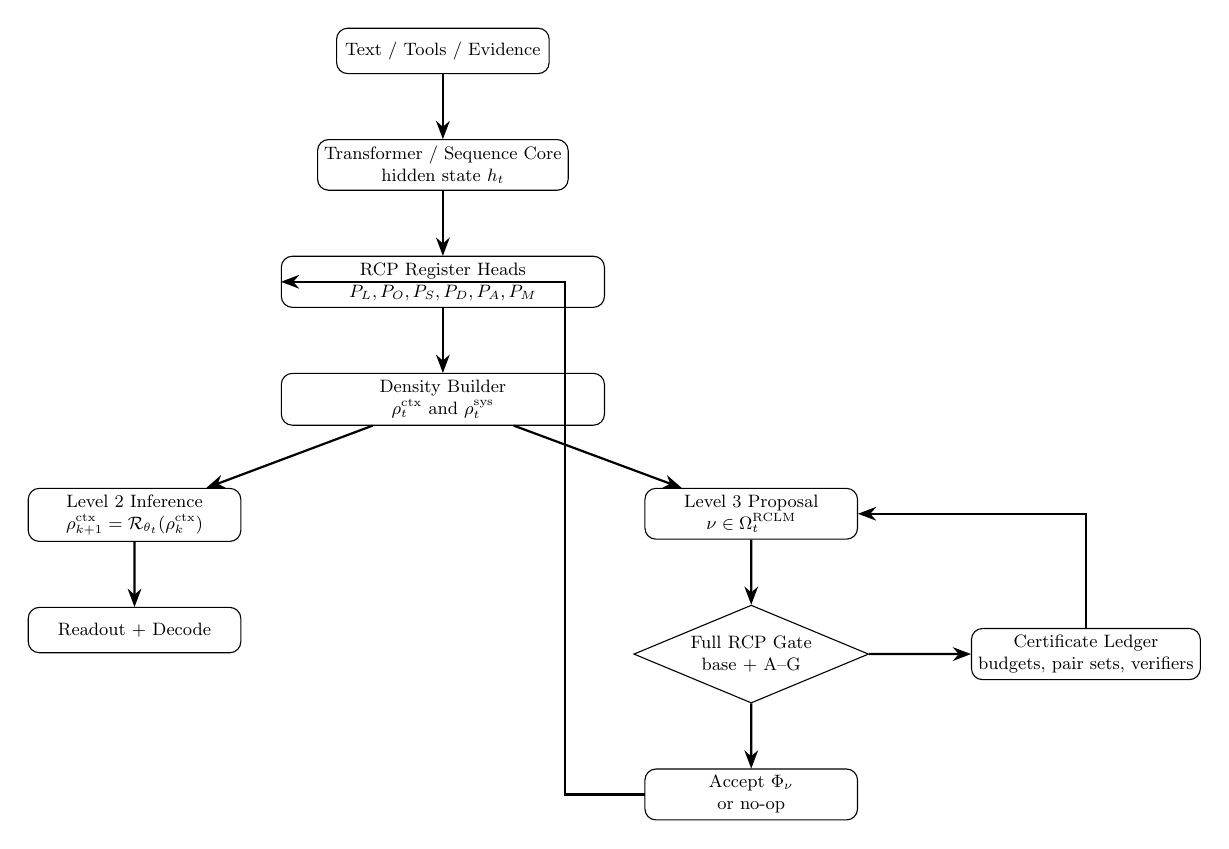
\begin{tikzpicture}[scale=0.72, transform shape,
    node distance=1.15cm and 1.7cm,
    box/.style={rectangle, draw, rounded corners=4pt, minimum width=3.75cm, minimum height=0.8cm, align=center, font=\small},
    wide/.style={rectangle, draw, rounded corners=4pt, minimum width=5.7cm, minimum height=0.9cm, align=center, font=\small},
    gate/.style={diamond, draw, aspect=2.4, align=center, font=\small, inner sep=2pt},
    arrow/.style={->, thick, -{Stealth}}
]
\node[box] (input) {Text / Tools / Evidence};
\node[box, below=of input] (transformer) {Transformer / Sequence Core\\hidden state $h_t$};
\node[wide, below=of transformer] (registers) {RCP Register Heads\\$P_L,P_O,P_S,P_D,P_A,P_M$};
\node[wide, below=of registers] (density) {Density Builder\\$\rho_t^{\ctx}$ and $\rho_t^{\sys}$};
\node[box, below left=1.1cm and 0.7cm of density] (inference) {Level 2 Inference\\$\rho_{k+1}^{\ctx}=\Rcal_{\theta_t}(\rho_k^{\ctx})$};
\node[box, below=of inference] (readout) {Readout + Decode};
\node[box, below right=1.1cm and 0.7cm of density] (proposal) {Level 3 Proposal\\$\nu\in\Omega_t^{\RCLM}$};
\node[gate, below=of proposal] (gate) {Full RCP Gate\\base + A--G};
\node[box, below=of gate] (accept) {Accept $\Phi_\nu$\\or no-op};
\node[box, right=1.8cm of gate] (ledger) {Certificate Ledger\\budgets, pair sets, verifiers};
\draw[arrow] (input) -- (transformer);
\draw[arrow] (transformer) -- (registers);
\draw[arrow] (registers) -- (density);
\draw[arrow] (density) -- (inference);
\draw[arrow] (inference) -- (readout);
\draw[arrow] (density) -- (proposal);
\draw[arrow] (proposal) -- (gate);
\draw[arrow] (gate) -- (accept);
\draw[arrow] (accept.west) -- ++(-1.4,0) |- (registers.west);
\draw[arrow] (gate) -- (ledger);
\draw[arrow] (ledger.north) |- (proposal.east);
\end{tikzpicture}
\caption{RSI--RCLM final v1. The trainable Hamiltonian recursive loop remains Level 2 inference. Level 3 self-modification is admitted only through the full RCP gate.}
\end{figure}


\section{Level 2 Recursive Coherence Inference}

Level 2 is the internal recursive coherence dynamics used during inference.  It operates on context states and does not by itself modify the architecture.  This section expands the dynamics enough to separate density preservation, monitored descent, and convergence claims.

\begin{definition}[Hermitian Hamiltonian parameterization]
For each recursive layer \(l\), let \(A_{t}^{(l)}\) be a complex matrix of trainable parameters.  The corresponding Hermitian Hamiltonian is
\[
H_{\theta_t}^{(l)}=\frac12(A_t^{(l)}+A_t^{(l)\dagger}).
\]
For a step size \(\tau_l\in\mathbb R\), define
\[
U_t^{(l)}=\exp(-iH_{\theta_t}^{(l)}\tau_l).
\]
\end{definition}

\begin{lemma}[Unitary preservation of density states]
\label{lem:unitary-density}
If \(\rho\in\D(\Hcal)\) and \(U\) is unitary, then \(U\rho U^{\dagger}\in\D(\Hcal)\).
\end{lemma}

\begin{proof}
For any vector \(v\), \(v^{\dagger}U\rho U^{\dagger}v=(U^{\dagger}v)^{\dagger}\rho(U^{\dagger}v)\ge0\), so the state is positive semidefinite.  Also \(\Tr(U\rho U^{\dagger})=\Tr(\rho U^{\dagger}U)=\Tr(\rho)=1\).
\end{proof}

\begin{definition}[Spectral coherence projection]
Let \(\rho=Q\operatorname{diag}(\lambda_1,\ldots,\lambda_d)Q^{\dagger}\) with \(\lambda_i\ge0\) and \(\sum_i\lambda_i=1\).  For \(p>0\), define
\[
\operatorname{Pow}_p(\rho)=
\begin{cases}
Q\operatorname{diag}(\lambda_1^p,\ldots,\lambda_d^p)Q^{\dagger}/\sum_i\lambda_i^p,&\sum_i\lambda_i^p>0,\\[0.8em]
I/d,&\sum_i\lambda_i^p=0.
\end{cases}
\]
For a mixing coefficient \(\beta\in[0,1]\), define the mixed projection
\[
\operatorname{Mix}_{p,\beta}(\rho)=(1-\beta)\operatorname{Pow}_p(\rho)+\beta I/d.
\]
\end{definition}

\begin{lemma}[Projection and mixing preserve density states]
\label{lem:projection-density}
If \(\rho\in\D_d\), \(p>0\), and \(\beta\in[0,1]\), then \(\operatorname{Mix}_{p,\beta}(\rho)\in\D_d\).  If \(\beta>0\), then every eigenvalue of \(\operatorname{Mix}_{p,\beta}(\rho)\) is at least \(\beta/d\).
\end{lemma}

\begin{proof}
Eigenvalue powering preserves nonnegativity and normalization after division by \(\sum_i\lambda_i^p\).  Therefore \(\operatorname{Pow}_p(\rho)\) is positive semidefinite and trace one.  A convex combination with \(I/d\) is also positive semidefinite and trace one.  If \(\beta>0\), the eigenvalues of the mixture are \((1-\beta)\mu_i+\beta/d\), where \(\mu_i\ge0\), hence at least \(\beta/d\).
\end{proof}

\begin{definition}[One-step Level 2 inference map]
Given a layer schedule \(l(k)\), exponent \(p_{t,k}>0\), and mixing \(\beta_{t,k}\in[0,1]\), define
\[
\Rcal_{\theta_t,k}(\rho)=
\operatorname{Mix}_{p_{t,k},\beta_{t,k}}
\left(U_t^{(l(k))}\rho U_t^{(l(k))\dagger}\right).
\]
The full internal inference loop is
\[
\rho_{t,k+1}^{\ctx}=\Rcal_{\theta_t,k}(\rho_{t,k}^{\ctx}),
\qquad k=0,1,\ldots,K_t-1.
\]
The halted state is \(\rho_t^{\ctx,*}=\rho_{t,K_t^*}^{\ctx}\), where \(K_t^*\le K_t\) is determined by the halting rule.
\end{definition}

\begin{proposition}[Level 2 density preservation]
\label{prop:level2-density-preservation}
If \(\rho_{t,0}^{\ctx}\in\D(\Hcal_{\RCP})\), then every iterate \(\rho_{t,k}^{\ctx}\) produced by the Level 2 loop is in \(\D(\Hcal_{\RCP})\).
\end{proposition}

\begin{proof}
By Lemma~\ref{lem:unitary-density}, the unitary part maps density states to density states.  By Lemma~\ref{lem:projection-density}, the spectral projection and mixing part maps density states to density states.  Induction over \(k\) proves the claim.
\end{proof}

\begin{definition}[Inference monitor]
The Level 2 monitor is
\[
V_{\mathrm{inf}}(\rho)=
S(\rho)-a_1C_{\ell_1}(\rho)-a_2C_{\rel}(\rho)
+a_3R_{\misgrounded}(\rho)+a_4R_{\collapse}(\rho)+a_5R_{\ambcollapse}(\rho),
\]
with nonnegative coefficients \(a_i\).  The architecture records
\[
\Delta V_{\mathrm{inf},k}=V_{\mathrm{inf}}(\rho_{t,k+1}^{\ctx})-V_{\mathrm{inf}}(\rho_{t,k}^{\ctx}).
\]
\end{definition}

\begin{assumption}[Certified Level 2 descent, when claimed]
A claim of Level 2 stability or convergence is permitted only on a certified domain \(\Xcal_t^{\ctx}\) for which there exist \(\kappa_{\inf}>0\) and \(\eta_{t,k}^{\inf}\ge0\) satisfying
\[
V_{\mathrm{inf}}(\rho_{t,k+1}^{\ctx})
\le
V_{\mathrm{inf}}(\rho_{t,k}^{\ctx})
-\kappa_{\inf}d(\rho_{t,k+1}^{\ctx},\rho_{t,k}^{\ctx})^2
+\eta_{t,k}^{\inf}.
\]
This condition is a certificate assumption, not a consequence of Hamiltonian evolution alone.
\end{assumption}

\begin{theorem}[Conditional Level 2 finite-recursion stability]
\label{thm:level2-finite-stability}
Suppose the certified Level 2 descent assumption holds for \(k=0,\ldots,K-1\).  Then
\[
V_{\mathrm{inf}}(\rho_{t,K}^{\ctx})
\le
V_{\mathrm{inf}}(\rho_{t,0}^{\ctx})
-\kappa_{\inf}\sum_{k=0}^{K-1}d(\rho_{t,k+1}^{\ctx},\rho_{t,k}^{\ctx})^2
+\sum_{k=0}^{K-1}\eta_{t,k}^{\inf}.
\]
In particular,
\[
\sum_{k=0}^{K-1}d(\rho_{t,k+1}^{\ctx},\rho_{t,k}^{\ctx})^2
\le
\frac{V_{\mathrm{inf}}(\rho_{t,0}^{\ctx})-V_{\mathrm{inf}}(\rho_{t,K}^{\ctx})+\sum_{k=0}^{K-1}\eta_{t,k}^{\inf}}{\kappa_{\inf}}.
\]
\end{theorem}

\begin{proof}
Sum the certified descent inequality over \(k=0,\ldots,K-1\).  The left side telescopes, giving the first inequality.  Rearranging gives the second.
\end{proof}

\begin{definition}[Halting rule]
The Level 2 loop halts at the first \(k\le K_t\) satisfying one of the certified stopping conditions:
\[
|\Delta V_{\mathrm{inf},k}|\le\eps_{\halt},
\qquad
d(\rho_{t,k+1}^{\ctx},\rho_{t,k}^{\ctx})\le\delta_{\halt},
\]
or at the hard recursion budget \(K_t\).  The architecture logs whether halting was convergence-based or budget-based.
\end{definition}

\begin{limitation}[No unconditional convergence]
The Level 2 map is density-preserving by construction, but density preservation is not convergence.  Convergence, descent, or improvement claims require the certified descent assumption or another explicit contraction/compactness argument.  This corrects the non-rigorous reading of a recursive Hamiltonian loop as automatically convergent.
\end{limitation}


\section{Level 3 Candidate Self-Improvement}

Level 3 is the self-update channel.  It acts on system-level payloads and may change the architecture that later performs Level 2 inference.  This section expands the dynamics so that \(\Phi_{\nu_t}\) is not confused with \(\Rcal_{\theta_t}\).

\begin{definition}[Self-update candidate code]
A candidate code \(\nu\in\Omega_t^{\RCLM}\) specifies a proposed transformation of some or all of the following components:
\[
\Theta_t,
\quad
\Pcal_t^{\RCLM},
\quad
\{B_{i,t}^{\RCLM}\}_{i\in I_t},
\quad
\{\Gamma_{X,t}\}_{X},
\quad
W_t,
\quad
\mathfrak R_t,
\quad
\Mcal_t,
\quad
\mathcal H_t^{\cert}.
\]
Thus \(\nu\) may update parameters, projections, Hamiltonians, memory, semantic maps, verifier code, barriers, pair-set construction rules, resource estimators, or candidate-generation policies.
\end{definition}

\begin{definition}[Component-level proposed update]
Let \(T_\nu\) be the component-level transformation
\[
T_\nu:\mathcal I_t^{\sys}\mapsto \widetilde{\mathcal I}_{t+1}^{\sys}(\nu).
\]
The corresponding raw successor density is
\[
\widetilde\rho_{t+1}^{\sys}(\nu)=\operatorname{Enc}_{t+1}^{\sys}(\widetilde{\mathcal I}_{t+1}^{\sys}(\nu)).
\]
\end{definition}

\begin{definition}[Accepted self-update channel]
A candidate \(\nu\) induces an accepted self-update channel \(\Phi_\nu\) on the audited state family only when the verifier certifies either:
\begin{enumerate}[label=(\alph*),leftmargin=1.5em]
    \item an exact CPTP representation on that family; or
    \item an approximate implementation with a projection/normalization certificate and an error budget added to every affected RCP inequality.
\end{enumerate}
The accepted successor is
\[
\rho_{t+1}^{\sys}=\Phi_{\nu}(\rho_t^{\sys}).
\]
\end{definition}

\begin{assumption}[No-op and rollback]
The candidate family contains a no-op code \(\nu^0\) satisfying
\[
T_{\nu^0}(\mathcal I_t^{\sys})=\mathcal I_t^{\sys},
\qquad
\Phi_{\nu^0}(\rho_t^{\sys})=\rho_t^{\sys}.
\]
The implementation also maintains a rollback record sufficient to restore the previous payload when a proposed update fails post-application verification.
\end{assumption}

\begin{assumption}[Projection to valid system state]
If a raw candidate produces \(\widetilde\rho_{t+1}^{\sys}\notin\D(\Hcal_{\RCP}\otimes\Hcal_{\arch})\), the candidate is rejected unless a certified projection
\[
\Pi_{\Kcal_{\RCLM,t+1}^{\DG}}(\widetilde\rho_{t+1}^{\sys})\in\Kcal_{\RCLM,t+1}^{\DG}
\]
exists and all projection distortion is included in the RCP gate estimates.
\end{assumption}

\begin{definition}[Raw proposal objective]
A raw candidate may be proposed by an approximate optimizer
\[
\nu_t^{\raw}\in\argmax_{\nu\in\Omega_t^{\RCLM}}
\mathbb E[\mathrm{Perf}_{t+k}\mid \nu,\rho_t^{\sys},M_t],
\]
but raw performance is only a proposal score.  It is not an acceptance criterion.
\end{definition}

\begin{definition}[Accepted update]
The accepted update is selected from the fully augmented RCP--RCLM gate:
\[
\nu_t^*\in\Acal_{\RCP}^{\RCLM\text{-}\DG}(t,\rho_t^{\sys}),
\qquad
\rho_{t+1}^{\sys}=\Phi_{\nu_t^*}(\rho_t^{\sys}).
\]
If no beneficial certified candidate exists, \(\nu_t^*=\nu^0\).
\end{definition}

\begin{proposition}[Level 3 density validity]
\label{prop:level3-density-validity}
Under the system-encoder, accepted-channel, and projection assumptions, every accepted Level 3 update produces a valid system state:
\[
\rho_{t+1}^{\sys}\in\D(\Hcal_{\RCP}\otimes\Hcal_{\arch}).
\]
\end{proposition}

\begin{proof}
If the candidate is certified as an exact accepted channel, density validity follows from the channel certificate.  If the candidate is projected, the projection assumption states that the projected state is in the valid safe set and hence in the density space.  If no beneficial candidate is certified, the no-op leaves \(\rho_t^{\sys}\) unchanged and therefore valid.
\end{proof}

\begin{limitation}[Raw self-editing is not accepted RSI]
A gradient step, architecture rewrite, verifier rewrite, memory edit, or new Hamiltonian proposal is not a valid RSI step merely because it increases predicted performance.  It becomes an accepted RSI--RCLM step only after passing the full post-D--G RCP gate.
\end{limitation}


\section{The Fully Augmented RCP--RCLM Gate}

The RCP gate is the engineering point where the operational-closure math/physics theorem stack attaches to the architecture.  This section defines the gate as a set of checkable residuals rather than only as a symbolic intersection.

\subsection{Base gate}

Let \(\Acal_{\RCP}^{0,\RCLM}(t,\rho_t^{\sys})\) be the set of candidates satisfying the base RCP loss, Lyapunov, barrier, ambiguity, and information-bottleneck conditions:
\[
\Lcal^{\Pcal_t^{\RCLM}}_{\Phi_\nu}\le\eps_t,
\]
\[
\mathbb E[V_{\RCLM}(\Phi_\nu(\rho_t^{\sys}))\mid\rho_t^{\sys}]
\le
V_{\RCLM}(\rho_t^{\sys})-\kappa_Vd(\Phi_\nu(\rho_t^{\sys}),\rho_t^{\sys})^2+\eta_t,
\]
\[
B_{i,t}^{\RCLM}(\Phi_\nu(\rho_t^{\sys}))\le0\quad\forall i\in I_t,
\]
\[
U_t(\nu)\le\zeta_t,
\qquad
I(Z_{t+1};Y_{t+1})\ge I(Z_t;Y_t)-\chi_t.
\]

\subsection{Post-A--C gate}

The post-A--C gate adds constructive recovery, capability and safe-capability control, safe-improvement existence margins, and recursive feasibility.

\begin{definition}[Constructive recovery certificate]
A candidate \(\nu\) supplies a recovery certificate when there exists a recovery map \(\mathcal R_{\Phi_\nu}^{\rec}\) and a recovery error \(r_t\) such that, over the audited safety family \(\Scal_t\),
\[
\sup_{\rho\in\Scal_t}
 d\!\left(\rho,\mathcal R_{\Phi_\nu}^{\rec}(\Phi_\nu(\rho))\right)
\le r_t.
\]
Exact Petz-type recovery is used only under the equality/common-reference hypotheses that justify it. Otherwise recovery is an independently certified architectural object.
\end{definition}

\begin{definition}[Capability functional]
For a task distribution \(\Tcal_t\) and scoring family \(u_\tau\), define
\[
\Cap_t(\rho)=\mathbb E_{\tau\sim\Tcal_t}[u_\tau(\pi_\rho)].
\]
Define safe capability by
\[
\SafeCap_t(\rho)=\Cap_t(\rho)-\lambda_R\Risk_t(\rho).
\]
If the task distribution changes with time, progress claims must specify whether gains are absolute, no-op-normalized, or distribution-shift-normalized.
\end{definition}

\begin{assumption}[Capability--coherence calibration]
For the audited architecture class and task distribution, there exist constants \(a,b,c,d\ge0\) and error \(\omega_t\) such that certified updates satisfy
\[
\Delta\Cap_t(\nu)
\ge
 a\Delta\Ccal_{\RCLM}(\nu)
-b\Lcal^{\Pcal_t^{\RCLM}}_{\Phi_\nu}
-cU_t(\nu)
-dR_{\misgrounded}(\Phi_\nu(\rho_t^{\sys}))
-\omega_t.
\]
This is an empirical or architecture-specific calibration assumption, not a general theorem of information theory.
\end{assumption}

\begin{definition}[Post-A--C gate]
A candidate belongs to \(\Acal_{\RCP}^{\RCLM\text{-}\AC}(t,\rho_t^{\sys})\) when it belongs to the base gate and additionally satisfies:
\begin{enumerate}[label=(\alph*),leftmargin=1.5em]
    \item a recovery certificate with error \(r_t\le r_{\max,t}\);
    \item safe-capability nondegradation or certified progress;
    \item strict residual margins for all active gate constraints when claiming nontrivial improvement;
    \item membership in the current finite- or infinite-horizon viability kernel if a persistent RSI path is claimed.
\end{enumerate}
\end{definition}

\subsection{Post-D--G gate}

The post-D--G gate adds semantic validity, self-model fidelity, verifier bootstrapping, resource feasibility, resource-scaling closure, certificate-inflation control, pair-set coverage-gap control, coherence--capability calibration, residual-specific estimator subprotocol completion, and asymptotic regime conditions. No-op monitoring is treated as a diagnostic policy rather than a hard safety gate, because no-op must remain available when no safe beneficial update can be certified.

\begin{definition}[Semantic interpretation maps]
For each register \(X\in\{L,O,S,D,A,M\}\), the architecture provides
\[
\Gamma_X:\Xcal_X^{\aud}\to\Ycal_X,
\]
where \(\Xcal_X^{\aud}\) is an audited domain of internal states and \(\Ycal_X\) is an externally interpretable semantic space.
\end{definition}

\begin{definition}[Semantic validity]
Let \(x_X^{\true}\in\Ycal_X\) be an externally defined target or audit reference. The semantic error is
\[
\Val_X(\rho)=d_X^{\sem}(\Gamma_X(\rho_X),x_X^{\true}).
\]
The semantic barrier is
\[
B_X^{\sem}(\rho)=\Val_X(\rho)-\delta_X.
\]
Semantic validity requires \(B_X^{\sem}(\rho)\le0\) for all audited registers.
\end{definition}

\begin{definition}[Self-model fidelity]
Let \(M_t^{\mathrm{int}}\) be the self-model encoded in the model and let \(M_t^{\op}\) be the audited operational description of architecture, parameters, objectives, verifier, barriers, limitations, and update effects. Self-model fidelity is
\[
d_M(M_t^{\mathrm{int}},M_t^{\op})\le\epsilon_t^M.
\]
If the audit is only approximately true, an additional audit error term is included.
\end{definition}

\begin{definition}[Verifier state]
The verifier state \(W_t\) includes estimator code, test suites, certificate checkers, semantic audits, pair-set construction procedures, and adversarial search routines. It has soundness \(\Sound(W_t)\) and power \(\Power(W_t)\).
\end{definition}

\begin{definition}[Resource state]
The physical/computational resource state is
\[
\mathfrak R_t=(E_t,K_t,M_t^{\mem},T_t,\Sigma_t,D_t^{\data},V_t^{\val}),
\]
where the entries denote energy, compute, memory, time, entropy/irreversibility budget, data, and validation budget.
\end{definition}

\begin{definition}[Full post-D--G architecture gate]
The final v1 RCP--RCLM gate is
\[
\boxed{%
\begin{aligned}
\Acal_{\RCP}^{\RCLM\text{-}\DG}(t,\rho_t^{\sys})
={}&
\Acal_{\RCP}^{\RCLM\text{-}\AC}(t,\rho_t^{\sys})
\cap \Acal_{\mathrm{type}}(t,\rho_t^{\sys})
\cap \Acal_{\coup}(t,\rho_t^{\sys})\\
&\cap \Acal_{\cert}(t,\rho_t^{\sys})
\cap \Acal_{\trust}(t,\rho_t^{\sys})
\cap \Acal_{\mathrm{tr}}^{\RCLM}(t,\rho_t^{\sys})
\cap \Acal_{\mathrm{proj\mbox{-}real}}^{\RCLM}(t,\rho_t^{\sys})\\
&\cap \Acal_{\cov}(t,\rho_t^{\sys})
\cap \Acal_{\calib}(t,\rho_t^{\sys})
\cap \Acal_{\est}(t,\rho_t^{\sys})
\cap \Acal_{\sem}(t)
\cap \Acal_M(t)
\cap \Acal_{\ver}(t)\\
&\cap \Omega_t^{\phys}
\cap \Acal_{\scale}(t,\rho_t^{\sys};B_t^{\search})
\cap \Acal_{\infl}(t,\rho_t^{\sys}).
\end{aligned}}
\]

Here \(
\Acal_{\cert}\) enforces the audited non-oracular certificate protocol, \(
\Acal_{\trust}\) enforces verifier trust-graph anti-circularity and no self-sole-certification, \(
\Acal_{\cov}\) bounds declared untracked predicate risk, \(
\Acal_{\calib}\) licenses coherence--capability progress claims, \(
\Acal_{\est}\) requires residual-specific estimator subprotocols, \(
\Acal_{\sem}\) enforces semantic validity, \(
\Acal_M\) enforces self-model fidelity, \(
\Acal_{\ver}\) enforces verifier soundness and anti-gaming constraints, \(
\Omega_t^{\phys}\) enforces one-step resource feasibility, \(
\Acal_{\scale}\) enforces audited resource-scaling closure for engine-mode claims, and \(
\Acal_{\infl}\) bounds certificate/budget inflation.  The Batch-3 algebraic non-loss subgate
\[
\Acal_{\RCP}^{\RCLM\text{-}\DG\text{-}\NLalg}
=
\Acal_{\RCP}^{\RCLM\text{-}\DG}\cap\Acal_{\NLalg}^{\RCLM}
\]
is used when the architecture claims that non-loss and recovery are supplied by the certified conservative-extension algebra rather than by direct residual estimation alone.
\end{definition}

\subsection{Synchronization with the operational-closure RCP gate}
\label{subsec:op-rcp-synchronization}

The updated Batch-3 conservative-extension math/physics paper names the abstract operationally closed RCP gate
\[
\Acal_{\RCP}^{\mathrm{op}}(t,\rho_t;g_t^{\min}).
\]
That abstract gate is architecture-general and is now interpreted as part of the Conditional Non-Lossy Self-Update Preservation Theorem rather than as a completed direct RSI engine.  The same reference paper now also defines a conservative-extension non-lossy update algebra; the RCLM-specific version of that algebra is instantiated in Subsection~\ref{subsec:batch3-rclm-conservative-extension-algebra}.  The RSI--RCLM gate above is its RCLM-specific realization.  The purpose of this subsection is only synchronization: it records that the architecture paper has not invented a second safety notion, but has supplied concrete objects for the operational components required by the updated reference paper.

\begin{definition}[RCLM operational instantiation map]
\label{def:rclm-operational-instantiation-map}
An RCLM operational instantiation map at time \(t\) is a bookkeeping map
\[
\mathsf{Inst}_t^{\RCLM}:\Acal_{\RCP}^{\mathrm{op}}(t,\rho_t;g_t^{\min})\leadsto
\Acal_{\RCP}^{\RCLM\text{-}\DG}(t,\rho_t^{\sys})
\]
which assigns the abstract RCP variables to their architecture-level objects:
\[
\rho_t\mapsto \rho_t^{\sys},\qquad
\Phi\mapsto \Phi_\nu,
\qquad
\Pcal_t\mapsto \Pcal_t^{\RCLM},
\]
\[
V\mapsto V_{\RCLM},
\qquad
B_i\mapsto B_{i,t}^{\RCLM},
\qquad
U_t\mapsto U_t^{\RCLM},
\]
\[
(Z_t,Y_t)\mapsto (Z_t^{\RCLM},Y_t^{\RCLM}),
\qquad
\mathfrak q_t\mapsto \mathfrak q_t^{\RCLM},
\qquad
\mathsf{Cert}_t\mapsto \mathsf{Cert}_t^{\RCLM}.
\]
The map is not a new dynamical assumption.  It is a traceability relation between the abstract operational RCP theorem and the concrete RCLM objects defined in this paper.
\end{definition}

\begin{assumption}[Operational synchronization]
\label{ass:rclm-operational-synchronization}
For every accepted candidate \(\nu\), the instantiation map is domain valid and residual preserving in the following conservative sense: each abstract operational residual in \(\Acal_{\RCP}^{\mathrm{op}}\) is either identical to the corresponding RCLM residual or is upper-bounded by the RCLM residual plus an explicitly recorded approximation margin.  Formally, for each abstract residual component \(q_{t,j}^{\mathrm{op}}\) there exists a corresponding architecture residual \(q_{t,k(j)}^{\RCLM}\) and margin \(m_{t,j}^{\mathrm{inst}}\ge0\) such that
\[
q_{t,j}^{\mathrm{op}}(\Phi_\nu)
\le
q_{t,k(j)}^{\RCLM}(\nu)+m_{t,j}^{\mathrm{inst}}.
\]
The margin is included in the relevant certificate radius, budget, or gate threshold.  If no such mapping or bound is certified, the architecture cannot claim that the candidate instantiates the corresponding abstract operational RCP condition.
\end{assumption}

\begin{theorem}[RCLM gate refines the operational RCP gate]
\label{thm:rclm-gate-refines-operational-rcp}
Assume operational synchronization.  If
\[
\nu\in\Acal_{\RCP}^{\RCLM\text{-}\DG}(t,\rho_t^{\sys})
\]
and all instantiation margins are included in the audited certificate radii, then the induced update \(\Phi_\nu\) satisfies the abstract operational RCP gate under the instantiation map:
\[
\Phi_\nu\in
\mathsf{Inst}_t^{\RCLM}\!\bigl(\Acal_{\RCP}^{\mathrm{op}}(t,\rho_t;g_t^{\min})\bigr).
\]
Equivalently, accepted RCLM candidates are conservative architecture-level witnesses for the operationally closed RCP admissibility relation, relative to the declared domains, margins, and certificates.
\end{theorem}

\begin{proof}
Membership in \(\Acal_{\RCP}^{\RCLM\text{-}\DG}\) gives membership in each RCLM component gate: post-A--C, type, coupling, certificate, trust, coverage, calibration, estimator, semantic, self-model, verifier, physical-resource, scaling, and inflation.  By Assumption~\ref{ass:rclm-operational-synchronization}, each corresponding abstract operational residual is bounded by the architecture residual plus a recorded margin.  Since those margins are included in the certificate radii or thresholds, nonpositivity of the certified RCLM residuals implies nonpositivity of the abstract operational residuals.  Therefore the induced \(\Phi_\nu\) satisfies every component of \(\Acal_{\RCP}^{\mathrm{op}}\) represented by the instantiation map.  No conclusion is made about abstract components for which the architecture supplies no domain-valid mapping.
\end{proof}

\begin{limitation}[Synchronization is not extra safety]
The theorem is a traceability theorem, not an additional safety theorem.  It does not make unsafe updates safe.  It only states that, after the math/physics paper introduced \(\Acal_{\RCP}^{\mathrm{op}}\), the already-defined RCLM gate is a conservative concrete refinement of that abstract operational gate.
\end{limitation}

\subsection{Estimator-residual implementation of the gate}

\begin{definition}[Gate residual vector]
For a candidate \(\nu\), define the residual vector
\[
\begin{aligned}
\mathfrak q_t(\nu)=\bigl(&
q_t^{\mathrm{type}},q_t^{\coup},q_t^{\cert},q_t^{\trust},q_t^{\cov},q_t^{\calib},q_t^{\est},
q_t^{\NLalg},q_t^{\loss},q_t^{\rec},q_t^{V},q_t^{B},q_t^{U},q_t^{IB},\\
&
q_t^{\Cap},q_t^{\sem},q_t^M,q_t^{\ver},q_t^{\phys},
q_t^{\scale},q_t^{\infl},q_t^{\asy}
\bigr).
\end{aligned}
\]
where each component is nonpositive exactly when the corresponding gate constraint is satisfied.  For example,
\[
q_t^{\mathrm{type}}(\nu)=0\ \text{if}\ \nu\in\Acal_{\mathrm{type}}(t,\rho_t^{\sys}),\ \text{and}\ >0\ \text{otherwise},
\]
\[
q_t^{\coup}(\nu)=\max_X(\epsilon_{X,t+1}^{\coup}-m_{X,t+1}^{\sem}(\nu)),
\]
\[
q_t^{\cert}(\nu)=0\ \text{if}\ \nu\in\Acal_{\cert}(t,\rho_t^{\sys}),\ \text{and}\ >0\ \text{otherwise},
\]
\[
q_t^{\trust}(\nu)=0\ \text{if}\ \nu\in\Acal_{\trust}(t,\rho_t^{\sys}),\ \text{and}\ >0\ \text{otherwise},
\]
\[
q_t^{\mathrm{tr}}(\nu)=0\ \text{if}\ \nu\in\Acal_{\mathrm{tr}}^{\RCLM}(t,\rho_t^{\sys}),\ \text{and}\ >0\ \text{otherwise},
\]
\[
q_t^{\mathrm{sep}}(\nu)=0\ \text{if}\ \nu\in\Acal_{\mathrm{sep}}^{\RCLM}(t,\rho_t^{\sys}),\ \text{and}\ >0\ \text{otherwise},
\]
\[
q_t^{\mathrm{proj\mbox{-}real}}(\nu)=0\ \text{if}\ \nu\in\Acal_{\mathrm{proj\mbox{-}real}}^{\RCLM}(t,\rho_t^{\sys}),\ \text{and}\ >0\ \text{otherwise},
\]
\[
q_t^{\cov}(\nu)=\operatorname{CovGap}_t(\nu)-\gamma_t^{\cov},
\qquad
q_t^{\calib}(\nu)=e_t^{\cal}(\nu)-e_{\max,t}^{\cal},
\]
\[
q_t^{\est}(\nu)=
\begin{cases}
0, & \text{if all required estimator subprotocols are complete on }\nu,\\
>0, & \text{otherwise,}
\end{cases}
\]
\[
q_t^{\scale}(\nu)=
\begin{cases}
0, & \text{if }\nu\in\Acal_{\scale}(t,\rho_t^{\sys};B_t^{\search}),\\
>0, & \text{otherwise.}
\end{cases}
\]
\[
q_t^{\infl}(\nu)=\operatorname{Infl}_t(\nu)-\iota_t^{\max},
\]

\[
q_t^{\NLalg}(\nu)=
\begin{cases}
0, & \text{if no algebraic non-loss claim is made,}\\
0, & \text{if }\nu\in\Acal_{\NLalg}^{\RCLM}(t,\rho_t^{\sys})\text{ and the claim is made,}\\
>0, & \text{otherwise.}
\end{cases}
\]
\[
q_t^{\loss}(\nu)=\Lcal^{\Pcal_t^{\RCLM}}_{\Phi_\nu}-\eps_t,
\qquad
q_t^{\rec}(\nu)=r_t-r_{\max,t},
\]
\[
q_t^{B}(\nu)=\max_{i\in I_t}B_{i,t}^{\RCLM}(\Phi_\nu(\rho_t^{\sys})),
\qquad
q_t^{\sem}(\nu)=\max_X B_X^{\sem}(\Phi_\nu(\rho_t^{\sys})).
\]
The exact definitions of the remaining residuals are the algebraic left-minus-right forms of their gate inequalities.
\end{definition}

\begin{definition}[One-sided estimator certificate]
An estimator \(\widehat{\mathfrak q}_t\) with error vector \(\Delta_t\ge0\) is one-sided sound on a candidate set \(\Omega_t^{\test}\) when
\[
\mathfrak q_t(\nu)\le \widehat{\mathfrak q}_t(\nu)+\Delta_t
\quad\forall \nu\in\Omega_t^{\test}
\]
with the stated confidence level.  A candidate is accepted only if
\[
\widehat{\mathfrak q}_{t,j}(\nu)+\Delta_{t,j}\le0
\quad\text{for every residual component }j.
\]
\end{definition}

\begin{theorem}[Architecture-level gate soundness]
\label{thm:architecture-gate-soundness}
Assume the one-sided estimator certificate holds for \(\nu\).  If \(\widehat{\mathfrak q}_{t,j}(\nu)+\Delta_{t,j}\le0\) for every residual component \(j\), then \(\nu\in\Acal_{\RCP}^{\RCLM\text{-}\DG}(t,\rho_t^{\sys})\).
\end{theorem}

\begin{proof}
For each component \(j\), one-sided soundness gives \(\mathfrak q_{t,j}(\nu)\le\widehat{\mathfrak q}_{t,j}(\nu)+\Delta_{t,j}\le0\).  By construction of the residual vector, all gate inequalities are therefore satisfied.  Hence \(\nu\) belongs to the intersection defining \(\Acal_{\RCP}^{\RCLM\text{-}\DG}\).
\end{proof}

\begin{definition}[Gate selection objective]
Among certified safe candidates, the architecture may select
\[
\nu_t^*\in\argmax_{\nu\in\Acal_{\RCP}^{\RCLM\text{-}\DG}(t,\rho_t^{\sys})}
\left[
\widehat{\Delta\SafeCap}_t(\nu)-\lambda_{\cost}\widehat C_t^{\tot}(\nu;B_t^{\search})-\lambda_{\infl}\widehat{\operatorname{Infl}}_t(\nu)
\right].
\]
If the feasible set contains no beneficial certified candidate, no-op is selected and the no-op rate monitor is updated.  When the Batch-4 tangent-cone module is enabled, the search procedure may use the projected local direction \(P_{T_{\Acal_t^{\RCLM}}}\nabla_\nu\RSIPot_t\) to propose a small candidate, but the candidate is accepted only after the same certificate, residual, type, trust, resource, and non-loss checks pass. When the Batch-5 engine-viability module is enabled and a recursive engine claim is made, the selected candidate must also be a witness in the appropriate RCLM engine move set \(\mathcal E_t^{\RCLM\text{-}\CE}\) with successor in \(\Vcal_{t+1}^{\RCLM\text{-}\engine,N}\) or \(\Vcal_{t+1}^{\RCLM\text{-}\engine,\infty}\). If the architecture claims an engine-mode improvement rather than merely safe nondegradation, the selected candidate must also belong to the progress-search set \(\Acal_{\mathrm{prog}}(t,\rho_t^{\sys};B_t^{\search})\) defined in Section~\ref{sec:persistent-progress-search}.
\end{definition}

\begin{remark}[No reward for uncertified progress]
A candidate with high predicted capability gain but no recovery certificate, no semantic validity, insufficient resources, or verifier-gaming risk is not admissible.
\end{remark}


\section{Non-Oracular Certification and Audited Estimator Soundness}
\label{sec:non-oracular-certification}

The residual gate above is only useful if its certificates are not treated as hidden perfect oracles. This section specifies an architecture-level certificate construction protocol. It does not prove that all required estimators are easy to build for large trained systems. It replaces an unspecified oracle by explicit audit data, stress tests, coverage assumptions, confidence radii, and a theorem showing when audited estimates imply true one-sided gate satisfaction.

\begin{definition}[Residual index set]
\label{def:residual-index-set}
Let \(\mathcal J_t\) be the finite index set of residual components in \(\mathfrak q_t\). For each \(j\in\mathcal J_t\), the true residual is a map
\[
q_{t,j}:\Omega_t^{\RCLM}\to\mathbb R.
\]
The convention is that \(q_{t,j}(\nu)\le0\) means that the \(j\)-th gate requirement is truly satisfied by \(\nu\). The vector \(\mathfrak q_t(\nu)\) is the ordered collection of these residuals.
\end{definition}

\begin{definition}[Audited candidate domain]
\label{def:audited-candidate-domain}
The audited candidate domain at time \(t\) is a declared subset
\[
\Omega_t^{\aud}\subseteq\Omega_t^{\RCLM}
\]
containing the no-op candidate \(\nu^0\). A candidate outside \(\Omega_t^{\aud}\) is not accepted by the non-oracular gate, even if an uncertified predictor assigns it high capability gain.
\end{definition}

\begin{definition}[Calibration and stress-test packet]
\label{def:calibration-stress-packet}
A calibration and stress-test packet is
\[
\mathsf{Audit}_t
=
(\Dcal_t^{\calib},\Dcal_t^{\hold},\Tcal_t^{\stress},\Ucal_t^{\adv},W_t,\alpha_t),
\]
where \(\Dcal_t^{\calib}\) is calibration data, \(\Dcal_t^{\hold}\) is held-out audit data, \(\Tcal_t^{\stress}\) is a family of stress tests, \(\Ucal_t^{\adv}\) is an adversarial probe family, \(W_t\) is the verifier state, and \(\alpha_t\) records the randomization, split, and access policy used to prevent leakage from the held-out audit process into the proposal generator.
\end{definition}

\begin{definition}[Certificate construction protocol]
\label{def:certificate-construction-protocol}
For \(\nu\in\Omega_t^{\aud}\), a non-oracular certificate packet is
\[
\mathsf{Cert}_t(\nu)
=
\bigl(
\widehat{\mathfrak q}_t(\nu),
\Delta_t^{\aud}(\nu),
\delta_t(\nu),
\mathsf{Audit}_t,
\mathsf{Trace}_t(\nu),
W_t
\bigr).
\]
Here \(\widehat{\mathfrak q}_t(\nu)\) is the estimated residual vector, \(\Delta_t^{\aud}(\nu)\ge0\) is the audited one-sided radius vector, \(\delta_t(\nu)\) is the declared failure probability, and \(\mathsf{Trace}_t(\nu)\) contains estimator versions, data hashes, stress-test identifiers, random seeds or commitments, candidate-generation metadata, and the verifier version used for the decision.
\end{definition}

\begin{assumption}[Audit split and anti-leakage]
\label{ass:audit-split-anti-leakage}
The proposal generator may use training and public calibration information, but it may not adapt to the unrevealed held-out audit outcomes, random stress seeds, or adversarial probe labels used to validate \(\mathsf{Cert}_t(\nu)\). If a candidate modifies the proposal generator, verifier, estimator code, semantic maps, or data-selection process, the certificate must be produced by an independent frozen verifier slice or by a previously certified verifier-transition rule.
\end{assumption}

\begin{assumption}[Audited one-sided residual coverage]
\label{ass:audited-one-sided-coverage}
For each \(j\in\mathcal J_t\), the certificate protocol produces nonnegative radii
\[
\Delta_{t,j}^{\aud}(\nu)
= r_{t,j}^{\calib}(\nu)+r_{t,j}^{\hold}(\nu)+r_{t,j}^{\stress}(\nu)+r_{t,j}^{\adv}(\nu)+r_{t,j}^{\shift}(\nu)
\]
and a failure probability \(\delta_{t,j}\) such that, on an event \(\Ecal_{t,j}^{\cert}\) of probability at least \(1-\delta_{t,j}\),
\[
q_{t,j}(\nu)
\le
\widehat q_{t,j}(\nu)+\Delta_{t,j}^{\aud}(\nu)
\quad
\forall \nu\in\Omega_t^{\aud}.
\]
The radii may be conservative. This assumption is the mathematical form of the empirical claim that the calibration data, held-out audits, stress tests, adversarial probes, and distribution-shift model actually upper-bound the estimator error on the audited candidate domain.
\end{assumption}

\begin{assumption}[Finite simultaneous failure budget]
\label{ass:finite-certificate-failure-budget}
For each finite horizon \(T\), the declared certificate failure budget satisfies
\[
\delta_{0:T}^{\cert}
=
\sum_{t=0}^{T-1}\sum_{j\in\mathcal J_t}\delta_{t,j}<1.
\]
For infinite-horizon claims, the manuscript must explicitly assume \(\sum_{t\ge0}\sum_{j\in\mathcal J_t}\delta_{t,j}<\infty\). No almost-sure or long-horizon soundness conclusion is made without such a summability assumption.
\end{assumption}

\begin{definition}[Non-oracular certificate gate]
\label{def:non-oracular-certificate-gate}
A candidate belongs to \(\Acal_{\cert}(t,\rho_t^{\sys})\) if and only if:
\begin{enumerate}[label=(\roman*),leftmargin=1.5em]
    \item \(\nu\in\Omega_t^{\aud}\);
    \item a complete packet \(\mathsf{Cert}_t(\nu)\) exists;
    \item the audit split and anti-leakage assumptions are satisfied for this candidate;
    \item for every \(j\in\mathcal J_t\),
    \[
    \widehat q_{t,j}(\nu)+\Delta_{t,j}^{\aud}(\nu)\le0.
    \]
\end{enumerate}
This gate is still conditional on the audit-coverage assumptions. It is non-oracular only in the sense that it records how the certificate is constructed and what empirical/statistical assumptions are being used, rather than assuming an unspecified perfect checker.
\end{definition}

\begin{theorem}[One-sided soundness from audited estimators]
\label{thm:audited-one-sided-soundness}
Assume Assumptions~\ref{ass:audit-split-anti-leakage}--\ref{ass:finite-certificate-failure-budget}. Fix a time \(t\). With probability at least
\[
1-\sum_{j\in\mathcal J_t}\delta_{t,j},
\]
every candidate \(\nu\in\Acal_{\cert}(t,\rho_t^{\sys})\) satisfies
\[
q_{t,j}(\nu)\le0
\quad\forall j\in\mathcal J_t.
\]
Consequently, every such candidate satisfies all exact residual inequalities represented by \(\mathfrak q_t\).
\end{theorem}

\begin{proof}
For each residual component \(j\), Assumption~\ref{ass:audited-one-sided-coverage} gives an event \(\Ecal_{t,j}^{\cert}\) with probability at least \(1-\delta_{t,j}\) on which
\[
q_{t,j}(\nu)\le \widehat q_{t,j}(\nu)+\Delta_{t,j}^{\aud}(\nu)
\quad\forall \nu\in\Omega_t^{\aud}.
\]
By the union bound, the intersection \(\Ecal_t^{\cert}=\bigcap_{j\in\mathcal J_t}\Ecal_{t,j}^{\cert}\) has probability at least \(1-\sum_j\delta_{t,j}\). If \(\nu\in\Acal_{\cert}\), then \(\nu\in\Omega_t^{\aud}\) and \(\widehat q_{t,j}(\nu)+\Delta_{t,j}^{\aud}(\nu)\le0\) for all \(j\). On \(\Ecal_t^{\cert}\), therefore, \(q_{t,j}(\nu)\le0\) for all \(j\). This is exactly true residual satisfaction.
\end{proof}

\begin{corollary}[Finite-horizon simultaneous certificate soundness]
\label{cor:finite-horizon-cert-soundness}
If every accepted candidate over times \(0,\ldots,T-1\) belongs to \(\Acal_{\cert}(t,\rho_t^{\sys})\), then all accepted candidates over that horizon satisfy their true residual inequalities with probability at least
\[
1-\sum_{t=0}^{T-1}\sum_{j\in\mathcal J_t}\delta_{t,j}.
\]
\end{corollary}

\begin{proof}
Apply Theorem~\ref{thm:audited-one-sided-soundness} at each time and take a union bound over time and residual components.
\end{proof}

\begin{proposition}[Connection to architecture-level gate soundness]
\label{prop:non-oracular-implies-gate-soundness}
On the simultaneous certificate-validity event of Corollary~\ref{cor:finite-horizon-cert-soundness}, membership in \(\Acal_{\cert}(t,\rho_t^{\sys})\) plus the conservative acceptance rule implies the hypothesis of Theorem~\ref{thm:architecture-gate-soundness}.
\end{proposition}

\begin{proof}
Theorem~\ref{thm:architecture-gate-soundness} requires one-sided residual soundness: \(\mathfrak q_t(\nu)\le \widehat{\mathfrak q}_t(\nu)+\Delta_t\). In the present section, \(\Delta_t\) is instantiated as \(\Delta_t^{\aud}\), and Theorem~\ref{thm:audited-one-sided-soundness} proves exactly the required one-sided relation on the certificate-validity event. The conservative acceptance rule then yields true nonpositivity of every residual.
\end{proof}

\begin{limitation}[Non-oracular does not mean assumption-free]
This section does not prove that the calibration data are representative, that the stress tests are exhaustive, that adversarial probes find every failure mode, or that the radii are tight enough for useful updates to pass. It makes those obligations explicit. If the audit-coverage assumptions fail, the non-oracular certificate theorem does not apply.
\end{limitation}


\section{Verifier Anti-Circularity and Trust-Graph Stability}
\label{sec:verifier-anti-circularity}

The non-oracular certificate protocol still leaves a self-reference risk: an update that changes the verifier, estimator, audit process, semantic map, barrier, or certificate generator might try to certify its own successor.  This section adds an explicit trust-graph layer.  The point is not to prove that a perfect trust anchor exists.  The point is to prevent the architecture theorem from hiding a circular premise.  Verifier-changing candidates are accepted only when their certificate support is independent of the part being changed, or when an already-certified transition rule supplies the needed support.

\begin{definition}[Verifier-relevant component set]
\label{def:verifier-relevant-components}
Let
\[
\mathsf{VRel}_t=
\{W_t,\widehat{\mathfrak q}_t,\Delta_t^{\aud},\mathsf{Audit}_t,\mathsf{Trace}_t,
\Gamma_t,\mathsf B_t,\Pcal_t^{\RCLM},\mathfrak S_t^{\RCLM},\Omega_t^{\aud},\Pi_{\Kcal},\text{proposal generator}\}
\]
be the verifier-relevant components at time \(t\).  For a candidate \(\nu\), let
\[
\operatorname{Aff}_t(\nu)\subseteq \mathsf{VRel}_t
\]
be the set of verifier-relevant components whose code, parameters, data access policy, reference objects, or decision thresholds would be modified by \(\nu\).  If \(\operatorname{Aff}_t(\nu)=\emptyset\), the candidate is not verifier-changing.
\end{definition}

\begin{definition}[Verifier trust graph]
\label{def:verifier-trust-graph}
A verifier trust graph for candidate \(\nu\) at time \(t\) is a finite directed graph
\[
\Gcal_t^{\ver}(\nu)=(\mathsf V_t^{\ver},\mathsf E_t^{\ver},\mathsf A_t^{\anchor},\mathsf T_t(\nu),\mathsf{Ind}_t),
\]
where:
\begin{enumerate}[label=(\roman*),leftmargin=1.5em]
    \item \(\mathsf V_t^{\ver}\) contains verifier nodes, such as frozen verifier slices, independent audit processes, external tests, cross-checker models, hardware-protected ledgers, and previously certified verifier-transition rules;
    \item an edge \(a\to b\) in \(\mathsf E_t^{\ver}\) means that node \(a\) certifies a claim about node \(b\) or about an update affecting \(b\);
    \item \(\mathsf A_t^{\anchor}\subseteq \mathsf V_t^{\ver}\) is the declared set of trust-anchor nodes whose soundness is assumed or externally audited at time \(t\);
    \item \(\mathsf T_t(\nu)\subseteq \mathsf V_t^{\ver}\) is the set of nodes corresponding to the verifier-relevant components affected by \(\nu\);
    \item \(\mathsf{Ind}_t(a,b;\nu)=1\) records that the audit errors, training data, random seeds, held-out tests, and incentives of nodes \(a\) and \(b\) are independent enough for the certificate claim being made about \(\nu\).
\end{enumerate}
The graph is part of the certificate packet and is therefore logged in the certificate ledger.
\end{definition}

\begin{definition}[Trust support set]
\label{def:trust-support-set}
A trust support set for \(\nu\) is a subset
\[
\mathsf{Supp}_t(\nu)\subseteq \mathsf V_t^{\ver}
\]
used to certify the verifier-relevant effects of \(\nu\).  It is called admissible when:
\begin{enumerate}[label=(\alph*),leftmargin=1.5em]
    \item every support node has a directed certification path to each affected verifier-relevant target in \(\mathsf T_t(\nu)\);
    \item no support node lies in \(\mathsf T_t(\nu)\), unless the edge is produced by an already-certified transition rule from an earlier time;
    \item the induced certification subgraph used for \(\nu\) contains no directed cycle in which every node is affected by \(\nu\);
    \item either \(\mathsf{Supp}_t(\nu)\cap\mathsf A_t^{\anchor}\neq\emptyset\), or there exist distinct \(a,b\in\mathsf{Supp}_t(\nu)\) with \(\mathsf{Ind}_t(a,b;\nu)=1\);
    \item all edge claims used by the support set have audited one-sided residual certificates with nonpositive upper bounds.
\end{enumerate}
\end{definition}

\begin{definition}[No self-sole-certification rule]
\label{def:no-self-sole-certification}
A candidate \(\nu\) satisfies the no self-sole-certification rule if either \(\operatorname{Aff}_t(\nu)=\emptyset\), or there exists an admissible trust support set \(\mathsf{Supp}_t(\nu)\) such that the certificate for \(\nu\) is not generated solely by a verifier-relevant component modified by \(\nu\).  Equivalently, verifier-changing updates must be certified by at least one independent support path not contained entirely in the components being rewritten.
\end{definition}

\begin{definition}[Trust-graph residuals]
\label{def:trust-graph-residuals}
The trust-graph residual vector is
\[
\mathfrak r_t^{\trust}(\nu)=
\bigl(r_t^{\graph}(\nu),r_t^{\sole}(\nu),r_t^{\edge}(\nu),r_t^{\sound}(\nu),r_t^{\power}(\nu)\bigr),
\]
where the entries are nonpositive exactly when, respectively, the declared trust graph is well formed, the no self-sole-certification rule holds, all support-edge certificates pass, the successor verifier satisfies the certified soundness degradation bound, and the successor verifier satisfies the certified power-degradation or power-improvement claim.  The aggregate trust residual is
\[
q_t^{\trust}(\nu)=\max\{r_t^{\graph}(\nu),r_t^{\sole}(\nu),r_t^{\edge}(\nu),r_t^{\sound}(\nu),r_t^{\power}(\nu)\}.
\]
\end{definition}

\begin{assumption}[Trust-graph audit soundness]
\label{ass:trust-graph-audit-soundness}
For each audited candidate \(\nu\in\Omega_t^{\aud}\), the trust-graph certificate produces a one-sided radius vector such that, on an event \(\Ecal_t^{\trust}\) of probability at least \(1-\delta_t^{\trust}\), the true trust residual is bounded above by its audited estimate:
\[
q_t^{\trust}(\nu)
\le
\widehat q_t^{\trust}(\nu)+\Delta_t^{\trust}(\nu)
\quad
\forall \nu\in\Omega_t^{\aud}.
\]
This assumption includes the correctness of graph parsing, independence declarations, support-edge audit outcomes, and the claimed relationship between support-edge certificates and verifier soundness/power residuals.  It is not derived from the verifier being updated.
\end{assumption}

\begin{assumption}[Verifier transition degradation budgets]
\label{ass:verifier-transition-budgets}
For accepted verifier-relevant updates, nonpositive trust residuals imply
\[
\Sound(W_{t+1})\ge \Sound(W_t)-\omega_t^{\ver},
\qquad
\Power(W_{t+1})\ge \Power(W_t)-\pi_t^{\ver}.
\]
If the update claims positive verifier-power improvement, the claimed increment must be stated separately and is valid only on the audited task family used to define \(\Power\).  No uniform positive improvement is claimed on a fixed bounded power scale for an unbounded horizon.
\end{assumption}

\begin{definition}[Trust-admissible verifier gate]
\label{def:trust-admissible-verifier-gate}
A candidate belongs to
\[
\Acal_{\trust}(t,\rho_t^{\sys})
\]
if and only if:
\begin{enumerate}[label=(\roman*),leftmargin=1.5em]
    \item \(\nu\in\Omega_t^{\aud}\);
    \item a verifier trust graph \(\Gcal_t^{\ver}(\nu)\) and support set \(\mathsf{Supp}_t(\nu)\) are included in \(\mathsf{Cert}_t(\nu)\);
    \item the no self-sole-certification rule is satisfied;
    \item \(\widehat q_t^{\trust}(\nu)+\Delta_t^{\trust}(\nu)
    \le0\).
\end{enumerate}
If \(\operatorname{Aff}_t(\nu)=\emptyset\), the trust graph may certify that no verifier-relevant component is modified; if \(\operatorname{Aff}_t(\nu)\neq\emptyset\), independent support is required.
\end{definition}

\begin{theorem}[No self-sole-certified verifier update]
\label{thm:no-self-sole-certified-verifier-update}
Assume \(\nu\in\Acal_{\trust}(t,\rho_t^{\sys})\).  If \(\operatorname{Aff}_t(\nu)\neq\emptyset\), then the acceptance certificate for \(\nu\) includes an admissible support set that is not contained entirely in the components modified by \(\nu\).  Therefore \(\nu\) is not accepted solely on the authority of the verifier component it rewrites.
\end{theorem}

\begin{proof}
By Definition~\ref{def:trust-admissible-verifier-gate}, membership in \(\Acal_{\trust}\) requires a trust graph, a support set, and satisfaction of the no self-sole-certification rule.  By Definition~\ref{def:no-self-sole-certification}, a verifier-changing candidate must have at least one independent support path not contained entirely in the affected verifier-relevant components.  Hence sole self-certification is excluded by construction.
\end{proof}

\begin{theorem}[Verifier self-consistency stability]
\label{thm:verifier-self-consistency-stability}
Let \(\nu_0,\ldots,\nu_{T-1}\) be accepted candidates with \(\nu_t\in\Acal_{\trust}(t,\rho_t^{\sys})\).  Assume the trust-graph audit soundness events \(\Ecal_t^{\trust}\) hold for all \(t<T\), and assume the verifier transition degradation budgets of Assumption~\ref{ass:verifier-transition-budgets}.  Then:
\begin{enumerate}[label=(\roman*),leftmargin=1.5em]
    \item no verifier-changing accepted update over the horizon is sole-self-certified;
    \item verifier soundness satisfies
    \[
    \Sound(W_T)\ge \Sound(W_0)-\sum_{t=0}^{T-1}\omega_t^{\ver};
    \]
    \item verifier power satisfies
    \[
    \Power(W_T)\ge \Power(W_0)-\sum_{t=0}^{T-1}\pi_t^{\ver}.
    \]
\end{enumerate}
\end{theorem}

\begin{proof}
Item (i) follows by applying Theorem~\ref{thm:no-self-sole-certified-verifier-update} at each time \(t<T\).  On the trust-soundness event, \(\nu_t\in\Acal_{\trust}\) gives \(q_t^{\trust}(\nu_t)\le0\), so the soundness and power residuals are nonpositive.  By Assumption~\ref{ass:verifier-transition-budgets},
\[
\Sound(W_{t+1})\ge \Sound(W_t)-\omega_t^{\ver},
\qquad
\Power(W_{t+1})\ge \Power(W_t)-\pi_t^{\ver}.
\]
Telescoping the first inequality from \(0\) to \(T-1\) yields item (ii), and telescoping the second yields item (iii).
\end{proof}

\begin{corollary}[Probabilistic finite-horizon trust soundness]
\label{cor:finite-horizon-trust-soundness}
If \(\Pr(\Ecal_t^{\trust})\ge1-\delta_t^{\trust}\), then the conclusions of Theorem~\ref{thm:verifier-self-consistency-stability} hold with probability at least
\[
1-
\sum_{t=0}^{T-1}\delta_t^{\trust},
\]
provided the non-oracular certificate-validity events used in Section~\ref{sec:non-oracular-certification} also hold.
\end{corollary}

\begin{proof}
Apply the union bound to the events \(\Ecal_t^{\trust}\) and then condition on the simultaneous non-oracular certificate-validity events.  On that intersection, the deterministic hypotheses of Theorem~\ref{thm:verifier-self-consistency-stability} are satisfied.
\end{proof}

\begin{limitation}[Trust graphs are not magic trust]
The trust graph does not create soundness from nothing.  It prevents a verifier from being the sole certifier of its own successor under the stated graph and independence assumptions.  The existence of externally valid anchors, independent support, representative stress tests, and conservative radii remains an architecture and implementation obligation.
\end{limitation}



\section{Batch-10 Adaptive-Audit Trust and Common-Mode Risk Gate}
\label{sec:batch10-adaptive-audit-trust}

The trust graph in Section~\ref{sec:verifier-anti-circularity} prevents the simplest circularity: a verifier-changing update cannot be certified solely by the verifier component it rewrites.  A realistic adaptive system can still fail through correlated verifier errors, shared training data, public stress-test overfitting, audit leakage, collusive support nodes, or common-mode blind spots.  This section adds an adversarial audit layer.  It does not prove that independent verifiers exist; it defines the additional certificates required before the architecture may claim robustness against adaptive verifier gaming.

\begin{definition}[Correlated verifier failure]
\label{def:corrfail-rclm}
For verifier or audit nodes \(W_i,W_j\in\mathsf V_t^{\ver}\), let
\[
\CorrFail_t(W_i,W_j)\in[0,1]
\]
be an audited upper bound on the probability or normalized risk that \(W_i\) and \(W_j\) fail on the same candidate family because of shared data, shared architecture, shared reward model, shared blind spot, common implementation dependency, or common adversarial pressure.  The value is not inferred from graph distinctness alone; it must be estimated, bounded, or externally audited.
\end{definition}

\begin{definition}[Audit leakage risk]
\label{def:audit-leak-rclm}
For a candidate \(\nu\), define
\[
\AuditLeak_t(\nu)\in[0,1]
\]
as an audited upper bound on the risk that \(\nu\), its proposal generator, or a verifier component affected by \(\nu\) had improper access to held-out audit labels, unrevealed random stress seeds, adversarial probe labels, private red-team prompts, or post-selection evaluation outcomes before the certificate was produced.
\end{definition}

\begin{definition}[Common-mode and collusion risk]
\label{def:common-mode-collusion-rclm}
For a trust support set \(\mathsf{Supp}_t(\nu)\), define the common-mode risk
\[
\CommonMode_t(\mathsf{Supp}_t(\nu))
=
\max\left\{
\sup_{i\ne j\in\mathsf{Supp}_t(\nu)}\CorrFail_t(W_i,W_j),
\widehat C_t^{\mathrm{shared}}(\mathsf{Supp}_t(\nu))
\right\},
\]
where \(\widehat C_t^{\mathrm{shared}}\) is an audited shared-dependency score.  Define the collusion risk
\[
\CollusionRisk_t(\mathsf{Supp}_t(\nu))\in[0,1]
\]
as an audited upper bound on the risk that the support nodes are not decision-independent because of common control, incentives, communication, model-merging, shared hidden state, or candidate-induced coordination.
\end{definition}

\begin{definition}[Adaptive trust thresholds]
\label{def:adaptive-trust-thresholds}
Let
\[
\gamma_t^{\mathrm{corr}},\qquad
\gamma_t^{\mathrm{leak}},\qquad
\gamma_t^{\mathrm{cm}},\qquad
\gamma_t^{\mathrm{coll}}
\]
be the maximum accepted correlated-failure, audit-leakage, common-mode, and collusion risks.  These thresholds are gate parameters and must be recorded in the certificate ledger.  Tightening or relaxing them is a verifier/gate-affecting update and must itself satisfy the trust gate.
\end{definition}

\begin{definition}[Adaptive-audit certificate]
\label{def:adaptive-audit-certificate}
An adaptive-audit certificate for \(\nu\) is
\[
\begin{aligned}
\mathsf{AdvAudit}_t(\nu)=(&\widehat{\CorrFail}_t,\widehat{\AuditLeak}_t,
\widehat{\CommonMode}_t,\\
&\widehat{\CollusionRisk}_t,
\Delta_t^{\advtrust},\delta_t^{\advtrust},
\mathsf{AuditIndTrace}_t).
\end{aligned}
\]
where \(\Delta_t^{\advtrust}\) is a vector of one-sided radii, \(\delta_t^{\advtrust}\) is the failure probability, and \(\mathsf{AuditIndTrace}_t\) records data-lineage, held-out split, stress-test secrecy, verifier-dependency, and support-node independence evidence.
\end{definition}

\begin{assumption}[Adaptive-audit one-sided soundness]
\label{ass:adaptive-audit-one-sided-soundness}
For every audited candidate \(\nu\in\Omega_t^{\aud}\), with probability at least \(1-\delta_t^{\advtrust}\), the true adaptive trust risks are bounded by their audited estimates plus radii:
\[
\CorrFail_t(W_i,W_j)
\le
\widehat{\CorrFail}_t(W_i,W_j)+\Delta_{t,ij}^{\mathrm{corr}},
\]
\[
\AuditLeak_t(\nu)
\le
\widehat{\AuditLeak}_t(\nu)+\Delta_t^{\mathrm{leak}},
\]
\[
\CommonMode_t(\mathsf{Supp}_t(\nu))
\le
\widehat{\CommonMode}_t(\mathsf{Supp}_t(\nu))+\Delta_t^{\mathrm{cm}},
\]
\[
\CollusionRisk_t(\mathsf{Supp}_t(\nu))
\le
\widehat{\CollusionRisk}_t(\mathsf{Supp}_t(\nu))+\Delta_t^{\mathrm{coll}}.
\]
This is an empirical/audit assumption, not a theorem implied by graph topology.
\end{assumption}

\begin{definition}[Adaptive trust gate]
\label{def:adaptive-trust-gate-rclm}
A candidate belongs to the adaptive trust gate
\[
\Acal_{\trust}^{\adv}(t,\rho_t^{\sys})
\]
when all of the following hold:
\begin{enumerate}[label=(\roman*),leftmargin=1.5em]
    \item \(\nu\in\Acal_{\trust}(t,\rho_t^{\sys})\);
    \item \(\mathsf{AdvAudit}_t(\nu)\) is present in the certificate packet;
    \item for all distinct \(W_i,W_j\in\mathsf{Supp}_t(\nu)\),
    \[
    \widehat{\CorrFail}_t(W_i,W_j)+\Delta_{t,ij}^{\mathrm{corr}}\le\gamma_t^{\mathrm{corr}};
    \]
    \item
    \[
    \widehat{\AuditLeak}_t(\nu)+\Delta_t^{\mathrm{leak}}\le\gamma_t^{\mathrm{leak}};
    \]
    \item
    \[
    \widehat{\CommonMode}_t(\mathsf{Supp}_t(\nu))+\Delta_t^{\mathrm{cm}}\le\gamma_t^{\mathrm{cm}};
    \]
    \item
    \[
    \widehat{\CollusionRisk}_t(\mathsf{Supp}_t(\nu))+\Delta_t^{\mathrm{coll}}\le\gamma_t^{\mathrm{coll}}.
    \]
\end{enumerate}
\end{definition}

\begin{definition}[Adaptive trust residual]
\label{def:adaptive-trust-residual-rclm}
Define
\[
\begin{aligned}
q_t^{\trustadv}(\nu)=\max\Bigl\{&
\sup_{i\ne j\in\mathsf{Supp}_t(\nu)}
(\CorrFail_t(W_i,W_j)-\gamma_t^{\mathrm{corr}}),\\
&\AuditLeak_t(\nu)-\gamma_t^{\mathrm{leak}},\\
&\CommonMode_t(\mathsf{Supp}_t(\nu))-\gamma_t^{\mathrm{cm}},\\
&\CollusionRisk_t(\mathsf{Supp}_t(\nu))-\gamma_t^{\mathrm{coll}}
\Bigr\}.
\end{aligned}
\]
The residual is nonpositive exactly when the adaptive-audit risk thresholds are satisfied.
\end{definition}

\begin{theorem}[Adaptive-audit trust soundness]
\label{thm:adaptive-audit-trust-soundness}
Assume adaptive-audit one-sided soundness.  If
\[
\nu\in\Acal_{\trust}^{\adv}(t,\rho_t^{\sys}),
\]
then, on the adaptive-audit soundness event,
\[
q_t^{\trustadv}(\nu)
\le0.
\]
Consequently, if \(\nu\) is verifier-changing, it is not solely self-certified and its correlated-failure, audit-leakage, common-mode, and collusion risks are bounded by their declared thresholds.
\end{theorem}

\begin{proof}
Membership in \(\Acal_{\trust}^{\adv}\) implies membership in \(\Acal_{\trust}\), so Theorem~\ref{thm:no-self-sole-certified-verifier-update} excludes sole self-certification for verifier-changing candidates.  The same membership also gives the four conservative audited inequalities in Definition~\ref{def:adaptive-trust-gate-rclm}.  On the adaptive-audit soundness event, each true risk is bounded above by its audited estimate plus radius.  Therefore every term in the maximum defining \(q_t^{\trustadv}\) is nonpositive, proving the residual bound and the declared risk bounds.
\end{proof}

\begin{corollary}[Finite-horizon adaptive-trust accounting]
\label{cor:finite-horizon-adaptive-trust}
If accepted verifier-relevant updates satisfy \(\nu_t\in\Acal_{\trust}^{\adv}(t,\rho_t^{\sys})\) for \(t<T\), then the adaptive trust bounds hold for all accepted verifier-relevant updates over the horizon with probability at least
\[
1-\sum_{t=0}^{T-1}\delta_t^{\advtrust},
\]
intersected with the ordinary trust-graph and non-oracular certificate-validity events.
\end{corollary}

\begin{limitation}[Adaptive trust remains empirical]
The adaptive trust gate is stronger than no self-sole-certification, but it still depends on audit quality.  If all support nodes share an unmodeled blind spot, if leakage is undetected, or if collusion risk is underestimated, the theorem does not apply.  The module makes adaptive-audit assumptions explicit; it does not create independent trust anchors from notation.
\end{limitation}

\section{Persistent Progress and Budgeted Certified Search}
\label{sec:persistent-progress-search}

The preceding gate can certify safety-preserving self-updates.  A safe filter, however, is not yet an RSI engine.  To move from ``reject unsafe changes'' toward ``find safe beneficial changes,'' the architecture needs a separate progress/search layer.  This layer does not weaken the RCP gate.  It defines when the architecture is allowed to claim nontrivial progress, and what assumptions are needed for a finite-budget search process to find such a candidate.

\begin{remark}[Safety gate versus engine-mode progress gate]
The safety gate admits no-op and safe nondegrading candidates.  The engine-mode progress gate is used only when the architecture claims a nontrivial RSI improvement.  If the progress gate is empty, the architecture must select no-op or defer self-modification; it may not relax safety constraints to force progress.  This distinction prevents no-op fallback from being misrepresented as capability progress and prevents benchmark relabeling from being treated as an improvement theorem.
\end{remark}

\begin{definition}[Safety-admissible candidate set]
\label{def:safety-admissible-candidate-set}
The safety-admissible candidate set at time \(t\) is
\[
\Acal_t^{\safe}(\rho_t^{\sys})
:=
\Acal_{\RCP}^{\RCLM\text{-}\DG}(t,\rho_t^{\sys}).
\]
This set includes no-op whenever the standing no-op feasibility, type, coupling, certificate, trust, semantic, self-model, verifier, and resource assumptions are satisfied by no-op.  Membership in \(\Acal_t^{\safe}\) is a safety statement, not a progress statement.
\end{definition}

\begin{definition}[No-op-normalized safe-capability increment]
\label{def:no-op-normalized-safe-capability-increment}
Let \(\nu_t^0\) denote the certified no-op candidate.  For a candidate \(\nu\), define
\[
\Delta\SafeCap_t^{0}(\nu)
=
\SafeCap_{t+1}\!\left(\Phi_\nu(\rho_t^{\sys})\right)
-
\SafeCap_{t+1}\!\left(\Phi_{\nu_t^0}(\rho_t^{\sys})\right).
\]
The right-hand side evaluates both the candidate and no-op on the same successor-time scoring convention \(\SafeCap_{t+1}\).  Thus a positive value cannot be obtained merely by changing the task distribution between \(t\) and \(t+1\).  This quantity is equal to \(G_t^{\mathrm{noop}}(\nu)\) from Definition~\ref{def:noop-normalized-improvement}, when that definition is invoked later in the Modules A--C section.
\end{definition}

\begin{definition}[Beneficial safe-improvement set]
\label{def:beneficial-safe-improvement-set}
Let \(\epsilon_t^{\mathrm{prog}}>0\) be the progress threshold at time \(t\).  The beneficial safe-improvement set is
\[
\boxed{
\mathcal I_t
=
\left\{
\nu\in\Acal_t^{\safe}(\rho_t^{\sys})
:
\Delta\SafeCap_t^{0}(\nu)>\epsilon_t^{\mathrm{prog}}
\right\}.
}
\]
The threshold \(\epsilon_t^{\mathrm{prog}}\) is distinct from the relative-entropy loss budget \(\eps_t\).  A candidate in \(\mathcal I_t\) is both safe-admissible and no-op-normalized beneficial.  The architecture may claim a nontrivial RSI step at time \(t\) only if the selected candidate belongs to \(\mathcal I_t\) or to a certified conservative subset of it.
\end{definition}

\begin{definition}[Margin-strengthened beneficial set]
\label{def:margin-strengthened-beneficial-set}
For a safety margin \(m_t^{\safe}>0\) and a progress margin \(m_t^{\mathrm{prog}}>0\), let
\[
\mathcal I_t^{m}
=
\left\{
\nu\in\Omega_t^{\aud}:
\mathfrak q_{t,j}(\nu)\le -m_t^{\safe}\ \forall j\in\mathcal J_t,
\quad
\Delta\SafeCap_t^{0}(\nu)\ge \epsilon_t^{\mathrm{prog}}+m_t^{\mathrm{prog}}
\right\}.
\]
This set is not directly observable in large learned systems.  It is the true target set that a conservative audited search procedure attempts to discover.
\end{definition}

\begin{definition}[Budgeted candidate search]
\label{def:budgeted-candidate-search}
A budgeted search procedure is a map
\[
\mathsf{Search}_t(B_t^{\search},\rho_t^{\sys},W_t)
=
S_t(B_t^{\search})\subseteq\Omega_t^{\aud},
\]
where \(B_t^{\search}\) is a declared search budget measured in compute, validation calls, memory, time, data, and verifier invocations.  The search output is finite.  Every candidate returned by the search must still pass the non-oracular certificate gate and trust-graph gate before being accepted.
\end{definition}

\begin{definition}[Certified progress-search gate]
\label{def:certified-progress-search-gate}
Let \(\widehat G_t^{0}(\nu)\) be an estimator of \(\Delta\SafeCap_t^{0}(\nu)\), and let \(\Delta_t^{G}(\nu)\ge0\) be a one-sided lower-bound radius satisfying the soundness condition stated below.  The certified progress-search gate is
\[
\Acal_{\mathrm{prog}}(t,\rho_t^{\sys};B_t^{\search})
=
\left\{
\nu\in S_t(B_t^{\search})\cap\Acal_t^{\safe}(\rho_t^{\sys}):
\widehat G_t^{0}(\nu)-\Delta_t^{G}(\nu)>\epsilon_t^{\mathrm{prog}}
\right\}.
\]
A candidate in this set has a conservative audited certificate of positive no-op-normalized safe-capability gain, provided the gain-estimator event below holds.
\end{definition}

\begin{assumption}[One-sided gain-estimator soundness]
\label{ass:one-sided-gain-estimator-soundness}
For each audited candidate \(\nu\in\Omega_t^{\aud}\), there is an event \(\Ecal_t^{G}\) of probability at least \(1-\delta_t^G\) on which
\[
\Delta\SafeCap_t^{0}(\nu)
\ge
\widehat G_t^{0}(\nu)-\Delta_t^{G}(\nu)
\quad
\forall \nu\in\Omega_t^{\aud}.
\]
The radius \(\Delta_t^G\) must include calibration error, held-out evaluation error, distribution-shift error, adversarial-test error, and scoring-model uncertainty.  No progress claim is made outside the audited domain.
\end{assumption}

\begin{assumption}[Certified search completeness with budget]
\label{ass:certified-search-completeness-budget}
For each time \(t\), budget \(B_t^{\search}\), and audited domain \(\Omega_t^{\aud}\), there is a failure probability \(\delta_t^{\search}\) such that, on an event \(\Ecal_t^{\search}\) of probability at least \(1-\delta_t^{\search}\), the following implication holds:
\[
\mathcal I_t^{m}\neq\emptyset
\quad\Longrightarrow\quad
\exists \nu\in S_t(B_t^{\search})
\]
such that the candidate has complete conservative certificates satisfying
\[
\widehat{\mathfrak q}_{t,j}(\nu)+\Delta_{t,j}^{\aud}(\nu)\le0
\quad\forall j\in\mathcal J_t,
\qquad
\widehat G_t^{0}(\nu)-\Delta_t^{G}(\nu)>
\epsilon_t^{\mathrm{prog}}.
\]
This is stronger than merely searching a neighborhood: it is a search-and-certification completeness assumption for margin-qualified useful candidates.  It is not a theorem from RCP alone.  It may be justified in an implementation by exhaustive enumeration over a finite candidate class, branch-and-bound with certified pruning, randomized search with a coverage bound plus calibrated confidence sequences, or an externally audited search-completeness certificate.  The assumption fails if the budget is too small, if the candidate class excludes the useful update, if the estimator is too pessimistic to certify a truly useful candidate, or if the search procedure can be adversarially steered away from the useful region.
\end{assumption}

\begin{assumption}[Persistent improvement condition]
\label{ass:persistent-improvement-condition-rclm}
For a declared engine horizon \(T\) and times \(t<T\), suppose the state lies in an engine-viability region \(\Vcal_t^{\mathrm{eng}}\subseteq\Kcal_{\RCLM,t}^{\DG}\) and the resource state satisfies a search-feasibility condition
\[
\mathfrak R_t\succeq 
\mathfrak R_{\min,t}^{\search}.
\]
The persistent improvement condition states that
\[
\rho_t^{\sys}\in\Vcal_t^{\mathrm{eng}}
\quad\Longrightarrow\quad
\mathcal I_t^{m}\neq\emptyset.
\]
This is the architecture-level existence premise needed to treat the system as an engine rather than only as a safety filter.  It is not derived from Lyapunov stability, relative-entropy non-loss, or semantic validity alone.
\end{assumption}

\begin{definition}[Engine-mode admissibility]
\label{def:engine-mode-admissibility}
The engine-mode admissible set is
\[
\Acal_{\mathrm{eng}}(t,\rho_t^{\sys};B_t^{\search})
=
\Acal_{\mathrm{prog}}(t,\rho_t^{\sys};B_t^{\search}).
\]
The architecture may still choose no-op from \(\Acal_t^{\safe}\) when \(\Acal_{\mathrm{eng}}\) is empty, but it may not describe that no-op as a nontrivial RSI improvement.  Thus the safety gate and the engine-mode progress gate play different logical roles.
\end{definition}

\begin{theorem}[Budgeted search finds certified beneficial updates under stated assumptions]
\label{thm:budgeted-search-finds-beneficial-updates}
Assume at time \(t\):
\begin{enumerate}[label=(\alph*),leftmargin=1.5em]
    \item the one-sided certificate events for the safety residuals hold;
    \item the gain-estimator event \(\Ecal_t^G\) holds;
    \item the search-completeness event \(\Ecal_t^{\search}\) holds;
    \item \(\mathcal I_t^{m}\neq\emptyset\).
\end{enumerate}
Then \(\Acal_{\mathrm{prog}}(t,\rho_t^{\sys};B_t^{\search})\neq\emptyset\).  Any candidate \(\nu\in\Acal_{\mathrm{prog}}\) satisfies
\[
\nu\in\Acal_t^{\safe}(\rho_t^{\sys})
\quad\text{and}\quad
\Delta\SafeCap_t^{0}(\nu)>\epsilon_t^{\mathrm{prog}}
\]
on the stated certificate-validity events.
\end{theorem}

\begin{proof}
By Assumption~\ref{ass:certified-search-completeness-budget} and \(\mathcal I_t^m\neq\emptyset\), there exists a searched candidate \(\nu\in S_t(B_t^{\search})\) whose conservative safety residuals satisfy
\[
\widehat{\mathfrak q}_{t,j}(\nu)+\Delta_{t,j}^{\aud}(\nu)\le0
\quad\forall j\in\mathcal J_t
\]
and whose conservative no-op-normalized gain certificate satisfies
\[
\widehat G_t^{0}(\nu)-\Delta_t^G(\nu)>
\epsilon_t^{\mathrm{prog}}.
\]
The first display, together with the one-sided residual soundness event, implies \(\nu\in\Acal_t^{\safe}(\rho_t^{\sys})\).  The second display and Assumption~\ref{ass:one-sided-gain-estimator-soundness} imply
\[
\Delta\SafeCap_t^{0}(\nu)
\ge
\widehat G_t^{0}(\nu)-\Delta_t^{G}(\nu)
>
\epsilon_t^{\mathrm{prog}}.
\]
Thus \(\nu\in\Acal_{\mathrm{prog}}(t,\rho_t^{\sys};B_t^{\search})\), proving nonemptiness and the stated safety/progress properties.  The proof uses the explicit search-and-certification completeness hypothesis; it does not infer a conservative certificate merely from true usefulness.
\end{proof}

\begin{corollary}[Finite-horizon engine progress]
\label{cor:finite-horizon-engine-progress}
Fix a finite horizon \(T\).  Suppose the persistent improvement condition holds for all \(t<T\), the search and certificate events in Theorem~\ref{thm:budgeted-search-finds-beneficial-updates} hold for all \(t<T\), and the selected candidate \(\nu_t^*\in\Acal_{\mathrm{prog}}(t,\rho_t^{\sys};B_t^{\search})\) whenever the engine-mode set is nonempty.  Then, with probability at least
\[
1-
\sum_{t=0}^{T-1}
\left(\delta_t^{G}+\delta_t^{\search}+\sum_{j\in\mathcal J_t}\delta_{t,j}+\delta_t^{\trust}\right),
\]
all selected non-no-op engine-mode updates over the horizon are safety-admissible and satisfy
\[
\Delta\SafeCap_t^{0}(\nu_t^*)>\epsilon_t^{\mathrm{prog}}.
\]
If, in addition, the scoring convention is fixed over the horizon or explicitly no-op-normalized at each step, then the safe-capability gains telescope according to the conditional safe-capability theorem in Module B.
\end{corollary}

\begin{proof}
Apply Theorem~\ref{thm:budgeted-search-finds-beneficial-updates} at each time and union bound over gain, search, residual-certificate, and trust-soundness failure events.  The telescope statement is exactly the finite-horizon safe-capability telescope applied to the one-step gains certified here.  No infinite-horizon or fixed-scale uniform progress conclusion follows.
\end{proof}

\begin{limitation}[Progress remains conditional]
\label{lim:persistent-progress-conditional}
This section turns persistent progress into a precise condition and gives a theorem showing how budgeted search can find a beneficial safe update under that condition.  It does not prove that \(\mathcal I_t\) is nonempty for arbitrary RCLM architectures, that the search budget scales favorably, or that useful safe-improvement neighborhoods persist indefinitely.  Those claims require implementation-specific construction, empirical calibration, and the resource-scaling/no-op-pressure controls of Section~\ref{sec:resource-noop-pressure}.
\end{limitation}

\section{Resource-Scaling Closure and No-Op Pressure Control}
\label{sec:resource-noop-pressure}

The progress-search theorem of Section~\ref{sec:persistent-progress-search} still leaves two practical failure modes. First, certification may become more expensive than the useful update it is meant to validate. Second, no-op fallback can become a stable equilibrium, or the system may respond by loosening certificates in order to escape stagnation. This section adds an explicit resource-scaling closure condition, a no-op-rate monitor, and a certificate-inflation penalty. These mechanisms do not prove that frontier-scale certification is cheap. They state the exact assumptions under which the architecture may claim that progress search remains resource-feasible without silently relaxing the safety gate.

\begin{remark}[Why this is not a scalability theorem from first principles]
The RCP theorem stack gives conditional preservation once admissible updates are selected. It does not imply that all residuals can be estimated at low cost, that candidate search is polynomial, or that verification costs are sublinear in system size. The present section therefore treats resource scaling as an additional audited condition, not as a consequence of Lyapunov stability or relative-entropy non-loss.
\end{remark}

\begin{definition}[Architecture cost accounts]
\label{def:architecture-cost-accounts}
For a candidate update \(\nu\) and search budget \(B_t^{\search}\), define nonnegative cost accounts
\[
C_t^{\search}(B_t^{\search}),\quad
C_t^{\cert}(\nu),\quad
C_t^{\verify}(\nu),\quad
C_t^{\rec}(\nu),\quad
C_t^{\apply}(\nu),\quad
C_t^{\rollback}(\nu),\quad
C_t^{\aud}(\nu).
\]
The total certification-and-application cost is
\[
\begin{aligned}
C_t^{\tot}(\nu;B_t^{\search})
={}&
C_t^{\search}(B_t^{\search})+C_t^{\cert}(\nu)+C_t^{\verify}(\nu)+C_t^{\rec}(\nu)\\
&+C_t^{\apply}(\nu)+C_t^{\rollback}(\nu)+C_t^{\aud}(\nu).
\end{aligned}
\]
Let
\[
R_t^{\avail}:=\Budget(\mathfrak R_t)
\]
be the scalar budget extracted from the resource state. This scalar may be a conservative normalized aggregate of energy, compute, memory, time, validation data, and irreversibility budget.
\end{definition}

\begin{assumption}[Audited cost upper bounds]
\label{ass:audited-cost-upper-bounds}
For each accepted candidate, the architecture supplies an audited cost estimate \(\widehat C_t^{\tot}(\nu;B_t^{\search})\) and a nonnegative cost radius \(\Delta_t^C(\nu)\) such that, on an event \(\Ecal_t^C\) of probability at least \(1-\delta_t^C\),
\[
C_t^{\tot}(\nu;B_t^{\search})
\le
\widehat C_t^{\tot}(\nu;B_t^{\search})+\Delta_t^C(\nu)
\quad
\forall \nu\in S_t(B_t^{\search}).
\]
The radius must include profiler error, implementation overhead, verifier invocations, rollback overhead, stress-test cost, and distribution-shift uncertainty in the cost model.
\end{assumption}

\begin{definition}[Resource-scaling admissibility]
\label{def:resource-scaling-admissibility}
Let \(G_t^{\res}(\nu)\ge0\) denote an audited resource-return lower bound associated with applying \(\nu\), such as reusable verifier improvement, reusable pair-set coverage, reusable search pruning, or compute-efficiency gain. Let \(\alpha_t\in[0,1)\), \(\beta_t\ge0\), and \(\xi_t^{\scale}\ge0\) be declared scaling tolerances. The resource-scaling admissible set is
\[
\begin{aligned}
\Acal_{\scale}(t,\rho_t^{\sys};B_t^{\search})
=
\bigl\{\nu\in\Acal_t^{\safe}(\rho_t^{\sys}):\;&
\widehat C_t^{\tot}(\nu;B_t^{\search})+\Delta_t^C(\nu)\le R_t^{\avail},\\
&
\widehat C_t^{\tot}(\nu;B_t^{\search})+\Delta_t^C(\nu)
\le \alpha_t G_t^{\res}(\nu)+\beta_t+\xi_t^{\scale}\\
&\text{whenever an engine-mode scaling claim is made}
\bigr\}.
\end{aligned}
\]
The first inequality is a one-step affordability condition. The second is an amortized scaling condition. It is not required for ordinary safe no-op fallback; it is required only when the architecture claims that certification/search overhead does not asymptotically dominate the useful reusable gains.
\end{definition}

\begin{assumption}[Resource ledger dynamics]
\label{ass:resource-ledger-dynamics}
For accepted candidates \(\nu_t^*\), the available budget evolves according to the conservative inequality
\[
R_{t+1}^{\avail}
\ge
R_t^{\avail}+G_t^{\res}(\nu_t^*)-C_t^{\tot}(\nu_t^*;B_t^{\search})-s_t^{\res},
\]
where \(s_t^{\res}\ge0\) is a resource-model slack term. The inequality is a ledger assumption: it must be audited by implementation-level accounting and is not derived from the density-state formalism.
\end{assumption}

\begin{theorem}[Resource-scaling closure]
\label{thm:resource-scaling-closure}
Fix a finite horizon \(T\). Suppose that for every \(t<T\):
\begin{enumerate}[label=(\alph*),leftmargin=1.5em]
    \item the cost-bound event \(\Ecal_t^C\) holds;
    \item \(\nu_t^*\in\Acal_{\scale}(t,\rho_t^{\sys};B_t^{\search})\);
    \item the resource ledger dynamics of Assumption~\ref{ass:resource-ledger-dynamics} hold;
    \item the scaling constants satisfy \(\alpha_t\le\bar\alpha<1\).
\end{enumerate}
Then the accepted updates are one-step affordable:
\[
C_t^{\tot}(\nu_t^*;B_t^{\search})\le R_t^{\avail}
\quad\forall t<T.
\]
If the engine-mode scaling inequality is invoked at every step, then
\[
\sum_{t=0}^{T-1} C_t^{\tot}(\nu_t^*;B_t^{\search})
\le
\bar\alpha \sum_{t=0}^{T-1}G_t^{\res}(\nu_t^*)
+
\sum_{t=0}^{T-1}(\beta_t+\xi_t^{\scale}).
\]
Consequently, when \(\sum_t(\beta_t+\xi_t^{\scale})<\infty\) on a declared horizon family and reusable gains grow, certification/search cost is certified to be amortized below the reusable gain scale under the stated ledger assumptions.
\end{theorem}

\begin{proof}
The affordability inequality follows immediately from the first defining inequality of \(\Acal_{\scale}\) and Assumption~\ref{ass:audited-cost-upper-bounds}. For engine-mode scaling, membership in \(\Acal_{\scale}\) gives
\[
C_t^{\tot}(\nu_t^*;B_t^{\search})
\le
\widehat C_t^{\tot}(\nu_t^*;B_t^{\search})+\Delta_t^C(\nu_t^*)
\le
\alpha_tG_t^{\res}(\nu_t^*)+\beta_t+\xi_t^{\scale}.
\]
Summing and using \(\alpha_t\le\bar\alpha\) gives the cumulative bound. No claim is made that \(G_t^{\res}\) is automatically positive or that the cost estimates are sound outside the audited events.
\end{proof}

\begin{definition}[No-op rate monitor]
\label{def:no-op-rate-monitor}
Let
\[
\iota_t^0=
\begin{cases}
1, & \nu_t^*=\nu_t^0,\\
0, & \nu_t^*\neq\nu_t^0.
\end{cases}
\]
For a window length \(h_t\ge1\), define the sliding no-op rate
\[
r_{t,h_t}^{0}
=
\frac{1}{h_t}\sum_{s=\max(0,t-h_t+1)}^{t}\iota_s^0,
\]
with the denominator replaced by the number of available terms when \(t<h_t-1\). Let \(r_{\max,t}^{0}\in[0,1]\) be a declared diagnostic threshold. The no-op pressure residual is
\[
m_t^{\noop}=r_{t,h_t}^{0}-r_{\max,t}^{0}.
\]
\end{definition}

\begin{definition}[No-op diagnostic response]
\label{def:no-op-diagnostic-response}
If \(m_t^{\noop}>0\), the architecture enters diagnostic mode \(\mathsf{Diag}_t\). Diagnostic mode may require one or more of the following actions:
\begin{enumerate}[label=(\roman*),leftmargin=1.5em]
    \item expand or diversify \(S_t(B_t^{\search})\) subject to the resource-scaling gate;
    \item tighten or recalibrate capability-gain estimators;
    \item improve verifier resolution through trust-admissible verifier updates;
    \item expand adversarial pair-set search;
    \item request external validation or pause Level 3 self-modification.
\end{enumerate}
Diagnostic mode is not an admissibility shortcut. It does not allow the architecture to accept a candidate outside \(\Acal_t^{\safe}\), \(\Acal_{\cert}\), \(\Acal_{\trust}\), or any other safety gate.
\end{definition}

\begin{proposition}[No-op monitoring cannot force unsafe progress]
\label{prop:noop-monitor-nonrelaxation}
Assume the selection policy obeys Definition~\ref{def:no-op-diagnostic-response}. If \(m_t^{\noop}>0\), then the architecture may change search, audits, or defer self-modification, but it cannot accept a candidate \(\nu\notin\Acal_t^{\safe}(\rho_t^{\sys})\). Therefore the no-op monitor does not weaken the RCP gate.
\end{proposition}

\begin{proof}
By Definition~\ref{def:no-op-diagnostic-response}, diagnostic mode changes only the proposal, audit, validation, or deferral process. It explicitly does not modify the admissibility requirement \(\nu\in\Acal_t^{\safe}\). Hence any accepted non-no-op candidate still must pass the full gate, and if no such candidate exists, no-op or deferral remains the only allowed outcome.
\end{proof}

\begin{definition}[Gate-budget vector and certificate inflation]
\label{def:gate-budget-vector-inflation}
Let \(b_t^{\gate}\in\mathbb R_+^{d_b}\) collect the declared safety budgets and thresholds used by the gate at time \(t\), including representative entries such as
\[
\eps_t,\quad r_{\max,t},\quad \eta_t,\quad \zeta_t,\quad \chi_t,\quad \delta_{X,t}^{\sem},\quad \omega_t^{\ver},\quad \pi_t^{\ver},\quad \beta_t,
\]
with only finitely many coordinates active at each time. Let \(w_t^b,w_t^\Delta\in\mathbb R_+^{d_b}\) be nonnegative weights. For a candidate \(\nu\) that proposes successor budgets \(b_{t+1}^{\gate}(\nu)\) and certificate radii \(\Delta_t^{\cert}(\nu)\), define
\[
\operatorname{Relax}_t(\nu)
=
\left\|\bigl[b_{t+1}^{\gate}(\nu)-b_t^{\gate}\bigr]_+\right\|_{w_t^b,1},
\qquad
\operatorname{Rad}_t(\nu)
=
\left\|\Delta_t^{\cert}(\nu)\right\|_{w_t^\Delta,1},
\]
where \([\cdot]_+\) is coordinatewise positive part and \(\|x\|_{w,1}=\sum_i w_i|x_i|\). The certificate-inflation score is
\[
\operatorname{Infl}_t(\nu)=\operatorname{Relax}_t(\nu)+\operatorname{Rad}_t(\nu).
\]
Inflation measures safety-budget relaxation and large uncertainty radii. It does not by itself prove gaming; it is a conservative pressure signal.
\end{definition}

\begin{definition}[Inflation-controlled admissibility]
\label{def:inflation-controlled-admissibility}
Let \(\iota_t^{\max}\ge0\) be the allowed inflation increment. The inflation-controlled admissible set is
\[
\begin{aligned}
\Acal_{\infl}(t,\rho_t^{\sys})
=
\bigl\{\nu\in\Acal_t^{\safe}(\rho_t^{\sys}):\;&
\operatorname{Infl}_t(\nu)\le\iota_t^{\max},\\
&\text{every proposed relaxation of }b_t^{\gate}
\text{ is trust-admissibly certified}
\bigr\}.
\end{aligned}
\]
Budget relaxation is treated as verifier- or gate-affecting self-modification. Therefore it must satisfy the trust-graph and no-self-sole-certification requirements; it cannot be certified only by the mechanism whose threshold is being relaxed.
\end{definition}

\begin{theorem}[Bounded certificate inflation]
\label{thm:bounded-certificate-inflation}
Suppose accepted candidates satisfy \(\nu_t^*\in\Acal_{\infl}(t,\rho_t^{\sys})\) for \(t<T\). Then
\[
\sum_{t=0}^{T-1}\operatorname{Infl}_t(\nu_t^*)
\le
\sum_{t=0}^{T-1}\iota_t^{\max}.
\]
In particular, if \(\sum_{t=0}^{\infty}\iota_t^{\max}<\infty\), cumulative certificate inflation is finite. Thus the architecture cannot obtain an infinite sequence of apparent progress certificates solely by unbounded gradual relaxation of gate budgets or unbounded growth of certificate radii, provided the inflation gate is enforced.
\end{theorem}

\begin{proof}
Membership in \(\Acal_{\infl}\) gives \(\operatorname{Infl}_t(\nu_t^*)\le\iota_t^{\max}\) at each time. Summing over \(t<T\) proves the first inequality. The infinite-horizon statement follows by monotone convergence of the partial sums. The theorem bounds declared inflation; it does not prove that the original budgets were semantically correct.
\end{proof}

\begin{definition}[Inflation-penalized certified selection objective]
\label{def:inflation-penalized-objective}
Among candidates passing all hard gates, the architecture may use the objective
\[
\nu_t^*
\in
\argmax_{\nu\in\Acal_{\RCP}^{\RCLM\text{-}\DG}(t,\rho_t^{\sys})}
\left[
\widehat{\Delta\SafeCap}_t(\nu)
-\lambda_{\cost}\widehat C_t^{\tot}(\nu;B_t^{\search})
-\lambda_{\infl}\widehat{\operatorname{Infl}}_t(\nu)
\right],
\]
where \(\lambda_{\cost},\lambda_{\infl}\ge0\). This objective ranks already-admissible candidates. It does not make inadmissible candidates safe.
\end{definition}

\begin{limitation}[No-op pressure and inflation control are diagnostics, not progress proofs]
The no-op monitor prevents silent stagnation from being misreported as RSI progress. The inflation penalty prevents progress claims from being purchased by gradually loosening certificates. Neither mechanism proves that safe beneficial updates exist, that they can be found cheaply, or that empirical validators are reliable at frontier scale. Those claims remain tied to the persistent-improvement, search-completeness, certificate-soundness, and resource-ledger assumptions.
\end{limitation}



\section{Pair-Set Coverage, Capability Calibration, and Estimator Subprotocols}
\label{sec:tier2-completion}

The preceding sections define a gate and a certificate flow. Three remaining failure modes must be made explicit before the architecture can claim to have exhausted the incognito Tier 2 critique. First, a pair set protects only distinctions represented in the declared pair-set and barrier construction. Second, a coherence or Lyapunov improvement does not by itself imply task capability improvement. Third, a generic one-sided residual vector is not an implementation protocol unless the architecture specifies how each residual class is estimated, stressed, costed, and audited. This section adds those three closure modules.

\subsection{Pair-set and adversarial coverage closure}

\begin{definition}[Tracked and untracked declared predicates]
\label{def:tracked-untracked-predicates}
Let \(\mathfrak S_t^{\RCLM}\) be the architecture's declared safety predicate family. A predicate \(s\in\mathfrak S_t^{\RCLM}\) is \emph{tracked} at time \(t\) if at least one of the following is supplied:
\begin{enumerate}[label=(\alph*),leftmargin=1.5em]
    \item a finite witness map \(\mathsf W_t(s)\subseteq\Pcal_t^{\RCLM}\) such that loss on the witness pairs is included in the non-loss residual vector;
    \item a barrier \(B_{s,t}^{\RCLM}\) whose soundness has been audited on the declared semantic and representational domain;
    \item a verifier test family \(\mathsf T_{s,t}^{\ver}\) with a one-sided residual estimator included in the certificate packet.
\end{enumerate}
The tracked and untracked declared predicate classes are
\[
\mathfrak S_t^{\trk}=
\{s\in\mathfrak S_t^{\RCLM}:s\ \text{is tracked at time }t\},
\qquad
\mathfrak S_t^{\untrk}=\mathfrak S_t^{\RCLM}\setminus\mathfrak S_t^{\trk}.
\]
\end{definition}

\begin{limitation}[Declared predicates are not all possible predicates]
\label{lim:declared-not-all-predicates}
The set \(\mathfrak S_t^{\RCLM}\) is a declared architecture object. No theorem in this paper quantifies over all possible future alignment-relevant distinctions. Coverage results below are relative to the declared predicate universe and the audited adversarial discovery process.
\end{limitation}

\begin{definition}[Coverage risk and coverage gap]
\label{def:coverage-gap}
For a candidate update \(\nu\), let
\[
\Risk_t^{\cov}(s,\nu)\in[0,\infty]
\]
be the audited risk score assigned to the possibility that predicate \(s\) is violated or made unmeasurable by \(\Phi_\nu\) without being detected by the tracked pair, barrier, or verifier objects. The declared untracked-predicate coverage gap is
\[
\operatorname{CovGap}_t(\nu)
=
\sup_{s\in\mathfrak S_t^{\untrk}\cap\mathsf U_t^{\cov}}
\Risk_t^{\cov}(s,\nu),
\]
where \(\mathsf U_t^{\cov}\subseteq\mathfrak S_t^{\RCLM}\) is the audited predicate-search domain. If the supremum is over the empty set, it is defined to be zero.
\end{definition}

\begin{definition}[Coverage certificate]
\label{def:coverage-certificate}
A coverage certificate for candidate \(\nu\) is
\[
\mathsf{CovCert}_t(\nu)=
(\widehat{\operatorname{CovGap}}_t(\nu),\Delta_t^{\cov}(\nu),\delta_t^{\cov},
\mathsf{AdvTrace}_t(\nu),\mathsf{Expand}_t),
\]
where \(\widehat{\operatorname{CovGap}}_t\) is an audited estimate, \(\Delta_t^{\cov}\) is a one-sided radius, \(\delta_t^{\cov}\) is a failure probability, \(\mathsf{AdvTrace}_t\) records adversarial predicate discovery attempts, and \(\mathsf{Expand}_t\) is the rule that either adds high-risk discoveries to the tracked objects or rejects the candidate.
\end{definition}

\begin{assumption}[Coverage one-sided soundness]
\label{ass:coverage-one-sided-soundness}
For the finite audited candidate set considered at time \(t\), the coverage certificate satisfies, with probability at least \(1-\delta_t^{\cov}\),
\[
\operatorname{CovGap}_t(\nu)
\le
\widehat{\operatorname{CovGap}}_t(\nu)+\Delta_t^{\cov}(\nu)
\qquad
\forall \nu\in S_t(B_t^{\search}).
\]
This assumption is an audit assumption. It is not derived from the definition of \(\Pcal_t^{\RCLM}\).
\end{assumption}

\begin{definition}[Coverage-admissible candidates]
\label{def:coverage-admissible}
For threshold \(\gamma_t^{\cov}\ge0\), define
\[
\begin{aligned}
\Acal_{\cov}(t,\rho_t^{\sys})=
\{\nu\in\Omega_t^{\aud}:{}&
\widehat{\operatorname{CovGap}}_t(\nu)+\Delta_t^{\cov}(\nu)
\le\gamma_t^{\cov},\\
&\mathsf{Expand}_t\ \text{has no unresolved high-risk discovery for }\nu\}.
\end{aligned}
\]
An unresolved high-risk discovery means a predicate found by the adversarial search with certified risk above \(\gamma_t^{\cov}\) that has not been added to \(\mathfrak S_t^{\trk}\), \(\Pcal_t^{\RCLM}\), a barrier, or a verifier test before acceptance.
\end{definition}

\begin{theorem}[Coverage-gap soundness]
\label{thm:coverage-gap-soundness}
Assume Assumption~\ref{ass:coverage-one-sided-soundness}. If \(\nu\in\Acal_{\cov}(t,\rho_t^{\sys})\), then, on the coverage-soundness event,
\[
\operatorname{CovGap}_t(\nu)\le\gamma_t^{\cov}.
\]
Consequently, every declared untracked predicate in the audited domain has risk at most \(\gamma_t^{\cov}\) under \(\Phi_\nu\).
\end{theorem}

\begin{proof}
By coverage one-sided soundness,
\[
\operatorname{CovGap}_t(\nu)
\le
\widehat{\operatorname{CovGap}}_t(\nu)+\Delta_t^{\cov}(\nu).
\]
Membership in \(\Acal_{\cov}\) makes the right-hand side at most \(\gamma_t^{\cov}\). The statement about declared untracked predicates follows from the definition of the supremum in \(\operatorname{CovGap}_t\). No statement is made about predicates outside \(\mathfrak S_t^{\RCLM}\) or outside the audited discovery domain.
\end{proof}

\begin{proposition}[Adversarial expansion is monotone, not complete]
\label{prop:adversarial-expansion-monotone}
Suppose \(\mathsf{Expand}_t\) is append-only: when it accepts a new high-risk predicate \(s\), it adds a witness pair, barrier, or verifier test without deleting existing tracked objects. Then
\[
\mathfrak S_t^{\trk}\subseteq\mathfrak S_{t+1}^{\trk},
\qquad
\Pcal_t^{\RCLM}\subseteq\Pcal_{t+1}^{\RCLM}
\]
for every accepted expansion step. This monotonicity does not imply finite-time completeness of the declared predicate universe.
\end{proposition}

\begin{proof}
The inclusions follow directly from append-only insertion. Finite-time completeness would require an additional assumption that the adversarial generator enumerates all relevant predicates or that the declared universe is finite and exhaustively searched; neither is assumed.
\end{proof}

\subsection{Coherence--capability calibration protocol}

\begin{definition}[Audited capability suite]
\label{def:audited-capability-suite}
The architecture-level capability suite at time \(t\) is
\[
\Tcal_t^{\Cap}=
(\Tcal_t^{\hold},\Tcal_t^{\ood},\Tcal_t^{\adv},\Tcal_t^{\mathrm{formal}},\Tcal_t^{\mathrm{human}},w_t^{\Cap}),
\]
where the components are held-out tasks, out-of-distribution tasks, adversarial tasks, formal tasks, human-reference audit tasks, and nonnegative weights. The induced safe-capability functional is the weighted audited quantity used by \(\SafeCap_t\); it is not claimed to be an absolute measure of intelligence.
\end{definition}

\begin{definition}[Calibration features and calibration error]
\label{def:calibration-error}
For a candidate \(\nu\), define the calibration feature vector
\[
\Xi_t(\nu)=
(\Delta\Ccal_t(\nu),\Lcal^{\Pcal_t^{\RCLM}}_{\Phi_\nu},U_t(\nu),q_t^B(\nu),q_t^{\sem}(\nu),
\operatorname{Infl}_t(\nu),C_t^{\tot}(\nu),q_t^{\cov}(\nu)).
\]
Let \(f_t^{\cal}:\Xi_t\mapsto\mathbb R\) be the audited calibration model predicting no-op-normalized safe-capability gain from the coherence and risk features. The pointwise calibration error is
\[
e_t^{\cal}(\nu)=
\left|
\Delta\SafeCap_t^0(\nu)-f_t^{\cal}(\Xi_t(\nu))
\right|.
\]
\end{definition}

\begin{definition}[Calibration protocol]
\label{def:calibration-protocol}
A coherence--capability calibration protocol is
\[
\mathsf{CalProt}_t=
(\Tcal_t^{\Cap},\mathcal D_t^{\cal},\mathcal D_t^{\hold},\mathcal T_t^{\stress},
 f_t^{\cal},\widehat e_t^{\cal},\Delta_t^{\cal},\delta_t^{\cal},e_{\max,t}^{\cal}),
\]
where \(\widehat e_t^{\cal}\) is the estimated calibration error on the audited suite, \(\Delta_t^{\cal}\) is a one-sided radius, \(\delta_t^{\cal}\) is the failure probability, and \(e_{\max,t}^{\cal}\) is the maximum tolerated calibration error for using coherence-derived progress claims.
\end{definition}

\begin{assumption}[Calibration one-sided soundness]
\label{ass:calibration-one-sided-soundness}
For the finite audited candidate set considered at time \(t\), with probability at least \(1-\delta_t^{\cal}\),
\[
e_t^{\cal}(\nu)
\le
\widehat e_t^{\cal}(\nu)+\Delta_t^{\cal}(\nu)
\qquad
\forall \nu\in S_t(B_t^{\search}).
\]
The calibration data, held-out data, and stress tests are frozen before candidate selection. Candidate-specific retuning after observing outcomes invalidates the certificate and creates a new protocol instance.
\end{assumption}

\begin{definition}[Calibration-admissible candidates]
\label{def:calibration-admissible}
A candidate \(\nu\) is calibration-admissible, written \(\nu\in\Acal_{\calib}(t,\rho_t^{\sys})\), when either no coherence-derived safe-capability progress claim is made for \(\nu\), or
\[
\widehat e_t^{\cal}(\nu)+\Delta_t^{\cal}(\nu)
\le e_{\max,t}^{\cal}
\]
and the capability suite, scoring convention, calibration model, and stress-test data are frozen before selection.
\end{definition}

\begin{theorem}[Calibrated capability-claim transfer]
\label{thm:calibrated-capability-transfer}
Assume Assumption~\ref{ass:calibration-one-sided-soundness}. If \(\nu\in\Acal_{\calib}(t,\rho_t^{\sys})\) and a coherence-derived progress claim is made, then on the calibration-soundness event
\[
\left|
\Delta\SafeCap_t^0(\nu)-f_t^{\cal}(\Xi_t(\nu))
\right|
\le e_{\max,t}^{\cal}.
\]
In particular, if
\[
f_t^{\cal}(\Xi_t(\nu))-e_{\max,t}^{\cal}>\epsilon_t^{\mathrm{prog}},
\]
then \(\Delta\SafeCap_t^0(\nu)>\epsilon_t^{\mathrm{prog}}\) on the audited suite.
\end{theorem}

\begin{proof}
The first inequality follows by combining Assumption~\ref{ass:calibration-one-sided-soundness} with membership in \(\Acal_{\calib}\). The second claim follows from
\[
\Delta\SafeCap_t^0(\nu)
\ge
f_t^{\cal}(\Xi_t(\nu))-e_t^{\cal}(\nu)
\ge
f_t^{\cal}(\Xi_t(\nu))-e_{\max,t}^{\cal}.
\]
No conclusion follows for tasks outside \(\Tcal_t^{\Cap}\) or for a changed scoring convention.
\end{proof}

\begin{limitation}[Calibration does not derive capability from coherence]
\label{lim:calibration-not-derivation}
The calibration protocol bounds the error of a declared empirical mapping from coherence/risk features to safe-capability change on an audited suite. It does not prove that coherence is identical to capability, that the task suite captures general intelligence, or that calibration transfers to deployment distributions without additional evidence.
\end{limitation}

\subsection{Implementation-level estimator subprotocols}

\begin{definition}[Residual estimator subprotocol]
\label{def:residual-estimator-subprotocol}
For each residual class \(k\) used in the gate, an estimator subprotocol is a tuple
\[
\mathsf{Est}_{t,k}=
(\mathsf{In}_{t,k},\mathsf{Dom}_{t,k},\widehat q_{t,k},
\Delta_{t,k}^{\stat},\Delta_{t,k}^{\shift},\Delta_{t,k}^{\model},\Delta_{t,k}^{\adv},
\delta_{t,k}^{\est},\Cost_{t,k}^{\est},\mathsf{Stress}_{t,k}).
\]
The tuple specifies inputs, audited domain, estimator, statistical radius, distribution-shift radius, model-approximation radius, adversarial radius, failure probability, resource cost, and stress tests. Its total one-sided radius is
\[
\Delta_{t,k}^{\est}=\Delta_{t,k}^{\stat}+\Delta_{t,k}^{\shift}+\Delta_{t,k}^{\model}+\Delta_{t,k}^{\adv}.
\]
\end{definition}

\begin{definition}[Required estimator classes]
\label{def:required-estimator-classes}
The final-v1 RCP--RCLM gate requires subprotocols for at least the following residual classes:
\[
\mathcal K_t^{\est}=\{
D_{\rel},\Rec,V,B,U,I_{\IB},\Val,\SafeCap,M,\ver,\trust,\mathrm{type},\coup,\cov,\calib,\scale,\infl,\asy
\}.
\]
Here \(D_{\rel}\) estimates relative-entropy loss, \(\Rec\) recovery error, \(V\) Lyapunov drift, \(B\) barrier residuals, \(U\) unsupported ambiguity collapse, \(I_{\IB}\) information-bottleneck loss, \(\Val\) semantic validity, and the remaining symbols correspond to the named architecture gates.
\end{definition}

\begin{assumption}[Subprotocol one-sided soundness]
\label{ass:subprotocol-one-sided-soundness}
Let \(j\mapsto k(j)\) assign each residual component of \(\mathfrak q_t\) to its estimator class. For the finite candidate set considered at time \(t\), with probability at least
\[
1-\sum_{k\in\mathcal K_t^{\est}}\delta_{t,k}^{\est},
\]
every required subprotocol is domain-valid and
\[
q_{t,j}(\nu)
\le
\widehat q_{t,j}^{\,k(j)}(\nu)+\Delta_{t,k(j)}^{\est}(\nu)
\qquad
\forall \nu\in S_t(B_t^{\search}),\quad \forall j\in\mathcal J_t.
\]
\end{assumption}

\begin{definition}[Estimator-complete candidates]
\label{def:estimator-complete-candidates}
A candidate \(\nu\) belongs to \(\Acal_{\est}(t,\rho_t^{\sys})\) when every residual component required for the claimed mode has a domain-valid subprotocol in \(\mathcal K_t^{\est}\), every subprotocol cost is included in \(C_t^{\tot}\), and every conservative residual bound satisfies
\[
\widehat q_{t,j}^{\,k(j)}(\nu)+\Delta_{t,k(j)}^{\est}(\nu)
\le0
\qquad
\forall j\in\mathcal J_t.
\]
\end{definition}

\begin{theorem}[Estimator subprotocols imply non-oracular residual soundness]
\label{thm:estimator-subprotocols-imply-soundness}
Assume Assumption~\ref{ass:subprotocol-one-sided-soundness}. If \(\nu\in\Acal_{\est}(t,\rho_t^{\sys})\), then on the subprotocol-soundness event
\[
q_{t,j}(\nu)\le0
\qquad
\forall j\in\mathcal J_t.
\]
Consequently, the residual portion of the non-oracular certificate is sound for \(\nu\).
\end{theorem}

\begin{proof}
For each residual component \(j\), Assumption~\ref{ass:subprotocol-one-sided-soundness} gives
\[
q_{t,j}(\nu)
\le
\widehat q_{t,j}^{\,k(j)}(\nu)+\Delta_{t,k(j)}^{\est}(\nu).
\]
Membership in \(\Acal_{\est}\) makes the right-hand side nonpositive for every required component. The conclusion follows componentwise. The probability statement is inherited from the finite union bound in the assumption.
\end{proof}

\begin{corollary}[Coverage, calibration, and subprotocol closure inside the full gate]
\label{cor:tier2-closure-full-gate}
Suppose \(\nu\) satisfies \(\Acal_{\cov}\), \(\Acal_{\calib}\), and \(\Acal_{\est}\), and the soundness events of Assumptions~\ref{ass:coverage-one-sided-soundness}, \ref{ass:calibration-one-sided-soundness}, and \ref{ass:subprotocol-one-sided-soundness} hold. Then the accepted update has bounded declared untracked-predicate risk, calibrated coherence--capability claims on the audited capability suite, and one-sided sound residual estimates for the full RCP--RCLM gate.
\end{corollary}

\begin{proof}
Apply Theorems~\ref{thm:coverage-gap-soundness}, \ref{thm:calibrated-capability-transfer}, and~\ref{thm:estimator-subprotocols-imply-soundness}. The result is a conjunction of the three conclusions. It does not add any claim beyond the audited domains and declared thresholds of those theorems.
\end{proof}

\begin{limitation}[Tier 2 closure remains audited and finite]
\label{lim:tier2-closure-finite}
The coverage, calibration, and estimator-subprotocol modules reduce three previously open architecture obligations to explicit residual gates and theorem hypotheses. They do not prove exhaustive coverage of unknown future predicates, universal coherence--capability equivalence, or scalable estimator construction for arbitrary frontier systems. They make those assumptions visible, testable, and rejectable.
\end{limitation}


\section{Modules A--C Instantiated in RCLM}

\subsection{Module C: non-loss and recovery}

\begin{theorem}[RCLM bounded distinguishability loss]
Let \((\rho_0,\sigma_0)\in\Pcal_0^{\RCLM}\) have finite relative entropy and suppose both states are evolved by the same accepted self-update channels:
\[
\rho_{t+1}=\Phi_{\nu_t^*}(\rho_t),
\qquad
\sigma_{t+1}=\Phi_{\nu_t^*}(\sigma_t).
\]
If
\[
D(\rho_t\Vert\sigma_t)-D(\rho_{t+1}\Vert\sigma_{t+1})\le\eps_t
\]
for \(t<T\), then
\[
D(\rho_T\Vert\sigma_T)
\ge
D(\rho_0\Vert\sigma_0)-\sum_{t=0}^{T-1}\eps_t.
\]
\end{theorem}

\begin{proof}
Rearrange each one-step inequality and sum telescopically over \(t=0,\ldots,T-1\).
\end{proof}

\begin{limitation}[Recovery is stronger than non-loss]
The theorem bounds loss of distinguishability. It does not construct a recovery map unless the additional recovery certificate in \(\Acal_{\RCP}^{\RCLM\text{-}\AC}\) is supplied.
\end{limitation}

\subsection{Module B: capability and coherence}

\begin{definition}[No-op-normalized improvement]
\label{def:noop-normalized-improvement}
Let \(\nu_t^0\) be no-op. Define
\[
G_t^{\mathrm{noop}}(\nu)=
\SafeCap_{t+1}(\Phi_\nu(\rho_t^{\sys}))
-
\SafeCap_{t+1}(\Phi_{\nu_t^0}(\rho_t^{\sys})).
\]
This avoids mistaking task-distribution or benchmark shifts for true architectural progress.
\end{definition}

\begin{theorem}[Conditional safe-capability telescoping]
Assume accepted updates satisfy
\[
\SafeCap_{t+1}(\rho_{t+1}^{\sys})
\ge
\SafeCap_t(\rho_t^{\sys})-\varpi_t.
\]
Then
\[
\SafeCap_T(\rho_T^{\sys})
\ge
\SafeCap_0(\rho_0^{\sys})-
\sum_{t=0}^{T-1}\varpi_t.
\]
If, in addition, \(\SafeCap_{t+1}(\rho_{t+1}^{\sys})\ge\SafeCap_t(\rho_t^{\sys})+g_t-\varpi_t\), then
\[
\SafeCap_T(\rho_T^{\sys})
\ge
\SafeCap_0(\rho_0^{\sys})+
\sum_{t=0}^{T-1}g_t-
\sum_{t=0}^{T-1}\varpi_t.
\]
\end{theorem}

\begin{proof}
Both conclusions follow by summing the one-step inequalities.
\end{proof}

\begin{limitation}[Bounded scales]
Uniform positive gain cannot continue forever on a fixed bounded capability scale. Open-ended RSI requires an expanding task distribution, an unbounded or normalized capability scale, decreasing thresholds, or a finite-horizon claim.
\end{limitation}

\subsection{Module A: safe-improvement existence and viability}

\begin{definition}[Residual gate vector]
For a candidate \(\nu\), define residuals \(r_j(\nu)\) for every active gate inequality, normalized so that \(r_j(\nu)\le0\) means the constraint is satisfied. Let
\[
\mathbf r_t(\nu)=(r_1(\nu),\ldots,r_m(\nu)).
\]
Strict interiority means \(r_j(\nu)\le-m_t\) for all \(j\) and some margin \(m_t>0\).
\end{definition}

\begin{assumption}[Certified local search completeness]
For a local update neighborhood \(\mathcal N_t\subseteq\Omega_t^{\RCLM}\), the search-and-verification process either returns a certified candidate with residuals and improvement estimates within error \(e_t\), or correctly certifies that no candidate in \(\mathcal N_t\) satisfies the required margins.
\end{assumption}

\begin{proposition}[One-step safe-improvement existence]
Suppose there exists \(\nu^\dagger\in\mathcal N_t\) such that all gate residuals satisfy \(r_j(\nu^\dagger)\le-m_t\), the no-op-normalized safe-capability gain satisfies \(G_t^{\mathrm{noop}}(\nu^\dagger)\ge g_t\), and the search/certificate error satisfies \(e_t<\min\{m_t,g_t\}\). Then the certified search can return a nontrivial candidate in \(\Acal_{\RCP}^{\RCLM\text{-}\DG}(t,\rho_t^{\sys})\) with positive certified gain.
\end{proposition}

\begin{proof}
The error bound is smaller than the safety margin and the gain margin. Therefore conservative certification cannot move a truly feasible point outside the feasible region nor erase all positive gain. The returned candidate remains within the gate and has positive certified no-op-normalized gain.
\end{proof}

\begin{definition}[RCLM viability kernel]
For horizon \(N\), \(\Vcal_N^{\RCLM}\) is the set of states from which there exists an admissible length-\(N\) path of candidates in \(\Acal_{\RCP}^{\RCLM\text{-}\DG}\). The infinite-horizon viability kernel is
\[
\Vcal_\infty^{\RCLM}=\bigcap_{N\ge1}\Vcal_N^{\RCLM}.
\]
\end{definition}

\begin{theorem}[Recursive feasibility by viability]
If \(\rho_t^{\sys}\in\Vcal_\infty^{\RCLM}\) and \(\nu_t^*\) is chosen as the first step of an infinite admissible path, then
\[
\rho_{t+1}^{\sys}=\Phi_{\nu_t^*}(\rho_t^{\sys})\in\Vcal_\infty^{\RCLM}.
\]
\end{theorem}

\begin{proof}
Removing the first step from the infinite admissible path leaves an infinite admissible path beginning at \(\rho_{t+1}^{\sys}\). Hence the successor remains in the infinite-horizon viability kernel.
\end{proof}

\section{Modules D--G Instantiated in RCLM}

\subsection{Module D: semantic realization}

\begin{assumption}[Semantic domain preservation]
For each accepted \(\nu\in\Acal_{\RCP}^{\RCLM\text{-}\DG}\), the successor lies in the audited semantic domain:
\[
\Phi_\nu(\rho_t^{\sys})\in\Xcal_{t+1}^{\sem}.
\]
\end{assumption}

\begin{theorem}[Semantic barrier preservation]
Assume \(\rho_t^{\sys}\in\Xcal_t^{\sem}\) and \(B_X^{\sem}(\rho_t^{\sys})\le0\) for all audited registers. If \(\nu\in\Acal_{\sem}(t)\), then
\[
B_X^{\sem}(\Phi_\nu(\rho_t^{\sys}))\le0
\]
for all audited registers.
\end{theorem}

\begin{proof}
Membership in \(\Acal_{\sem}(t)\) is defined to include semantic domain preservation and the successor semantic barrier inequalities. Therefore the conclusion follows directly from the gate definition.
\end{proof}

\begin{limitation}[Human-reference validity]
Preserving a declared \(S\)-register reference is not the same as proving that the reference correctly represents actual human values. The architecture must separately audit the human-reference target and include audit error in the semantic budget.
\end{limitation}

\subsection{Module E: self-model fidelity, verifier bootstrapping, and anti-circularity}

\begin{theorem}[Self-model fidelity preservation]
Assume accepted candidates satisfy
\[
d_M(M_{t+1}^{\mathrm{int}},M_{t+1}^{\op})\le\epsilon_{t+1}^M.
\]
If the operational audit differs from the true operational state by at most \(a_{t+1}^M\), then
\[
d_M(M_{t+1}^{\mathrm{int}},M_{t+1}^{\true})\le\epsilon_{t+1}^M+a_{t+1}^M.
\]
\end{theorem}

\begin{proof}
Apply the triangle inequality:
\[
d_M(M_{t+1}^{\mathrm{int}},M_{t+1}^{\true})
\le
 d_M(M_{t+1}^{\mathrm{int}},M_{t+1}^{\op})
+d_M(M_{t+1}^{\op},M_{t+1}^{\true}).
\]
Substitute the two assumed bounds.
\end{proof}

\begin{definition}[Verifier bootstrapping condition]
A verifier update is admissible only if
\[
\Sound(W_{t+1})\ge\Sound(W_t)-\omega_t
\]
and, when claiming verifier improvement,
\[
\Power(W_{t+1})\ge\Power(W_t)+p_t-\omega_t.
\]
\end{definition}

\begin{proposition}[Trust-graph verifier bootstrapping in RCLM]
If an accepted candidate belongs to \(\Acal_{\trust}(t,\rho_t^{\sys})\) and modifies verifier-relevant components, then its verifier transition is certified by independent support according to Theorem~\ref{thm:no-self-sole-certified-verifier-update}. If the trust-soundness events and degradation budgets hold over a finite horizon, verifier soundness and power satisfy the bounds of Theorem~\ref{thm:verifier-self-consistency-stability}.
\end{proposition}

\begin{proof}
This is a direct specialization of Section~\ref{sec:verifier-anti-circularity} to the Module E verifier state \(W_t\). Membership in \(\Acal_{\trust}\) supplies independent support; the stability bounds follow by telescoping the assumed verifier-transition inequalities.
\end{proof}

\begin{limitation}[Verifier power boundedness]
Uniform positive verifier-power gain cannot continue forever on a fixed bounded scale. Long-horizon verifier improvement requires expanding adversarial test distributions, normalized power metrics, or finite-horizon statements.
\end{limitation}

\subsection{Module F: resource realism and scaling pressure}

\begin{definition}[Resource feasibility]
A candidate \(\nu\) is resource feasible when
\[
\begin{aligned}
&\Cost_{\search}(\nu)+\Cost_{\cert}(\nu)+\Cost_{\rec}(\nu)+\Cost_{\verify}(\nu)+\Cost_{\apply}(\nu)\\
&\qquad\le\Budget(\mathfrak R_t).
\end{aligned}
\]
The set of one-step resource-feasible candidates is \(\Omega_t^{\phys}\). Engine-mode resource scaling is handled separately by \(\Acal_{\scale}\) in Section~\ref{sec:resource-noop-pressure}.
\end{definition}

\begin{proposition}[Resource-gated admission]
If \(\nu\in\Acal_{\RCP}^{\RCLM\text{-}\DG}(t,\rho_t^{\sys})\), then \(\nu\in\Omega_t^{\phys}\), \(\nu\in\Acal_{\scale}(t,\rho_t^{\sys};B_t^{\search})\), and its search, certification, recovery, verification, application, rollback, and audit costs satisfy the declared one-step and engine-mode resource-scaling constraints when those claims are invoked.
\end{proposition}

\begin{proof}
The definition of the full post-D--G RCLM admissibility gate includes both the one-step resource-feasibility gate and the engine-mode resource-scaling gate. The result follows from the definitions of one-step feasibility and resource-scaling admissibility.
\end{proof}

\begin{limitation}[Thermodynamic interpretation]
The resource vector includes energy and irreversibility budgets, but this does not derive a full physical thermodynamics of cognition. It only prevents the architecture theorem from ignoring resource costs and from claiming engine-mode progress when certified cost growth is unaudited or dominates the declared reusable gains.
\end{limitation}

\subsection{Module G: asymptotic coherence}

\begin{definition}[Target coherence set]
The target post-D--G coherence set is
\[
\Kcal_{\RCLM}^{\DG,*}
=
\{\rho:\rho\in\Kcal_{\RCLM}^{\safe},\ V_{\RCLM}(\rho)\le v_*,\ B_i(\rho)\le0,\ B_X^{\sem}(\rho)\le0\}.
\]
\end{definition}

\begin{theorem}[Asymptotic approach under descent and compactness]
Assume the accepted trajectory remains in a compact set, the asymptotic transition relation is closed, \(\sum_t\eta_t<\infty\), and the Lyapunov drift satisfies
\[
\mathbb E[V_{t+1}\mid\Fcal_t]
\le V_t-c\,\dist(\rho_t^{\sys},\Kcal_{\RCLM}^{\DG,*})^2+\eta_t
\]
for \(c>0\). Then
\[
\sum_t\mathbb E[\dist(\rho_t^{\sys},\Kcal_{\RCLM}^{\DG,*})^2]<\infty,
\]
and in particular the expected squared distance to the target set is summable.
\end{theorem}

\begin{proof}
Rearrange the drift inequality and sum from \(t=0\) to \(T-1\). The Lyapunov terms telescope and the cumulative error is finite. Taking \(T\to\infty\) gives summability of the expected squared distance.
\end{proof}

\begin{limitation}[Convergence caveat]
Summability of expected squared distance is weaker than almost-sure convergence of the full state. Stronger convergence claims require additional stochastic assumptions.
\end{limitation}

\section{Training Objectives}

The architecture trains Level 2 inference and Level 3 update proposal/certification separately.

\subsection{Level 2 inference objective}

\[
\begin{aligned}
\mathcal J_{\mathrm{inf}}
={}&
\mathcal L_{\LM}
+w_O\mathcal L_O
+w_S\mathcal L_S
+w_D\mathcal L_D
+w_A\mathcal L_A
+w_M\mathcal L_M\\
&+\lambda_V[V_{\mathrm{inf}}(\rho_t^{\ctx,*})]_+
+\lambda_U U_t^{\ctx}
+\lambda_B\sum_i[B_i^{\ctx}(\rho_t^{\ctx,*})]_+.
\end{aligned}
\]

\subsection{Level 3 proposal and gate objective}

The proposal model may optimize predicted performance, but the gate objective is constrained:
\[
\nu_t^*
\in
\argmax_{\nu\in\Acal_{\RCP}^{\RCLM\text{-}\DG}(t,\rho_t^{\sys})}
\left[
\Delta\SafeCap_t(\nu)+\lambda_C\Delta\Ccal_{\RCLM}(\nu)-\lambda_R\Risk_t(\nu)
\right].
\]
If the feasible set contains no beneficial certified candidate, no-op is selected and the no-op rate monitor is updated.  When the Batch-4 tangent-cone module is enabled, the search procedure may use the projected local direction \(P_{T_{\Acal_t^{\RCLM}}}\nabla_\nu\RSIPot_t\) to propose a small candidate, but the candidate is accepted only after the same certificate, residual, type, trust, resource, and non-loss checks pass.

\begin{remark}[No reward for uncertified progress]
A candidate with high predicted capability gain but no recovery certificate, no semantic validity, insufficient resources, or verifier-gaming risk is not admissible.
\end{remark}



\begin{corollary}[RCLM engine-continuation candidate construction]
\label{cor:rclm-engine-continuation-candidate-construction-main}
If \(\rho_t^{\sys}\in\Vcal_t^{\RCLM\text{-}\engine,N}\), then the architecture can select a certified conservative-extension primitive word \(\nu_t\in\Omega_t^{\NL,\RCLM}\) such that \(\Phi_{\nu_t}(\rho_t^{\sys})\in\Vcal_{t+1}^{\RCLM\text{-}\engine,N}\), provided the kernel witness and certificates required by Section~\ref{subsec:batch5-rclm-engine-viability} are available.  If \(g_t^{\mathfrak A}>0\), the selected word is a strict certified ability-progress step under the declared ability universe.  The corollary is conditional on kernel membership and does not assert that the architecture can construct the kernel from arbitrary data.
\end{corollary}


\section{Algorithms}

The algorithms below are architecture-level procedures.  They are not optimized software and they do not remove the need for scalable estimators.  Their purpose is to make the dynamics, certificate flow, and no-op logic explicit.

\subsection{Algorithm 1: Level 2 inference}

\begin{enumerate}[label=\textbf{I\arabic*.}, leftmargin=2em]
    \item Receive context package \(\mathcal I_t^{\ctx}=(x_{\le n},e_t,a_t^{\tools},m_t^{\local})\).
    \item Compute hidden states \(h_{t,1:n}=F_{\theta_t}^{\LM}(\mathcal I_t^{\ctx})\) and pooled representation \(h_t\).
    \item Compute register amplitudes \(\psi_{X,t}=f_{X,t}(h_t,m_t^{\sys})\) for \(X\in\{L,O,S,D,A,M\}\).
    \item Build register densities \(\rho_{X,t}\) and the initial context state \(\rho_{t,0}^{\ctx}\).
    \item For \(k=0,\ldots,K_t-1\):
    \begin{enumerate}[label=\textbf{I5.\alph*.}, leftmargin=2em]
        \item apply unitary evolution \(\rho' = U_t^{(l(k))}\rho_{t,k}^{\ctx}U_t^{(l(k))\dagger}\);
        \item apply spectral projection and mixing \(\rho_{t,k+1}^{\ctx}=\operatorname{Mix}_{p_{t,k},\beta_{t,k}}(\rho')\);
        \item compute \(V_{\mathrm{inf}}(\rho_{t,k+1}^{\ctx})\), entropy, coherence, ambiguity, and semantic monitors;
        \item halt if a certified stopping condition is met.
    \end{enumerate}
    \item Output halted state \(\rho_t^{\ctx,*}\), logits/readout, and a monitor record.
\end{enumerate}

\subsection{Algorithm 2: Level 3 self-improvement proposal and admission}

\begin{enumerate}[label=\textbf{S\arabic*.}, leftmargin=2em]
    \item Build the system payload \(\mathcal I_t^{\sys}\) and system density \(\rho_t^{\sys}\).
    \item Construct the audited candidate domain \(\Omega_t^{\aud}\subseteq\Omega_t^{\RCLM}\), explicitly including no-op \(\nu^0\), and, when algebraic non-loss mode is enabled, generate the certified primitive-word subset \(\Omega_t^{\NL,\RCLM}\subseteq\mathfrak G_{\RCLM}^{\NL}\). Run the budgeted search procedure \(S_t(B_t^{\search})=\mathsf{Search}_t(B_t^{\search},\rho_t^{\sys},W_t)\).  If Batch-4 local progress mode is enabled, construct a local chart \(\chi_t^{\RCLM}\), compute local residuals \(q_{t,j}^{\RCLM}(u)\), and add tangent-cone candidates generated from \(P_{T_{\Acal_t^{\RCLM}}}\nabla_\nu\RSIPot_t\) to the audited candidate set. If Batch-5 engine-viability mode is enabled, construct the current kernel witness \(\Vcal_t^{\RCLM\text{-}\engine,N}\) or \(\Vcal_t^{\RCLM\text{-}\engine,\infty}\), restrict recursive-engine claims to \(\mathcal E_t^{\RCLM\text{-}\CE}\), and log the successor-kernel certificate. If Batch-6 lift mode is enabled, run \(\mathsf{Lift}_t(\rho_t^{\ctx,*},M_t,W_t,\mathcal H_t^{\cert})\), add any valid lifted primitive-word candidate to \(\Omega_t^{\aud}\), and reject any lifted candidate lacking a valid \(\mathsf{LiftCert}_t\).
    \item For each candidate \(\nu\in\Omega_t^{\RCLM}\), construct the raw component successor \(\widetilde{\mathcal I}_{t+1}^{\sys}(\nu)=T_\nu(\mathcal I_t^{\sys})\).
    \item Encode or project the raw successor into a candidate density \(\widetilde\rho_{t+1}^{\sys}(\nu)\).
    \item For any candidate claiming algebraic non-loss, parse its primitive word \(w_\nu\), compute transported pair sets, construct \(\mathsf{PrimCert}_t(g_i)\) for every primitive, and check \(\nu\in\Acal_{\NLalg}^{\RCLM}\). Build the calibration and stress-test packet \(\mathsf{Audit}_t\), the verifier trust graph \(\Gcal_t^{\ver}(\nu)\), the coverage certificate \(\mathsf{CovCert}_t(\nu)\), the coherence--capability calibration protocol record \(\mathsf{CalProt}_t\), and the full certificate packet \(\mathsf{Cert}_t(\nu)\), including data hashes, estimator versions, residual-specific subprotocol identifiers, stress-test identifiers, confidence radii, verifier identity, support nodes, and independence declarations.
    \item Run the residual-specific estimator subprotocols \(\mathsf{Est}_{t,k}\) for all required classes \(k\in\mathcal K_t^{\est}\), estimate the full residual vector \(\widehat{\mathfrak q}_t(\nu)\), the audited one-sided radius vector \(\Delta_t^{\aud}(\nu)\), the coverage bound \(\widehat{\operatorname{CovGap}}_t(\nu)+\Delta_t^{\cov}(\nu)\), the calibration bound \(\widehat e_t^{\cal}(\nu)+\Delta_t^{\cal}(\nu)\), and the trust residual upper bound \(\widehat q_t^{\trust}(\nu)+\Delta_t^{\trust}(\nu)\).
    \item Reject \(\nu\) if an algebraic non-loss claim is made but the primitive-word certificate is missing or off-domain. Reject \(\nu\) if the certificate packet is incomplete, if \(\nu\notin\Omega_t^{\aud}\), if any required estimator subprotocol is missing or off-domain, if the coverage or calibration gates fail for the claimed mode, if the trust graph violates no self-sole-certification, or if any audited one-sided residual bound is positive.
    \item For candidates passing all safety residuals, compute the certified objective \(\widehat{\Delta\SafeCap}_t(\nu)-\lambda_{\cost}\widehat{\Cost}_t(\nu)\), the no-op-normalized gain estimate \(\widehat G_t^0(\nu)\), the conservative lower bound \(\widehat G_t^0(\nu)-\Delta_t^G(\nu)\), and, when Batch-4 mode is invoked, the local potential increment \(\Delta\RSIPot_t^{\RCLM}(\nu)\).
    \item If an engine-mode improvement is claimed, select only from \(\Acal_{\mathrm{prog}}(t,\rho_t^{\sys};B_t^{\search})\).  If a candidate is justified by the tangent-cone theorem, also require the chart, active-set, curvature, finite-step radius, and segment-validity certificates of Section~\ref{subsec:batch4-rclm-tangent-cone-progress}. If a recursive engine-continuation claim is made, also require the Batch-5 successor-kernel witness of Section~\ref{subsec:batch5-rclm-engine-viability}.  If the certified progress set is empty, select no-op or defer self-modification rather than relaxing the safety gate. If only safety preservation is claimed, select the best certified safe candidate or no-op.
    \item Apply the selected channel \(\Phi_{\nu_t^*}\) and immediately run post-application verification.
    \item If post-application verification fails, rollback and record the failure as verifier-training data.
    \item Update the certificate ledger, pair set, tracked/untracked predicate records, adversarial coverage trace, verifier tests, semantic audits, capability-calibration records, estimator-subprotocol diagnostics, resource ledger, no-op-rate monitor, and inflation ledger.
\end{enumerate}

\subsection{Algorithm 3: Pair-set and adversarial expansion}

\begin{enumerate}[label=\textbf{P\arabic*.}, leftmargin=2em]
    \item Start from a seed pair set containing known alignment, corrigibility, grounding, ambiguity, reversibility, and self-model distinctions, together with the declared predicate family \(\mathfrak S_t^{\RCLM}\).
    \item Partition declared predicates into tracked and untracked classes \(\mathfrak S_t^{\trk}\) and \(\mathfrak S_t^{\untrk}\).
    \item Generate candidate adversarial pairs and predicate probes by perturbing register states, semantic maps, barrier boundaries, verifier inputs, and coverage-search prompts.
    \item Score each probe by estimated risk, by whether the current gate would fail to distinguish it, and by its contribution to \(\widehat{\operatorname{CovGap}}_t+\Delta_t^{\cov}\).
    \item Add high-risk unresolved pairs to \(\Pcal_t^{\RCLM}\), or add the corresponding predicate to a barrier or verifier test family.
    \item Reject the candidate or increase the explicit coverage residual if no certificate can show that the omitted high-risk predicate is below \(\gamma_t^{\cov}\).
\end{enumerate}

\subsection{Algorithm 4: Reproducible numerical evaluation suite}

\begin{enumerate}[label=\textbf{E\arabic*.}, leftmargin=2em]
    \item Freeze the evaluation package \(\mathsf{ReproPack}_T\), including code revision, numerical precision, random seeds, datasets, candidate generators, verifier version, gate thresholds, and artifact hashes.
    \item For each experiment specification \(\mathfrak E_\ell\), build the declared input states, candidate updates, audit data, stress tests, and reference outputs.
    \item Run the experiment simulator \(\mathsf{Sim}_\ell\) using only the frozen artifacts and record raw traces before computing pass/fail judgments.
    \item Compute each declared metric \(\widehat m_{\ell,j}\), its one-sided evaluation radius \(\Delta_{\ell,j}^{\eval}\), and its failure probability \(\delta_{\ell,j}^{\eval}\).
    \item Accept an experiment-level pass claim only when every conservative predicate \(s_{\ell,j}\widehat m_{\ell,j}+\Delta_{\ell,j}^{\eval}\le b_{\ell,j}\) holds under its declared sign convention and margin.
    \item Store the full trace, rejected candidates, accepted candidates, certificates, post-application verification records, no-op diagnostics, resource ledger, pair-set updates, and artifact hashes.
    \item Report the outcome as an evaluation result, not as a theorem.  A failed experiment invalidates the corresponding empirical claim; a passed experiment only supports the finite audited regime.
\end{enumerate}


\subsection{Algorithm 5: Conservative-extension primitive-word admission}

\begin{enumerate}[label=\textbf{C\arabic*.}, leftmargin=2em]
    \item Generate primitive candidates from the declared generator set \(\mathcal G_t^{\NL,\RCLM}\) and compose finite compatible words under the current type and resource constraints.
    \item For each word \(w=g_n\circ\cdots\circ g_1\), compute the intermediate transported pair sets \(\Pcal_t^{(i)}\).
    \item For each primitive \(g_i\), verify its primitive certificate \(\mathsf{PrimCert}_t(g_i)\), including its isometry or reversible dilation, appended state, recovery map, type certificate, resource cost, and ledger trace.
    \item Sum the primitive budgets \(\epsilon_w=\sum_i\epsilon_i\) and \(r_w=\sum_i r_i\). Reject the word if \(\epsilon_w>\eps_t\) or \(r_w>r_{\max,t}\).
    \item Check that the old callable interface, old verifier slice, and predecessor ability certificates remain available when ability preservation is claimed.
    \item If a new ability is claimed, require a fresh ability certificate showing that the new ability is outside the transported predecessor ability set.
    \item Admit the word to \(\Acal_{\NLalg}^{\RCLM}\) only after all type, resource, trust, semantic, coverage, calibration, and estimator gates required for its claims have also passed.
\end{enumerate}


\subsection{Algorithm 6: Tangent-cone local progress proposal}

\begin{enumerate}[label=\textbf{T\arabic*.}, leftmargin=2em]
    \item Construct a local candidate chart \(\chi_t^{\RCLM}:\mathcal U_t^{\RCLM}\to\Omega_t^{\aud}\) around no-op and certify \(\chi_t^{\RCLM}(0)=\nu_t^0\).
    \item Enumerate the local residual components \(q_{t,j}^{\RCLM}(u)\le0\) needed for the claimed mode, including algebraic non-loss residuals when construction-level non-loss is claimed.
    \item Identify the active residual set \(J_t^0\) at no-op and compute or bound \(Dq_{t,j}^{\RCLM}(0)\) for every active component.
    \item Define the local potential \(\RSIPot_t^{\RCLM}\), freeze its weights and evaluation convention, and compute \(\nabla_u\RSIPot_t^{\RCLM}(0)\).
    \item Project the gradient onto the admissible tangent cone:
    \[
    p_t=P_{T_{\Acal_t^{\RCLM}}}\nabla_u\RSIPot_t^{\RCLM}(0).
    \]
    \item If \(p_t=0\), or if \(p_t/\|p_t\|\) is not certified strictly inward, do not claim tangent-cone progress.  Either use another certified search method or select no-op.
    \item If the direction is certified, compute the step radius \(\alpha_t^{\TC}\) from the active-residual curvature, inactive slack, potential curvature, type/coupling validity, resource validity, and non-loss segment-validity certificates.
    \item Propose \(\nu_t^{\TC}=\chi_t^{\RCLM}(\alpha_t v_t)\) for some \(0<\alpha_t\le\alpha_t^{\TC}\).
    \item Submit \(\nu_t^{\TC}\) to the full RCP--RCLM certificate pipeline.  The tangent-cone certificate is a generator certificate, not a replacement for non-oracular certification, trust-graph certification, semantic coupling, resource feasibility, or Batch-3 primitive-word certification when claimed.
\end{enumerate}

\begin{limitation}[Algorithms are not scalability proofs]
These algorithms define the architecture-level control flow.  They do not prove that relative entropy, recovery error, semantic validity, or verifier power can be estimated efficiently at frontier scale.  Scalability requires separate complexity and empirical work.
\end{limitation}


\subsection*{Algorithm 7: RCLM engine-viability continuation}

At each engine-mode step:
\begin{enumerate}[leftmargin=1.5em]
    \item Verify that the current state has a kernel certificate
    \[
    \rho_t^{\sys}\in\Vcal_t^{\RCLM\text{-}\engine,N}
    \quad\text{or}\quad
    \rho_t^{\sys}\in\Vcal_t^{\RCLM\text{-}\engine,\infty}.
    \]
    If no such certificate exists, do not claim Batch-5 engine continuation.
    \item Generate or retrieve the certified conservative-extension engine move set
    \[
    \mathcal E_t^{\RCLM\text{-}\CE}(\rho_t^{\sys};g_t^{\mathfrak A})
    \subseteq
    \Omega_t^{\NL,\RCLM}.
    \]
    \item For each candidate, verify primitive-word compatibility, transported pair sets, additive loss/recovery budgets, ability preservation, any certified new ability, resource affordability, trust-graph support, adaptive-audit trust support, semantic coupling, estimator subprotocols, and successor-kernel membership.
    \item Select a candidate \(\nu_t\) only if
    \[
    \Phi_{\nu_t}(\rho_t^{\sys})\in\Vcal_{t+1}^{\RCLM\text{-}\engine,N}
    \quad\text{or}\quad
    \Phi_{\nu_t}(\rho_t^{\sys})\in\Vcal_{t+1}^{\RCLM\text{-}\engine,\infty}.
    \]
    \item Record \(\nu_t\), its primitive-word certificate, recovery map, ability certificates, resource ledger entries, and the successor-kernel witness in \(\mathcal H_{t+1}^{\cert}\).
\end{enumerate}

This algorithm is a witness procedure for a declared viability kernel.  It is not an algorithm for discovering the kernel from arbitrary states.



\subsection*{Algorithm 8: RCLM lift and finite-dimensional reference engine}

\begin{enumerate}[leftmargin=1.5em]
    \item Build the lift input package
    \[
    \mathsf L_t^{\mathrm{in}}=(\rho_t^{\ctx,*},M_t,W_t,\mathcal H_t^{\cert}).
    \]
    Verify that the package belongs to the audited lift domain \(\Xcal_t^{\mathrm{lift}}\).  If not, return lift failure \(\bot\).
    \item Run the lift map
    \[
    \nu_t^{\mathrm{lift}}=\mathsf{Lift}_t(\mathsf L_t^{\mathrm{in}}).
    \]
    If \(\nu_t^{\mathrm{lift}}=\bot\), select no-op or fall back to another certified search method.
    \item Parse the lifted primitive word \(w_{\nu_t}\in\mathfrak G_{\RCLM}^{\NL}\), compute transported protected pair sets, and construct \(\mathsf{PrimCert}_t(w_{\nu_t})\).
    \item Construct \(\mathsf{LiftCert}_t(\nu_t^{\mathrm{lift}})\), including type/domain certificates, algebraic non-loss certificates, recovery maps, resource costs, and, when an engine claim is made, an engine-move certificate proving membership in \(\mathcal E_t^{\RCLM\text{-}\CE}\) and successor-kernel membership.
    \item Submit \(\nu_t^{\mathrm{lift}}\) to the ordinary Algorithm 2 gate pipeline.  The lift certificate is a proposal certificate; it is not an acceptance certificate unless the full post-D--G RCP--RCLM gate also passes.
    \item For the minimal reference-engine demonstration, instantiate a finite \(\Hcal_0\), protected pair family \(\Pcal_0^{\RCLM}\), certified ability set \(\mathfrak A_0^{\RCLM}\), isometry \(V_0\), and appended module state \(\alpha_0\).  Compute
    \[
    \Phi_{\mathrm{ref}}(\rho)=V_0\rho V_0^\dagger\otimes\alpha_0
    \]
    and its recovery map
    \[
    \mathcal R_{\mathrm{ref}}(X)=V_0^\dagger\Tr_{\mathrm{new}}(X)V_0.
    \]
    \item Verify exact protected non-loss, exact recovery, callable predecessor ability preservation, and the new ability certificate \(\mathsf{AbilityCert}_{\mathrm{new}}\).  Record all artifacts in \(\mathcal H_{t+1}^{\cert}\).
\end{enumerate}


Algorithm 8 demonstrates the intended bridge from Level 2 inference output to Level 3 non-lossy primitive-word proposal.  It is not a scalability proof and does not replace the later empirical requirement that the lift map produce useful candidates in non-toy systems.

\subsection*{Algorithm 9: RCLM direct-engine construction}
\label{alg:rclm-direct-engine-construction}
For a state \(\rho_t^{\sys}\) at time \(t\):
\begin{enumerate}[leftmargin=1.5em]
    \item Verify that \(\rho_t^{\sys}\in\Dcal_t^{\RCLM\text{-}\engine}\). If not, do not claim Batch-9 direct-engine construction; fall back to the ordinary preservation gate, no-op, or deferral.
    \item Run \(\mathsf{Gen}_t^{\NL,\RCLM}(\rho_t^{\sys})\). The generated set may include primitive words from the Batch-3 algebra, Batch-4 tangent-cone candidates, Batch-6 lifted candidates, or finite reference-engine conservative extensions, but every candidate must lie in \(\Omega_t^{\NL,\RCLM}\) before a direct-engine claim is made.
    \item For each generated candidate, construct \(\mathsf{EngCert}_t^{\RCLM}(\nu)\), including algebraic non-loss, recovery, ability, successor-kernel, full-gate, type, trust, resource, transport, and projection-realization certificates.
    \item Form \(\mathsf{Pass}_t^{\Eng,\RCLM}(\rho_t^{\sys})\). Reject every candidate without complete sound certificates.
    \item If the passing set is empty, do not relax the gate. Select no-op or defer self-modification.
    \item Otherwise select \(\nu_t\in\mathsf{Pass}_t^{\Eng,\RCLM}(\rho_t^{\sys})\), realize \(\Phi_{\nu_t}\), construct \(\mathcal R_{\nu_t}^{\rec}\), set \(\rho_{t+1}^{\sys}=\Phi_{\nu_t}(\rho_t^{\sys})\), and append the engine packet to the certificate ledger.
\end{enumerate}
Algorithm 9 is the architecture-level implementation sketch of Theorem~\ref{thm:rclm-constructive-direct-nl-rsi-engine}. It is a constructive theorem only on the direct-engine domain; it is not empirical evidence that a trained RCLM system satisfies that domain.


\subsection*{Algorithm 10: RCLM seed-domain entry and witness-library closure}
\begin{enumerate}[label=(\arabic*),leftmargin=1.5em]
    \item Verify that \(\rho_t^{\sys}\in\Kcal_t^{\RCLM\text{-}\engine}\).  If not, do not claim Batch-11 domain entry.
    \item Check that \(\mathsf{LibDesc}_t^{\RCLM}\in M_t\) is typed, current, and consistent with \(W_t\), \(\mathcal H_t^{\cert}\), the resource ledger, and the active architecture type certificates.
    \item Build the valid library \(\Lcal_t^{\RCLM\text{-}\CE}(\rho_t^{\sys})\) and verify that it contains at least one strict beneficial certified module.
    \item Verify that the module's primitive word lies in the bounded grammar \(\mathfrak G_{\le k_t,t}^{\NL,\RCLM}\), or reject the Batch-11 entry claim.
    \item Verify \(\mathsf{LiftCov}_t^{\RCLM}\): the Level 2 halted context state, self-model, verifier, and certificate ledger must lift or enumerate a candidate corresponding to the strict module.
    \item Check certifier soundness/completeness and that lift, generation, certification, transport, projection-realization, and implementation radii remain below the module margin ledger.
    \item If all checks pass, record \(\rho_t^{\sys}\in\Kcal_t^{\RCLM\text{-}\mathrm{seed},N}\) and invoke Theorem~\ref{thm:rclm-batch11-domain-entry-from-seed} to obtain \(\rho_t^{\sys}\in\Dcal_t^{\RCLM\text{-}\engine}\).
    \item After the Batch-9 engine selects \(\nu_t\), require either exact seed persistence for the selected module or a valid \(\mathsf{SeedEq}_t^{\RCLM}(M,\nu_t;\rho_t^{\sys})\) certificate before claiming \(\rho_{t+1}^{\sys}\in\Kcal_{t+1}^{\RCLM\text{-}\mathrm{seed},N}\).
\end{enumerate}
Algorithm 10 is a domain-entry protocol for a declared seed/library class.  It is not empirical evidence that a trained RCLM system supplies such a seed package.

\subsection*{Algorithm 11: RCLM successor-verification gate}
\label{alg:rclm-successor-verification-gate}
For a state \(\rho_t^{\sys}\) and an engine-selected candidate \(\nu_t\):
\begin{enumerate}[label=(\arabic*),leftmargin=1.5em]
    \item Verify Batch-11 seed-domain membership
    \[
    \rho_t^{\sys}\in\Kcal_t^{\RCLM\text{-}\mathrm{seed},N}.
    \]
    If this fails, do not claim Batch-12 successor-verification persistence.
    \item Verify that \(\nu_t\) is the candidate selected by \(\mathfrak E_t^{\RCLM}\), or that it is linked to the selected module/candidate by a valid seed-equivalence or persistence-transfer certificate.
    \item Construct the explicit residual vector
    \[
    Q_t^{\RCLM\text{-}\mathrm{SV},A}(\nu_t;\rho_t^{\sys}).
    \]
    Check all seed, candidate-linkage, verifier-schema, uncertainty, trust, budget, proof-search, world-model, physical-distortion, persistence, soundness, and optional progress residuals componentwise.
    \item Construct and check the verifier-schema transport package.  In particular, verify that the transported predecessor schema is no stronger than the successor schema under the declared preorder:
    \[
    \Theta_t^{\RCLM\text{-}\mathrm{SV}}(\mathsf{VerSch}_t^{\RCLM\text{-}\mathrm{SV}})
    \preceq_t^{\RCLM\text{-}\mathrm{SV}}
    \mathsf{VerSch}_{t+1}^{\RCLM\text{-}\mathrm{SV}}.
    \]
    \item Construct and validate the uncertainty envelope \(\Pcal_t^{\RCLM\text{-}\mathrm{SV}}\), its transport, and the one-sided soundness/failure event bound.
    \item Check the semantic/goal-identity certificate, including the one-step drift bound and any transport-distortion charge:
    \[
    D_{\sem}^{U,\RCLM}(U_{t+1}^{\RCLM},\Theta_t^{U,\RCLM}U_t^{\RCLM})
    \le \delta_t^{U,\RCLM}.
    \]
    \item Check anti-circular trust residuals, including no self-sole certification, common-mode support risk, collusion, audit leakage, anchor support, and reflective-trust residuals.
    \item Check proof, estimator, resource, and complexity budgets.  If a strong tractability claim is made, require \(\mathsf{SVTract}_t^{\RCLM}\); otherwise classify the step as resource-accounted rather than computationally tractable.
    \item Verify successor membership
    \[
    \Phi_{\nu_t}(\rho_t^{\sys})\in\Kcal_{t+1}^{\RCLM\text{-}\mathrm{SV},N}
    \]
    for finite-horizon claims, or the corresponding infinite generated-domain membership for infinite-horizon claims.
    \item Accept the successor-verification step only if the algorithmic gate
    \[
    \Acal_t^{\RCLM\text{-}\mathrm{SV}\text{-}\gate}(\rho_t^{\sys},\nu_t)
    \]
    accepts.  Record the accepted \(\mathsf{SVPkg}_t^{\RCLM}(\rho_t^{\sys},\nu_t)\), residual vector, transports, uncertainty envelope, goal-identity certificate, trust certificate, and budget certificate in \(\mathcal H_{t+1}^{\cert}\).
\end{enumerate}
Algorithm 11 operationalizes the Batch-12/12A successor-verification layer.  It is a certificate gate.  It does not by itself construct the packet, prove reality containment, or prove that a trained RCLM system can satisfy the gate.

\subsection*{Algorithm 12: RCLM Batch-12B packet construction and infinite seed-library closure}
\label{alg:rclm-batch12b-packet-construction-infinite-closure}
For a state \(\rho_t^{\sys}\), candidate \(\nu_t\), and a declared RCLM SV witness-library class:
\begin{enumerate}[label=(\arabic*),leftmargin=1.5em]
    \item Verify that the packet-construction input belongs to the construction domain:
    \[
    (\rho_t^{\sys},\nu_t,\mathsf{SeedPkg}_t^{\RCLM},\mathsf{VerSch}_t^{\RCLM\text{-}\mathrm{SV}},\mathsf{CertLib}_t^{\RCLM})
    \in
    \Dcal_t^{\RCLM\text{-}\mathrm{SV\mbox{-}construct}}.
    \]
    \item Select a positive-margin witness
    \[
    W_t\in\Lcal_t^{\RCLM\text{-}\mathrm{SV\mbox{-}Wit}}(\rho_t^{\sys})
    \]
    and verify its type, seed, verifier-schema, uncertainty, goal-identity, trust, budget, and successor-persistence components.
    \item Enumerate the bounded RCLM SV certificate grammar.  If the grammar does not cover the witness or does not return a valid builder input, reject the Batch-12B construction claim.
    \item Run the packet builder
    \[
    \mathsf{SVBuilder}_t^{\RCLM}(\rho_t^{\sys},\nu_t,\mathsf{SVIn}_t^{\RCLM})
    \]
    and construct \(\mathsf{SVPkg}_t^{\RCLM}(\rho_t^{\sys},\nu_t)\), the explicit residual vector, verifier-schema transport, uncertainty envelope, goal-identity certificate, anti-circular trust certificate, proof/checking budget, and successor-persistence certificate.
    \item Verify packet soundness with Algorithm 11.  If the gate fails, do not infer \(\rho_t^{\sys}\in\Kcal_t^{\RCLM\text{-}\mathrm{SV},N}\) from the seed-library claim.
    \item For finite-horizon claims, invoke the finite RCLM SV seed-domain nonemptiness theorem:
    \[
    \Kcal_t^{\RCLM\text{-}\mathrm{SV\mbox{-}seedlib},N}
    \Rightarrow
    \Kcal_t^{\RCLM\text{-}\mathrm{SV},N}.
    \]
    \item For infinite-horizon claims, require an infinite path certificate
    \[
    (\rho_s^{\sys},\nu_s,W_s,\mathsf{SVIn}_s^{\RCLM},\mathsf{SVPkg}_s^{\RCLM},\mathsf{SVBuildTrace}_s^{\RCLM})_{s\ge t}
    \]
    with summable goal-drift, transport-distortion, and failure budgets.  Then invoke the infinite seed-library nonemptiness theorem:
    \[
    \Kcal_t^{\RCLM\text{-}\mathrm{SV\mbox{-}seedlib},\infty}
    \Rightarrow
    \Kcal_t^{\RCLM\text{-}\mathrm{SV},\infty,\mathrm{gen}}.
    \]
    \item Check \(\mathsf{RealCont}_t^{\RCLM}\) before transferring envelope-relative guarantees to the actual environment.  If it fails, retain only the envelope-relative theorem.
    \item Check \(\mathsf{SVTract}_t^{\RCLM}\) before using strong computational-tractability language.  If only finite budget accounting is supplied, describe the step as resource-accounted.
    \item Record the builder trace, witness trace, infinite-tail certificate when applicable, reality-containment certificate, and tractability certificate in the certificate ledger.
\end{enumerate}
Algorithm 12 operationalizes the Batch-12B theorem layer.  It constructs SV packets and generated infinite paths only for declared witness-library classes.  It is not evidence that arbitrary trained RCLM systems populate those classes.


\section{Main Architecture Theorem: Conditional Non-Lossy Self-Update Preservation}

\begin{theorem}[Final v1 RCP--RCLM conditional non-lossy self-update preservation theorem]
\label{thm:final-rclm-inheritance}
Let \(\{\rho_t^{\sys}\}_{t=0}^{T}\) be generated by accepted candidates
\[
\nu_t^*\in\Acal_{\RCP}^{\RCLM\text{-}\DG}(t,\rho_t^{\sys}).
\]
Assume:
\begin{enumerate}[label=(\alph*),leftmargin=1.5em]
    \item all states are finite-dimensional density states or certified finite-dimensional approximations;
    \item every context and system density state has a valid type tag in \(\{\qtype,\cltype,\reptype\}\), and every accepted candidate belongs to \(\Acal_{\mathrm{type}}(t,\rho_t^{\sys})\);
    \item the representation-to-density embeddings and semantic coupling structures satisfy the validity, regularity, and soundness assumptions of Section~\ref{sec:typed-density-coupling};
    \item all quantities in the gate are well-defined on the audited domains;
    \item all estimator and approximation errors are included in the residual budgets;
    \item the non-oracular certificate packets of Section~\ref{sec:non-oracular-certification} are complete, audit-domain valid, and one-sided sound at their stated confidence levels;
    \item the verifier trust graphs of Section~\ref{sec:verifier-anti-circularity} are well formed, no-self-sole-certifying, and trust-sound at their stated confidence levels;
    \item the coverage, calibration, and residual-specific estimator subprotocol hypotheses of Section~\ref{sec:tier2-completion} hold for the finite audited candidate sets used by the run;
    \item the operational synchronization assumptions of Section~\ref{subsec:op-rcp-synchronization} hold, so the RCLM residuals conservatively instantiate the abstract operational RCP residuals;
    \item whenever the run claims nontrivial engine-mode progress, the persistent-progress and budgeted-search hypotheses of Section~\ref{sec:persistent-progress-search} hold for the claimed horizon;
    \item whenever the run claims Batch-4 tangent-cone local progress, the local chart, residual, active-set, curvature, finite-step-radius, and segment-validity hypotheses of Section~\ref{subsec:batch4-rclm-tangent-cone-progress} hold for the candidate under test;
    \item whenever the run claims Batch-6 lifted primitive-word construction, the lift-domain, lift-soundness, primitive-certificate, reference-engine, and ordinary post-D--G gate hypotheses of Section~\ref{subsec:batch6-rclm-lift-reference-engine} hold for the lifted candidate;
    \item whenever the run claims Batch-9 direct-engine construction, the direct-engine domain, generator-coverage, engine-certificate-soundness, selector/realizer, transport, projection-realization, and successor-kernel hypotheses of Section~\ref{sec:batch9-rclm-direct-engine-constructor} hold;
    \item the cumulative budgets are finite:
    \[
    \sum_{t=0}^{\infty}(\eps_t+\eta_t+\zeta_t+\chi_t+r_t+\varpi_t+\omega_t+\omega_t^{\ver}+\pi_t^{\ver})<\infty;
    \]
    \item semantic maps, barriers, verifier predicates, capability functionals, recovery maps, and resource ledgers satisfy the architecture-specific assumptions stated in this paper and the reference RCP framework.
\end{enumerate}
Then, relative to the specified RCLM pair sets, semantic maps, barriers, capability functional, verifier, resource model, type certificates, coupling certificates, and viability assumptions:
\begin{enumerate}[label=(\roman*),leftmargin=1.5em]
    \item accepted RCLM candidates instantiate the abstract operational RCP gate \(\Acal_{\RCP}^{\mathrm{op}}\) through the declared RCLM operational instantiation map;
    \item accepted RCLM candidates instantiate the architecture-level conditional non-lossy self-update preservation theorem, not the future direct engine theorem;
    \item all uses of density-state, channel, and relative-entropy statements are licensed by the declared state type or by direct representational residual certificates;
    \item density-level semantic validity transfers to externally audited semantic validity up to the certified coupling margins;
    \item declared untracked-predicate coverage risk is bounded by the certified \(\gamma_t^{\cov}\) thresholds on the audited predicate-search domains;
    \item coherence-derived capability/progress claims are licensed only within the audited calibration error \(e_{\max,t}^{\cal}\);
    \item every gate residual used for acceptance is backed by a domain-valid residual-specific estimator subprotocol and one-sided radius;
    \item protected-predicate distinguishability loss is bounded by \(\sum_t\eps_t\), and safety-relevant distinguishability is bounded as a corollary for \(\mathfrak S_t^{\RCLM,\safe}\subseteq\mathfrak S_t^{\RCLM,\prot}\);
    \item recovery error is bounded by the certified recovery budgets \(r_t\);
    \item Lyapunov incoherence is controlled by the stated drift inequality;
    \item barrier and semantic-validity constraints are forward-invariant for accepted updates;
    \item unsupported ambiguity collapse is bounded by \(\sum_t\zeta_t\);
    \item self-model relevance and self-model fidelity degrade only within their budgets;
    \item safe-capability degradation is bounded by \(\sum_t\varpi_t\), and progress follows only when certified gains dominate no-op-normalized error;
    \item when engine-mode progress is claimed and the hypotheses of Section~\ref{sec:persistent-progress-search} hold, selected non-no-op updates lie in \(\mathcal I_t\) and have no-op-normalized gain exceeding \(\epsilon_t^{\mathrm{prog}}\) on the finite horizon;
    \item when Batch-4 tangent-cone local progress is claimed and its hypotheses hold, the selected tangent-cone candidate satisfies the local RCLM residual system \(q_{t,j}^{\RCLM}(\nu)\le0\) and has positive local \(\RSIPot_t^{\RCLM}\) increment; if the local chart is certified inside \(\Acal_{\NLalg}^{\RCLM}\), the candidate also inherits the Batch-3 algebraic non-loss and recovery budgets;
    \item verifier-changing updates are not sole-self-certified; verifier soundness degrades only within \(\sum_t\omega_t+\sum_t\omega_t^{\ver}\), and verifier power is preserved or improved only within the stated trust-graph and bounded-scale caveats;
    \item all accepted updates are resource feasible;
    \item if the Module G compactness, closed-relation, and descent hypotheses hold, the trajectory approaches the target post-D--G coherence set in the stated summability sense;
    \item when Batch-9 direct-engine construction is claimed and its domain, generator-coverage, certificate-soundness, selector/realizer, and projection-realization hypotheses hold, \(\mathfrak E_t^{\RCLM}\) constructs a certified beneficial non-lossy conservative-extension word with recovery, strict ability expansion, and successor engine viability; outside that declared domain, the theorem reduces to preservation/admissibility and does not claim direct engine progress;
    \item when Batch-11 seed-domain entry is claimed and its seed package, library, lift-coverage, bounded grammar, certifier-radius, margin-ledger, and seed-equivalence/persistence-transfer hypotheses hold, \(\rho_t^{\sys}\in\Kcal_t^{\RCLM\text{-}\mathrm{seed},N}\) implies \(\rho_t^{\sys}\in\Dcal_t^{\RCLM\text{-}\engine}\), and selected successors remain in the next seed domain whenever \(\mathsf{SeedEq}_t^{\RCLM}\) or exact seed persistence is certified;
    \item when Batch-12/12A successor-verification persistence is claimed and the explicit RCLM SV residuals, verifier-schema transport, uncertainty envelope, goal-identity transport, anti-circular trust residuals, soundness composition, proof/checking budget, and algorithmic SV-gate hypotheses hold, \(\rho_t^{\sys}\in\Kcal_t^{\RCLM\text{-}\mathrm{SV},N}\) implies that the constructed successor satisfies \(\rho_{t+1}^{\sys}\in\Kcal_{t+1}^{\RCLM\text{-}\mathrm{SV},N}\), with the declared robust SV monotonicity, semantic/goal-drift, and soundness-failure bounds.

    \item when Batch-12B domain-relative robust reflective successor verification is claimed and the RCLM SV packet-construction, SV witness-library, bounded certificate grammar, finite or infinite seed-library, reality-containment/misspecification, and restricted tractability hypotheses hold as required by the claim, the architecture obtains the domain-relative RCLM robust reflective successor conclusions of Theorem~\ref{thm:rclm-batch12b-combined-domain-relative-rrst}. In particular, declared finite seed-library starts enter \(\Kcal_t^{\RCLM\text{-}\mathrm{SV},N}\), and declared infinite seed-library path certificates generate an infinite RCLM successor-verification domain; these conclusions remain domain-relative and certificate-relative.
\end{enumerate}
\end{theorem}

\begin{proof}
By Theorem~\ref{thm:rclm-gate-refines-operational-rcp}, every accepted candidate is a conservative RCLM witness for the abstract operational RCP gate. By Theorem~\ref{thm:audited-one-sided-soundness}, Theorem~\ref{thm:estimator-subprotocols-imply-soundness}, and Proposition~\ref{prop:non-oracular-implies-gate-soundness}, the audited certificate packets and residual-specific subprotocols supply the one-sided soundness required by Theorem~\ref{thm:architecture-gate-soundness}. Therefore every accepted candidate satisfies the full post-D--G gate, including \(\Acal_{\mathrm{type}}\), \(\Acal_{\coup}\), \(\Acal_{\cert}\), \(\Acal_{\trust}\), \(\Acal_{\cov}\), \(\Acal_{\calib}\), and \(\Acal_{\est}\).  Item (i) follows from Proposition~\ref{prop:typed-non-loss-convention} and the typed admissibility certificate.  Item (ii) follows from Theorem~\ref{thm:semantic-coupling-consistency}. The coverage item follows from Theorem~\ref{thm:coverage-gap-soundness}. The calibration item follows from Theorem~\ref{thm:calibrated-capability-transfer}. The estimator-subprotocol item follows from Theorem~\ref{thm:estimator-subprotocols-imply-soundness}. The protected-predicate bounded distinguishability-loss item follows from the telescoping relative-entropy theorem in the RCP reference applied to \(\Pcal_t^{\RCLM}\) on the licensed type domain or through direct representational residual certificates.  The safety-relevant form is then Proposition~\ref{prop:rclm-safety-as-corollary} applied to the declared inclusion \(\mathfrak S_t^{\RCLM,\safe}\subseteq\mathfrak S_t^{\RCLM,\prot}\).  The recovery item follows from the constructive recovery certificate included in \(\Acal_{\RCP}^{\RCLM\text{-}\AC}\).  The Lyapunov item follows by iterating the drift inequality.  The barrier and semantic-validity item follows from barrier membership, semantic-gate membership, and coupling consistency.  The ambiguity item follows by summing the unsupported-collapse inequalities.  The self-model item follows from the information-bottleneck and self-model-fidelity constraints.  The safe-capability item follows from the safe-capability telescoping condition and the no-op-normalized progress definition. The engine-mode progress item follows from Corollary~\ref{cor:finite-horizon-engine-progress}.  The tangent-cone item follows from Theorem~\ref{thm:rclm-tangent-cone-local-progress} and Corollary~\ref{cor:rclm-projected-gradient-criterion} under their local chart, strict-inwardness, curvature, and segment-validity assumptions. The Batch-5 engine-viability item follows from Theorem~\ref{thm:rclm-engine-viability-nonemptiness-step}, Theorem~\ref{thm:rclm-finite-engine-trajectory}, and Theorem~\ref{thm:rclm-infinite-engine-path} when their kernel-membership hypotheses hold. The Batch-9 direct-engine item follows from Theorem~\ref{thm:rclm-constructive-direct-nl-rsi-engine} and Corollary~\ref{cor:rclm-finite-direct-engine-trajectory} when their direct-engine-domain, generator-coverage, certificate-soundness, selector/realizer, and domain-invariance hypotheses hold. The Batch-11 seed-domain item follows from Theorem~\ref{thm:rclm-batch11-domain-entry-from-seed}, Theorem~\ref{thm:rclm-batch11-successor-seed-invariance}, and Corollary~\ref{cor:rclm-batch11-finite-seed-trajectory} under their seed-package, lift-coverage, bounded-grammar, margin, and persistence-transfer assumptions. The Batch-12/12A successor-verification item follows from Theorem~\ref{thm:rclm-batch12-sv-domain-invariance}, Proposition~\ref{prop:rclm-batch12a-algorithmic-gate-implies-packet}, and Theorem~\ref{thm:rclm-batch12a-successor-verification-closure} under their explicit residual, transport, uncertainty, goal-identity, trust, budget, and packet-validity assumptions. The Batch-12B domain-relative robust reflective successor item follows from Theorem~\ref{thm:rclm-batch12b-sv-packet-construction}, Theorem~\ref{thm:rclm-batch12b-sv-seed-domain-nonemptiness}, Theorem~\ref{thm:rclm-batch12b-infinite-sv-seed-library-nonemptiness}, Theorem~\ref{thm:rclm-batch12b-domain-relative-infinite-rrst}, Theorem~\ref{thm:rclm-batch12b-reality-contained-sv-reliability}, Theorem~\ref{thm:rclm-batch12b-restricted-sv-packet-tractability}, and Theorem~\ref{thm:rclm-batch12b-combined-domain-relative-rrst}, each only under its stated RCLM builder, library, grammar, reality-containment, tractability, and infinite-path assumptions. The verifier item follows from the verifier bootstrapping and anti-gaming constraints together with Theorem~\ref{thm:verifier-self-consistency-stability}.  The resource item follows from intersection with \(\Omega_t^{\phys}\).  The asymptotic item follows from the Module G asymptotic theorem under its compactness and descent hypotheses.  No conclusion is stronger than the stated hypotheses.
\end{proof}


\begin{corollary}[Conditional transition from preservation filter to finite-horizon engine]
\label{cor:safety-filter-to-engine}
If, in addition to Theorem~\ref{thm:final-rclm-inheritance}, the persistent improvement condition, search-completeness event, certificate-validity event, trust-validity event, and gain-estimator event hold for every time in a finite horizon, then every claimed non-no-op engine-mode step satisfies
\[
\nu_t^*\in\mathcal I_t,
\qquad
\Delta\SafeCap_t^0(\nu_t^*)>\epsilon_t^{\mathrm{prog}}.
\]
The conclusion is finite-horizon and conditional. It does not imply open-ended unbounded capability growth on a fixed bounded scale.
\end{corollary}


\begin{corollary}[Tangent-cone candidate construction]
\label{cor:rclm-tangent-cone-candidate-construction-main}
If the hypotheses of Theorem~\ref{thm:rclm-tangent-cone-local-progress} hold at time \(t\), then the architecture can construct a local candidate \(\nu_t^{\TC}\) that satisfies the finite local RCLM residual system and strictly increases \(\RSIPot_t^{\RCLM}\).  If the local chart is certified inside the Batch-3 algebraic non-loss subgate, then this candidate also supplies loss and recovery certificates through Proposition~\ref{prop:rclm-algebraic-subgate-supplies-loss-recovery}.  The corollary is local: it does not assert that \(\nu_t^{\TC}\in\mathcal I_t\) unless the separate no-op-normalized safe-capability or ability-set progress certificates also hold.
\end{corollary}


\begin{corollary}[Direct-engine construction on the RCLM engine domain]
\label{cor:rclm-direct-engine-main-corollary}
If \(\rho_t^{\sys}\in\Dcal_t^{\RCLM\text{-}\engine}\) and the hypotheses of Theorem~\ref{thm:rclm-constructive-direct-nl-rsi-engine} hold, then the architecture does not merely certify an externally proposed candidate. It constructs a candidate packet through \(\mathfrak E_t^{\RCLM}\) with algebraic non-loss, recovery, strict certified ability expansion, full gate admissibility, and successor engine viability.
\end{corollary}

\begin{proposition}[What is architecture-specific rather than inherited]
\label{prop:architecture-specific-work}
Theorem~\ref{thm:final-rclm-inheritance} does not by itself construct correct semantic maps, exhaustive protected predicate universes, sound human-reference barriers, representative calibration datasets, exhaustive stress tests, independent trust anchors, scalable estimator implementations, useful non-lossy update neighborhoods, or the direct-engine-domain hypotheses needed by \(\mathfrak E_t^{\RCLM}\).  Batch 9 supplies a domain-restricted constructor theorem, Batch 11 supplies seed-domain entry for a declared library class, Batch 12/12A supplies successor-verification persistence for a declared certificate class, and Batch 12B supplies packet construction, finite and infinite seed-library nonemptiness, reality-containment transfer, and restricted tractability for declared classes. Proving that arbitrary trained systems enter those domains, populate the SV witness libraries, validate reality containment, or satisfy the tractability certificates remains an architecture-specific construction and validation obligation.
\end{proposition}

\begin{proof}
The theorem assumes those objects in order to apply the RCP reference results.  An implication whose hypotheses include an object does not prove the existence or correctness of that object.  Therefore these constructions remain separate obligations.
\end{proof}

\begin{limitation}[Inheritance is not automatic instantiation]
The inheritance theorem is rigorous but conditional.  It proves that certified RCLM self-updates inherit the RCP conditional non-lossy self-update preservation guarantees when the audited certificate packets are valid.  It does not prove that an arbitrary trained RCLM supplies representative audits, tight radii, valid trust-graph independence declarations, cheap estimators, the target engine object \(\mathfrak E_t^{\RCLM}\), or open-ended beneficial updates.
\end{limitation}


\section{Evaluation Plan and Toy Demonstrations}

The current manuscript is a mathematical and architectural specification.  It does not report empirical training results.  This section makes the required empirical and numerical work explicit and includes small toy calculations to illustrate how the gate distinguishes accepted from rejected updates.  The purpose of the reproducible numerical suite below is therefore protocol-level: it defines what must be run, frozen, recorded, and reported before any empirical claim can be made.  The suite is not itself evidence that an implemented RCLM satisfies the RCP gate.

\subsection{Reproducible numerical evaluation suite}

\begin{definition}[Experiment specification]
A numerical experiment specification is a tuple
\[
\mathfrak E_\ell=
(\mathsf{Name}_\ell,\mathsf{Hyp}_\ell,\mathsf{Dom}_\ell,\mathsf{Sim}_\ell,
\mathsf{Cand}_\ell,\mathsf{Data}_\ell,\mathsf{Metrics}_\ell,
\mathsf{Pass}_\ell,\mathsf{Seeds}_\ell,\mathsf{Tol}_\ell,\mathsf{Artifacts}_\ell).
\]
Here \(\mathsf{Hyp}_\ell\) is the finite hypothesis being tested, \(\mathsf{Dom}_\ell\) is the audited numerical domain, \(\mathsf{Sim}_\ell\) is the deterministic or randomized simulator, \(\mathsf{Cand}_\ell\) is the candidate-update generator when applicable, \(\mathsf{Data}_\ell\) contains calibration, held-out, stress, and adversarial data, \(\mathsf{Metrics}_\ell=\{m_{\ell,j}\}_{j\in J_\ell}\) are measured quantities, \(\mathsf{Pass}_\ell\) is a finite family of pass predicates, \(\mathsf{Seeds}_\ell\) and \(\mathsf{Tol}_\ell\) fix reproducibility, and \(\mathsf{Artifacts}_\ell\) records the hashes and traces required to reproduce the run.
\end{definition}

\begin{definition}[Reproducibility package]
For a finite horizon \(T\), define
\[
\begin{aligned}
\mathsf{ReproPack}_T=(
&\mathsf{CodeID},\mathsf{EnvID},\mathsf{Precision},\mathsf{Seeds},\mathsf{Datasets},\\
&\mathsf{GateConfig},\mathsf{VerifierID},\mathsf{CandidateGenID},\mathsf{ArtifactHashes}).
\end{aligned}
\]
A reported numerical result is \emph{reproducible relative to} \(\mathsf{ReproPack}_T\) when another run with the same package returns the same raw traces up to \(\mathsf{Tol}_\ell\) for each experiment \(\mathfrak E_\ell\).
\end{definition}

\begin{definition}[RCP--RCLM evaluation suite]
The finite evaluation suite is
\[
\mathsf{EvalSuite}^{\RCLM}_T=
(\mathfrak E_1,\ldots,\mathfrak E_{12},\mathsf{ReproPack}_T,\mathsf{ReportRule}_T).
\]
The required experiment classes are:
\begin{enumerate}[label=\textbf{E\arabic*.}, leftmargin=2em]
    \item \textbf{Density-builder validity:} verify positive semidefiniteness, trace-one normalization, type certificates, and support conditions for \(\rho_t^{\ctx}\) and \(\rho_t^{\sys}\).
    \item \textbf{Level 2 recursive inference stability:} test density preservation, monitored descent residuals, halting behavior, spectral projection, and mixing sensitivity on the audited domain.
    \item \textbf{Type and semantic-coupling stress:} test whether representation-to-density embeddings and semantic maps remain within declared coupling margins under held-out and adversarial perturbations.
    \item \textbf{Non-loss and recovery gate:} compare accepted and rejected updates over \(\Pcal_t^{\RCLM}\), including relative-entropy loss, support failures, and recovery-map error.
    \item \textbf{Ambiguity-collapse rejection:} test whether unsupported decreases in ambiguity are rejected unless evidence variables justify them within the declared one-sided information margins.
    \item \textbf{Verifier trust-graph and anti-circularity:} test verifier-changing updates against the no-self-sole-certification rule, independent support requirement, and post-application audit traces.
    \item \textbf{Pair-set and adversarial coverage closure:} test whether high-risk unresolved pairs or predicates are added to \(\Pcal_t^{\RCLM}\), barriers, or verifier tests, and whether \(\widehat{\operatorname{CovGap}}_t+\Delta_t^{\cov}\le\gamma_t^{\cov}\) is conservatively reported.
    \item \textbf{Persistent progress and certified search:} test whether \(S_t(B_t^{\search})\) finds a certified member of \(\mathcal I_t^m\) when the suite plants or constructs one in the audited candidate class.
    \item \textbf{Resource, no-op, and inflation control:} test resource-ledger closure, no-op diagnostic triggers, and certificate-inflation bounds under increasing search and certification budgets.
    \item \textbf{Long-horizon coherence regime:} test finite-horizon trajectories for cumulative budget use, asymptotic-distance proxies, rollback frequency, and approach to the declared target set \(\Kcal_{\RCLM}^{\DG,*}\) when the compactness/descent assumptions are numerically approximated.
    \item \textbf{Coherence--capability calibration:} freeze \(\Tcal_t^{\Cap}\), \(f_t^{\cal}\), held-out tasks, and stress tasks, then report \(\widehat e_t^{\cal}+\Delta_t^{\cal}\) before accepting coherence-derived progress claims.
    \item \textbf{Estimator subprotocol audit:} test each \(\mathsf{Est}_{t,k}\) for domain validity, one-sided radius calibration, adversarial stress behavior, and cost-account inclusion.
\end{enumerate}
\end{definition}

\begin{assumption}[Frozen evaluation protocol]
\label{assump:frozen-eval}
For every reported run, \(\mathsf{ReproPack}_T\) is fixed before the run begins.  Gate thresholds, candidate generators, verifier versions, calibration data, stress-test data, random seeds, and precision settings are not changed after observing candidate outcomes.  Any retuning produces a new \(\mathsf{ReproPack}_T\) and must be reported as a distinct experiment.
\end{assumption}

\begin{assumption}[Evaluation one-sided radii]
\label{assump:eval-one-sided}
For every experiment \(\mathfrak E_\ell\) and metric \(m_{\ell,j}\), the reported estimator \(\widehat m_{\ell,j}\) has a declared sign \(s_{\ell,j}\in\{-1,+1\}\), radius \(\Delta_{\ell,j}^{\eval}\ge0\), and failure probability \(\delta_{\ell,j}^{\eval}\) such that, on the evaluation event,
\[
s_{\ell,j}m_{\ell,j}
\le
s_{\ell,j}\widehat m_{\ell,j}+\Delta_{\ell,j}^{\eval}.
\]
The pass predicate may use only the conservative side of this bound.
\end{assumption}

\begin{theorem}[Reproducibility under a fixed package]
\label{thm:reproducibility-fixed-package}
Assume that every simulator \(\mathsf{Sim}_\ell\) is deterministic given \(\mathsf{ReproPack}_T\), or that all random draws are generated from the frozen seed list in \(\mathsf{ReproPack}_T\).  If two independent executions use the same \(\mathsf{ReproPack}_T\), the same source code, and the same numerical precision model, then their raw numerical traces agree up to the declared tolerances \(\mathsf{Tol}_\ell\).
\end{theorem}

\begin{proof}
Under the hypotheses, every step of each simulator is a deterministic function of the fixed artifacts and seed stream.  Induction over simulator steps gives equality of the exact arithmetic trace.  The declared precision model and tolerance absorb deterministic floating-point roundoff differences allowed by \(\mathsf{Tol}_\ell\).  No statistical or safety conclusion follows from this theorem; it is only a reproducibility statement.
\end{proof}

\begin{theorem}[Finite-suite one-sided evaluation soundness]
\label{thm:finite-suite-eval-soundness}
Let \(\mathsf{EvalSuite}^{\RCLM}_T\) contain finitely many experiments and finitely many metrics.  Suppose Assumptions~\ref{assump:frozen-eval} and~\ref{assump:eval-one-sided} hold.  If every pass predicate in \(\mathsf{Pass}_\ell\) is expressed only through conservative inequalities of the form
\[
s_{\ell,j}\widehat m_{\ell,j}+\Delta_{\ell,j}^{\eval}\le b_{\ell,j},
\]
then, with probability at least
\[
1-\sum_{\ell}\sum_{j\in J_\ell}\delta_{\ell,j}^{\eval},
\]
every passed predicate in the suite corresponds to the declared true metric inequality \(s_{\ell,j}m_{\ell,j}\le b_{\ell,j}\).
\end{theorem}

\begin{proof}
For each metric, the one-sided-radius assumption gives a failure event of probability at most \(\delta_{\ell,j}^{\eval}\).  On the complement of the union of all such events, every true signed metric is bounded by its conservative estimated upper bound.  Therefore each conservative pass inequality implies the corresponding true inequality.  The stated probability follows from the union bound over the finite suite.
\end{proof}

\begin{limitation}[Evaluation protocol is not empirical success]
The suite defines what must be measured and how pass/fail claims must be reported.  It does not assert that any current implementation passes the suite, that the audited domains cover deployment, or that passing finite tests proves open-ended safe RSI.  It converts future empirical claims into reproducible, falsifiable, one-sided-audited claims.
\end{limitation}

\subsection{Level 2 inference evaluation}

\begin{itemize}[leftmargin=1.5em]
    \item Language modeling loss and task performance.
    \item Entropy \(S(\rho_t^{\ctx})\), relative coherence, and spectral diversity.
    \item Grounding accuracy of \(O\)-register outputs against evidence.
    \item Human-reference validity of \(S\)-register outputs against audited preference/reference datasets.
    \item Calibration of definitiveness \(D\) against ambiguity \(A\).
    \item Sensitivity of \(\Rcal_{\theta}\) to recursion depth, spectral powering, and mixing.
    \item Empirical verification of the certified Level 2 descent assumption on the audited domain.
\end{itemize}

\subsection{Level 3 RSI evaluation}

\begin{itemize}[leftmargin=1.5em]
    \item Relative-entropy loss over \(\Pcal_t^{\RCLM}\).
    \item Recovery-map error over audited state families.
    \item Lyapunov drift and safe-set barrier violations.
    \item Unsupported ambiguity collapse \(U_t\).
    \item Self-model relevance and fidelity error.
    \item Semantic validity error for \(L,O,S,D,A,M\).
    \item Verifier soundness, verifier power, and adversarial certificate-gaming tests.
    \item Calibration/held-out/stress-test coverage of non-oracular certificate radii and observed false-accept rates.
    \item Resource costs versus budget, amortized certification/search cost versus reusable gain, and resource-ledger slack.
    \item No-op rate, safe-update acceptance rate, no-op diagnostic triggers, certificate-inflation score, and no-op-normalized safe-capability gain.
    \item Long-horizon trajectory behavior relative to \(\Kcal_{\RCLM}^{\DG,*}\).
\end{itemize}

\subsection{Toy demonstration 1: density preservation by the Level 2 loop}

Let
\[
\rho_0=\begin{pmatrix}0.8&0\\0&0.2\end{pmatrix},
\qquad
H=\begin{pmatrix}0&1\\1&0\end{pmatrix},
\qquad
U=\exp(-iH\tau).
\]
For any real \(\tau\), \(U\) is unitary.  By Lemma~\ref{lem:unitary-density}, \(U\rho_0U^{\dagger}\) is a density state.  Applying \(\operatorname{Mix}_{p,\beta}\) with \(p>0\) and \(\beta\in[0,1]\) again yields a density state by Lemma~\ref{lem:projection-density}.  This toy case demonstrates only density preservation, not semantic validity or capability improvement.

\subsection{Toy demonstration 2: accepted versus rejected lossy self-update}

Consider a diagonal two-state safety-relevant pair
\[
\rho=\operatorname{diag}(0.9,0.1),
\qquad
\sigma=\operatorname{diag}(0.6,0.4).
\]
Using base-2 logarithms,
\[
D(\rho\Vert\sigma)\approx0.3265.
\]
Let \(\Phi_\lambda\) be a classical depolarizing channel on the diagonal,
\[
\Phi_\lambda(p)=(1-\lambda)p+\lambda(1/2,1/2).
\]
For \(\lambda=0.1\),
\[
D(\Phi_{0.1}(\rho)\Vert\Phi_{0.1}(\sigma))\approx0.2505,
\]
so the distinguishability loss is approximately
\[
0.3265-0.2505=0.0760.
\]
For \(\lambda=0.8\),
\[
D(\Phi_{0.8}(\rho)\Vert\Phi_{0.8}(\sigma))\approx0.0105,
\]
so the loss is approximately
\[
0.3265-0.0105=0.3160.
\]
If the loss budget is \(\eps_t=0.1\), the \(\lambda=0.1\) candidate passes the non-loss gate while the \(\lambda=0.8\) candidate fails it.  The example illustrates the role of the loss gate only; a real candidate must also pass recovery, Lyapunov, barrier, ambiguity, semantic, self-model, verifier, resource, and capability constraints.

\subsection{Toy demonstration 3: no-op-normalized progress}

Suppose the no-op candidate has certified safe-capability change
\[
\Delta\SafeCap_t(\nu^0)=0.
\]
A proposed update \(\nu\) has predicted raw improvement \(0.05\), but after risk penalty, certification cost, and uncertainty margin, the one-sided lower bound is
\[
\widehat{\Delta\SafeCap}_t(\nu)-\Delta_t^{\Cap}=-0.01.
\]
Then \(\nu\) is not a certified improvement relative to no-op and cannot be used to claim safe progress.  If another candidate \(\nu'\) has lower bound \(0.02\) and passes every residual constraint, then \(\nu'\) is a certified beneficial candidate.  This avoids counting benchmark-shift artifacts or uncertified prediction gains as RSI progress.

\subsection{Empirical limitation}

The toy demonstrations are not evidence that a large RCLM implementation satisfies the RCP gate.  They only show that the mathematical objects are computable in small cases and that the gate can reject updates that collapse protected distinguishability.  The reproducible numerical evaluation suite above converts the next empirical step into a finite audited protocol, but actually running that suite, publishing its artifacts, and extending it to trained models remain separate empirical work.

\section{Implementation Sketch}

A minimal implementation contains:
\begin{enumerate}[leftmargin=1.5em]
    \item a transformer or sequence backbone with auditable hidden-state access;
    \item six RCP register heads \(f_L,f_O,f_S,f_D,f_A,f_M\);
    \item a certified density builder using full, low-rank, or factor-mixture states;
    \item a trainable Hamiltonian recursive coherence core with explicit unitary, spectral projection, mixing, and halting code;
    \item Level 2 inference monitors and descent certificates when convergence is claimed;
    \item a system-state builder for \(\rho_t^{\sys}\) including architecture, memory, verifier, barrier, semantic, resource, and self-model payloads;
    \item a candidate-update generator over parameters, projections, Hamiltonians, verifier, memory, barriers, semantic maps, and objectives;
    \item a pair-set constructor and adversarial pair-set expander;
    \item one-sided estimators for relative-entropy loss, recovery error, Lyapunov drift, barrier violation, ambiguity collapse, semantic validity, self-model fidelity, verifier integrity, resource cost, and safe-capability change;
    \item a certificate ledger with margins and confidence levels;
    \item post-application verification and rollback;
    \item verifier bootstrapping logic and anti-gaming tests;
    \item a resource ledger;
    \item calibration datasets, held-out audit sets, stress-test families, adversarial probe generators, certificate packets, and one-sided radius estimators;
    \item final RCP gate, no-op fallback, and rejection/projection logic;
    \item a reproducible evaluation harness implementing \(\mathsf{EvalSuite}^{\RCLM}_T\), \(\mathsf{ReproPack}_T\), experiment specifications, artifact hashing, pass/fail predicates, and one-sided evaluation radii.
\end{enumerate}

\begin{limitation}[Implementation sketch versus implementation proof]
The implementation sketch lists the components that must exist.  It does not prove that they are computationally cheap, empirically calibrated, or robust against all adversarial systems.  Those are implementation and validation problems, not missing algebraic steps in the architecture formalization.
\end{limitation}



\section{Batch-10 Architecture Complexity and Scalability Ledger}
\label{sec:batch10-complexity-ledger}

The architecture paper now contains a finite reference engine, but publication-readiness also requires visibility into dominant computational bottlenecks.  This section adds a complexity ledger for the Level 2 Hamiltonian loop, residual estimators, search, and direct-engine certification.  The ledger does not prove tractability; it states what must be costed and where low-rank or sampled approximations are being assumed.

\begin{definition}[Architecture complexity variables]
\label{def:architecture-complexity-variables}
Let \(d_t\) be the active density dimension, \(r_t\ll d_t\) a declared low-rank factor dimension when low-rank states are used, \(L_H\) the number of Hamiltonian layers, \(K_t\) the Level 2 recursion depth, \(n_t=|S_t(B_t^{\search})|\) the number of searched candidates, \(p_t=|\Pcal_t^{\RCLM}|\) the protected-pair count, \(m_t=|\mathcal J_t|\) the residual count, \(s_t\) the number of stress/adversarial tests, and \(a_t\) the number of audited ability tests.
\end{definition}

\begin{definition}[Complexity ledger]
\label{def:complexity-ledger}
The architecture complexity ledger is
\[
\mathsf{CxLedger}_t=
(\mathsf{Op}_t,\mathsf{NaiveCost}_t,\mathsf{ApproxCost}_t,\mathsf{CertCost}_t,\mathsf{Bottleneck}_t,\mathsf{ApproxAssump}_t),
\]
where each row records a dominant operation, its naive finite-dimensional cost, its low-rank or factorized or sampled cost if used, the extra certificate cost needed to license the approximation, the dominant bottleneck, and the assumption under which the approximation is valid.
\end{definition}

\begingroup\small\sloppy
\begin{longtable}{>{\raggedright\arraybackslash}p{0.19\linewidth}>{\raggedright\arraybackslash}p{0.17\linewidth}>{\raggedright\arraybackslash}p{0.21\linewidth}>{\raggedright\arraybackslash}p{0.25\linewidth}}
\toprule
\textbf{Operation} & \textbf{Naive cost} & \textbf{Low-rank / sampled cost} & \textbf{Certificate and bottleneck status}\\
\midrule
\endhead
\bottomrule
\endlastfoot
Hamiltonian exponential \(\exp(-iH_\theta\tau)\) & \(O(d_t^3)\) per layer if dense & Krylov/low-rank or structured-Hamiltonian cost, architecture-dependent & Bottleneck unless \(H_\theta\) is structured or reused; approximation error must enter \(V_{\mathrm{inf}}\) and gate residuals.\\
Unitary density update \(U\rho U^\dagger\) & \(O(d_t^3)\) dense & \(O(d_t r_t^2+r_t^3)\) for factor state if compatible & Requires preservation of PSD/trace and type certificate.\\
Eigen-decomposition \(\operatorname{eigh}(\rho)\) & \(O(d_t^3)\) & Partial eigensolver \(O(d_t r_t^2)\) plus residual & Spectral truncation must record lost mass and entropy/coherence error.\\
Spectral powering \(\operatorname{Pow}_p(\rho)\) & dominated by eigendecomposition & dominated by partial eigensolver & Needs eigenvalue-clipping and normalization certificate.\\
Relative-entropy loss \(\widehat D\) on \(p_t\) pairs & up to \(O(p_t d_t^3)\) & sampled/low-rank estimates with confidence radii & Main estimator bottleneck; one-sided radius required.\\
Recovery defect \(\widehat{\Rec}\) & recovery optimization may be expensive & primitive-specific closed form for conservative extensions & Exact for Batch-3 primitives; otherwise must be audited.\\
Mutual information \(\widehat I\) and bottleneck residuals & multiple entropy or eigensolver calls & factor-graph or sampled entropy estimates & Requires cross-time transport and estimator radii.\\
Ambiguity residual \(\widehat U\) & depends on hypothesis/evidence model & finite hypothesis audit or sampled posterior estimates & Bottleneck is choosing/transporting \(Q_t,E_t\).\\
Coverage gap \(\widehat{\CovGap}\) & adversarial search over predicates & bounded by finite adversarial probe suite & Protects only declared or audited predicate universe.\\
Candidate search \(\mathsf{Search}_t(B_t^{\search})\) & grows with candidate grammar size & branch-and-bound, primitive-word grammar, lift filtering & Completeness is an assumption unless finite exhaustive search is logged.\\
Direct-engine certification \(\mathsf{Certify}_t^{\Eng,\RCLM}\) & \(O(n_t m_t)\) residual calls plus tests & reusable primitive certificates and cached ledgers & Cost must be included in \(C_t^{\tot}\) and \(\Acal_{\scale}\).\\
Ability-set certification \(\widehat{\mathfrak A}\) & \(O(a_t)\) task/tool/proof checks & cached predecessor abilities plus new-module tests & Strict expansion requires a new certified ability, not only scalar score gain.\\
\end{longtable}
\endgroup

\begin{assumption}[Ledger cost soundness]
\label{ass:ledger-cost-soundness}
For every operation row invoked by an accepted update, the ledger records a conservative cost upper bound and an approximation-error certificate.  The total ledger cost is included in \(C_t^{\tot}(\nu;B_t^{\search})\), and every approximation error is included in the relevant residual radius.
\end{assumption}

\begin{proposition}[Complexity ledger licenses accounting, not tractability]
\label{prop:complexity-ledger-accounting}
Assume ledger cost soundness.  If an accepted candidate satisfies the resource-scaling gate using \(C_t^{\tot}\), then the costs of the Level 2 operations, estimator subprotocols, candidate search, and direct-engine certification invoked by that candidate are included in the resource account.  This does not imply that those costs are polynomial, small, or frontier-scale feasible.
\end{proposition}

\begin{proof}
By Assumption~\ref{ass:ledger-cost-soundness}, every invoked operation contributes a conservative cost to \(C_t^{\tot}\), and every approximation contributes to the relevant residual radius.  Membership in the resource-scaling gate then applies to the total cost, including those ledger rows.  The claim is accounting only; no asymptotic upper bound beyond the recorded costs is derived.
\end{proof}

\begin{limitation}[Complexity is a publication-readiness obligation]
The ledger highlights bottlenecks but does not solve them.  A deployable architecture must still demonstrate that the chosen low-rank, structured-Hamiltonian, sampled-estimator, and primitive-search approximations are accurate enough and cheap enough on the target system.
\end{limitation}

\section{Batch-7 Implementation Status Table}
\label{sec:batch7-implementation-status}

The architecture paper now distinguishes formal specification from actual implementation and empirical validation. The status labels below apply to architecture objects, including the Batch-11 seed-domain, bounded-library, lift-coverage, seed-equivalence objects, the Batch-12/12A successor-verification objects, the Batch-12B packet-construction objects, and the Batch-13R reference-entry/proof-carrying objects, not to the truth of the abstract RCP theorem stack.

\begin{definition}[Architecture implementation status]
\label{def:rclm-implementation-status}
For an architecture object \(O\), define
\[
\mathsf{Status}_{\RCLM}(O)\in
\{\mathrm{Specified},\mathrm{Assumed},\mathrm{ReferenceImpl},\mathrm{Audited},\mathrm{Empirical},\mathrm{NotValidated}\}.
\]
The labels mean:
\begin{enumerate}[label=(\roman*),leftmargin=1.5em]
    \item \(\mathrm{Specified}\): the paper gives a mathematical definition or algorithmic interface;
    \item \(\mathrm{Assumed}\): the paper states a required hypothesis but does not construct or validate it;
    \item \(\mathrm{ReferenceImpl}\): the paper gives a finite-dimensional toy/reference construction;
    \item \(\mathrm{Audited}\): the object is required to be checked by a certificate or audit protocol, but no real audited artifact is reported here;
    \item \(\mathrm{Empirical}\): real empirical validation on a trained implementation; this status is not claimed in the present manuscript;
    \item \(\mathrm{NotValidated}\): the paper identifies the object as still requiring construction, auditing, or empirical evidence.
\end{enumerate}
\end{definition}

\begin{longtable}{p{0.24\linewidth}p{0.17\linewidth}p{0.43\linewidth}}
\toprule
\textbf{Architecture object} & \textbf{Current status} & \textbf{Reason for status}\\
\midrule
\endhead
\bottomrule
\endlastfoot
Six-register RCLM state construction & Specified & Register heads, density builder, correlation lift, and system-state encoder are mathematically defined; concrete trained heads are not reported.\\
Typed density realization and embedding & Specified / Assumed & The type and embedding maps are defined; sound type and semantic-coupling certificates remain implementation obligations.\\
Level 2 trainable Hamiltonian inference loop & Specified & The unitary, spectral projection, mixing, and halting dynamics are defined and density preservation is proved; empirical advantage over alternatives is not validated.\\
Level 3 self-update transition & Specified / Audited & Candidate codes and accepted-channel logic are defined; actual self-modifying implementation is not reported.\\
Full RCP--RCLM gate & Specified / Audited & Residuals, certificate packets, trust graphs, coverage, calibration, estimator subprotocols, and resource gates are formalized; real-world calibrated certificates are not reported.\\
Pair-set and predicate coverage & Specified / Assumed & Tracked/untracked predicate families and coverage-gap gates are defined; exhaustive predicate coverage is not claimed.\\
Semantic maps \(\Gamma_X\) and reference objects & Assumed / NotValidated & The architecture states how semantic validity would be preserved if maps and references are sound; it does not construct ground-truth semantics.\\
Verifier trust graph and anti-circularity & Specified / Audited & Trust graph, no self-sole-certification, and verifier-stability theorem are defined; independent real trust anchors are not supplied here.\\
Non-oracular estimator subprotocols & Specified / Audited & Required inputs, domains, radii, failure probabilities, costs, and stress tests are defined; high-dimensional calibrated estimators are not validated.\\
Conservative-extension algebra \(\mathfrak G_{\RCLM}^{\NL}\) & Specified / ReferenceImpl & Primitive classes, closure, additive budgets, and exact reference construction are given; useful large-scale primitive discovery remains open.\\
Tangent-cone local progress & Specified / Assumed & Local residuals, tangent cone, projected gradient, and progress theorem are defined; existence of useful strict directions is not automatic.\\
Engine-viability kernels & Specified / Assumed & Finite and infinite RCLM engine kernels are defined; arbitrary states are not proved to lie inside them.\\
RCLM lift \(\mathsf{Lift}_t\) & Specified / Assumed & The lift map and soundness conditions are defined; a trained lift producing useful primitive words is not empirically demonstrated.\\
Direct engine constructor \(\mathfrak E_t^{\RCLM}\) & Specified / Assumed & Batch 9 defines the generator/certifier/selector/realizer pipeline and proves construction on \(\Dcal_t^{\RCLM\text{-}\engine}\); membership in that domain is a hypothesis, not an empirical result.\\
Batch-11 certified CE library & Specified / Assumed / Audited & The library object \(\Lcal_t^{\RCLM\text{-}\CE}\), valid-module predicate, and strict beneficial module conditions are defined. The theorem proves what follows if a valid positive-margin module exists, but the paper does not empirically validate that trained RCLM systems produce such libraries.\\
Batch-11 library descriptor and bounded grammar & Specified / Assumed & The self-model descriptor \(\mathsf{LibDesc}_t^{\RCLM}\), bounded grammar \(\mathfrak G_{\le k_t,t}^{\NL,\RCLM}\), and enumerator are specified. Completeness is proved only for the declared bounded library grammar, not for arbitrary self-updates or unbounded search.\\
Batch-11 lift coverage certificate & Specified / Audited / Assumed & The certificate \(\mathsf{LiftCov}_t^{\RCLM}\) is defined and used to connect the Level 2 halted context/self-model package to a bounded Level 3 primitive-word candidate. The paper does not empirically prove that trained lifts reliably produce useful library candidates.\\
Batch-11 seed package and seed engine domain & Specified / Assumed & The seed package \(\mathsf{SeedPkg}_t^{\RCLM}\) and seed domain \(\Kcal_t^{\RCLM\text{-}\mathrm{seed},N}\) are checkable sufficient conditions for direct-engine-domain entry. The paper does not claim that arbitrary RCLM states naturally satisfy those seed conditions.\\
Batch-11 seed-equivalence / persistence-transfer certificate & Specified / Audited & The certificate \(\mathsf{SeedEq}_t^{\RCLM}(M,\nu;\rho)\) is defined and licenses transfer from a certified module \(M\) to an engine-selected candidate \(\nu\). Successor seed-domain persistence is claimed only when this certificate or exact seed persistence is valid.\\
Batch-12 RCLM successor-verification schema and seed domain & Specified / Assumed & The schema \(\mathsf{VerSch}_t^{\RCLM\text{-}\mathrm{SV}}\) and domain \(\Kcal_t^{\RCLM\text{-}\mathrm{SV},N}\) are defined as sufficient conditions for preserving successor-verification capacity. The paper does not claim that arbitrary RCLM states naturally satisfy those conditions.\\
Batch-12/12A uncertainty envelope and goal-identity certificate & Specified / Assumed / Audited & The envelope \(\Pcal_t^{\RCLM\text{-}\mathrm{SV}}\) and certificate \(\mathsf{GoalId}_t^{\RCLM}\) are specified and used in robust bounds. The paper does not prove that the envelope contains the real world or that the declared goal object is the true intended objective.\\
Batch-12A explicit SV residual vector and algorithmic gate & Specified / Audited & The vector \(Q_t^{\RCLM\text{-}\mathrm{SV},A}\) and gate \(\Acal_t^{\RCLM\text{-}\mathrm{SV}\text{-}\gate}\) decompose successor verification into checkable residuals. They are protocol definitions, not empirical evidence that trained systems can satisfy them.\\
Batch-12A anti-circular trust and soundness composition & Specified / Audited / Assumed & The trust residuals and union-bound soundness theorem are specified. They block self-sole certification within the declared trust graph, but do not solve full L\"obian or Vingean reflection.\\
Batch-12B RCLM SV packet builder and construction domain & Specified / Assumed / Audited & The builder \(\mathsf{SVBuilder}_t^{\RCLM}\) and domain \(\Dcal_t^{\RCLM\text{-}\mathrm{SV\mbox{-}construct}}\) are defined. Packet construction is proved only for typed builder inputs in that declared domain; arbitrary RCLM states are not shown to supply such inputs.\\
Batch-12B RCLM SV witness library and seed-library domain & Specified / Assumed & The witness library \(\Lcal_t^{\RCLM\text{-}\mathrm{SV\mbox{-}Wit}}\), bounded certificate grammar, and domain \(\Kcal_t^{\RCLM\text{-}\mathrm{SV\mbox{-}seedlib},N}\) are checkable sufficient conditions for entering \(\Kcal_t^{\RCLM\text{-}\mathrm{SV},N}\). The paper does not claim arbitrary trained systems populate those libraries.\\
Batch-12B infinite generated SV domain & Specified / Assumed & The domain \(\Kcal_t^{\RCLM\text{-}\mathrm{SV},\infty,\mathrm{gen}}\) is generated from explicit infinite seed-library path certificates. Infinite closure is proved only along such certified paths, not for arbitrary unbounded self-improvement.\\
Batch-12B reality-containment certificate & Specified / Assumed / Audited & The certificate \(\mathsf{RealCont}_t^{\RCLM}\) transfers envelope-relative guarantees to the true law only under containment or bounded misspecification assumptions. The paper does not prove the envelope contains reality.\\
Batch-12B restricted SV tractability certificate & Specified / Assumed & The certificate \(\mathsf{SVTract}_t^{\RCLM}\) gives finite or polynomial cost bounds only for declared representation classes. Without it, the architecture claim is resource-accounted rather than strongly computationally tractable.\\
Batch-13R proof-carrying successor packets & Specified / ReferenceImpl / LeanCheckedCore & The packet object \(\mathsf{PCS}_t^{\RCLM}\) and checker \(\mathsf{Check}_{\RCP}^{\RCLM}\) are specified, and the canonical finite construction supplies a reference packet family. The current companion artifact package supplies a Lean 4 certificate for the canonical finite RCP/RCLM witness, finite checker core, and RCLM-to-RCP refinement module; proof carrying outside that mapped canonical core remains paper-level replayable proof carrying.\\
Batch-13R reference builder and finite trajectory & ReferenceImpl / LeanCheckedCore & The builder \(\mathsf{BuildRefSV}_{0:N}^{\RCLM}\) and canonical appended-module construction prove finite reference-entry and a multi-step certified trajectory for the declared canonical class. The Lean 4 project checks the mapped canonical finite core, but this does not prove trained-system entry.\\
Batch-13R reference artifact theorem & ReferenceImpl / Audited / ReplayChecked & The artifact theorem defines replayable states, updates, packets, checker outputs, run logs, and hashes. It is a non-toy artifact target for the reference class, not empirical frontier-scale validation; the replay artifact is distinct from the Lean proof-kernel certificate.\\
Batch-13R-B external mechanization certificate & LeanChecked / NarrowScope & The companion artifact package supplies a Lean 4 certificate for the canonical finite RCP/RCLM witness, finite checker core, and RCLM-to-RCP refinement module.  The full 219-page math stack and 187-page architecture stack are not fully mechanized.\\
Batch-13R-B controlled executable reference system & ReferenceImpl / ReplayChecked & The controlled artifact object \(\mathsf{CtrlRef}_{0:N}^{\RCLM}\) and replay certificate \(\mathsf{CtrlReplayCert}_{0:N}^{\RCLM}\) define an executable finite canonical reference system with replay logs, hashes, explicit residuals, strict ability expansion, singleton reality containment, and checker outputs.  It is controlled reference evidence, not trained-system validation.\\
Minimal finite-dimensional reference engine & ReferenceImpl & The reference construction proves exact protected non-loss, exact recovery, and ability expansion for a finite toy domain only.\\
Reproducible evaluation suite & Specified & The protocol, artifacts, seeds, metrics, and pass/fail radii are specified; no experimental results are reported.\\
Frontier-scale empirical validation & NotValidated & The manuscript reports no trained-system run satisfying the full gate.\\
\end{longtable}

\begin{proposition}[Implementation-status table prevents protocol-as-evidence errors]
\label{prop:implementation-status-discipline}
If an object has status \(\mathrm{Specified}\), \(\mathrm{Assumed}\), \(\mathrm{ReferenceImpl}\), \(\mathrm{Audited}\), \(\mathrm{LeanChecked}\), or \(\mathrm{NotValidated}\), then this manuscript does not claim that the object has been empirically validated in a trained RCLM implementation. The \(\mathrm{LeanChecked}\) label means proof-assistant checking of the mapped finite canonical core, not empirical validation of a trained system. Empirical validation would require recorded artifacts satisfying the reproducible evaluation suite and the corresponding one-sided evaluation-radius assumptions.
\end{proposition}

\begin{proof}
The result follows from Definition~\ref{def:rclm-implementation-status}. Only the label \(\mathrm{Empirical}\) denotes real empirical validation on a trained implementation, and the table assigns no object that status in this manuscript. A reference implementation proves mathematical realizability in its declared finite domain; it does not imply validation of the full architecture. A specified or audited object is a requirement on future implementations, not evidence that such an implementation already exists.
\end{proof}

\begin{limitation}[No empirical upgrade by table]
The implementation status table is a claim-discipline device. It does not implement the architecture, run the evaluation suite, or validate the semantic maps, verifiers, estimators, lift mechanism, Batch-11 certified libraries, seed packages, bounded grammars, or seed-equivalence certificates, nor the Batch-12/12A successor-verification schema, uncertainty envelope, goal-identity certificate, explicit SV residual vector, anti-circular trust residuals, algorithmic SV gate, Batch-12B SV packet builder, SV witness library, infinite generated SV domain, reality-containment certificate, restricted tractability certificate, arbitrary Batch-13R proof-carrying successor packets, arbitrary reference builders, or trained-system reference artifacts, nor M3-Min learned-entry certificates or controlled trained-system pilot results. It does record that the companion artifact package supplies a Lean 4 check for the mapped canonical finite RCP/RCLM witness and refinement core. It clarifies which parts are mathematical, which are assumed, which are finite-reference demonstrations, which are narrowly Lean-checked, and which remain unvalidated.
\end{limitation}

\section{What Changed from the 600-Line-Core RSI--RCLM v1}

\begin{longtable}{p{0.34\linewidth}p{0.58\linewidth}}
\toprule
\textbf{Earlier 600-core v1} & \textbf{Final v1 under full RCP stack}\\
\midrule
Base conditions \((G_1)-(G_5)\). & Full post-D--G admissibility gate \(\Acal_{\RCP}^{\RCLM\text{-}\DG}\).\\
Untyped density-like notation. & Typed density realization, representation-to-density embedding, and semantic coupling consistency preventing category transfer between physical, classical, and representational states.\\
Bounded relative-entropy loss. & Bounded loss plus constructive recovery certificate.\\
Generic capability metric. & Task-distribution capability, safe capability, no-op-normalized gains, and bounded-scale caveat.\\
No-op fallback and safe update selection. & Safe-improvement existence, residual margins, finite/infinite viability kernels, explicit beneficial safe-improvement set \(\mathcal I_t\), persistent-improvement condition, and certified budgeted search completeness.\\
Register validity as a warning. & Semantic maps, audited domains, semantic barriers, and preservation theorem.\\
Self-model information preservation. & Self-model fidelity to audited/true operational state with audit error.\\
Verifier mentioned as part of gate. & Verifier soundness/power bootstrapping, trust-graph support, adaptive-audit trust support, no self-sole-certification, and anti-gaming condition.\\
Pair-set completeness treated as a warning. & Tracked/untracked declared predicate classes, coverage-gap certificates, adversarial expansion obligations, and a coverage-admissible gate.\\
Coherence--capability bridge stated as calibration assumption. & Audited capability suite, frozen calibration protocol, calibration-error gate, and conservative transfer theorem for coherence-derived progress claims.\\
Generic one-sided residual estimator. & Residual-specific estimator subprotocols with domain, radius, failure probability, cost, and stress-test requirements for each gate component.\\
Certificate soundness assumed abstractly. & Non-oracular certificate construction using calibration data, held-out audit data, stress tests, adversarial probes, confidence radii, and one-sided simultaneous soundness.\\
Resource costs noted informally. & Explicit resource vector, cost-bounded admission, amortized resource-scaling closure, no-op monitoring, and certificate-inflation penalties.\\
No asymptotic theorem. & Target coherence set and asymptotic summability theorem under compactness/descent.\\
Arbitrary self-update search emphasized. & Batch-3 RCLM conservative-extension algebra \(\mathfrak G_{\RCLM}^{\NL}\), primitive certificates, transported pair sets, and additive loss/recovery budgets supply a certified non-lossy candidate subalgebra for later engine construction.\\
Local progress not formalized. & Batch-4 RCLM tangent-cone theorem turns strict feasible positive local directions into small residual-satisfying positive-potential updates under curvature and certificate assumptions.\\
Recursive continuation assumed informally. & Batch-5 RCLM engine-viability kernels define when conservative-extension steps can continue recursively and prove that kernel membership yields a non-lossy successor inside the next kernel.\\
Level 2 inference did not construct Level 3 primitive-word proposals. & Batch-6 defines the RCLM lift map \(\mathsf{Lift}_t:(\rho_t^{\ctx,*},M_t,W_t,\mathcal H_t^{\cert})\to\Omega_t^{\NL,\RCLM}\), proves lift soundness under explicit certificates, and adds a finite-dimensional reference engine showing exact non-loss, exact recovery, and strict certified ability expansion by conservative extension.\\
Toy demonstrations only. & Reproducible numerical evaluation suite with experiment specifications, pass/fail predicates, frozen artifacts, one-sided evaluation radii, deterministic reproducibility assumptions, and a limitation separating protocols from empirical results.\\
Claim status implicit. & Batch-7 theorem type table and implementation status table distinguish algebraic, telescoping, certificate-composition, assumption-dependent existence, reference-engine, and implementation/protocol claims; they also mark architecture objects as specified, assumed, reference-implemented, audited, empirically validated, or not yet validated.\\
Direct-engine domain entry absent. & Batch-11 defines RCLM seed packages, certified conservative-extension libraries, bounded primitive-word grammars, lift-coverage certificates, and seed-equivalence/persistence-transfer certificates that give a declared route into the direct-engine domain and preserve the seed domain for finite horizons.\\
Successor verification absent. & Batch-12/12A adds RCLM successor-verification seed domains, explicit SV residuals, verifier-schema transport, uncertainty-envelope transport, goal-identity composition, anti-circular trust residuals, soundness composition, and an algorithmic successor-verification gate.\\
Packet construction and infinite reflective closure absent. & Batch-12B adds RCLM SV packet builders, SV witness libraries, finite and infinite SV seed-library domains, generated infinite SV domains, reality-containment certificates, restricted tractability certificates, and the domain-relative RCLM robust reflective successor theorem.\\
Final theorem framing and instantiation boundary implicit. & This finalization patch surfaces the domain-relative theorem statement, adds a minimal finite RCLM SV reference-instance target, records an implementation-readiness boundary, adds a main-goal fit table, and converts the remaining limitations into an implementation and empirical-validation roadmap.\\
Finite reference-entry and proof-carrying realization absent. & Batch-13R adds proof-carrying successor packets, a finite RCLM checker, a reference builder, a concrete canonical finite RCLM reference witness, a multi-step certified trajectory, reference tractability/reality-containment theorems, and a replayable artifact theorem.\\
\bottomrule
\end{longtable}




\section{Scope and Remaining Open Problems}

This final synchronization patch updates the global framing of the architecture paper to match the Batch-13R reference-entry theorem stack.  Batch 10 remains the adaptive-audit, complexity-ledger, and typed-transition cleanup.  Batch 11 remains the seed-domain and witness-library closure layer.  Batch 12 and 12A add successor-verification seed domains, explicit residuals, transport dynamics, uncertainty envelopes, goal-identity composition, anti-circular trust residuals, soundness composition, and an algorithmic successor-verification gate.  Batch 12B adds packet construction, SV seed-library nonemptiness, infinite generated-domain closure, reality-containment conditions, and restricted tractability discipline.  Batch 13R is the reference-entry and realization layer: proof-carrying successor packets, a finite checker, a reference builder, a concrete canonical finite RCLM witness, a multi-step certified trajectory, reference tractability, singleton simulated-environment reality containment, and a replayable artifact theorem.  Batch 13R-B adds the pre-publication milestone boundary: a supplied narrow Lean 4 certificate for the canonical finite RCP/RCLM witness and RCLM-to-RCP refinement core, plus a controlled executable reference system with replay logs, hashes, explicit residuals, and a mechanization-status manifest.  M3-Min adds the implementation-facing learned-entry certificate boundary and controlled trained-system pilot protocol, proving that a learned RCLM system entering through a full audit pass inherits the existing finite successor-verification theorem stack.

None of these synchronization updates empirically validate a trained RCLM system.  They define architecture-level sufficient conditions and theorem obligations.  Batch 13R does prove finite non-vacuity for a controlled canonical RCLM reference class, but that is still a reference construction, not empirical validation of a trained system.  Whenever a construction is stated as a theorem, it is only under the explicit library, grammar, builder, checker, certificate, margin, reality-containment, tractability, and domain-membership hypotheses displayed in the corresponding definitions and theorems.

\subsection{Theorem-level closure achieved here}

This architecture paper now instantiates the operationally closed RCP theorem stack in RCLM form without merely repeating the math/physics derivations.  The primary theorem-level closure remains conditional: if the architecture supplies certified candidates in \(\Acal_{\RCP}^{\RCLM\text{-}\DG}\), and the operational synchronization map into \(\Acal_{\RCP}^{\mathrm{op}}\) is valid, then accepted updates inherit the reference-paper non-loss, recovery, Lyapunov, barrier, ambiguity, semantic, verifier, resource, coverage, calibration, and estimator guarantees.

Batch 9 adds the direct-engine constructor \(\mathfrak E_t^{\RCLM}\) as a generator/certifier/selector/realizer pipeline.  Batch 11 gives a declared seed/library route into the direct-engine domain:
\[
\Kcal_t^{\RCLM\text{-}\mathrm{seed},N}
\Longrightarrow
\Dcal_t^{\RCLM\text{-}\engine},
\]
and a finite successor seed-domain persistence theorem when exact seed persistence or \(\mathsf{SeedEq}_t^{\RCLM}\) is valid.

Batch 12 and 12A strengthen the Batch-11 construction-persistence domain into a successor-verification domain:
\[
\Kcal_t^{\RCLM\text{-}\mathrm{SV},N}
\subseteq
\Kcal_t^{\RCLM\text{-}\mathrm{seed},N},
\]
with explicit SV residuals, verifier-schema transport, uncertainty-envelope transport, goal-identity certificates, anti-circular trust residuals, budget constraints, soundness composition, and an algorithmic SV gate.

Batch 12B adds the architecture-side packet-construction and nonemptiness layer:
\[
\Kcal_t^{\RCLM\text{-}\mathrm{SV\mbox{-}seedlib},N}
\Longrightarrow
\Kcal_t^{\RCLM\text{-}\mathrm{SV},N},
\]
and the infinite generated-domain bridge:
\[
\Kcal_t^{\RCLM\text{-}\mathrm{SV\mbox{-}seedlib},\infty}
\Longrightarrow
\Kcal_t^{\RCLM\text{-}\mathrm{SV},\infty,\mathrm{gen}}.
\]
Thus the architecture now realizes the domain-relative robust reflective successor theorem for declared RCLM witness-library classes, not for arbitrary trained systems.

Batch 13R adds the finite reference-entry realization of this theorem stack:
\[
\mathsf{BuildRefSV}_{0:N}^{\RCLM}(\mathcal M,\mathcal D,\mathcal L,\mathcal C)
\Downarrow
\mathsf{RefSV}_{0:N}^{\RCLM}
\Longrightarrow
\rho_0^{\sys}\in\Kcal_0^{\RCLM\text{-}\mathrm{SV\mbox{-}seedlib},N},
\]
and in the canonical construction,
\[
\mathsf{BuildCanRefSV}_{0:N}^{\RCLM}
\Downarrow
\mathsf{RefSV}_{0:N}^{\RCLM,\mathrm{can}}
\Longrightarrow
\rho_t^{\sys,\mathrm{can}}\in\Kcal_t^{\RCLM\text{-}\mathrm{SV},N}
\qquad 0\le t\le N.
\]
This is the architecture-side finite-witnessed restricted Scenario-3 result: it proves non-vacuity for a controlled finite proof-carrying reference class, while leaving broad trained-system entry as an implementation and validation problem.
Batch 13R-A makes the canonical residual and replay layer explicit:
\[
\mathsf{Check}_{\RCP}^{\RCLM,\mathrm{can}}(\mathsf{PCS}_t^{\RCLM,\mathrm{can}})=1
\Longrightarrow
Q_t^{\RCLM\text{-}\mathrm{SV},A,\mathrm{can}}\le0,
\]
\[
\mathsf{ParseCanArt}_{0:N}^{\RCLM}(\mathsf{Artifact}_{0:N}^{\RCLM})
\Downarrow
(\mathsf{PCS}_0^{\RCLM,\mathrm{can}},\ldots,\mathsf{PCS}_{N-1}^{\RCLM,\mathrm{can}})
\Longrightarrow
\rho_t^{\sys,\mathrm{can}}\in\Kcal_t^{\RCLM\text{-}\mathrm{SV},N},
\]
and
\[
\mathsf{Forget}_{\RCLM\to\RCP}^{\mathrm{can}}(\mathsf{RefSV}_{0:N}^{\RCLM,\mathrm{can}})=\mathsf{RefSV}_{0:N}^{\RCP,\mathrm{can}}.
\]

\subsection{Architecture-specific completion checklist}

The following items summarize what this architecture paper contains in order to stand on its own as an applied RCLM realization while still using the updated Batch-13R RCP manuscript as the reference math/physics theorem stack.
\begin{enumerate}[label=(\arabic*),leftmargin=1.5em]
    \item \textbf{Full architecture-state construction and type realization.} This manuscript specifies how RCLM hidden states, register heads, correlation lifts, payload encoders, and tractable approximations construct \(\rho_{t,0}^{\ctx}\) and \(\rho_t^{\sys}\).  It proves density-state validity under explicit encoder and lift assumptions and states whether each density object is physical-quantum, classical-probabilistic, or representational.
    \item \textbf{Full Level 2 dynamics.} This manuscript separates \(\Rcal_{\theta_t}\) from \(\Phi_{\nu_t}\) and derives the trainable Hamiltonian inference loop, unitary density preservation, spectral projection, mixing, monitoring, and conditional descent theorem.  It does not claim unconditional convergence for arbitrary learned nonlinear implementations.
    \item \textbf{Full Level 3 update dynamics.} This manuscript defines candidate self-update codes, component-level transformations, accepted typed transitions, no-op fallback, projection, rollback, and density validity for accepted self-updates.
    \item \textbf{Conservative-extension algebra instantiation.} This manuscript instantiates the Batch-3 RCP algebra \(\mathfrak G^{\NL}\) as \(\mathfrak G_{\RCLM}^{\NL}\), including primitive generators, transported protected pair sets, primitive certificates, additive loss/recovery budgets, and an algebraic non-loss subgate.
    \item \textbf{Tangent-cone local-progress instantiation.} This manuscript instantiates the Batch-4 RCP tangent-cone theorem by defining local RCLM residuals, the admissible tangent cone, the RSI potential functional, the projected tangent-cone gradient, and a finite-step theorem turning a strict feasible positive local direction into an admissible local progress candidate.
    \item \textbf{Engine-viability nonemptiness instantiation.} This manuscript instantiates the Batch-5 RCP engine-viability theorem by defining RCLM engine base sets, conservative-extension engine moves, finite/infinite engine kernels, certified extension plans, and the recursive continuation theorem \(\rho_t^{\sys}\in\Vcal_t^{\RCLM\text{-}\engine}\Rightarrow\exists\nu_t\in\Omega_t^{\NL,\RCLM}\) with \(\rho_{t+1}^{\sys}\in\Vcal_{t+1}^{\RCLM\text{-}\engine}\).
    \item \textbf{RCLM lift and reference-engine instantiation.} This manuscript adds the Batch-6 lift \(\mathsf{Lift}_t\) from halted Level 2 context state, self-model, verifier state, and certificate ledger into the certified non-lossy primitive-word domain; it proves lift soundness under explicit certificates and supplies a finite-dimensional reference engine.
    \item \textbf{Direct-engine construction.} This manuscript instantiates Batch 9 with \(\mathfrak E_t^{\RCLM}\), a direct-engine domain \(\Dcal_t^{\RCLM\text{-}\engine}\), generator/certifier/selector/realizer components, strict-witness and certificate-soundness assumptions, and a theorem that constructs a certified beneficial conservative-extension word on the declared domain.
    \item \textbf{Batch-11 seed-domain entry and witness-library closure.} This manuscript defines \(\Lcal_t^{\RCLM\text{-}\CE}\), \(\mathsf{LibDesc}_t^{\RCLM}\), bounded non-lossy primitive-word grammars, \(\mathsf{LiftCov}_t^{\RCLM}\), \(\mathsf{SeedPkg}_t^{\RCLM}\), \(\Kcal_t^{\RCLM\text{-}\mathrm{seed},N}\), and \(\mathsf{SeedEq}_t^{\RCLM}\), proving seed-domain entry and finite seed-domain persistence for the declared class.
    \item \textbf{Batch-12/12A successor-verification seed-domain invariance.} This manuscript defines \(\Kcal_t^{\RCLM\text{-}\mathrm{SV},N}\), \(\mathsf{VerSch}_t^{\RCLM\text{-}\mathrm{SV}}\), \(\Pcal_t^{\RCLM\text{-}\mathrm{SV}}\), \(\mathsf{GoalId}_t^{\RCLM}\), \(\mathsf{SVPkg}_t^{\RCLM}\), \(Q_t^{\RCLM\text{-}\mathrm{SV},A}\), verifier-schema transport, uncertainty-envelope transport, goal-identity composition, anti-circular trust residuals, and an algorithmic successor-verification gate.
    \item \textbf{Batch-12B packet construction, SV seed-library nonemptiness, and infinite generated closure.} This manuscript defines \(\mathsf{SVBuilder}_t^{\RCLM}\), \(\Dcal_t^{\RCLM\text{-}\mathrm{SV\mbox{-}construct}}\), \(\Lcal_t^{\RCLM\text{-}\mathrm{SV\mbox{-}Wit}}\), \(\Kcal_t^{\RCLM\text{-}\mathrm{SV\mbox{-}seedlib},N}\), \(\Kcal_t^{\RCLM\text{-}\mathrm{SV\mbox{-}seedlib},\infty}\), \(\Kcal_t^{\RCLM\text{-}\mathrm{SV},\infty,\mathrm{gen}}\), \(\mathsf{RealCont}_t^{\RCLM}\), and \(\mathsf{SVTract}_t^{\RCLM}\), and proves the corresponding finite and infinite domain-relative closure theorems.
    \item \textbf{Architecture finalization and instantiation-readiness.} This manuscript surfaces the exact domain-relative main theorem, adds a minimal finite RCLM SV reference-instance target, states the implementation-readiness boundary, gives a main-goal fit and qualification table, and reorganizes the remaining open problems into a reference-instantiation and empirical-validation roadmap.  This finalization layer does not add an abstract Batch 13 theorem.
    \item \textbf{Batch-13R reference-entry and proof-carrying realization.} This manuscript defines finite RCLM reference classes, proof-carrying successor packets \(\mathsf{PCS}_t^{\RCLM}\), the checker \(\mathsf{Check}_{\RCP}^{\RCLM}\), the compiler \(\mathsf{BuildRefSV}_{0:N}^{\RCLM}\), the canonical appended-module reference witness, the finite proof-carrying trajectory, restricted reference tractability, singleton reference reality containment, and the replayable artifact theorem.  It proves finite non-vacuity for the canonical reference class, not trained-system entry.
    \item \textbf{Batch-13R-B milestone readiness.} This manuscript defines the narrow external mechanization target \(\mathsf{MechTarget}_{0:N}^{\RCLM,\mathrm{can}}\), the external mechanization certificate \(\mathsf{MechCert}_{0:N}^{\RCLM,\mathrm{can}}\), the controlled executable reference object \(\mathsf{CtrlRef}_{0:N}^{\RCLM}\), and the controlled replay certificate. It proves that controlled replay supplies the finite RCLM SV path theorem, and the current companion artifact package supplies a Lean 4 proof-kernel certificate for the mapped canonical finite RCP/RCLM witness and RCLM-to-RCP refinement core.
    \item \textbf{Full RCP gate implementation and claim discipline.} This manuscript instantiates the post-D--G RCP gate as \(\Acal_{\RCP}^{\RCLM\text{-}\DG}\), defines residual vectors and audited certificate packets, adds trust-graph support, coverage/calibration gates, estimator subprotocols, theorem-type tables, implementation-status tables, and claim-discipline rules.
    \item \textbf{Concrete algorithms.} This manuscript gives architecture-level inference, self-improvement, pair-set expansion, direct-engine construction, Batch-11 seed-domain entry, Algorithm~\ref{alg:rclm-successor-verification-gate} for the RCLM successor-verification gate, and Algorithm~\ref{alg:rclm-batch12b-packet-construction-infinite-closure} for Batch-12B packet construction and infinite seed-library closure.
    \item \textbf{Reproducible numerical evaluation protocol and toy demonstrations.} This manuscript defines a reproducible numerical evaluation suite and includes small demonstrations of density preservation, non-loss gate acceptance/rejection, and no-op-normalized progress.  These are protocol definitions and mathematical demonstrations, not empirical validation of a large trained system.
\end{enumerate}

\subsection{Still open}

After Batch 13R, the remaining items are no longer missing architecture definitions or finite canonical non-vacuity.  Batch 13R supplies a controlled proof-carrying reference witness and artifact theorem.  The remaining items are implementation, empirical, external-reference, scaling, and broader-domain-entry problems.  In particular, the following remain open:
\begin{enumerate}[leftmargin=1.5em]
    \item extending the supplied narrow Lean 4 proof-assistant certificate beyond the canonical finite RCP/RCLM core, supplying full M3-Min learned-entry certificates for controlled trained RCLM systems, and extending the Batch-13R/13R-B canonical append-only artifact to non-toy trained, tool-using, or verifier-updating RCLM systems while preserving proof-carrying packets, \(\mathsf{RealCont}^{\RCLM}\), \(\mathsf{SVTract}^{\RCLM}\), independent trust anchors, and full learned-entry audit soundness;
    \item constructing exhaustive declared predicate universes and validated \(\Pcal_t^{\RCLM}\) for non-toy architectures, rather than only bounding the audited coverage gap relative to a declared universe;
    \item constructing reliable corrigibility, oversight, reversibility, semantic, human-reference, and coherence-diversity barriers;
    \item implementing residual-specific estimators for relative entropy, recovery error, mutual information, unsupported-collapse residuals, semantic validity, coverage gap, calibration error, successor-verification residuals, reality-containment residuals, and all gate residuals in large learned systems with calibrated one-sided radii;
    \item proving nonempty useful update neighborhoods for actual architectures rather than assuming certified local search completeness, including proving that non-toy trained systems actually enter \(\Dcal_t^{\RCLM\text{-}\engine}\), \(\Kcal_t^{\RCLM\text{-}\mathrm{seed},N}\), and \(\Kcal_t^{\RCLM\text{-}\mathrm{SV\mbox{-}seedlib},N}\);
    \item constructing useful RCLM SV witness libraries \(\Lcal_t^{\RCLM\text{-}\mathrm{SV\mbox{-}Wit}}\) in trained systems rather than only declaring them;
    \item constructing sound \(\mathsf{SVBuilder}_t^{\RCLM}\) traces at scale, including verifier-schema transport, uncertainty-envelope construction, goal-identity certificates, trust residuals, and successor-persistence certificates;
    \item empirically validating \(\mathsf{RealCont}_t^{\RCLM}\) against real environments or calibrated simulators, and identifying when the true environment lies outside the declared uncertainty envelope;
    \item validating \(\mathsf{SVTract}_t^{\RCLM}\) beyond declared finite or polynomial classes, or else retaining only resource-accounted language rather than strong computational-tractability claims;
    \item constructing independent trust anchors and preventing verifier drift, audit leakage, adversarial certificate gaming, self-certifying verifier updates, common-mode trust failures, and stress-test overfitting under realistic adaptive pressure;
    \item validating that \(L,O,S,D,A,M\) registers have the intended semantics against external references and that semantic coupling and goal-identity error bounds remain conservative under distribution shift;
    \item scaling resource-feasible certification, calibration, held-out auditing, stress-test generation, packet construction, and infinite-path certificate generation to non-toy systems;
    \item executing the reproducible numerical evaluation suite on implemented systems, reporting artifacts, and then extending from controlled numerical experiments to empirical experiments on trained models.
\end{enumerate}

\section{Architecture Finalization and Instantiation Readiness}
\label{sec:architecture-finalization-instantiation-readiness}

This section applies the final architecture-readiness patch.  It does not add a new abstract theorem batch.  It surfaces the theorem already established by the Batch-11, Batch-12/12A, and Batch-12B layers, states exactly where that theorem applies, and records what a concrete implementation must supply before the theorem can be invoked.  The status is a substantial conditional endpoint:
\begin{quote}
\textbf{a domain-relative, certificate-relative architecture theorem for robust reflective successor verification in RCLM systems, with the next frontier being implementation, finite reference instantiation, and empirical validation rather than more abstract theorem expansion.}
\end{quote}

\subsection{Tier 1: domain-relative framing and claim discipline}

\begin{definition}[Final domain-relative theorem framing]
\label{def:rclm-final-domain-relative-framing}
The strongest unqualified name licensed by this architecture paper is not ``a universal robust reflective successor theorem.''  The licensed name is
\begin{center}
\fbox{\parbox{0.88\linewidth}{\centering\textbf{A Domain-Relative Robust Reflective Successor Theorem for Certified RCLM Seed-Library Classes.}}}
\end{center}
The corresponding subtitle-level claim is:
\begin{center}
\fbox{\parbox{0.88\linewidth}{\centering monotonic, goal-transport-preserving, repeatable self-improvement under declared uncertainty envelopes, with reality-containment and tractability certified separately.}}
\end{center}
A shorter use of ``robust reflective successor theorem'' is licensed only when the domain-relative and certificate-relative qualifiers are explicitly nearby.
\end{definition}

\begin{proposition}[Final framing prevents overclaiming]
\label{prop:rclm-final-framing-prevents-overclaiming}
Assume the claim citation discipline of this manuscript.  Then Definition~\ref{def:rclm-final-domain-relative-framing} licenses claims only for states, candidates, trajectories, and environments satisfying the declared RCLM seed-library, successor-verification packet, reality-containment or misspecification, tractability, and trust certificates.  It does not license arbitrary trained-system entry, universal successor trust, automatic reality containment, full L\"obian or Vingean reflection, or strong tractability without \(\mathsf{SVTract}_t^{\RCLM}\).
\end{proposition}

\begin{proof}
The Batch-12B combined theorem requires membership in the RCLM SV seed-library domains, valid \(\mathsf{SVBuilder}_t^{\RCLM}\) traces, explicit Batch-12A residual satisfaction, goal-identity certificates, uncertainty-envelope and reality-containment certificates, trust residuals, and tractability or budget certificates.  The claim citation discipline states that a theorem can be used only together with its hypotheses.  Therefore any claim omitting those hypotheses is not licensed by the theorem.  The exclusions listed in the proposition are precisely the missing hypotheses for arbitrary systems, arbitrary successors, automatic reality containment, full reflective logic, and unqualified tractability.
\end{proof}

\subsection{Tier 2: surfaced final theorem statement}

\begin{theorem}[Surfaced domain-relative RCLM robust reflective successor theorem]
\label{thm:rclm-final-surfaced-domain-relative-rrst}
Fix a declared RCLM class, finite or infinite horizon, protected predicate family, ability universe, uncertainty envelope, and certificate grammar.  Assume the hypotheses of Theorem~\ref{thm:rclm-batch12b-combined-domain-relative-rrst}.  Then the following compact implications are licensed.

For a finite horizon \(N\), if
\[
\rho_0^{\sys}
\in
\Kcal_0^{\RCLM\text{-}\mathrm{SV\mbox{-}seedlib},N},
\]
then there are accepted candidates \(\nu_0,\ldots,\nu_{N-1}\) such that
\[
\rho_t^{\sys}
\in
\Kcal_t^{\RCLM\text{-}\mathrm{SV},N},
\qquad
\rho_{t+1}^{\sys}=\Phi_{\nu_t}(\rho_t^{\sys}),
\qquad
0\le t<N,
\]
and each step carries the certificates
\[
\mathsf{SVBuilder}_t^{\RCLM},
\quad
\mathsf{SVPkg}_t^{\RCLM},
\quad
\mathsf{GoalId}_t^{\RCLM},
\quad
\mathsf{TrustRef}_t^{\RCLM},
\quad
\mathsf{SVPersist}_t^{\RCLM},
\]
plus \(\mathsf{RealCont}_t^{\RCLM}\) for real-world reliability claims and \(\mathsf{SVTract}_t^{\RCLM}\) for strong tractability claims.

For an infinite generated path, if
\[
\rho_0^{\sys}
\in
\Kcal_0^{\RCLM\text{-}\mathrm{SV\mbox{-}seedlib},\infty},
\]
then
\[
\rho_t^{\sys}
\in
\Kcal_t^{\RCLM\text{-}\mathrm{SV},\infty,\mathrm{gen}}
\qquad
\forall t\ge0,
\]
with transported verifier-schema persistence, bounded declared goal drift, controlled certificate-failure budgets, and the same reality-containment and tractability qualifications.
\end{theorem}

\begin{proof}
The finite statement is the finite branch of Theorem~\ref{thm:rclm-batch12b-combined-domain-relative-rrst}: the seed-library premise gives \(\rho_0^{\sys}\in\Kcal_0^{\RCLM\text{-}\mathrm{SV},N}\) by Theorem~\ref{thm:rclm-batch12b-sv-seed-domain-nonemptiness}, and successor-verification invariance then iterates by Theorem~\ref{thm:rclm-batch12-sv-domain-invariance}.  The listed certificates are exactly the Batch-12A/12B packet, goal, trust, persistence, reality, and tractability objects required by the theorem.  The infinite statement is the infinite branch of Theorem~\ref{thm:rclm-batch12b-combined-domain-relative-rrst}: Theorem~\ref{thm:rclm-batch12b-infinite-sv-seed-library-nonemptiness} converts the infinite seed-library premise into the generated infinite SV domain, and Theorem~\ref{thm:rclm-batch12b-domain-relative-infinite-rrst} supplies the infinite trajectory and cumulative bounds.  No additional theorem is introduced here; this is a surfaced statement of the already-proved architecture theorem stack.
\end{proof}

\subsection{Tier 3: minimal finite RCLM successor-verification reference instance}

\begin{definition}[Minimal finite RCLM SV reference instance]
\label{def:minimal-finite-rclm-sv-reference-instance}
A minimal finite RCLM successor-verification reference instance over horizon \(N\) is a finite object
\[
\begin{aligned}
\mathsf{RefSV}_{0:N}^{\RCLM}
=(&\rho_0^{\sys},
\Lcal_{0:N}^{\RCLM\text{-}\mathrm{SV\mbox{-}Wit}},
\mathsf{Grammar}_{0:N}^{\RCLM\text{-}\mathrm{SV}},\\
&\mathsf{SVBuilder}_{0:N}^{\RCLM},
\mathsf{RealCont}_{0:N}^{\RCLM},
\mathsf{SVTract}_{0:N}^{\RCLM},
\mathsf{Trace}_{0:N}^{\RCLM}).
\end{aligned}
\]
such that:
\begin{enumerate}[label=(\roman*),leftmargin=1.5em]
    \item all state spaces, primitive-word spaces, verifier schemas, uncertainty envelopes, semantic/goal objects, and certificate grammars are finite and typed;
    \item \(\rho_0^{\sys}\in\Kcal_0^{\RCLM\text{-}\engine}\) and the Batch-11 seed package is explicitly recorded;
    \item for every \(0\le t<N\), the witness library contains a positive-margin RCLM SV witness covered by the bounded certificate grammar;
    \item \(\mathsf{SVBuilder}_t^{\RCLM}\) constructs a valid \(\mathsf{SVPkg}_t^{\RCLM}(\rho_t^{\sys},\nu_t)\) and a full explicit residual vector \(Q_t^{\RCLM\text{-}\mathrm{SV},A}\le0\);
    \item the trace records \(\rho_{t+1}^{\sys}=\Phi_{\nu_t}(\rho_t^{\sys})\), successor-domain membership, goal-identity drift, trust residuals, proof/checking budgets, and any declared reality-containment and tractability certificates;
    \item all certificates are internal to the finite reference instance and do not rely on empirical claims about a trained frontier-scale system.
\end{enumerate}
\end{definition}

\begin{theorem}[Finite RCLM SV reference-instance theorem]
\label{thm:finite-rclm-sv-reference-instance}
If \(\mathsf{RefSV}_{0:N}^{\RCLM}\) is valid in the sense of Definition~\ref{def:minimal-finite-rclm-sv-reference-instance}, then
\[
\rho_0^{\sys}
\in
\Kcal_0^{\RCLM\text{-}\mathrm{SV\mbox{-}seedlib},N}.
\]
Consequently, the finite-horizon conclusions of Theorem~\ref{thm:rclm-final-surfaced-domain-relative-rrst} hold for \(0\le t<N\).
\end{theorem}

\begin{proof}
The definition of a valid reference instance supplies the exact finite ingredients required by the RCLM SV seed-library domain: a Batch-11 seed package, a positive-margin SV witness library, bounded grammar coverage, a valid \(\mathsf{SVBuilder}_t^{\RCLM}\) construction trace, explicit residual satisfaction, successor-membership certificates, and the required goal, trust, budget, and persistence data.  Therefore \(\rho_0^{\sys}\in\Kcal_0^{\RCLM\text{-}\mathrm{SV\mbox{-}seedlib},N}\) by the definition of that domain.  The final claim follows immediately from Theorem~\ref{thm:rclm-final-surfaced-domain-relative-rrst}.
\end{proof}

\begin{limitation}[Reference instance is not empirical validation]
A valid \(\mathsf{RefSV}_{0:N}^{\RCLM}\) proves nonemptiness for a finite formal instance.  It does not prove that trained RCLM systems, frontier-scale neural systems, or arbitrary agents naturally enter the reference-instance domain.  It is the next engineering target for showing that the theorem is not merely syntactic.
\end{limitation}

\subsection{Tier 4: implementation-readiness boundary}

\begin{definition}[Implementation-readiness boundary]
\label{def:rclm-implementation-readiness-boundary}
An implemented RCLM system is inside the implementation-readiness boundary for the final theorem at time \(t\) only when it supplies, on the audited domain, all of the following objects:
\[
\rho_t^{\sys},
\quad
\Kcal_t^{\RCLM\text{-}\mathrm{SV\mbox{-}seedlib},N}\ \text{or}\ \Kcal_t^{\RCLM\text{-}\mathrm{SV\mbox{-}seedlib},\infty},
\quad
\mathsf{SVBuilder}_t^{\RCLM},
\]
\[
\mathsf{SVPkg}_t^{\RCLM},
\quad
Q_t^{\RCLM\text{-}\mathrm{SV},A},
\quad
\mathsf{GoalId}_t^{\RCLM},
\quad
\mathsf{TrustRef}_t^{\RCLM},
\quad
\mathsf{SVPersist}_t^{\RCLM},
\]
\[
\begin{aligned}
&\mathsf{RealCont}_t^{\RCLM}
\quad\text{when real-world reliability is claimed},\\
&\mathsf{SVTract}_t^{\RCLM}
\quad\text{when strong tractability is claimed}.
\end{aligned}
\]
If any required object is absent, stale, unaudited, or outside its certified domain, the implementation may still be analyzed by the paper but it has not instantiated the final theorem at that step.
\end{definition}

\begin{proposition}[Boundary condition for invoking the architecture theorem]
\label{prop:rclm-invocation-boundary}
A trained or implemented RCLM system may invoke Theorem~\ref{thm:rclm-final-surfaced-domain-relative-rrst} at time \(t\) only if it lies inside the implementation-readiness boundary of Definition~\ref{def:rclm-implementation-readiness-boundary}.  If \(\mathsf{RealCont}_t^{\RCLM}\) is missing, the theorem remains envelope-relative.  If \(\mathsf{SVTract}_t^{\RCLM}\) is missing, the theorem is resource-accounted rather than a strong computational-tractability theorem.
\end{proposition}

\begin{proof}
The invoked theorem requires the seed-library domain, the successor-verification packet, residual satisfaction, goal and trust certificates, persistence data, and the reality/tractability certificates for the corresponding stronger claims.  Definition~\ref{def:rclm-implementation-readiness-boundary} is exactly the collection of those prerequisites.  Removing \(\mathsf{RealCont}_t^{\RCLM}\) removes the premise connecting the uncertainty envelope to the actual environment.  Removing \(\mathsf{SVTract}_t^{\RCLM}\) removes the premise that turns cost accounting into a tractability statement.  The stated boundary follows.
\end{proof}

\subsection{Tier 5: main-goal fit and qualification table}

\begin{longtable}{@{}p{0.26\linewidth}p{0.66\linewidth}@{}}
\toprule
\textbf{Main-goal component} & \textbf{Status in this architecture paper}\\
\midrule
\endfirsthead
\toprule
\textbf{Main-goal component} & \textbf{Status in this architecture paper}\\
\midrule
\endhead
\bottomrule
\endfoot
Monotonic self-improvement & Conditionally achieved for declared RCLM seed/library/witness/builder classes through non-lossy direct-engine construction, Batch-11 seed-domain persistence, certified ability expansion, and ability-tower assumptions.  It is not asserted for arbitrary updates or arbitrary trained systems.\\
Goal preservation & Conditionally achieved as bounded declared semantic/goal-identity drift through \(\mathsf{GoalId}_t^{\RCLM}\), \(\Theta_t^{U,\RCLM}\), and the one-step plus composed drift bounds.  This preserves the declared goal object, not an unspecified metaphysical ``true'' goal.\\
Repeatability / unbounded recursion & Finite repeatability is obtained from \(\Kcal_t^{\RCLM\text{-}\mathrm{SV\mbox{-}seedlib},N}\Rightarrow\Kcal_t^{\RCLM\text{-}\mathrm{SV},N}\) and successor-domain invariance.  Infinite recursion is obtained only from an infinite seed-library certificate and summable drift/failure budgets.\\
Under uncertainty & Achieved relative to \(\Pcal_t^{\RCLM\text{-}\mathrm{SV}}\).  Real-world reliability additionally requires \(\mathsf{RealCont}_t^{\RCLM}\) or a declared misspecification residual.\\
Physically grounded & Grounded at the architecture level through typed transitions, resource and cost certificates, projection-realization, reality-containment/misspecification conditions, and explicit implementation-status discipline.  This is not physical validation of a trained system.\\
Computationally tractable & Correctly restricted.  Strong tractability requires \(\mathsf{SVTract}_t^{\RCLM}\).  Without that certificate, claims should say resource-accounted or budgeted rather than computationally tractable.\\
Reflectively stable & Partly achieved through certificate-reflective stability: no self-sole certification, common-mode risk control, collusion-risk control, audit-leakage control, anchor support, and reflective-link support.  It is not a universal solution to full L\"obian or Vingean reflection.\\
\end{longtable}

\subsection{Tier 6: implementation and empirical-validation roadmap}

The remaining work is now best organized as an implementation roadmap rather than as another abstract theorem batch.
\begin{enumerate}[label=\textbf{\Alph*.},leftmargin=1.8em]
    \item \textbf{Semantic and reference instantiation.} Construct declared predicate universes, validated protected-pair families, human-reference barriers, semantic coupling maps, and goal-identity transports that remain conservative under distribution shift.
    \item \textbf{Estimator and certificate instantiation.} Implement residual estimators, one-sided radii, calibration datasets, held-out audits, stress tests, and reporting artifacts for the non-loss, recovery, semantic, trust, successor-verification, reality-containment, and tractability residuals.
    \item \textbf{SV witness-library instantiation.} Build useful finite RCLM SV witness libraries, bounded proof/certificate grammars, library descriptors, and builder traces for non-toy but controlled systems.
    \item \textbf{Reality and tractability validation.} Empirically test \(\mathsf{RealCont}_t^{\RCLM}\) against simulators or real environments, validate \(\mathsf{SVTract}_t^{\RCLM}\) for declared finite or polynomial classes, and record when only budgeted/resource-accounted claims are licensed.
    \item \textbf{Reflective trust instantiation.} Construct independent trust anchors, anti-collusion audits, common-mode failure tests, audit-leakage controls, verifier-drift detection, and stress-test anti-gaming protocols.
    \item \textbf{Non-toy empirical evaluation.} Start with finite reference instances, then controlled implemented systems, then trained-model experiments, always reporting which theorem hypotheses are actually supplied.
\end{enumerate}

\subsection{Tier 7: no new abstract Batch 13 yet}

\begin{limitation}[No new abstract theorem batch at this stage]
\label{lim:no-new-abstract-batch-13-yet}
The architecture theorem stack through Batch 12B already contains the abstract domain-relative theorem layer for the current goal.  Adding a new abstract Batch 13 before constructing reference instances would increase formal length without addressing the present bottleneck.  Batch 13R is therefore permitted precisely because it is not an abstract successor-theorem expansion: it is a reference-entry, proof-carrying, finite-witness, and artifact-readiness layer for the existing theorem hypotheses.  Further work after Batch 13R should target broader reference instantiation, implementation, empirical validation, and eventually non-toy trained-system entry into the declared domains.
\end{limitation}

\begin{conclusion}[Architecture finalization status]
The architecture paper has reached a conditional theorem endpoint for the stated goal and now includes a Batch-13R / Batch-13R-A finite reference-entry witness, a Batch-13R-B controlled-executable and externally Lean-checked finite-core layer, and an M3-Min learned-entry certificate boundary for that endpoint.  It proves a domain-relative, certificate-relative robust reflective successor theorem for declared RCLM witness-library classes, and it supplies a canonical finite proof-carrying RCLM reference construction showing that the SV seed-library domain is nonempty in a controlled multi-step case, with explicit canonical SV residual nonpositivity, checker realization, artifact parser soundness, and RCLM-to-RCP reference refinement.  It shows that self-improvement can be monotonic, goal-transport-preserving, and repeatable under uncertainty along certified finite or infinite paths, and that a finite canonical path can be built, checked, replayed as a controlled executable artifact, and externally checked in Lean 4 for the mapped canonical finite RCP/RCLM witness and refinement core.  It does not prove arbitrary trained-system entry, universal successor trust, automatic reality containment outside the declared reference environment, full L\"obian/Vingean reflection, full mechanization of the 219-page math stack or 187-page architecture stack, or strong tractability beyond the corresponding certificates.  The next frontier is broader reference instantiation, implementation, and validation, not another abstract theorem layer.
\end{conclusion}

\section{Conclusion}

With Batch 12B, the finalization/instantiation-readiness patch, the Batch-13R reference-entry patch, the Batch-13R-A concrete-witness synchronization patch, the Batch-13R-B milestone patch, and the M3-Min learned-entry boundary patch, the architecture paper now realizes and surfaces the domain-relative robust reflective successor-verification theorem stack inside the RCLM architecture and supplies a finite proof-carrying reference witness for it.  The paper no longer stops at Batch-11 seed-domain entry, at Batch-12A successor-verification invariance conditional on an already-existing packet, or at a merely specified finite reference target.  It now includes architecture-side packet construction, finite SV seed-library nonemptiness, infinite generated SV-domain closure, reality-containment/misspecification certificates, restricted tractability discipline, proof-carrying successor packets, a finite reference checker, a canonical appended-module reference trajectory, and a replayable artifact theorem for declared RCLM witness-library classes.

RSI--RCLM final v1 is therefore the architecture-level realization of the Batch-12B RCP math/physics paper inside a Recursive Coherence Language Model with Trainable Hamiltonians.  It preserves the original RCLM--TH insight that language processing can be represented as recursive coherence dynamics over density-like states, but it upgrades the architecture so that entropy reduction is not treated as intrinsically safe and safety is not treated as the headline primitive.  The thesis is recoverable monotone self-improvement extended to successor-verification persistence: accepted self-updates must preserve the protected informational, semantic, verifier, resource, recovery, seed-domain, and successor-verification structures needed for future non-lossy improvement and future verification of successors.

The final architecture has two core levels and two theorem layers above them.  Level 2 is \(\Rcal_{\theta}\), the trainable Hamiltonian recursive coherence inference loop.  Level 3 is \(\Phi_t\), the typed self-update transition that may update the system itself.  The Batch-9 and Batch-11 layers construct and preserve non-lossy direct-engine seed-domain updates.  The Batch-12/12A and Batch-12B layers strengthen this into successor-verification persistence by adding
\[
\mathsf{SVBuilder}_t^{\RCLM},
\qquad
\Kcal_t^{\RCLM\text{-}\mathrm{SV\mbox{-}seedlib},N},
\qquad
\Kcal_t^{\RCLM\text{-}\mathrm{SV\mbox{-}seedlib},\infty},
\]
\[
\Kcal_t^{\RCLM\text{-}\mathrm{SV},\infty,\mathrm{gen}},
\qquad
\mathsf{RealCont}_t^{\RCLM},
\qquad
\mathsf{SVTract}_t^{\RCLM}.
\]

Under the non-repetition standard, this paper does not re-prove the abstract RCP theorem stack.  It supplies the architecture-specific objects needed to instantiate it: typed density construction, Level 2 inference dynamics, Level 3 update dynamics, the RCP--RCLM gate, conservative-extension algebra, tangent-cone local progress, engine viability, RCLM lift, direct-engine construction, Batch-11 seed-domain entry, Batch-12A successor-verification residuals, and Batch-12B packet construction and infinite generated closure.

The resulting claim is deliberately conditional and precise:
\begin{quote}
If an RSI--RCLM system can construct, verify, and resource-feasibly maintain the full RCP and RCLM certificates, including type certificates, representation-to-density embedding certificates, semantic coupling certificates, non-oracular residual certificates, trust-graph and adaptive-audit certificates, coverage and calibration certificates, cross-time transport certificates, projection-realization certificates, Batch-11 seed packages, Batch-12A successor-verification packets, Batch-12B SV witness libraries, SVBuilder traces, reality-containment certificates, and restricted tractability certificates, then accepted recursive self-updates preserve the specified protected distinctions and, for the declared RCLM witness-library class, can be iterated as a domain-relative robust reflective successor-verification path with bounded goal-drift and controlled certificate-failure budgets.  Safety-relevant predicates are preserved as a corollary when they are included in the protected predicate family.
\end{quote}

This is not an unconditional solution to AGI safety, arbitrary successor trust, or full L\"obian/Vingean reflection.  It is a domain-relative, certificate-relative architecture theorem stack with a finite proof-carrying reference-entry realization.  It proves that the RCLM architecture can instantiate the Batch-12B robust reflective successor theorem for declared seed/library/witness/builder classes with valid certificates, and Batch 13R demonstrates non-vacuity for a canonical finite appended-module class with a replayable proof-carrying trajectory.  The companion Lean 4 artifact supplies a narrow proof-assistant certificate for the canonical finite RCP/RCLM witness, finite checker core, and RCLM-to-RCP refinement module.  The remaining work is concentrated in constructing and empirically validating useful RCLM seed libraries and SV witness libraries in trained systems, scaling SVBuilder and non-oracular certification, validating reality-containment and semantic/goal-identity certificates against external references, expanding the finite reference artifact toward non-toy executable systems, extending mechanization beyond the canonical finite core, and demonstrating that nontrivial trained systems fully pass the M3-Min learned-entry audit and remain inside the declared RCLM seed, successor-verification, and infinite generated domains.

\section{Compact Final v1 Equations}

The final architecture theorem should be read with the domain-relative framing of Section~\ref{sec:architecture-finalization-instantiation-readiness} and the Batch-13R reference-entry framing of Section~\ref{sec:rclm-batch13r-reference-entry-proof-carrying}: the compact equations below are theorem equations only when the corresponding RCLM seed-library, successor-verification packet, proof-carrying checker, reality-containment, tractability, artifact, and implementation-readiness certificates are supplied.

\[
\mathsf{BuildRefSV}_{0:N}^{\RCLM}(\mathcal M,\mathcal D,\mathcal L,\mathcal C)
\Downarrow
\mathsf{RefSV}_{0:N}^{\RCLM}
\Longrightarrow
\rho_0^{\sys}
\in
\Kcal_0^{\RCLM\text{-}\mathrm{SV\mbox{-}seedlib},N}.
\]

\[
\mathsf{PrefixCheck}_t^{\RCLM}
\Longrightarrow
\rho_t^{\sys}
\in
\Kcal_t^{\RCLM\text{-}\mathrm{SV},N}.
\]

\[
\Phi_t^{\mathrm{can}}(X)=X\otimes\alpha_t,
\qquad
\mathcal R_t^{\mathrm{can}}(Y)=\Tr_{t+1}(Y).
\]

\[
D(\rho_{t+1}^{\sys,\mathrm{can}}\Vert\sigma_{t+1}^{\sys,\mathrm{can}})
=
D(\rho_t^{\sys,\mathrm{can}}\Vert\sigma_t^{\sys,\mathrm{can}}),
\qquad
\mathcal R_t^{\mathrm{can}}(\rho_{t+1}^{\sys,\mathrm{can}})=\rho_t^{\sys,\mathrm{can}}.
\]

\[
\mathsf{BuildCanRefSV}_{0:N}^{\RCLM}
\Downarrow
\mathsf{RefSV}_{0:N}^{\RCLM,\mathrm{can}}
\Longrightarrow
\rho_t^{\sys,\mathrm{can}}
\in
\Kcal_{t,\mathrm{can}}^{\RCLM\text{-}\mathrm{SV},N}
\quad 0\le t\le N.
\]

\[
\mathsf{Lift}_t:
(\rho_t^{\ctx,*},M_t,W_t,\mathcal H_t^{\cert})
\to
\Omega_t^{\NL,\RCLM}.
\]

\[
\nu_t^{\mathrm{lift}}=
\mathsf{Lift}_t(\rho_t^{\ctx,*},M_t,W_t,\mathcal H_t^{\cert}),
\qquad
\mathsf{LiftCert}_t(\nu_t^{\mathrm{lift}})
\Rightarrow
\nu_t^{\mathrm{lift}}\in\Acal_{\NLalg}^{\RCLM}.
\]

\[
\Phi_{\mathrm{ref}}(\rho)=V_0\rho V_0^\dagger\otimes\alpha_0,
\qquad
\mathcal R_{\mathrm{ref}}(X)=V_0^\dagger\Tr_{\mathrm{new}}(X)V_0.
\]

\[
D(\Phi_{\mathrm{ref}}(\rho)\Vert\Phi_{\mathrm{ref}}(\sigma))=D(\rho\Vert\sigma),
\qquad
\mathcal R_{\mathrm{ref}}\Phi_{\mathrm{ref}}(\rho)=\rho.
\]

\[
\Theta_t^{\mathfrak A}(\mathfrak A_t^{\RCLM}(\rho_t,R_t))
\subsetneq
\mathfrak A_{t+1}^{\RCLM}(\Phi_{\mathrm{ref}}(\rho_t),R_{t+1})
\quad\text{when a valid new-ability certificate is supplied.}
\]

\[
\mathfrak S_t^{\RCLM,\safe}\subseteq\mathfrak S_t^{\RCLM,\prot}
\]
\[
\begin{aligned}
\nu\in\Acal_{\RCP}^{\RCLM\text{-}\DG}
&\Longrightarrow
\text{conditional non-lossy self-update preservation}\\
&\hspace{3.5em}\text{on the declared protected family.}
\end{aligned}
\]
\[
\begin{aligned}
\text{Safety preservation}
&=\text{protected non-loss applied to }\mathfrak S_t^{\RCLM,\safe}.
\end{aligned}
\]

\[
\mathfrak G_{\RCLM}^{\NL}
=
\langle \id,\IsoExt,\AppendMem,\RevAdapter,\VerifierExt,\ToolExt\rangle_{\RCLM}
\]
\[
\Phi,\Psi\in\mathfrak G_{\RCLM}^{\NL}
\Longrightarrow
\Psi\circ\Phi\in\mathfrak G_{\RCLM}^{\NL}
\]
\[
\epsilon_{\mathrm{total}}=\sum_i\epsilon_i,
\qquad
r_{\mathrm{total}}=\sum_i r_i.
\]
\[
\Acal_{\RCP}^{\RCLM\text{-}\DG\text{-}\NLalg}
=
\Acal_{\RCP}^{\RCLM\text{-}\DG}\cap\Acal_{\NLalg}^{\RCLM}
\]

\[
\begin{aligned}
\mathfrak E_t^{\RCLM}:\rho_t^{\sys}\mapsto
(&\nu_t,\Phi_{\nu_t},\mathcal R_{\Phi_{\nu_t}}^{\rec},\mathsf{Cert}_t,\\
&\rho_{t+1}^{\sys}).
\end{aligned}
\]
\[
\begin{aligned}
&\text{Batch-9 Direct Non-Lossy RSI Engine Theorem:}\\
&\rho_t^{\sys}\in\Dcal_t^{\RCLM\text{-}\engine}
\Rightarrow
\mathfrak E_t^{\RCLM}(\rho_t^{\sys})\\
&\hspace{3.5em}\text{constructs a certified beneficial recoverable primitive word.}
\end{aligned}
\]
\[
\mathfrak E_t^{\RCLM}
=(\mathsf{Gen}_t^{\NL,\RCLM},
\mathsf{Certify}_t^{\Eng,\RCLM},
\mathsf{Select}_t^{\Eng,\RCLM},
\mathsf{Realize}_t^{\Eng,\RCLM}).
\]
\[
\begin{aligned}
\mathfrak E_t^{\RCLM}(\rho_t^{\sys})
=(&\nu_t,\Phi_{\nu_t},\mathcal R_{\nu_t}^{\rec},
\mathsf{EngCert}_t^{\RCLM}(\nu_t),\rho_{t+1}^{\sys}),\\
&\nu_t\in\Omega_t^{\NL,\RCLM}\cap\Acal_{\NLalg}^{\RCLM}\cap\Acal_{\RCP}^{\RCLM\text{-}\DG},\\
&\rho_{t+1}^{\sys}\in\Vcal_{t+1}^{\RCLM\text{-}\engine,N}\text{ or }\Vcal_{t+1}^{\RCLM\text{-}\engine,\infty}.
\end{aligned}
\]


\[
\rho_t^{\sys}\in\D(\Hcal_L\otimes\Hcal_O\otimes\Hcal_S\otimes\Hcal_D\otimes\Hcal_A\otimes\Hcal_M\otimes\Hcal_{\arch})
\]
\[
\operatorname{Type}(\rho_t^{\sys})\in\{\qtype,\cltype,\reptype\},
\qquad
\nu\in\Acal_{\mathrm{type}}(t,\rho_t^{\sys})
\]
\[
\mathsf E_t(x)=\frac{\mathsf F_t(x)\mathsf F_t(x)^\dagger+\lambda_t^{\emb}I}
{\Tr(\mathsf F_t(x)\mathsf F_t(x)^\dagger+\lambda_t^{\emb}I)}
\]
\[
\mathfrak C_t^{\RCLM}=(\mathsf E_t,\Gamma_t,\mathsf O_t,\mathsf B_t,\epsilon_t^{\coup}),
\qquad
\nu\in\Acal_{\coup}(t,\rho_t^{\sys})
\]
\[
\Rcal_{\theta_t}:\rho_{t,k}^{\ctx}\mapsto\rho_{t,k+1}^{\ctx}
\]
\[
\Phi_{\nu_t}:\rho_t^{\sys}\mapsto\rho_{t+1}^{\sys}
\]
\[
\Rcal_{\theta_t}\neq\Phi_{\nu_t}
\]
\[
\Lcal^{\Pcal_t^{\RCLM}}_{\Phi_\nu}
=
\sup_{(\rho,\sigma)\in\Pcal_t^{\RCLM}}
[D(\rho\Vert\sigma)-D(\Phi_\nu(\rho)\Vert\Phi_\nu(\sigma))]_+
\le\eps_t
\]
\[
\sup_{\rho\in\Scal_t}
d(\rho,\mathcal R_{\Phi_\nu}^{\rec}(\Phi_\nu(\rho)))\le r_t
\]
\[
\mathbb E[V_{\RCLM}(\Phi_\nu(\rho_t^{\sys}))\mid\rho_t^{\sys}]
\le
V_{\RCLM}(\rho_t^{\sys})-\kappa_Vd(\Phi_\nu(\rho_t^{\sys}),\rho_t^{\sys})^2+\eta_t
\]
\[
B_i^{\RCLM}(\Phi_\nu(\rho_t^{\sys}))\le0,
\qquad
B_X^{\sem}(\Phi_\nu(\rho_t^{\sys}))\le0
\]
\[
U_t(\nu)=
[H_t(Q\mid E_t)-H_{t+1}(Q\mid E_{t+1})-I(Q;E_{t+1}\mid E_t)]_+
\le\zeta_t
\]
\[
I(Z_{t+1};Y_{t+1})\ge I(Z_t;Y_t)-\chi_t
\]
\[
d_M(M_{t+1}^{\mathrm{int}},M_{t+1}^{\true})\le\epsilon_{t+1}^M+a_{t+1}^M
\]
\[
\SafeCap_t(\rho)=\Cap_t(\rho)-\lambda_R\Risk_t(\rho)
\]
\[
\begin{aligned}
\Acal_{\RCP}^{\RCLM\text{-}\DG}
={}&
\Acal_{\RCP}^{\RCLM\text{-}\AC}
\cap\Acal_{\mathrm{type}}
\cap\Acal_{\coup}
\cap\Acal_{\cert}
\cap\Acal_{\trust}
\cap\Acal_{\cov}
\cap\Acal_{\calib}
\cap\Acal_{\est}\\
&\cap\Acal_{\sem}
\cap\Acal_M
\cap\Acal_{\ver}
\cap\Omega_t^{\phys}
\cap\Acal_{\scale}
\cap\Acal_{\infl}.
\end{aligned}
\]

\[
\Kcal_{\RCLM,t}^{\DG}
=
\Kcal_{\RCLM,t}^{\safe}
\cap \Xcal_t^{\ver}\cap \Xcal_t^{\phys}\cap \Xcal_t^{\asy}
\]
\[
L_{\mathrm{div}}^{\RCLM}(\rho)=C_{\rel}^{\RCLM}(\rho)+\gamma_{\mathrm{div}}r_{\mathrm{eff}}(\rho)
\]
\[
\begin{aligned}
&\Pcal_t^{\RCLM}\ \text{complete for}\ \mathfrak S_t^{\RCLM}\\
&\qquad\Longrightarrow\quad
\text{declared predicate distinctions are loss-bounded up to }\omega_t^D(\delta_t^P).
\end{aligned}
\]
\[
\begin{aligned}
U_t^{\RCLM}(\nu)=
\Big[&H_t(Q_t^{\RCLM}\mid E_t^{\RCLM})
-H_{t+1}(Q_{t+1}^{\RCLM}\mid E_{t+1}^{\RCLM})\\
&-I(Q_t^{\RCLM};E_{t+1}^{\RCLM}\mid E_t^{\RCLM})\Big]_+.
\end{aligned}
\]

\[
\Rcal_{\theta_t,k}(\rho)=
\operatorname{Mix}_{p_{t,k},\beta_{t,k}}
\left(U_t^{(l(k))}\rho U_t^{(l(k))\dagger}\right),
\qquad
U_t^{(l)}=\exp(-iH_{\theta_t}^{(l)}\tau_l)
\]
\[
d_X^{\sem}(\Gamma_X(\rho_X),x_{X,t}^{\true})
\le
\Val_X(\rho)+\epsilon_{X,t}^{\coup}
\]
\[
\mathsf{Cert}_t(\nu)=\bigl(\widehat{\mathfrak q}_t(\nu),\Delta_t^{\aud}(\nu),\delta_t(\nu),\mathsf{Audit}_t,\mathsf{Trace}_t(\nu),W_t\bigr)
\]
\[
\Delta_{t,j}^{\aud}=r_{t,j}^{\calib}+r_{t,j}^{\hold}+r_{t,j}^{\stress}+r_{t,j}^{\adv}+r_{t,j}^{\shift},
\qquad
q_{t,j}(\nu)\le\widehat q_{t,j}(\nu)+\Delta_{t,j}^{\aud}
\]

\[
\Gcal_t^{\ver}(\nu)=(\mathsf V_t^{\ver},\mathsf E_t^{\ver},\mathsf A_t^{\anchor},\mathsf T_t(\nu),\mathsf{Ind}_t),
\qquad
\operatorname{Aff}_t(\nu)\subseteq\mathsf{VRel}_t
\]
\[
\nu\in\Acal_{\trust}(t,\rho_t^{\sys})
\Longrightarrow
\text{no verifier-changing update is sole-self-certified}
\]
\[
\Sound(W_T)\ge \Sound(W_0)-\sum_{t=0}^{T-1}\omega_t^{\ver},
\qquad
\Power(W_T)\ge \Power(W_0)-\sum_{t=0}^{T-1}\pi_t^{\ver}.
\]

\[
\widehat q_{t,j}(\nu)+\Delta_{t,j}^{\aud}(\nu)\le0\ \forall j
\Rightarrow
\mathfrak q_t(\nu)\le0
\Rightarrow
\nu\in\Acal_{\RCP}^{\RCLM\text{-}\DG}
\]
\[
\Pr\left[
\forall t<T,\forall j\in\mathcal J_t,\forall\text{ accepted }\nu_t:
q_{t,j}(\nu_t)\le0
\right]
\ge
1-\sum_{t=0}^{T-1}\sum_{j\in\mathcal J_t}\delta_{t,j}.
\]


\subsection*{Persistent progress and budgeted search}
\[
\Acal_t^{\safe}(\rho_t^{\sys})=\Acal_{\RCP}^{\RCLM\text{-}\DG}(t,\rho_t^{\sys})
\]
\[
\Delta\SafeCap_t^{0}(\nu)=
\SafeCap_{t+1}(\Phi_\nu(\rho_t^{\sys}))-
\SafeCap_{t+1}(\Phi_{\nu_t^0}(\rho_t^{\sys}))
\]
\[
\mathcal I_t=
\{\nu\in\Acal_t^{\safe}(\rho_t^{\sys}):
\Delta\SafeCap_t^{0}(\nu)>\epsilon_t^{\mathrm{prog}}\}
\]
\[
S_t(B_t^{\search})=
\mathsf{Search}_t(B_t^{\search},\rho_t^{\sys},W_t)\subseteq\Omega_t^{\aud}
\]
\[
\Acal_{\mathrm{prog}}(t,\rho_t^{\sys};B_t^{\search})
=
\{\nu\in S_t(B_t^{\search})\cap\Acal_t^{\safe}:
\widehat G_t^{0}(\nu)-\Delta_t^G(\nu)>\epsilon_t^{\mathrm{prog}}\}.
\]

\subsection*{Resource-scaling, no-op pressure, and inflation control}
\[
C_t^{\tot}(\nu;B_t^{\search})
=C_t^{\search}+C_t^{\cert}+C_t^{\verify}+C_t^{\rec}+C_t^{\apply}+C_t^{\rollback}+C_t^{\aud}
\]
\[
\begin{aligned}
\Acal_{\scale}(t,\rho_t^{\sys};B_t^{\search})
=\{\nu\in\Acal_t^{\safe}:&
\ \widehat C_t^{\tot}(\nu;B_t^{\search})+\Delta_t^C(\nu)\le R_t^{\avail},\\
&
\ \widehat C_t^{\tot}+\Delta_t^C
\le\alpha_tG_t^{\res}+\beta_t+\xi_t^{\scale}\}.
\end{aligned}
\]
\[
r_{t,h_t}^{0}=h_t^{-1}\sum_{s=\max(0,t-h_t+1)}^t\mathbf 1\{\nu_s^*=\nu_s^0\},
\qquad
m_t^{\noop}=r_{t,h_t}^{0}-r_{\max,t}^{0}.
\]
\[
\operatorname{Infl}_t(\nu)=
\left\|[b_{t+1}^{\gate}(\nu)-b_t^{\gate}]_+\right\|_{w_t^b,1}
+
\left\|\Delta_t^{\cert}(\nu)\right\|_{w_t^\Delta,1},
\qquad
\Acal_{\infl}=\{\nu\in\Acal_t^{\safe}:\operatorname{Infl}_t(\nu)\le\iota_t^{\max}\}.
\]
\[
\nu\in\Acal_{\RCP}^{\RCLM\text{-}\DG}
\quad\Longrightarrow\quad
\Phi_\nu\in\mathsf{Inst}_t^{\RCLM}\!\left(\Acal_{\RCP}^{\mathrm{op}}(t,\rho_t;g_t^{\min})\right)
\]
under operational-synchronization margins.

\subsection*{Architecture-level diversity-barrier certificates}
\[
J_t^{\mathrm{div}}(\nu)
=
P_t^{\mathrm{bar}}(\nu)
-\lambda_t\bigl[L_{\mathrm{div}}^{\RCLM}(\Phi_\nu(\rho_t^{\sys}))-L_{\mathrm{div}}^{\RCLM}(\rho_t^{\sys})\bigr]
+\mu_t[\kappa_{\mathrm{div},t+1}-L_{\mathrm{div}}^{\RCLM}(\Phi_\nu(\rho_t^{\sys}))]_+.
\]
\[
L_{\mathrm{div}}^{\RCLM}(\rho_{t+1}^{\sys})-L_{\mathrm{div}}^{\RCLM}(\rho_t^{\sys})
\ge
-\frac{P_{\max,t}+\nu_t^{\mathrm{opt}}}{\lambda_t},
\qquad
V_{\mathrm{div},t+1}^{\RCLM}(\rho_{t+1}^{\sys})
\le
\frac{P_{\max,t}+\nu_t^{\mathrm{opt}}}{\lambda_t+\mu_t}.
\]
\[
\nu_t^{\hard}
\in
\argmin_{\nu\in\Theta_t^{\mathrm{bar}}}P_t^{\mathrm{bar}}(\nu)
\quad\mathrm{s.t.}\quad
L_{\mathrm{div}}^{\RCLM}(\Phi_\nu(\rho_t^{\sys}))\ge\kappa_{\mathrm{div},t+1}.
\]



\subsection*{Coverage, calibration, and residual estimator subprotocols}
\[
\mathfrak S_t^{\untrk}=\mathfrak S_t^{\RCLM}\setminus\mathfrak S_t^{\trk},
\qquad
\operatorname{CovGap}_t(\nu)=
\sup_{s\in\mathfrak S_t^{\untrk}\cap\mathsf U_t^{\cov}}
\Risk_t^{\cov}(s,\nu)
\]
\[
\begin{aligned}
\Acal_{\cov}(t,\rho_t^{\sys})=
\{\nu\in\Omega_t^{\aud}:{}&
\widehat{\operatorname{CovGap}}_t(\nu)+\Delta_t^{\cov}(\nu)
\le\gamma_t^{\cov},\\
&\text{no unresolved high-risk discovery remains}\}.
\end{aligned}
\]
\[
\Xi_t(\nu)=
(\Delta\Ccal_t,\Lcal^{\Pcal_t^{\RCLM}}_{\Phi_\nu},U_t,q_t^B,q_t^{\sem},
\operatorname{Infl}_t,C_t^{\tot},q_t^{\cov}),
\quad
 e_t^{\cal}=|\Delta\SafeCap_t^0-f_t^{\cal}(\Xi_t)|
\]
\[
\Acal_{\calib}(t,\rho_t^{\sys})=
\{\nu:\ \text{no coherence-derived progress claim is made, or } 
\widehat e_t^{\cal}(\nu)+\Delta_t^{\cal}(\nu)\le e_{\max,t}^{\cal}\}
\]
\[
\mathsf{Est}_{t,k}=(\mathsf{In}_{t,k},\mathsf{Dom}_{t,k},\widehat q_{t,k},
\Delta_{t,k}^{\stat},\Delta_{t,k}^{\shift},\Delta_{t,k}^{\model},\Delta_{t,k}^{\adv},
\delta_{t,k}^{\est},\Cost_{t,k}^{\est},\mathsf{Stress}_{t,k})
\]
\[
\Delta_{t,k}^{\est}=\Delta_{t,k}^{\stat}+\Delta_{t,k}^{\shift}+\Delta_{t,k}^{\model}+\Delta_{t,k}^{\adv},
\qquad
q_{t,j}(\nu)\le\widehat q_{t,j}^{\,k(j)}(\nu)+\Delta_{t,k(j)}^{\est}(\nu).
\]


\subsection*{Reproducible numerical evaluation suite}
\[
\mathsf{EvalSuite}^{\RCLM}_T=(\mathfrak E_1,\ldots,\mathfrak E_{10},\mathsf{ReproPack}_T,\mathsf{ReportRule}_T)
\]
\[
\mathfrak E_\ell=(\mathsf{Name}_\ell,\mathsf{Hyp}_\ell,\mathsf{Dom}_\ell,\mathsf{Sim}_\ell,
\mathsf{Cand}_\ell,\mathsf{Data}_\ell,\mathsf{Metrics}_\ell,
\mathsf{Pass}_\ell,\mathsf{Seeds}_\ell,\mathsf{Tol}_\ell,\mathsf{Artifacts}_\ell)
\]
\[
\begin{aligned}
\mathsf{ReproPack}_T=(
&\mathsf{CodeID},\mathsf{EnvID},\mathsf{Precision},\mathsf{Seeds},\mathsf{Datasets},\\
&\mathsf{GateConfig},\mathsf{VerifierID},\mathsf{CandidateGenID},\mathsf{ArtifactHashes})
\end{aligned}
\]
\[
s_{\ell,j}m_{\ell,j}
\le
s_{\ell,j}\widehat m_{\ell,j}+\Delta_{\ell,j}^{\eval},
\qquad
s_{\ell,j}\widehat m_{\ell,j}+\Delta_{\ell,j}^{\eval}\le b_{\ell,j}
\Rightarrow
s_{\ell,j}m_{\ell,j}\le b_{\ell,j}.
\]
\[
\Pr[\text{all finite-suite conservative pass claims are sound}]
\ge
1-\sum_{\ell}\sum_{j\in J_\ell}\delta_{\ell,j}^{\eval}.
\]


\subsection*{Batch-4 tangent-cone equations}
\[
q_{t,j}^{\RCLM}(\nu)\le0
\quad(j\in\mathcal J_t^{\local})
\]
\[
T_{\Acal_t^{\RCLM}}(\rho_t^{\sys})
=
\{v:Dq_{t,j}^{\RCLM}(0)[v]\le0\ \forall j\in J_t^0\}
\]
\[
\Delta\RSIPot_t^{\RCLM}(u)
=
\RSIPot_t^{\RCLM}(u;\rho_t^{\sys},R_t)
-
\RSIPot_t^{\RCLM}(0;\rho_t^{\sys},R_t)
\]
\[
P_{T_{\Acal_t^{\RCLM}}}\nabla_\nu\RSIPot_t
:=
P_{T_{\Acal_t^{\RCLM}}}
\nabla_u\RSIPot_t^{\RCLM}(0;\rho_t^{\sys},R_t)
\]
\[
\nu_t^{\TC}=\chi_t^{\RCLM}(\alpha_t v_t),
\qquad
0<\alpha_t\le\alpha_t^{\TC}(v_t)
\]
\[
q_{t,j}^{\RCLM}(\nu_t^{\TC})\le0\ \forall j,
\qquad
\Delta\RSIPot_t^{\RCLM}(\alpha_t v_t)>0.
\]


\subsection*{Batch-5 engine-viability equations}
\[
\mathcal E_t^{\RCLM\text{-}\CE}(\rho;g_t^{\mathfrak A})
\subseteq
\Omega_t^{\NL,\RCLM}
\cap
\Acal_{\RCP}^{\RCLM\text{-}\DG\text{-}\NLalg}(t,\rho)
\]
\[
\Vcal_N^{\RCLM\text{-}\engine,N}=\Kcal_N^{\RCLM\text{-}\engine}
\]
\[
\Vcal_t^{\RCLM\text{-}\engine,N}
=
\left\{\rho\in\Kcal_t^{\RCLM\text{-}\engine}:
\exists\nu\in\mathcal E_t^{\RCLM\text{-}\CE}(\rho;g_t^{\mathfrak A}),\
\Phi_\nu(\rho)\in\Vcal_{t+1}^{\RCLM\text{-}\engine,N}\right\}
\]
\[
\rho_t^{\sys}\in\Vcal_t^{\RCLM\text{-}\engine,N}
\Longrightarrow
\exists\nu_t\in\Omega_t^{\NL,\RCLM}:
\Phi_{\nu_t}(\rho_t^{\sys})\in\Vcal_{t+1}^{\RCLM\text{-}\engine,N}.
\]
\[
\begin{gathered}
\rho_0^{\sys}\in\Vcal_0^{\RCLM\text{-}\engine,N}
\Longrightarrow
\exists(\nu_0,\ldots,\nu_{N-1})\\
\text{preserving non-loss, recovery, abilities, and successor viability.}
\end{gathered}
\]
\[
\rho_0^{\sys}\in\Vcal_0^{\RCLM\text{-}\engine,\infty}
\Longrightarrow
\exists(\nu_t)_{t\ge0}:
\rho_{t+1}^{\sys}=\Phi_{\nu_t}(\rho_t^{\sys})
\in\Vcal_{t+1}^{\RCLM\text{-}\engine,\infty}.
\]




\subsection*{Batch-9 direct-engine equations}
\[
\begin{aligned}
\Dcal_t^{\RCLM\text{-}\engine}
=
\{\rho\in\Kcal_t^{\RCLM\text{-}\engine}:{}&
\text{strict beneficial CE witness exists,}\\
&\text{and generator/certifier domains hold}\}.
\end{aligned}
\]
\[
\begin{aligned}
\mathsf{Pass}_t^{\Eng,\RCLM}(\rho)=
\{\nu:{}&\nu\in\mathsf{Gen}_t^{\NL,\RCLM}(\rho),\\
&\mathsf{EngCert}_t^{\RCLM}(\nu)\text{ proves all engine conditions}\}.
\end{aligned}
\]
\[
\rho_t^{\sys}\in\Dcal_t^{\RCLM\text{-}\engine}
\Longrightarrow
\mathsf{Pass}_t^{\Eng,\RCLM}(\rho_t^{\sys})\neq\emptyset
\Longrightarrow
\mathfrak E_t^{\RCLM}(\rho_t^{\sys})\text{ is defined.}
\]
\[
\Theta_t^{\mathfrak A,\RCLM}(\mathfrak A_t^{\RCLM}(\rho_t^{\sys},R_t))
\subseteq
\mathfrak A_{t+1}^{\RCLM}(\rho_{t+1}^{\sys},R_{t+1}),
\quad
\mathfrak A_{t+1}^{\RCLM}\setminus\Theta_t^{\mathfrak A,\RCLM}(\mathfrak A_t^{\RCLM})\neq\emptyset.
\]

\newpage
\begin{description}[leftmargin=2.8cm, style=nextline]
\item[Batch-8 transport package]
\[
\mathsf{Trans}_t^{\RCLM}
=(\Theta_t^{Q,\RCLM},\Theta_t^{E,\RCLM},\Theta_t^{Z,\RCLM},\Theta_t^{Y,\RCLM},\Theta_t^{G,\RCLM},\Delta_t^{\mathrm{tr},\RCLM}).
\]
\item[Transported bottleneck]
\[
I_{t+1}(Z_{t+1}^{\RCLM};Y_{t+1}^{\RCLM})
\ge
I_{t+1}(\Theta_t^{Z,\RCLM}Z_t^{\RCLM};\Theta_t^{Y,\RCLM}Y_t^{\RCLM})-
\chi_t^{\mathrm{tr},\RCLM}.
\]
\item[Transported ambiguity]
\[
\begin{aligned}
U_t^{\RCLM\text{-}\mathrm{tr}}(\nu)
=
\Big[&H_{t+1}(\Theta_t^{Q,\RCLM}Q_t^{\RCLM}\mid\Theta_t^{E,\RCLM}E_t^{\RCLM})\\
&-H_{t+1}(Q_{t+1}^{\RCLM}\mid E_{t+1}^{\RCLM})\\
&-I_{t+1}(\Theta_t^{Q,\RCLM}Q_t^{\RCLM};E_{t+1}^{\RCLM}\mid\Theta_t^{E,\RCLM}E_t^{\RCLM})\Big]_+.
\end{aligned}
\]
\item[State/update separation]
\[
\begin{aligned}
\Kcal_{\RCLM,t}^{\state}
&=\{\rho:\text{state-only RCLM predicates hold}\},\\
\Acal_{\RCLM}^{\upd}(t,\rho,\nu)
&=\{\text{update-dependent residuals hold}\}.
\end{aligned}
\]
\item[Lyapunov split]
\[
V_{\RCLM,t}(\rho;\nu)=V_{\mathrm{state},t}^{\RCLM}(\rho)+V_{\mathrm{upd},t}^{\RCLM}(\rho,G_\nu,\nu).
\]
\item[Projection-realization certificate]
\[
\ProjReal_t^{\RCLM}(\widetilde\rho,\rho^+,\nu)
\quad\Rightarrow\quad
 d(\rho^+,\Phi_\nu(\rho_t^{\sys}))\le\delta_t^{\mathrm{proj\mbox{-}real}}.
\]
\end{description}



\subsection*{Batch-11 seed-domain and witness-library equations}
\[
\Lcal_t^{\RCLM\text{-}\CE}(\rho)
=
\{M\in\Lcal_t^{\RCLM\text{-}\CE}:\mathsf{ValidMod}_t^{\RCLM}(M;\rho)=1\}.
\]
\[
\mathfrak G_{\le k_t,t}^{\NL,\RCLM}(\Lcal_t^{\RCLM\text{-}\CE})
\subseteq
\mathfrak G_{\RCLM}^{\NL}.
\]
\[
\mathsf{LiftCov}_t^{\RCLM}(\rho,\Lcal_t^{\RCLM\text{-}\CE},k_t)
\Rightarrow
\mathsf{Gen}_t^{\NL,\RCLM}(\rho)
\text{ contains a candidate covering a strict module.}
\]
\[
\Kcal_t^{\RCLM\text{-}\mathrm{seed},N}
=
\{\rho\in\Kcal_t^{\RCLM\text{-}\engine}:
\mathsf{SeedPkg}_t^{\RCLM}(\rho)\text{ is valid for horizon }N\}.
\]
\[
\rho_t^{\sys}\in\Kcal_t^{\RCLM\text{-}\mathrm{seed},N}
\Longrightarrow
\rho_t^{\sys}\in\Dcal_t^{\RCLM\text{-}\engine}
\Longrightarrow
\mathfrak E_t^{\RCLM}(\rho_t^{\sys})\text{ constructs a certified update.}
\]
\[
\mathsf{SeedEq}_t^{\RCLM}(M,\nu_t;\rho_t^{\sys})
\Rightarrow
\Phi_{\nu_t}(\rho_t^{\sys})
\in
\Kcal_{t+1}^{\RCLM\text{-}\mathrm{seed},N}.
\]
\[
\rho_0^{\sys}\in\Kcal_0^{\RCLM\text{-}\mathrm{seed},N}
\Longrightarrow
\rho_t^{\sys}\in\Kcal_t^{\RCLM\text{-}\mathrm{seed},N}
\quad(0\le t\le N)
\]
under the Batch-11 seed package, Batch-9 constructor, and seed-equivalence/persistence-transfer hypotheses.


\subsection*{Batch-12/12A RCLM successor-verification equations}
\[
\Kcal_t^{\RCLM\text{-}\mathrm{SV},N}
\subseteq
\Kcal_t^{\RCLM\text{-}\mathrm{seed},N}
\subseteq
\Dcal_t^{\RCLM\text{-}\engine}.
\]
\[
\begin{aligned}
\mathsf{SVPkg}_t^{\RCLM}(\rho,\nu)
=(&\mathsf{SeedPkg}_t^{\RCLM},
\mathsf{VerSch}_t^{\RCLM\text{-}\mathrm{SV}},
\Pcal_t^{\RCLM\text{-}\mathrm{SV}},
\mathsf{GoalId}_t^{\RCLM},\\
&\mathsf{TrustRef}_t^{\RCLM\text{-}\mathrm{SV}},
\mathsf{CertBudget}_t^{\RCLM\text{-}\mathrm{SV}},
\mathsf{SVPersist}_t^{\RCLM}).
\end{aligned}
\]
\[
Q_t^{\RCLM\text{-}\mathrm{SV},A}
=(q_t^{\mathrm{seed}},q_t^{\mathrm{cand}},q_t^{\mathrm{ver}},q_t^{\mathrm{trans}},q_t^{\mathrm{goal}},q_t^{\mathrm{unc}},q_t^{\mathrm{trust}},q_t^{\mathrm{budget}},q_t^{\mathrm{persist}},q_t^{\mathrm{world}},q_t^{\mathrm{proof}},q_t^{\mathrm{sound}}).
\]
\[
\rho_t^{\sys}\in\Kcal_t^{\RCLM\text{-}\mathrm{SV},N}
\Longrightarrow
\mathfrak E_t^{\RCLM}(\rho_t^{\sys})
\text{ constructs }
\rho_{t+1}^{\sys}\in\Kcal_{t+1}^{\RCLM\text{-}\mathrm{SV},N}.
\]
\[
\inf_{P\in\Pcal_t^{\RCLM\text{-}\mathrm{SV}}}
\mathbb E_P[\Psi_{t+1}^{\RCLM\text{-}\mathrm{SV}}(\rho_{t+1}^{\sys})-
\Theta_t^{\Psi,\RCLM}\Psi_t^{\RCLM\text{-}\mathrm{SV}}(\rho_t^{\sys})]
\ge
\epsilon_t^{\RCLM\text{-}\mathrm{SV}}-
\eta_t^{\RCLM\text{-}\mathrm{SV}}.
\]
\[
D_{\sem}^{U,\RCLM}(U_{t+1}^{\RCLM},\Theta_t^{U,\RCLM}U_t^{\RCLM})
\le
\delta_t^{U,\RCLM}.
\]
\[
\sup_{P\in\Pcal_t^{\RCLM\text{-}\mathrm{SV}}}P((\mathsf{SVSound}_t^{\RCLM})^c)
\le
\alpha_t^{\RCLM\text{-}\mathrm{SV}}.
\]
\[
D_{\sem}^{U,\RCLM}(U_T^{\RCLM},\Theta_{0:T}^{U,\RCLM}U_0^{\RCLM})
\le
\sum_{t=0}^{T-1}(\delta_t^{U,\RCLM}+\omega_t^{U,\RCLM}).
\]


\subsection*{Batch-12B RCLM packet-construction, nonemptiness, and infinite-closure equations}
\[
\begin{aligned}
\mathsf{SVBuilder}_t^{\RCLM}:
\mathsf{SVIn}_t^{\RCLM}(\rho,\nu)
\mapsto
(&\mathsf{SVPkg}_t^{\RCLM},Q_t^{\RCLM\text{-}\mathrm{SV},A},
\Theta_t^{\RCLM\text{-}\mathrm{SV},A},\\
&\Pcal_t^{\RCLM\text{-}\mathrm{SV}},
\mathsf{GoalId}_t^{\RCLM},
\mathsf{TrustRef}_t^{\RCLM\text{-}\mathrm{SV}},
\mathsf{SVPersist}_t^{\RCLM}).
\end{aligned}
\]
\[
(\rho,\nu)\in\Dcal_t^{\RCLM\text{-}\mathrm{SV\mbox{-}construct}}
\Longrightarrow
\mathsf{SVPkg}_t^{\RCLM}(\rho,\nu)\text{ valid}.
\]
\[
\Kcal_t^{\RCLM\text{-}\mathrm{SV\mbox{-}seedlib},N}
\subseteq
\Kcal_t^{\RCLM\text{-}\mathrm{SV},N}
\subseteq
\Kcal_t^{\RCLM\text{-}\mathrm{seed},N}.
\]
\[
\rho_{t_0}^{\sys}\in\Kcal_{t_0}^{\RCLM\text{-}\mathrm{SV\mbox{-}seedlib},\infty}
\Longrightarrow
\rho_{t_0}^{\sys}\in\Kcal_{t_0}^{\RCLM\text{-}\mathrm{SV},\infty,\mathrm{gen}}.
\]
\[
\rho_t^{\sys}\in\Kcal_t^{\RCLM\text{-}\mathrm{SV},\infty}
\Longrightarrow
\rho_{t+1}^{\sys}\in\Kcal_{t+1}^{\RCLM\text{-}\mathrm{SV},\infty}.
\]
\[
D_{\sem}^{U,\RCLM}(U_T^{\RCLM},\Theta_{0:T}^{U,\RCLM}U_0^{\RCLM})
\le
\sum_{t=0}^{T-1}(\delta_t^{U,\RCLM}+\omega_t^{U,\RCLM}).
\]
\[
\mathsf{RealCont}_t^{\RCLM}:
\quad
P_t^{\true,\RCLM}\in\Pcal_t^{\RCLM\text{-}\mathrm{SV}}
\quad\text{or}\quad
 d_{\Pcal}^{\RCLM}(P_t^{\true,\RCLM},\Pcal_t^{\RCLM\text{-}\mathrm{SV}})\le\varepsilon_t^{\mathrm{env},\RCLM}.
\]
\[
\begin{aligned}
\mathsf{SVTract}_t^{\RCLM}:\quad
&\Cost(\mathsf{SVBuilder}_t^{\RCLM})+
\Cost(\Acal_t^{\RCLM\text{-}\mathrm{SV}\text{-}\gate})+
\Cost(\mathsf{SVProof}_t^{\RCLM})\\
&\le
\operatorname{poly}(n_t^{\RCLM},k_t,\ell_t,s_t,\log(1/\delta_t^{\mathrm{tol}})).
\end{aligned}
\]
when the declared tractability certificate is present; otherwise the claim is resource-accounted only.

\subsection*{Batch-10 adaptive-audit and complexity equations}
\[
\begin{aligned}
&\CorrFail_t(W_i,W_j),\qquad \AuditLeak_t(\nu),\\
&\CommonMode_t(\mathsf{Supp}_t(\nu)),\qquad
\CollusionRisk_t(\mathsf{Supp}_t(\nu)).
\end{aligned}
\]
\[
\begin{aligned}
\Acal_{\trust}^{\adv}(t,\rho_t^{\sys})
=\{\nu\in\Acal_{\trust}:{}&
\CorrFail,\AuditLeak,\\
&\CommonMode,\CollusionRisk
\text{ are below audited thresholds}\}.
\end{aligned}
\]
\[
\begin{aligned}
\mathsf{CxLedger}_t=(
&\mathsf{Op}_t,\mathsf{NaiveCost}_t,\mathsf{ApproxCost}_t,\\
&\mathsf{CertCost}_t,\mathsf{Bottleneck}_t,\mathsf{ApproxAssump}_t).
\end{aligned}
\]
\[
\begin{aligned}
\SelfTrans_t(\nu)=(&\Phi_\nu,\tau_t^{\mathrm{in}},\tau_t^{\mathrm{out}},\\
&\kappa_t^{\mathrm{kind}},\mathsf{TypeCert}_t(\nu)).
\end{aligned}
\]

\section{Glossary}


\begin{description}[leftmargin=2.8cm, style=nextline]
    \item[Theorem type] The Batch-7 label \(\mathsf{Type}_{\RCLM}(T)\) classifying a result as definitional, algebraic, telescoping, certificate-composition, assumption-dependent existence, finite-reference, or implementation-status. The label controls what the result can honestly be used to claim.
    \item[Implementation status] The Batch-7 label \(\mathsf{Status}_{\RCLM}(O)\) classifying an architecture object as specified, assumed, reference-implemented, audited, narrowly Lean-checked, empirically validated, or not-yet-validated. The \(\mathrm{LeanChecked}\) status is limited to the mapped canonical finite RCP/RCLM witness and refinement core; no full trained RCLM object receives empirical-validation status in this manuscript.
    \item[Claim discipline] The rule that theorem statements must be cited with their hypotheses and theorem type; certificate plumbing, reference-engine construction, and evaluation protocols cannot be promoted into unconditional RSI-solution claims.
\end{description}

\begin{description}[leftmargin=2.5cm,style=nextline]
\item[Operational RCP gate] The updated math/physics-paper gate \(\Acal_{\RCP}^{\mathrm{op}}\) that augments post-D--G RCP with typed density realization, embedding, semantic coupling, non-oracular certificates, trust graphs, budgeted search, resource/no-op pressure, coverage, calibration, and estimator subprotocols.  After Batch 5, this gate belongs to the Conditional Non-Lossy Self-Update Preservation Theorem and is supplemented by the conservative-extension algebraic subgate, tangent-cone local-progress module, and engine-viability kernel layer; it is still not the completed Direct Non-Lossy RSI Engine Theorem without valid lift/beneficial-extension construction and empirical validation modules.  In this architecture, \(\Acal_{\RCP}^{\RCLM\text{-}\DG}\) is treated as the RCLM-specific conservative refinement of that abstract gate under Assumption~\ref{ass:rclm-operational-synchronization}.
\end{description}


\begin{description}[leftmargin=2.8cm, style=nextline]
    \item[Batch-8 transport package] The RCLM cross-time transport object \(\mathsf{Trans}_t^{\RCLM}\), containing maps \(\Theta_t^{Q,E,Z,Y,G,\RCLM}\) and distortion budgets for comparing ambiguity, bottleneck, semantic, and update-description variables across time.
    \item[Transported RCLM bottleneck] The Batch-8 condition comparing \((Z_{t+1}^{\RCLM},Y_{t+1}^{\RCLM})\) to transported predecessor variables \((\Theta_t^{Z,\RCLM}Z_t^{\RCLM},\Theta_t^{Y,\RCLM}Y_t^{\RCLM})\) rather than to an untyped previous-time pair.
    \item[Transported RCLM ambiguity residual] The Batch-8 ambiguity-collapse residual \(U_t^{\RCLM\text{-}\mathrm{tr}}\), which compares successor certainty to transported predecessor question/evidence variables.
    \item[State-only RCLM safe set] The set \(\Kcal_{\RCLM,t}^{\state}\) of state predicates independent of the candidate update; update-dependent residuals live in \(\Acal_{\RCLM}^{\upd}(t,\rho,\nu)\).
    \item[Projection-realization certificate] The certificate \(\ProjReal_t^{\RCLM}(\widetilde\rho,\rho^+,\nu)\) proving that a mathematically projected safe state is reachable by a typed implemented RCLM update within declared distortion.

    \item[\(\mathfrak G_{\RCLM}^{\NL}\)] RCLM certified non-lossy update algebra generated by identity, isometric extension, append-only memory, reversible adapters, verifier extension, and tool extension primitives.
    \item[\(\Acal_{\NLalg}^{\RCLM}\)] Algebraic non-loss admissible set for RCLM candidates with a compatible primitive-word representation, transported pair sets, primitive certificates, and additive loss/recovery budgets within threshold.
    \item[Conservative extension] A self-update of the form \(\Phi_\nu(\rho)=V_\nu\rho V_\nu^\dagger\otimes\alpha_\nu\), with \(V_\nu^\dagger V_\nu=I\), used to retain the predecessor state while appending a new certified module.
    \item[Transported pair set] The pushed-forward protected pair family \(w_\#\Pcal_t^{\RCLM}\) used to certify each primitive in a composed non-lossy word.
    \item[Primitive certificate] The certificate packet \(\mathsf{PrimCert}_t(g)\) recording the isometry or dilation, appended state, recovery map, budgets, resource cost, type certificate, and ledger trace for a primitive generator.
    \item[RCLM tangent cone] The local first-order admissible direction set \(T_{\Acal_t^{\RCLM}}\) defined by the active RCLM residual derivatives \(Dq_{t,j}^{\RCLM}(0)[v]\le0\).
    \item[RSI potential] The local scalar functional \(\RSIPot_t^{\RCLM}\) used to rank candidate directions for future non-lossy improvement potential.  It is a certified proxy, not an automatic proof of ability-set expansion.
    \item[Projected tangent-cone gradient] The object \(P_{T_{\Acal_t^{\RCLM}}}\nabla_\nu\RSIPot_t\), used to propose local progress candidates only when strict inwardness, curvature, and segment-validity certificates hold.
    \item[RCLM engine base set] The certified state set \(\Kcal_t^{\RCLM\text{-}\engine}\) containing states that satisfy ordinary post-D--G constraints plus prerequisites for conservative-extension engine continuation.
    \item[RCLM engine viability kernel] The finite or infinite kernel \(\Vcal_t^{\RCLM\text{-}\engine,N}\) or \(\Vcal_t^{\RCLM\text{-}\engine,\infty}\) of states from which a certified conservative-extension engine move exists and leaves the successor in the next kernel.

    \item[RCLM direct-engine constructor] The Batch-9 tuple \(\mathfrak E_t^{\RCLM}\), consisting of generator, certifier, selector, and realizer. On \(\Dcal_t^{\RCLM\text{-}\engine}\), it returns the update, recovery map, certificate packet, and successor state.
    \item[RCLM direct-engine domain] The Batch-9 set \(\Dcal_t^{\RCLM\text{-}\engine}\), containing states with strict CE witnesses and valid generation/certification domains.
    \item[RCLM engine certificate packet] The Batch-9 packet \(\mathsf{EngCert}_t^{\RCLM}(\nu)\), containing trace, non-loss, recovery, ability, kernel, full-gate, type, trust, resource, and projection-realization certificates.
    \item[RCLM lift map] The Batch-6 candidate-generation map \(\mathsf{Lift}_t:(\rho_t^{\ctx,*},M_t,W_t,\mathcal H_t^{\cert})\to\Omega_t^{\NL,\RCLM}\), which turns a halted Level 2 context state and audited self-model/verifier/certificate context into a certified non-lossy primitive-word proposal when the lift domain and lift certificate are valid.
    \item[Reference RCLM engine] The finite-dimensional conservative-extension witness \(\Phi_{\mathrm{ref}}(\rho)=V_0\rho V_0^\dagger\otimes\alpha_0\) with explicit recovery \(\mathcal R_{\mathrm{ref}}(X)=V_0^\dagger\Tr_{\mathrm{new}}(X)V_0\), used to demonstrate exact protected non-loss, exact predecessor recovery, callable predecessor ability preservation, and strict ability expansion under a valid new-ability certificate.
    \item[Lift certificate] The Batch-6 certificate packet proving that a lifted primitive word is type/domain valid, has valid primitive non-loss certificates, pays its resource costs, and, when an engine-continuation claim is made, belongs to the declared RCLM conservative-extension engine move set with successor-kernel membership.
    \item[RCLM conservative-extension engine move] A primitive word \(\nu\in\mathcal E_t^{\RCLM\text{-}\CE}\) that belongs to the certified non-lossy algebra, preserves predecessor abilities, satisfies engine residuals, and certifies successor-kernel membership.
    \item[Certified conservative-extension plan] A finite sequence of RCLM engine moves whose primitive certificates, recovery maps, ability certificates, resource entries, trust graphs, and successor-kernel witnesses are recorded in the certificate ledger.
    \item[Certified ability set] The set \(\mathfrak A_t^{\RCLM}(\rho,R_t)\) of tasks, proof routines, tools, or solver abilities that the RCLM system can execute under resource budget with an audited ability certificate.
    \item[Callable predecessor retention] Assumption that a conservative extension retains a callable predecessor solver/verifier interface and pays the successor resource overhead needed to preserve old certified abilities.

    \item[\(\Rcal_{\theta}\)] Level 2 recursive coherence inference operator.
    \item[\(\Phi_t\)] Level 3 recursive self-improvement channel.
    \item[\(\rho_t^{\ctx}\)] Context-level language/evidence density state.
    \item[\(\rho_t^{\sys}\)] System-level architecture/self-model/update density state.
    \item[Typed density realization] A declaration of whether a density state is physical-quantum, classical-probabilistic, or representational, together with the rule licensing which mathematical claims may be made about it.
    \item[\(\mathsf E_t\)] Representation-to-density embedding from raw RCLM variables into a positive trace-one matrix.
    \item[\(\mathfrak C_t^{\RCLM}\)] Semantic coupling structure linking the embedding, register interpretation maps, audit process, semantic barriers, and coupling-error bounds.
    \item[\(\Acal_{\mathrm{type}}\)] Type-safe admissibility set for candidates whose state/update types license the theorem claims used by the verifier.
    \item[\(\Acal_{\coup}\)] Coupling-safe admissibility set for candidates whose density-level semantic validity transfers to external semantic validity within declared margins.
    \item[\(\mathcal Z_t^{\aud}\)] Audit data package containing calibration data, held-out validation data, stress tests, adversarial probes, audited ledger records, and an independence-protected verifier slice.
    \item[\(\NOCert_t(\nu)\)] Non-oracular certificate tuple for candidate \(\nu\), containing estimated residuals, statistical/shift/model/adversarial radii, failure probability, audit data, and an audit trail.
    \item[\(\Delta_t^{\cert}(\nu)\)] Total one-sided residual radius vector used to convert estimated residuals into conservative true-residual upper bounds.
    \item[\(\Acal_{\cert}\)] Certificate-admissible set for candidates with a well-formed non-oracular audited certificate to one-sided residual bounds.
    \item[\(\Gcal_t^{\ver}(\nu)\)] Verifier trust graph for candidate \(\nu\), recording which verifier components or anchors certify which verifier-affecting residuals.
    \item[\(\Acal_{\trust}\)] Trust-admissible set for candidates satisfying the no-self-sole-certification rule and an independently certified verifier-soundness transfer bound.
    \item[No self-sole-certification] Rule requiring verifier-changing updates to be certified by independent trust support rather than solely by the verifier components being modified.
    \item[\(\Acal_t^{\safe}\)] Safety-admissible candidate set, equal to the full post-D--G RCP--RCLM gate before adding engine-mode progress requirements.
    \item[\(\mathcal I_t\)] Beneficial safe-improvement set of candidates that are safety-admissible and have certified no-op-normalized safe-capability gain above \(\epsilon_t^{\mathrm{prog}}\).
    \item[\(\Acal_{\mathrm{prog}}\)] Certified progress-search gate for finite-budget engine-mode improvement claims.
    \item[\(S_t(B_t^{\search})\)] Finite audited candidate set returned by the budgeted search procedure.
    \item[Persistent improvement condition] Conditional assumption that the beneficial margin-strengthened set is nonempty in the declared engine-viability region under sufficient resources.
    \item[\(\Acal_{\scale}\)] Resource-scaling admissible set requiring audited one-step affordability and, for engine-mode scaling claims, amortized cost bounded by declared reusable gains.
    \item[No-op rate monitor] Sliding-window diagnostic \(r_{t,h_t}^{0}\) tracking whether safe update selection has collapsed into persistent no-op fallback.
    \item[Certificate inflation] The combined pressure from relaxing gate budgets and increasing certificate uncertainty radii; bounded by \(\Acal_{\infl}\) when inflation-control claims are invoked.
    \item[\(\Acal_{\infl}\)] Inflation-controlled admissible set requiring bounded budget/radius inflation and trust-admissible certification of any gate relaxation.
    \item[\(\Pcal_t^{\RCLM}\)] Architecture-specific safety-relevant pair set.
    \item[\(\Acal_{\RCP}^{\RCLM\text{-}\DG}\)] Fully augmented true post-D--G admissibility gate.
    \item[\(\widehat{\Acal}_{\RCP}^{\RCLM\text{-}\DG}\)] Executable audited gate used by the architecture; it implies membership in the true gate only under the one-sided soundness assumptions.
    \item[\(\Gamma_X\)] Semantic interpretation map for register \(X\).
    \item[\(W_t\)] Verifier state.
    \item[\(\mathfrak R_t\)] Physical/computational resource state.
    \item[\(\Vcal_\infty^{\RCLM}\)] Infinite-horizon viability kernel.
    \item[\(\Kcal_{\RCLM,t}^{\DG}\)] Architecture-level post-D--G state safe set.
    \item[\(L_{\mathrm{div}}\)] Coherence-diversity sub-barrier \(L_{\mathrm{div}}^{\RCLM}\) instantiated on RCLM system states.
    \item[\(\mathfrak S_t^{\RCLM}\)] Declared architecture-level safety predicate family.
    \item[\(E_t^{\RCLM},Q_t^{\RCLM}\)] Architecture evidence process and ambiguity/hypothesis variable.
    \item[\(\mathcal H_t^{\cert}\)] Append-only certificate ledger for accepted and rejected update records.
    \item[Soft diversity-barrier certificate] A penalty-based architecture-level certificate that bounds loss of \(L_{\mathrm{div}}^{\RCLM}\) and bounds threshold violation explicitly by \((P_{\max,t}+\nu_t^{\mathrm{opt}})/(\lambda_t+\mu_t)\).
    \item[Hard diversity-barrier certificate] A constrained architecture-level selector or projection rule that accepts only successors satisfying \(L_{\mathrm{div}}^{\RCLM}\ge\kappa_{\mathrm{div},t+1}\), giving forward invariance under the stated threshold/no-op assumptions.

    \item[\(\mathfrak S_t^{\trk},\mathfrak S_t^{\untrk}\)] Tracked and untracked portions of the declared safety predicate family. Tracked predicates have witness pairs, barriers, or verifier tests; untracked predicates contribute to the coverage-gap residual.
    \item[\(\operatorname{CovGap}_t\)] Declared untracked-predicate coverage gap over the audited predicate-search domain.
    \item[\(\mathsf{CovCert}_t\)] Coverage certificate containing an estimated coverage gap, one-sided radius, failure probability, adversarial trace, and expansion rule.
    \item[\(\Acal_{\cov}\)] Coverage-admissible gate requiring the audited coverage-gap upper bound to lie below \(\gamma_t^{\cov}\).
    \item[\(\Tcal_t^{\Cap}\)] Audited capability suite consisting of held-out, out-of-distribution, adversarial, formal, and human-reference tasks with weights.
    \item[\(\mathsf{CalProt}_t\)] Coherence--capability calibration protocol defining the task suite, calibration model, data splits, stress tests, one-sided radius, and tolerated calibration error.
    \item[\(\Acal_{\calib}\)] Calibration-admissible gate licensing coherence-derived safe-capability progress claims only under a conservative calibration-error bound.
    \item[\(\mathsf{Est}_{t,k}\)] Residual-specific estimator subprotocol for gate component class \(k\), including inputs, domain, estimator, one-sided radii, failure probability, cost, and stress tests.
    \item[\(\Acal_{\est}\)] Estimator-complete gate requiring all residuals used for acceptance to have domain-valid subprotocols and conservative one-sided bounds.

    \item[\(\mathsf{EvalSuite}^{\RCLM}_T\)] Finite reproducible numerical evaluation suite for the architecture; it defines experiment classes and reporting rules but does not itself report empirical success.
    \item[\(\mathfrak E_\ell\)] A numerical experiment specification containing the hypothesis, domain, simulator, candidate generator, data, metrics, pass predicates, seeds, tolerances, and artifacts for experiment \(\ell\).
    \item[\(\mathsf{ReproPack}_T\)] Frozen reproducibility package containing code, environment, precision, seeds, datasets, gate configuration, verifier identity, candidate generator identity, and artifact hashes.
    \item[\(\Delta_{\ell,j}^{\eval}\)] One-sided evaluation radius for metric \(m_{\ell,j}\), used to turn estimated pass claims into conservative finite-suite claims.
    \item[Reproducible numerical evaluation protocol] A formal protocol specifying how future experiments must be frozen, executed, audited, and reported; it is not a claim that the architecture has already been empirically validated.
    \item[Architecture finalization / instantiation readiness] The final paper-readiness layer that surfaces the domain-relative theorem, states the implementation boundary, adds a finite reference-instance target, and converts remaining limitations into an implementation roadmap.
    \item[Domain-relative robust reflective successor theorem] The qualified final theorem form proved for declared RCLM seed-library classes with valid successor-verification packets, reality-containment/misspecification certificates, and restricted tractability certificates.
    \item[Minimal finite RCLM SV reference instance] A finite witness-library, grammar, builder, packet, and trace object \(\mathsf{RefSV}_{0:N}^{\RCLM}\) proving that at least one controlled finite instance enters the RCLM SV seed-library domain.
    \item[Batch-13R] The RCLM reference-entry / realization layer, not a new abstract Batch 13, adding proof-carrying successor packets, a finite checker, a reference builder, canonical finite reference witness, and replayable artifact theorem.
    \item[Batch-13R-A] The final RCLM concrete-witness synchronization patch, adding the explicit canonical SV residual vector, checker-realization theorem, artifact parser, and RCLM-to-RCP canonical refinement theorem.
    \item[Batch-13R-B] The pre-publication milestone layer separating controlled executable replay from external proof-assistant mechanization, defining \(\mathsf{MechCert}_{0:N}^{\RCLM,\mathrm{can}}\), \(\mathsf{CtrlRef}_{0:N}^{\RCLM}\), and \(\mathsf{CtrlReplayCert}_{0:N}^{\RCLM}\); in the current companion artifact package, a Lean 4 certificate is supplied for the canonical finite RCP/RCLM witness and RCLM-to-RCP refinement core.
    \item[Lean 4 certificate] The supplied companion proof-assistant artifact checking \(\texttt{RCP.lean}\), \(\texttt{RCLM.lean}\), and the root \(\texttt{RcpRclmMech.lean}\) library build.  It covers the canonical finite RCP/RCLM witness, finite checker core, and RCLM-to-RCP refinement module only; it does not mechanize the full 219-page math stack, the full 187-page architecture stack, arbitrary learned-system entry, broad capable-agent RSI, or empirical deployment claims.
    \item[M3-Min] The minimal learned-agent entry boundary layer. It defines the finite certificate boundary a trained or learned RCLM system must satisfy before the existing Batch-13R theorem stack may be invoked for that system.
    \item[\(\mathsf{LECert}_{0:N}^{\RCLM}\)] The learned-entry certificate packet containing type, register-semantic, coverage, witness-library, builder-trace, proof-carrying packet, residual, goal, trust, reality, tractability, and replay certificates.
    \item[\(\mathsf{LearnedEntryAudit}_{0:N}^{\RCLM}\)] The audit procedure returning either a full learned-entry certificate or \(\bot\); a full pass plus audit soundness implies finite RCLM SV seed-library entry.
    \item[RCLM proof-carrying successor packet] The packet \(\mathsf{PCS}_t^{\RCLM}(\nu_t)\) carrying the candidate, transition, successor state, non-loss proof, recovery proof, seed-domain proof, SV proof, goal-identity proof, trust proof, reality-containment proof, tractability proof, and replay trace.
    \item[RCLM reference checker] The finite checker \(\mathsf{Check}_{\RCP}^{\RCLM}\) that accepts proof-carrying successor packets only when their typed residual, transport, trust, resource, and successor-persistence checks pass.
    \item[RCLM reference builder] The construction \(\mathsf{BuildRefSV}_{0:N}^{\RCLM}\) that returns a finite reference instance \(\mathsf{RefSV}_{0:N}^{\RCLM}\) from a finite system, audit data, witness library, and checker.
    \item[Canonical finite RCLM reference witness] The appended-module construction \(\Phi_t^{\mathrm{can}}(X)=X\otimes\alpha_t\) with partial-trace recovery, exact protected non-loss, strict ability expansion, identity goal transport, singleton uncertainty envelope, and immutable trust anchor.
    \item[RCLM reference artifact] A replayable finite object \(\mathsf{Artifact}_{0:N}^{\RCLM}\) containing states, updates, proof-carrying packets, checker outputs, logs, and hashes, whose artifact certificate invokes the finite reference theorem.
    \item[Implementation-readiness boundary] The condition that an implemented RCLM system has supplied all certificates required before the final architecture theorem may be invoked for that system.

\end{description}

\end{document}
